\documentclass[reqno]{amsart}
\usepackage[left = 3cm, right=3cm]{geometry}
\usepackage{amssymb, amsmath}
\usepackage{natbib}
\usepackage{lscape,comment}
\usepackage{color}
\usepackage{dsfont}
\usepackage{mathrsfs}
\usepackage{bm}
%\usepackage{refcheck}
\usepackage{graphicx}
\usepackage{wrapfig}
\usepackage{caption}
\usepackage{tikz}
\usepackage{pgfplots}
\usetikzlibrary{arrows,decorations.markings,arrows.meta}
\usetikzlibrary{calc}

\usepackage[pdftex,plainpages=false,colorlinks,hyperindex,bookmarksopen,linkcolor=red,citecolor=blue,urlcolor=blue]{hyperref}
\pdfstringdefDisableCommands{\def\eqref#1{(\ref{#1})}}

%\usepackage{refcheck}

\DeclareMathAlphabet{\mathpzc}{OT1}{pzc}{m}{it}


\bibpunct{[}{]}{;}{n}{,}{,}

\newtheorem{thm}{Theorem}[section]
\newtheorem{defin}[thm]{Definition}
\newtheorem{rmk}[thm]{Remark}
\newtheorem{prop}[thm]{Proposition}
\newtheorem{lem}[thm]{Lemma}
\newtheorem{ex}[thm]{Example}
\newtheorem{coro}[thm]{Corollary}
\newenvironment{proofthm}{\paragraph{\textit{Proof of Theorem \ref{wmp}}:}}{\begin{flushright}$\qed$\end{flushright}}
\numberwithin{equation}{section}


%\def \l { \left( }
%\def \r {\right) }
\def \ll { \left\lbrace }
\def \rr { \right\rbrace }
\def\centerarc[#1](#2)(#3:#4:#5)% Syntax: [draw options] (center) (initial angle:final angle:radius)
{ \draw[#1] ($(#2)+({#5*cos(#3)},{#5*sin(#3)})$) arc (#3:#4:#5); }

\DeclareMathOperator{\Cov}{Cov}
\DeclareMathOperator{\E}{\mathds{E}}
\DeclareMathOperator{\dP}{\mathds{P}}
\DeclareMathOperator{\fE}{\mathfrak{E}}
\DeclareMathOperator{\fm}{\mathfrak{m}}
\DeclareMathOperator{\fe}{\mathfrak{e}}
\DeclareMathOperator{\m}{\mathbf{m}}
\DeclareMathOperator{\BF}{\mathcal{BF}}
\DeclareMathOperator{\CBF}{\mathcal{CBF}}
\DeclareMathOperator{\CF}{\mathcal{CF}}
\DeclareMathOperator{\BLM}{\mathcal{BLM}}
\DeclareMathOperator{\LM}{\mathcal{LM}}
\DeclareMathOperator{\SVI}{\mathcal{SV}_\infty}
\DeclareMathOperator{\SVZ}{\mathcal{SV}_0}
\DeclareMathOperator{\of}{\overline{f}}
\DeclareMathOperator{\ot}{\overline{t}}
\DeclareMathOperator{\oof}{\overline{\overline{f}}}
\DeclareMathOperator{\N}{\mathbb{N}}
\DeclareMathOperator{\R}{\mathbb{R}}
\DeclareMathOperator{\cF}{\mathcal{F}}
\DeclareMathOperator{\cG}{\mathcal{G}}
\DeclareMathOperator{\cT}{\mathcal{T}}
\DeclareMathOperator{\cN}{\mathcal{N}}
\DeclareMathOperator{\cM}{\mathcal{M}}
\DeclareMathOperator{\well}{\widetilde{\ell}}
\DeclareMathOperator{\wV}{\widetilde{V}}
\DeclareMathOperator{\sign}{sign}
\DeclareMathOperator{\cP}{\mathcal{P}}
\DeclareMathOperator{\cR}{\mathcal{R}}
\DeclareMathOperator{\cA}{\mathcal{A}}
\DeclareMathOperator{\cL}{\mathcal{L}}
\DeclareMathOperator{\cH}{\mathcal{H}}
\DeclareMathOperator{\cB}{\mathcal{B}}
\DeclareMathOperator{\cS}{\mathcal{S}}
\DeclareMathOperator{\D}{\mathbb{D}}
\DeclareMathOperator{\fF}{\mathfrak{F}}
\DeclareMathOperator{\fU}{\mathfrak{U}}
\DeclareMathOperator{\fG}{\mathfrak{G}}
\DeclareMathOperator{\fT}{\mathfrak{T}}
\DeclareMathOperator{\bp}{\mathbb{P}}
\DeclareMathOperator{\ttau}{\tilde{\tau}}
\DeclareMathOperator{\Dom}{Dom}
\DeclareMathOperator{\divg}{div}
\DeclareMathOperator{\diam}{diam}
\DeclareMathOperator{\pL}{\widetilde{\Delta}_p}
\DeclareMathOperator{\iL}{\widetilde{\Delta}_\infty}
\DeclareMathOperator{\cpL}{\Delta_p}
\DeclareMathOperator{\ciL}{\Delta_\infty}
\DeclareMathOperator{\mm}{\mathbf{m}}
\newcommand{\Lpnorm}[4]{\left\Vert #1 \right\Vert_{L^{#2}(#3,#4)}}
\newcommand{\lpnorm}[3]{\left\Vert #1 \right\Vert_{l^{#2}(#3)}}
\newcommand{\numlpnorm}[2]{\left\Vert #1 \right\Vert_{l^{#2}}}
\newcommand{\extLpnorm}[4]{\left(\int_{#3}|#1|^{#2}d#4\right)^{\frac{1}{#2}}}
\newcommand{\Lpnormleb}[3]{\left\Vert #1 \right\Vert_{L^{#2}(#3)}}
\newcommand{\pd}[2]{\frac{\partial #1}{\partial #2}}
\newcommand{\pdsup}[3]{\frac{\partial^{#3} #1}{\partial #2^{#3}}}
\newcommand{\pdfrac}[2]{\pdsup{#1}{#2}{\nu}}
\newcommand{\der}[2]{\frac{d #1}{d #2}}
\newcommand{\dersup}[3]{\frac{d^{#3} #1}{d #2^{#3}}}
\newcommand{\derfrac}[2]{\frac{d^{\nu} #1}{d #2^{\nu}}}
\newcommand{\EuGamma}[2]{\int_{0}^{+\infty}#1^{#2-1}e^{#1}d#1}
\newcommand{\Conorm}[2]{\left\Vert #1 \right\Vert_{C_0(#2)}}
\newcommand{\CCnorm}[2]{\left\Vert #1 \right\Vert_{C_C(#2)}}
\newcommand{\Hom}[3]{\mbox{Hom}_{#3}(#1,#2)}
\newcommand{\Norm}[2]{\left\Vert #1 \right\Vert_{#2}}
\newcommand{\opnorm}[3]{\left\Vert #1 \right\Vert_{\cL(#2,#3)}}
\newcommand{\Bignorm}[2]{\left|\left|\left| #1 \right|\right|\right|_{#2}}



\newcommand{\bt}[1]{{\textcolor{black}{#1}}}
\newcommand{\ga}[1]{{\textcolor{red}{#1}}}

\allowdisplaybreaks
\newcommand{\cc}{\bb{C}_{(0,\infty)}}
\newcommand{\lb}{\left (}
\newcommand{\rb}{\right )}
\newcommand{\lbb}{\left [}
\newcommand{\rbb}{\right ]}
\newcommand{\labs}{\left |}
\newcommand{\rabs}{\right |}
\newcommand{\lbrb}[1]{\lb #1 \rb}
\newcommand{\lbbrbb}[1]{\lbb#1\rbb}
\newcommand{\labsrabs}[1]{\labs#1\rabs}
\newcommand{\lbbrb}[1]{\lbb#1\rb}
\newcommand{\lbrbb}[1]{\lb#1\rbb}
\newcommand{\langlerangle}[1]{\langle#1\rangle}
\newcommand{\lbcurly}{\left\{}
\newcommand{\rbcurly}{\right\}}
\newcommand{\lbcurlyrbcurly}[1]{\lbcurly#1\rbcurly}
\newcommand{\lrfloor}[1]{\lfloor#1\rfloor}
\newcommand{\twopartdef}[4]
{
	\left\{
	\begin{array}{ll}
		#1 & \mbox{if } #2 \\
		#3 & \mbox{if } #4
	\end{array}
	\right.
}
\newcommand{\simi}{\stackrel{\infty}{\sim}}
\newcommand{\simo}{\stackrel{0}{\sim}}
\newcommand{\asympi}{\stackrel{\infty}{\asymp}}
\newcommand{\eqi}{\stackrel{\infty}{=}}



\newcommand{\intervalII}{\lbrb{-\infty,\infty}}
\newcommand{\intervalOI}{\lbrb{0,\infty}}
% some simplified commands
\newcommand{\abs}[1]{\labs#1\rabs}
\newcommand{\scalar}[2]{\langle#1\rangle_{#2}}
\newcommand{\curly}[1]{\lbcurly#1\rbcurly}
\newcommand{\complex}[2]{#1+i#2}
% asymptotic relations
\newcommand{\bo}[1]{\mathrm{O}\lbrb{#1}}
\newcommand{\so}[1]{\mathrm{o}\lbrb{#1}}
\newcommand{\soi}[1]{\stackrel{\infty}{=}\mathrm{o}\lbrb{#1}}


%\newcommand{\pms}[1]{\hspace{-0.02cm}\mathtop{#1_{\texttt{+}}}_{\texttt{-}}}

% probability and expectation

\newcommand{\Pbb}[1]{\Pb\lb #1\rb}
\newcommand{\Ebb}[1]{\Eb\lbb #1\rbb}
\newcommand{\Qbb}[1]{\Qb\lb #1\rb}
% Levy processes
\newcommand{\LL}{L\'{e}vy }
\newcommand{\LLP}{L\'{e}vy process }
\newcommand{\LLPs}{L\'{e}vy processes }
\newcommand{\LLK}{\LL\!\!-Khintchine }
\newcommand{\PP}{\overline{\Pi}}
\newcommand{\PPP}{\overline{\overline{\Pi}}}
\newcommand{\mubr}{\bar{\mu}}
\newcommand{\mubar}[1]{\bar{\mu}\lbrb{#1}}
\newcommand{\muzeta}{\mu_{\zeta}}
\newcommand{\muReta}{\mu_{\Re\lbrb{\zeta}}}
\newcommand{\bmuzeta}{\bar{\mu}_{\zeta}}
\newcommand{\bmuReta}{\bar{\mu}_{\Re(\zeta)}}
\newcommand{\Reta}{\Re\lbrb{\zeta}}
\newcommand{\Rez}{\Re\lbrb{z}}
% limits and etc

\newcommand{\tto}[1]{_{#1\to 0}}
\newcommand{\xto}[1]{{#1\to 0}}
\newcommand{\ttinf}[1]{_{#1\to \infty}}
\newcommand{\xtinf}[1]{{#1\to \infty}}
\newcommand{\limi}[1]{\lim\limits_{#1\to \infty}}
\newcommand{\limsupi}[1]{\varlimsup\limits_{#1\to \infty}}
\newcommand{\liminfi}[1]{\varliminf\limits_{#1\to \infty}}
\newcommand{\limo}[1]{\lim\limits_{#1\to 0}}
\newcommand{\limsupo}[1]{\varlimsup\limits_{#1\to 0}}
\newcommand{\liminfo}[1]{\varliminf\limits_{#1\to 0}}
%MathbbSymbols
\newcommand{\Bb}{\mathbb{B}}
\newcommand{\Cb}{\mathbb{C}}
\newcommand{\C}{\mathbb{C}}
\newcommand{\Eb}{\mathbb{E}}
\newcommand{\Ib}{\mathbb{I}}
\newcommand{\Gb}{\mathbb{G}}
\newcommand{\Kb}{\mathbb{K}}
\newcommand{\Nb}{\mathbb{N}}
%\newcommand{\N}{\mathbb{N}}
\newcommand{\Rb}{\mathbb{R}}
%\newcommand{\R}{\mathbb{R}}
\newcommand{\Rp}{\mathbb{R}^+}
\newcommand{\Rn}{\mathbb{R}^-}
\newcommand{\Pb}{\mathbb{P}}
\newcommand{\Qb}{\mathbb{Q}}
\newcommand{\Ub}{\mathbb{U}}
\newcommand{\Zb}{\mathbb{Z}}
\renewcommand{\P}{\mathbb{P}}

%derivative symbols
\newcommand{\Nbp}{\mathbb{N}^{+}}
\newcommand{\Nbn}{\mathbb{N}^{-}}
\newcommand{\eq}{{\mathbf{e}}_q}
% Curly Symbols
\newcommand{\Ac}{\mathcal{A}}
%\newcommand{\Bc}{\mathcal{B}}
\newcommand{\Bc}{\mathcal{B}}

\newcommand{\Ec}{\mathcal{E}}
\newcommand{\Fc}{\mathcal{F}}
\newcommand{\Hc}{\mathcal{H}}
\newcommand{\Gc}{\mathcal{G}}
\newcommand{\Ic}{\mathcal{I}}
\newcommand{\Jc}{\mathcal{J}}
\newcommand{\Lc}{\mathcal{L}}
\newcommand{\Mcc}{\mathcal{M}}
\newcommand{\M}{\mathcal{M}}
\newcommand{\Nc}{\mathcal{N}}
\newcommand{\Oc}{\mathcal{O}}
\newcommand{\Pc}{\mathcal{P}}
\newcommand{\Rc}{\mathcal{R}}
\newcommand{\Sc}{\mathcal{S}}
\newcommand{\Tc}{\mathcal{T}}
\newcommand{\Vc}{\mathcal{V}}
\newcommand{\Wc}{\mathcal{W}}
\newcommand{\Xc}{\mathcal{X}}
\newcommand{\Zc}{\mathcal{Z}}

\newcommand{\Be}{\mathcal{B}}
\newcommand{\Bd}{\Be_{{\rm{d}}}}
\newcommand{\Bn}{\Be_{\Ntt}}
\newcommand{\Bi}{\Be_{\infty}}
\newcommand{\Bt}{\Be_{\theta}}
\newcommand{\Btp}{\Be_{\theta_+}}
\newcommand{\Btm}{\Be_{\theta_-}}

\newcommand{\Ne}{\mathcal{N}}
\newcommand{\Nd}{\Ne_{{\rm{d}}}}
\newcommand{\Nn}{\Ne_{\Ntt_{\Psi}}}
\newcommand{\Ni}{\Ne_{\infty}}
\newcommand{\Nt}{\Ne(\Theta)}
\newcommand{\Nth}{\overNc(\Theta)}

\newcommand{\supp}{{\rm{Supp}}}
\newcommand{\Fo}[1]{\mathcal{F}_{#1}}
%Mathtt
\newcommand{\Ctt}{\mathtt{C}}
\newcommand{\Ett}{\mathtt{E}}
\newcommand{\Itt}{\mathtt{I}}
\newcommand{\Mtt}{\mathtt{M}}
\newcommand{\Ntt}{\mathtt{N}}
\newcommand{\Rtt}{\mathtt{R}}
\newcommand{\Ptt}{\mathtt{P}}
\newcommand{\Xtt}{\mathtt{X}}
\newcommand{\Ytt}{\mathtt{Y}}

\newcommand{\Si}{\mathtt{S}_{\Psi}}


%Mathfrak
\newcommand{\ak}{\widehat{a}}
\newcommand{\bk}{\widehat{b}}
\newcommand{\Bk}{\mathfrak{B}}
\newcommand{\ck}{\mathfrak{c}}
\newcommand{\dk}{\mathfrak{b}}
\newcommand{\Dk}{\mathfrak{D}}
\newcommand{\Mk}{\mathfrak{M}}
\newcommand{\rk}{\mathfrak{r}}


%Mathrm
\newcommand{\Prm}{\mathrm{P}}
%sigma-algebras
\newcommand{\sigAlg}{$\sigma$-algebra }
\newcommand{\Ir}{I}

%functions
\newcommand{\ind}[1]{\mathbb{I}_{\{#1\}}}

%integrals
\newcommand{\Int}[3]{\int_{#1}{#2}{#3}}
\newcommand{\IntOI}{\int_{0}^{\infty}}
\newcommand{\IntII}{\int_{-\infty}^{\infty}}
\newcommand{\IntIO}{\int_{-\infty}^{0}}
%functional spaces
\newcommand{\FuncSpace}[4]{#1^{#2}_{#3}\lbrb{#4}}
\newcommand{\Lspace}[2]{\mathrm{L}^{#1}\lbrb{#2}}
\newcommand{\Ltwo}[1]{L^2\lbrb{#1}}
\newcommand{\LtwoRp}{L^2\lbrb{\Rb^+}}
\newcommand{\cco}{\mathtt{C}_0}
\newcommand{\cci}{\mathtt{C}_\infty}
\newcommand{\ccic}{\mathtt{C}^c_\infty}
\newcommand{\ccoRp}{\mathtt{C}_0\lbrb{\Rb^+}}
\newcommand{\ccoiRp}{\mathtt{C}^{\infty}_0\lbrb{\Rb^+}}
\newcommand{\cciRp}{\mathtt{C}_\infty\lbrb{\Rb^+}}
\newcommand{\ccicRp}{\mathtt{C}^c_\infty\lbrb{\Rb^+}}

%specific for the paper commands
\newcommand{\overNc}{\overline{\Nc}}



\newcommand{\Aph}{A_\phi}
\newcommand{\aph}{\mathfrak{a}_\phi}
\newcommand{\Aphm}{A_{\phi_{\pm}}}
\newcommand{\dph}{\overline{\mathfrak{a}}_\phi}
\newcommand{\phq}{\phi_{q}}
\newcommand{\phzeta}{\phi_{\zeta}}
\newcommand{\phReta}{\phi_{\Re(\zeta)}}
\newcommand{\phpm}{\phi_{\pms}}
\newcommand{\dr}{{\mathtt{d}}}
\newcommand{\phis}{\phi_{*}}
\newcommand{\vphis}{\varphi_{*}}


\newcommand{\Akap}{A_\kappa}
\newcommand{\Aphis}{A_{\phis}}
\newcommand{\Eph}{E_\phi}
\newcommand{\Ephs}{E_{\phis}}
\newcommand{\wtEph}{\widetilde{E_\phi}}
\newcommand{\Ekap}{E_\kappa}
\newcommand{\Gph}{G_\phi}
\newcommand{\Gphis}{G_{\phis}}
\newcommand{\Hph}{H_\phi}
\newcommand{\Rph}{R_\phi}
\newcommand{\tYp}{\tilde{Y}_\phi}
\newcommand{\gamph}{\gamma_\phi}
\newcommand{\gampkap}{\gamma_\kappa}
\newcommand{\Lkap}{L_\kappa}
\newcommand{\Lphis}{L_{\phis}}
\newcommand{\Lph}{L_\phi}
\newcommand{\wtLph}{\widetilde{L_\phi}}
\newcommand{\angp}{\Theta_\phi}
\newcommand{\Tph}{T_\phi}
\newcommand{\Tkap}{T_\kappa}
\newcommand{\Tphis}{T_{\phis}}
\newcommand{\wtTph}{\widetilde{\Tph}}
\newcommand{\tph}{\mathfrak{u}_{\phi}}
\newcommand{\Uph}{U_\phi}
\newcommand{\Uphis}{U_{\phis}}
\newcommand{\Wp}{W_\phi}
\newcommand{\Wkap}{W_\kappa}
\newcommand{\WkapP}{W_{\kappa_+}}
\newcommand{\WkapN}{W_{\kappa_-}}
\newcommand{\Wpt}{\tilde{W}_\phi}
\newcommand{\Wphi}{W_\phi}
\newcommand{\Wpq}{W_{\phi_q}}
\newcommand{\Yp}{Y_\phi}
\newcommand{\Ypq}[1]{Y_{\phi_{#1}}}
\newcommand{\Zcph}{\Zc_0(\phi)}
\newcommand{\EcB}{\Ec^\Bc}
\newcommand{\EcBx}[1]{\Ec^\Bc_{#1}}
\newcommand{\EcBinf}{\Ec^\Bc_{\infty}}
\newcommand{\PcB}{\Pc^\Bc}
\newcommand{\PcBx}[1]{\Pc^\Bc_{#1}}
\newcommand{\PcBinf}{\Bc_{\infty}}
\newcommand{\EcN}{\Ec^{\overNc}}
\newcommand{\EcNx}[1]{\Ec^{\overNc}_{#1}}
\newcommand{\EcNinf}{\Ec^{\overNc}_{\infty}}
\newcommand{\PcN}{\Pc^{\overNc}}
\newcommand{\PcNx}[1]{\Pc^{\overNc}_{#1}}
\newcommand{\PcNinf}{\Ni}

\newcommand{\aPs}{a_\Psi}
\newcommand{\dPs}{d_\Psi}
\newcommand{\pPs}{f_\Psi}
\newcommand{\PIp}{F_\Psi}
\newcommand{\PIPs}[1]{\overline{F}_{\Psi}(#1)}
\newcommand{\PIoPs}[1]{F_{\Psi}(#1)}
\newcommand{\PIoPsn}[1]{F^{(n)}_{\Psi}(#1)}
\newcommand{\PIoPsx}[2]{F^{(#2)}_{\Psi}(#1)}
\newcommand{\PPs}{P_\Psi}
\newcommand{\thPs}{\mathfrak{u}_\Psi}
\newcommand{\thPsm}{\mathfrak{u}_{\phn^\eta}}
\newcommand{\AbOI}{\Ac_{\intervalOI}}
\newcommand{\CbOI}{\Cb_{\intervalOI}}
\newcommand{\fp}{f_{I_{\phi}}}
\newcommand{\IPsi}{I_\Psi}
\newcommand{\IPsiq}[1]{I_{\Psi_{#1}}}
\newcommand{\IPsic}{\Ic_\Psi}
\newcommand{\Ip}{I_{\phi}}
\newcommand{\Ipq}[1]{Y_{\phi_{#1}}}
\newcommand{\MPsi}{\Mcc_{I_\Psi}}
\newcommand{\MPIsi}{\Mcc^{\star}_{I_\Psi}}
\newcommand{\MPIssi}{\Mcc^{\star\star}_{I_\Psi}}
\newcommand{\MPs}{\Mcc_{\Psi}}
\newcommand{\MPsq}[1]{\Mcc_{\Psi_{#1}}}
\newcommand{\MPsiq}{\Mcc_{I_{\Psi_r}}}
\newcommand{\MPIsia}[1]{\Mcc^{\star,\,#1}_{r}}
\newcommand{\Mph}{\Mcc_{I_{\phi}}}
\newcommand{\Mphp}{\Mcc_{I_{\phi_+}}}
\newcommand{\pPsi}{f_\Psi}
\newcommand{\VPsi}{V_\Psi}
\newcommand{\lphi}{\textrm{\straightphi}}
\newcommand{\lpsi}{\textrm{\psi}}
\newcommand{\Upsp}{\Upsilon_{\phi}}
\newcommand{\Up}{U_{\phi}}
\newcommand{\fIp}{f_{\Ip}}
\newcommand{\NPs}{\mathtt{N}_{\Psi}}
\newcommand{\Nps}{\mathtt{N}_{\phi}}

\newcommand{\Psim}{\Psi^\eta}


\newcommand{\Logm}[1]{{\underline{\mathfrak{L}}}_{#1}}
\newcommand{\Logp}[1]{{\mathfrak{L}}_{#1}}


%Martin
\newcommand{\id}{\mathrm{id}}
%\newcommand{\D}{\mathrm{d}}
\DeclareMathOperator*{\argmin}{argmin} % no space, limits underneath in displays
\renewcommand{\limsupo}[1]{\varlimsup\limits_{#1\to 0+}}
\renewcommand{\liminfo}[1]{\varliminf\limits_{#1\to 0+}}
\newenvironment{enumeratei}{\begin{enumerate}[(i)]}
	{\end{enumerate}}

%other symbols
\newcommand{\minusone}{(-1)}

%\newcommand{\mladen}[1]{{\color{red}#1}}
\newcommand{\Unc}{U^{c}}
\newcommand{\ab}{a+ib}
\newcommand{\BP}{\Bc_P}
\renewcommand{\Ac}{\mathtt{A}}
\renewcommand{\Im}{\mathtt{Im}}
\renewcommand{\Re}{\mathtt{Re}}

%\color
\newcommand{\blu}[1]{{\color{blue}#1}}
\newcommand{\red}[1]{{\color{red}#1}}
\newcommand{\mladen}[1]{{\color{cyan}#1}}
\newcommand{\giacomo}[1]{{\color{red}#1}}
\newcommand{\bruno}[1]{{\color{green}#1}}

\newcommand{\fP}[1]{f_{\Phi}\lbrb{#1}}
\renewcommand{\Phi}{\phi}
\renewcommand{\nu}{\mu}


\begin{document}
	
	\title[]{Regularity and asymptotics of densities of inverse subordinators}
	\author[]{Giacomo Ascione$^1$}
	\author[]{Mladen Savov$^{2,3}$}
	\author[]{Bruno Toaldo$^4$}
	\address[]{1: Scuola Superiore Meridionale, Largo S. Marcellino 10 - 80138, Napoli (Italy)}
	\email[]{g.ascione@ssmeridionale.it}
	\address[]{2: Faculty of Mathematics and Informatics, Sofia University ``St Kliment Ohridski'', boul. James Boucher 5, Sofia - 1164, Bulgaria}
	\email[]{msavov@fmi.uni-sofia.bg}
	\address[]{3: Institute of Mathematics and Informatics, Bulgarian Academy of Sciences, str. Akad. Georgi Bonchev, block 8, Sofia - 1113, Bulgaria}
	\email[]{mladensavov@math.bas.bg}
	\address[]{4: Dipartimento di Matematica ``Giuseppe Peano'' - Universit\`{a} degli Studi di Torino, Via Carlo Alberto 10 - 10123, Torino (Italy)}
	\email[]{bruno.toaldo@unito.it}
	\keywords{Inverse subordinators, subordinators,  densities, Bernstein functions, Complete Bernstein functions, Laplace inversion, Saddle point method}
	\date{\today}
	\subjclass[2020]{60G51, 60G22, 60K50}
	
	
	
	\begin{abstract}
		In this article densities (and their derivatives) of subordinators and inverse subordinators are considered. Under minor restrictions, milder than the existing in the literature, using a useful modification of the saddle point method, we obtain the large asymptotic behaviour of these densities (and their derivatives) for a specific region of space and time and quantify how the ratio between time and space affects the explicit speed of convergence. The asymptotics is governed by an exponential term depending on the Laplace exponent of the subordinator and the region represents the  behaviour of the subordinator when it is atypically small (the inverse one is larger than usual). As a result a route to the derivation of novel general or particular fine estimates for densities with explicit constants in the speed of convergence in the region of the lower envelope/the law of iterated logarithm is available. Furthermore, under mild conditions, we provide  a power series representation for densities (and their derivatives) of subordinators and inverse subordinators. This representation is explicit and based on the derivatives of the convolution of the tails of the corresponding L\'evy measure, whose smoothness is also investigated. In this context the methods adopted are based on Laplace inversion and strongly rely on the theory of Bernstein functions extended to the cut complex plane. As a result, smoothness properties of densities (and their derivatives) and their behaviour near zero immediately follow.
	\end{abstract}
	
	\maketitle
	
	
	
	\tableofcontents
	
	%GA: I think usually Introductions already contain motivations, so I do not think it is necessary to write it in the title.
\section{Introduction}\label{sec:intro}
Subordinators are L\'evy processes, i.e. c\'adl\'ag stochastic processes with stationary and independent increments, whose paths are almost surely non-decreasing. For this reason, they constitute a special class of \LL processes of fundamental interest in probability theory. In this paper, wherever possible, we consider potentially killed subordinators, that is to say that for any proper subordinator $\sigma:={\lbrb{\sigma(x)}_{x\geq 0}}$ we allow for killing at an exponentially distributed random variable $\mathbf{e}_q, q\geq0$ ($\mathbf{e}_0=\infty$) that is independent of $\sigma$,  by setting {$\sigma(x)=\infty$, provided $x \ge  \mathbf{e}_q$,} and keeping the original process until $\mathbf{e}_q$. With each potentially killed subordinator one defines the (right-)inverse process through the passage times $L:=\lbrb{L(t)}_{t \geq  0}$. In this work, our main aim is to offer a detailed study of the densities of $L$. In more detail, under mild and natural conditions, we prove that such densities are smooth in both variables and we provide for them and their derivatives a series representation and precise non-classical Tauberian asymptotics (with explicit speed of convergence). The latter is obtained by means of Laplace inversion, as, indeed, the Laplace transform of the density of $L(t)$ with respect to the variable $t$ admits a simple form in terms of the Laplace exponent of the subordinator $\sigma$. Furthermore, we also extend the results to densities (and their derivatives) of the subordinators themselves. Our results expand uniformly the existing knowledge on these quantities and allow for specific applications. We shall discuss the literature, offer motivation for our study  and outline our methodology below.


We first mention that, in recent years, the interest in subordinators and their hitting-times has grown fast and has reached an increasingly larger audience also outside the probability community, involving many areas of mathematics. This is due, in particular, to the connection with the so-called anomalous processes (or anomalous diffusion) and semi-Markov processes. Indeed, if we take a Markov process $X=\lb X(t) \rb_{ t \geq 0 }$ and consider the time-changed process $Y=\lb Y(t)\rb_{  t \ge 0}$, with $Y(t):=X(L(t))$, for any $t \ge 0$, then the process $Y$ has intervals of constancy, induced by the time-change, that are distributed according to the jumps of $\sigma$ (which are not necessarily exponentials). Under suitable assumptions, these time-changed processes are prototypes of semi-Markov processes (e.g., \cite{cinlarsemi, kaspi, meerstra, savtoa}). The importance of these processes arise in several applications in very different fields, among others: they are scaling limit of continuous time random walks (e.g., \cite{baemstra, meercoupled, meertri, meerstra}), they are useful to model anomalous diffusion and fractional kinetics (e.g., \cite{moving, beghin, gianni2, hairer, koko, kochukondra, FCbook, Metzler, gianni, cimp, savtoa, silva, umarov}), they appear in economics and mathematical finance (e.g., \citep{jacquier, scalas, scalastoaldo, lorenzo1}) and recently also in neuronal modelling (e.g., \cite{annals2020,LIF}).
Furthermore, the relation between these processes and solutions of some time-nonlocal equations is now well-established (see \cite{fracCauchy,zqc} for the most modern recent theory, \cite{FCbook} for a review of applications and \cite{gorevess} for analysis of fractional-type equations).
It is clear that in this context the one-dimensional distributions of the random variables $L(t)$ play a central role. For instance, if we assume that $X$ admits as a state space $\R^d$, for some $d \ge 1$, and we denote by $p(x,y,t)$ the transition densities of $X$, then one can show that
\begin{align*}
\cB(\R^d) \ni E  \mapsto \dP \lb Y(t) \in E \mid Y(0)=x \rb \, = \, \int_{E} \int_0^\infty p(x,y,s)f(s;t)ds  \, dy,
\end{align*}
%Since it is an illustrative example, maybe we can keep it really basic by assuming that the space is \R^d itself and removing some "demonstrative details". 
where, for any $t>0$, $f(s;t)$ is the density of $L(t)$ and $\cB(\R^d)$ is the Borel $\sigma$-algebra of $\R^d$. In practice, the time-changed process admits a density that can be written in terms of the one-dimensional distributions of $L(t)$. Hence, in order to determine some features of the one-dimensional distribution of $Y$, it may be necessary to rely also on some specific properties of the ones of $L(t)$ itself. Therefore, a more detailed study of the main features of the densities of inverse subordinators is needed. This point of view inspired several other works on this topic (e.g., \cite{fausto, kovacmeer, kumar, meerstra2, taqqu}). {The asymptotic behaviour of the density of subordinators and inverse subordinators already revealed to be a strong tool, for example, to study solutions of time-nonlocal equations. Two-sided estimates for densities of subordinators and inverse subordinators and their derivatives have been obtained, by different means, for instance in \cite{CKKW18,CKKW20} under restrictive scaling condition, where they have been employed to provide a two-sided bound for the fundamental solution of a time-nonlocal Poisson equation.} Similarly, small-time asymptotics of the derivative of the density of inverse subordinators has been employed in \cite{moving} to derive the regularity of the fundamental solution of a time-nonlocal heat equation with a moving boundary. Furthermore, asymptotics of the distributions of subordinators and inverse subordinators have been used in \cite{KP22,KP23} to deduce the spectral heat content of some time-changed processes, that play a role in the stochastic representation of the solution of time-nonlocal partial differential equations.



Two of the key objectives in the study of the one-dimensional distributions of random processes are to understand the asymptotic behaviour in time and space of their tails and to find representations for their densities and those of related quantities, e.g. such as passage times. This information is usually in the form of  explicit asymptotic terms at zero and/or at infinity, series expansions, integral representations, etc. In this work we provide results for densities (and their derivatives) of inverse subordinators and, via interchangeability, of subordinators. These include the derivation of precise, universal and explicit form of the large asymptotic behaviour with speed of convergence and general series expansions. The results go well beyond the current state-of-art which we briefly review below.  


% Laplace in place of LK since we actually use this notation.
On the large asymptotics the first papers, see  \cite{FriPruitt71,JainPr_87}, offered results for lower tails of subordinators. They have been subsequently refined for densities  with the most up-to-date results contained in \cite{DonRiv,GrLTr21}. General upper and lower bounds with conditions in the spirit of \cite{DonRiv} are derived in \cite{GrLTr21}. Particular cases of estimates on densities for a class of subordinators can be found in the recent work \cite{ChoKim21}. Asymptotic results that are similar to ours (without speed of convergence) are contained in \cite{PatVai22} which deals with densities (and their derivatives) of spectrally negative \LLPs with necessarily positive Brownian component. {Overall, at asymptotic level, our results in Theorem \ref{thm:mainS} (i) relax the assumptions of the general \cite[Theorem 3.3]{GrLTr21} and \cite[Theorem 3.2 (iii)]{DonRiv}. In the setting of Theorem \ref{thm:mainS} (iii) our general condition is of different nature than those in \cite[Theorem 3.3]{GrLTr21} and \cite[Theorem 3.2 (iii)]{DonRiv}, whereas in the case of Theorem \ref{thm:mainS} (ii)  our condition is slightly more restrictive but easier to verify than \cite[Theorem 3.2 (iii)]{DonRiv}. However, in all cases we provide uniform results with explicit speed of convergence that deal not only with densities but with all their derivatives too. Besides, all results for densities of subordinators have their counterparts for densities of inverse subordinators. Detailed discussion is given in Section \ref{subsubsec:EX}. To derive our large asymptotic results we use the saddle point method, as applied in \cite{MinSav23+}, with a modification which allows us to measure the speed of convergence. We must emphasize that the very precise general asymptotic results with speed of convergence coming from an application of the classical saddle point method, see \cite{Olver68,Olver70}, are not directly applicable in our setting for two reasons: first the integrals we study do not have separation of variables as $z$ and $t$ in \cite[(1.0.1)]{Olver70} and second the contour we integrate on varies, whereas it is fixed in \cite[Condition (ii)]{Olver70}. Also, the steepest descent as described in \cite{Olver70} requires very precise knowledge on locations of real values of differences of Bernstein functions. This is usually unavailable. Continuing the discussion of our results note that the obtained speed of convergence depends on the} ratio of time and space, i.e. $t/x$, in $\Pbb{L(t)\in dx; \sigma(L(t))>t}=f(x,t)dx$, as it ranges between the drift of $\sigma$ and $\Ebb{\sigma(1)}$, and the closer $t/x$ is to the drift the faster the speed of convergence is. As a result, under conditions generally milder than the existing in the literature, we present in Theorems \ref{thm:mainL}, \ref{thm:main1}, \ref{thm:main2}, \ref{thm:mainS} explicit expressions for the aforementioned densities (and their derivatives) which are dominated by rather explicit exponential terms stemming from the Laplace exponent of $\sigma$. It is important to highlight once again that these representations are valid for  $t/x<\Ebb{\sigma(1)}$ and therefore capture non-typical slow growth of $\sigma$ or equivalently fast growth of $L$. For example, when the subordinator has a finite second moment, our results capture the region below that of the central limit theorem, see Section \ref{sec:ex} for more details. If $\Ebb{\sigma(1)}=\infty$ then our estimates capture the region of the lower envelope of subordinators and therefore one can obtain more precise local estimates for densities including explicit constants in the speed of convergence and hence furnish estimates for the probabilities that lead up to the law of the iterated logarithm as in \cite{bertoins,FriPruitt71}, see Section \ref{sec:ex}. One is also able to study particular classes of subordinators for which our main results can be further specialized. Also, given the nature of the saddle point method, we can derive under milder assumptions concrete bounds for fixed times as in \cite{ChoKim21,GrLTr21}. These are directions for further investigations. 

On representations of densities with series expansions the literature is mainly concerned with {subordinators and, in general, L\'evy processes}. Series representations for stable laws can be found, e.g., in \cite[Chapter XVII.6]{fellerbook}. In the more specific case of the stable subordinator, a series representation for its density has been provided in \cite{PG10}. It is clear that such a representation can be extended to the density of the inverse stable subordinator by means of the relation that links the two quantities, as for instance highlighted in \cite[Corollary 3.1]{meerschlim}. A similar result has been proved for the inverse tempered stable subordinator in \cite{kumar}, while a further integral representation for the density of the inverse gamma subordinator has been provided in \cite{kumar2} and further improved in \cite{fausto}.  To the best of our knowledge, these very last contributions are the only ones, that provide series representation for the density of (very specific) inverse subordinators. We remark that in both cases the results have been widely used, especially in applications regarding anomalous diffusion (see, e.g., \cite{metzlerbarkai} and references therein) and in the context of governing equations of time-changed processes (see, e.g., \cite{umarov} and references therein). Differently from the case of the inverse subordinators, series expansion and small-time asymptotics of general L\'evy processes have been widely studied. The more recent paper \cite{FH09} provides small-time polynomial expansions of the distribution of a general L\'evy process (later extended to some stochastic volatility models \cite{FH12,FO16}) under some technical assumptions concerning the regularity of its L\'evy measure and density. In \cite{bur}, the authors obtained explicit representations for some subordinators of the Thorin class. Despite in general such explicit representations do not provide power-series expansions, some of them can be still rewritten in this way, as we do in Subsection \ref{subsec:exseries}. In \cite{KK13} the authors provide some small-time bounds and ``bell-like'' estimates for the density of L\'evy processes under a technical condition on the characteristic function. Following the proof, one can observe that the authors employ a preliminary estimate in terms of a compound kernel estimate, that is indeed expressed in terms of a series of convolution powers.  
%We recall again that, except for some specific cases, we are not aware of any extension of such results to inverse subordinators or first passage times of L\'evy processes.





Here, under mild assumptions on the Laplace exponent of the subordinator, we obtain an explicit power series representation for the density (and its derivatives) of the inverse subordinator, in Theorem \ref{thm:seriespi}, and of the subordinator itself, in Theorem \ref{thm:seriessub}. We highlight that our power series representation holds, in particular, when the Laplace exponent of $\sigma$ is a complete Bernstein function, thus covering also the cases discussed in \cite{kumar,PG10}, for which comparison is carried on in Subsection \ref{subsec:exseries}. The assumption on the completeness of the Laplace exponent is sufficient, but not necessary, as the power-series representation can be applied on a wider class of subordinators, as discussed in Section \ref{discussionassumptions}.  From the point of view of polynomial expansion, we use our series representation to obtain a result for inverse subordinators which is similar to that in \cite{FH09} mentioned above: precisely we provide the asymptotics for small $x$, uniformly for $t$ in compact sets, for the density of inverse subordinators and its derivatives (under quite general and easy-to-check conditions).
%For our new results we use Laplace inversion method and the theory of Bernstein functions extended to the complex plane. Under very mild conditions, we obtain a representation as a power series for the density of subordinators and inverse subordinators (and their derivatives)  (see Theorems \ref{thm:seriespi}, \ref{thm:seriessub} and Corollary \ref{cor:seriescreep}) and, as an immediate consequence, we obtain the behaviour at zero of the densities of inverse subordinators and their derivatives (see Theorem \ref{behavatzero}). In particular, our method works whenever the Laplace exponent of the subordinator can be analytically extended to the complex plane with negative real part and non-zero imaginary part (see Section \ref{discussionassumptions} for a thorough discussion on the generality of the used assumptions).
%Later, in Section \ref{sec:comparisonseries} below we offer a comparison of our results with the ones in \cite{kumar, PG10}.

As already mentioned, both the asymptotic behaviour and the power-series representation are obtained via Laplace inversion. On the one hand, the assumptions used to derive the asymptotic behaviour first lead to the absolute convergence of the integral involved in the Laplace inversion (see \cite[Theorem $4.1.21$]{abhn}). On the other hand, the assumptions adopted to obtain the power-series representation allow us to consider a suitable keyhole-type contour, on which the inversion integral becomes absolutely convergent. Furthermore, as a consequence, we get the smoothness of the involved densities starting from any of the two sets of assumptions. Finally, let us remark that the proofs of the main results presented in Section \ref{sec:mainResults} are given separately in Sections \ref{sec:proofs} and \ref{subsec:power}, while {Section \ref{sec:ex} offers examples and further discussion for the two sets of results.}
	\section{Preliminaries}\label{sec:prelim}



We assume everywhere that we work on the standard (for subordinators) probability space, namely the space of c\'adl\'ag functions on $\lbbrbb{0,\infty}$ endowed with the Skorohod topology, the sigma-algebra generated by it and a suitable  probability measure on the latter. 

Let $\sigma=\lbrb{\sigma(t)}_{t \ge 0}$ be a possibly killed one-dimensional subordinator, that is to say that there exists a conservative subordinator $\sigma^{\vartriangle}:=\lbrb{\sigma^{\vartriangle}(t)}_{t \ge 0}$ and an independent exponential random variable $\mathbf{e}_q$ with parameter $q \ge 0$ (where, if $q=0$, we set $\mathbf{e}_0=\infty$) such that $\sigma(t)=\sigma^{\vartriangle}(t)$ for any $t<\mathbf{e}_q$, while $\sigma(t)=\infty$ for any $t \ge \mathbf{e}_q$.
  Each $\sigma$ is uniquely determined (in law) by a Bernstein function in the following manner
\begin{equation}\label{def:Phi}
	\begin{split}
		\log\Ebb{e^{-z\sigma(1)}}=\phi(z)&=q+\mathfrak{b}z+\IntOI \lbrb{1-e^{-zy}}\mu_\phi(dy)\\
		&=q+\mathfrak{b}z+z\IntOI e^{-zy}\bar{\mu}_\phi(y)dy,\,\,\Re(z)\geq 0,
	\end{split}
\end{equation}
where $q,\mathfrak{b}\geq 0$, $\mu_\phi$ is a sigma-finite measure on $\lbrb{0,\infty}$ satisfying the integrability condition \linebreak $\IntOI \min\curly{y,1}\mu_\phi(dy)<\infty$ (called the L\'evy measure of $\sigma$) and $\bar{\mu}_\phi(x)=\int_{x}^{\infty}\mu(dy),x\geq 0,$ is the tail of $\mu_\phi$. In fact the right-hand side of \eqref{def:Phi} serves as an equivalent definition of Bernstein functions and thus they are in  bijection with the potentially killed subordinators. Due to their importance in other areas of mathematics, Bernstein functions have been studied in detail. An exposition on the current knowledge of their properties can be found in \cite{librobern} and some additional information is scattered in references such as \cite{BivBernGam,bernsteingamma,Laguerre}. Classical references for \LLPs and subordinators, in particular, are the books \cite{bertoinb,bertoins,kyprianou}. 

With each $\sigma$ one defines the (right-)inverse-subordinator  $L:=\lbrb{L(t)}_{t \ge 0}$ via the passage times
\begin{equation}\label{def:invS}
	L(t):=\inf\curly{s>0:\sigma(s)>t}.
\end{equation}
Note that $\Pbb{L(t)=\infty}=0$ for every $t \in [0, \infty)$, even if $q>0$, since for $t>\sigma(\mathbf{e}_q-)$ the process $L(t)$ remains stuck in the position $\mathbf{e}_q$.
Also, note that the paths of $L$ are almost surely continuous if and only if $\mathfrak{b}\neq 0$ or $\bar{\mu}_\phi(0)=\infty$, that is $\sigma$ is not a pure-jump compound Poisson process. When $q=\mathfrak{b}=0$ and $\bar{\mu}_\phi(0)=\infty$, it is well-known, see \cite[Theorem 3.1]{meertri}, that, for any $t>0$, $L(t)$ admits density on $(0,\infty)$  and the requirement $q=0$ is immediately seen to be unnecessary. Indeed, it is not hard to see, by a conditioning argument using independence between $\mathbf{e}_q$ and $\sigma^{\vartriangle}$, that
\begin{align}
\P \lb L(t) \leq x \rb \, = \, 1-e^{-qx} + e^{-qx} \P \lb L^\Delta(t) \leq x  \rb,
\label{distr}
\end{align}
where we used $L^\vartriangle$ for the inverse of $\sigma^\vartriangle$. Furthermore, if $q=0$, i.e., if we are working with the processes $\sigma^\vartriangle$ and its inverse $L^\vartriangle$, the measure $\Pbb{L^\vartriangle(t)\in dx, \ \sigma^\vartriangle(L^\vartriangle(t))>t}$ has a density on $(0,t/\mathfrak{b})$, where we set $t/0=\infty$, (see \cite[Lemma 11]{DonRiv2} and \cite[prior to Theorem 2.3]{DonRiv}), given by the relation
\begin{equation}\label{def:ftriangle}
	\begin{split}
		&\Pbb{L^\vartriangle(t)\in dx, \sigma^\vartriangle(L^\vartriangle(t))>t}=\int_{0}^t \bar{\nu}_{\Phi}(t-y)\Pbb{\sigma^\vartriangle(x)\in dy}dx=:f_{\Phi}^\vartriangle (x,t)dx.
	\end{split}
\end{equation}
However, since $\Pbb{\sigma^\vartriangle(L^\vartriangle(t))>t}<1$ if and only if $\mathfrak{b}>0$, see \cite[Propositions 1.7 and 1.9]{bertoins}, we observe that if $\mathfrak{b}=0$ then $f_\phi^\vartriangle$ is the density of $L^\vartriangle$. Otherwise, it stands for the density of $L^\vartriangle(t)$ on the event that $\sigma^\vartriangle$ jumps across $t$. On the event that $\sigma^\vartriangle$ creeps up on $t$, i.e. on $\sigma^\vartriangle(L^\vartriangle(t))=t$, $L^\vartriangle(t)$ does not necessarily admit a density. However, it has been shown, in the proof of \cite[Lemma 3.3]{DonRiv}, that if $\sigma^\vartriangle(x)$ admits a density $g_\phi^\vartriangle(x,\cdot)$ on $(\mathfrak{b}x,\infty)$, then $L^\vartriangle (t)$ on the event $\sigma^\vartriangle(L^\vartriangle(t))=t$ admits a density in $(0,t/\mathfrak{b})$  and such a density is given by
%
%
%We denote the creep part of the density as
\begin{align}
f_\phi^{c,\vartriangle}(x,t)dx:= \P \lb L^\vartriangle (t) \in dx, \sigma^\vartriangle(L^\vartriangle(t))=t \rb=\mathfrak{b}g_\phi^\vartriangle(x,t)dx
\label{def:fctriangle}
\end{align}
%and using the notation
%\begin{align}
%g_\phi^\vartriangle(x,t) dt \, := \, \P \l \sigma^\vartriangle(x) \in dt \rb,
%\label{def:gphitriangle}
%\end{align}
%whenever such a density exists, we know from \cite{DonRiv} that 
%$f^{c,\vartriangle}_{\Phi}(x,t)=\mathfrak{b}g_\phi^\vartriangle(x,t)$.
Plugging \eqref{def:ftriangle} and \eqref{def:fctriangle} into \eqref{distr}, we get
\begin{align}
\P \lb L(t) \leq x \rb \, = \, 1-e^{-qx} + e^{-qx} \int_0^x \left[ \int_0^t \bar{\nu}_\phi(t-y)g_\phi^\vartriangle(s,y)dy + \mathfrak{b}g_\phi^\vartriangle (s,t) \right] \, ds.
\label{distrexpl}
\end{align}
Furthermore, if $\sigma^\vartriangle(x)$ admits a density $g_\phi^\vartriangle(x,\cdot)$ on $(\mathfrak{b}x,\infty)$, so does $\sigma(x)$ with  density given by
\begin{align}
	g_\phi(x,t)dt \, := \, \P \lb \sigma(x) \in dt \rb \, = \, e^{-qx} g_\phi^\vartriangle (x,t)dt.
	\label{def:gphi}
\end{align}
Differentiating \eqref{distrexpl} in $x$, we know that $L(t)$ admits a density on $(0,t/\mathfrak{b})$, that is given by
\begin{align}
	\P \lb L(t) \in dx \rb \, = \, & q \P \lb \sigma(x) \leq t \rb dx &=:f_\phi^{\rm k}(x,t)dx \label{def:fk} \\
	&     + \left(\int_0^t \bar{\nu}_\phi(t-y)g_\Phi(x,y)dy\right) dx & =:f_\phi(x,t)dx \label{def:f}  \\
	& +\mathfrak{b} g_\phi(x,t)dx &=:f_\phi^{\rm c}(x,t)dx.\label{def:fc}
\end{align}
The functions $f_\phi$, $f_\phi^{\rm k}$ and $f_\phi^{\rm c}$ are defined on the set
\begin{equation}\label{def:Reg}
	\begin{split}
		&\mathbb{D}:=\curly{\lbrb{t,x}\in\Rb^2:\,t>0, 0<x<\frac{t}{\mathfrak{b}}}
	\end{split}
\end{equation}
and then extended to $0$ outside $\mathbb{D}$.

Our main results concern the quantities \eqref{def:gphi} and \eqref{def:f}. They will be applied to \eqref{def:fk} and \eqref{def:fc}.

Despite the fact that the formulations of $f_\phi^{\rm k}$, $f_\phi$ and $f_\phi^{\rm c}$ in \eqref{def:fk}, \eqref{def:f} and \eqref{def:fc} are quite implicit, their Laplace transforms in the variable $t$ can be expressed in terms of $\Phi$ in a simple way. Indeed, for any $z \in \C$ with $\Re(z)>0$, we have
\begin{equation}\label{eq:LT0}
		\int_{0}^\infty f^{\rm k}_\Phi(x,t)e^{-z t}dt=\frac{q}{z}e^{-x\Phi(z)}, \qquad \qquad \int_{0}^\infty f^{\rm c}_\Phi(x,t)e^{-z t}dt=\mathfrak{b}e^{-x\Phi(z)}
\end{equation}
and
\begin{equation}\label{eq:LT1}
	\int_{0}^\infty f_\Phi(x,t)e^{-z t}dt=\frac{\Phi^\dagger\lbrb{z}}{z}e^{-x\Phi(z)},
\end{equation}	
where
\begin{equation}\label{def:Pdag}
	\begin{split}
		&\Phi^\dagger(z):=\Phi(z)-q-\mathfrak{b}z.
	\end{split}
\end{equation}
%is the unkilled and driftless version of \eqref{def:Phi}.
%	 While the Lapace tranforms of $f_\phi^{\rm k}(x,\cdot)$ and $f_\phi^{\rm c}(x,\cdot)$ By the convolution theorem of Laplace transform (see \cite[Proposition 1.6.4]{abhn}) it is clear that the Laplace transform in time of $f_{\Phi}(x,t)$ is given by 
%\begin{equation}\label{eq:LT1}
%	\int_{0}^\infty f_\Phi(x,t)e^{-z t}dt=\frac{\Phi^\dagger\lbrb{z}}{z}e^{-x\Phi(z)},\,\,\Re\lbrb{z}\geq 0,
%\end{equation}
%where 
Expression \eqref{eq:LT1} is the starting point of our study. 

Let us now fix some notation. Here and hereafter, we use $\Cb$ for the complex plane and we write $z=a+ib=\Re(z)+i\Im(z)$. We denote, for any $a \in \R$, $\mathbb{H}_a:=\{z \in \mathbb{C}: \ \Re z>a\}$, for any  $\alpha, \beta \in (-\pi, \pi]$
\begin{equation*}
	\C(\alpha,\beta):=\{z \in \C: \ \beta<{\rm Arg}(z)<\alpha, |z|>0\}
\end{equation*}
and $\C(\alpha):= \{z \in \C: |{\rm Arg}(z)|<\alpha, |z|>0\}$.

Throughout the paper, we use $C$ to denote any constant whose value is inessential. If needed we underline the dependence  of $C$ on some parameters $p_1,p_2,\dots$ by using  $C(p_1,p_2,\dots)$.

We use $\so{\cdot},\bo{\cdot}$ in the standard fashion with, e.g. $\so{g(x)}$, as $x \to a$, denoting a generic function $f$ such that $\lim_{x \to a}|f(x)|/|g(x)|=0$, while $\bo{g(x)}$, as $x \to \infty$, meaning a generic function $f$ with $\limsup_{x \to a}|f(x)|/|g(x)|\leq C<\infty$. The same notation is also reserved for functions on regions of $\Cb$. Furthermore, we say that $f \asymp g$, as $x \to a$, if $f=\bo{g(x)}$ and $g=\bo{f(x)}$, as $x \to a$.
For any two functions $f,g:[0,+\infty) \to \R$, we denote the convolution product of $f$ and $g$ as
\begin{equation*}
	(f \ast g)(t)=\int_0^t f(s)g(t-s)ds, \ t \ge 0.
\end{equation*}
Furthermore, we denote the convolution powers as
\begin{equation*}
	f^{\ast 0}(t)=\delta_0 \qquad f^{\ast 1}(t)=f(t) \qquad f^{\ast n}(t)=(f \ast f^{\ast (n-1)})(t), \ n \ge 2.
\end{equation*}


The next lemma collects well-known properties of Bernstein functions used throughout this paper.
\begin{lem}\label{lem:Bern}
	Let $\phi$ be a non-zero Bernstein function. Then
	\begin{enumerate}
		\item\label{it:phi} $\phi$ is non-decreasing on $\lbbrb{0,\infty}$ with $\phi(\infty)=\infty\iff \bar{\mu}_\phi(0)=\infty\text{ or }\mathfrak{b}>0$;
		\item \label{it:sign} for any $z \in \overline{\mathbb{H}_0}$ we have that $\Re \Phi(z) \geq 0$;
		\item\label{it:phi'} $\phi'$ is completely monotone on $(0,\infty)$ with $\limi{x}\phi'(x)=\mathfrak{b}$, that is, for all $n\geq 1$, it holds that  $\minusone^{n-1}\phi^{(n)}(x)\geq 0$ on $(0,\infty)$; as a result $\phi''<0$ and $\phi'''>0$ on $(0,\infty)$ and $\phi'(0^+)<\infty\iff \IntOI y\mu_\phi(dy)<\infty$;
		\item\label{it:ineq} for all $x>0$ it holds that $x\phi'(x)\leq \phi(x)$ and $-x^2\phi''(x)\leq 2\phi(x)$;
		\item\label{it:real} for any $z\in \mathbb{H}_0$ and any $n\geq 1$ it holds that $\abs{\phi^{(n)}(z)}\leq \abs{\phi^{(n)}\lbrb{\Re(z)}}$;
		\item\label{it:asymp} for any $\phi$ it holds that $\abs{\phi(z)}=\mathfrak{b}|z|\lbrb{1+\so{1}}$, as $z \to \infty$ uniformly on $\overline{\mathbb{H}_0}$, and if $\phi(0)=q>0,\phi(\mathfrak{u}_\phi)=0$, where $\mathfrak{u}_\phi$ is the first zero of $\phi$ on $(-\infty,0)$ and $\phi$ extends analytically (continuously at the boundary) at least to $\overline{\mathbb{H}_{\mathfrak{u}_\phi}}$ then  $\abs{\phi(z)}=\mathfrak{b}|z|\lbrb{1+\so{1}}$, as $z \to \infty$ uniformly on the same region $\overline{\mathbb{H}_{\mathfrak{u}_\phi}}$;
		\item\label{it:compos} if $\phi_1,\phi_2$ are two Bernstein function, then $z \in [0,+\infty) \mapsto \phi_1(\phi_2(z))) \in \R$ is a Bernstein function;
		\item\label{it:limit} if $(\phi_n)_{n \ge 0}$ is a sequence of Bernstein functions and $\phi:[0,+\infty) \to \R$ is such that $\lim_{n \to \infty}\phi_n(z)=\phi(z)$ for any $z>0$, then $\phi$ is a Bernstein function.
	\end{enumerate}
\end{lem}
\begin{rmk}\label{rem:Bern}
	Items \ref{it:phi}, \ref{it:phi'}, \ref{it:compos} and \ref{it:limit} are standard and can be found in \cite{librobern}. Item \ref{it:sign} is in fact Item 9 of \cite[Proposition 3.1]{bernsteingamma}. Item \ref{it:ineq} can be located in \cite[(3.3) of Proposition 3.1]{bernsteingamma}, whereas item \ref{it:real} is contained in \cite[(3.11) of
	Proposition 3.3]{BivBernGam}. Item \ref{it:asymp} is taken from \cite[Proposition 3.1, Item (4)]{bernsteingamma}.
\end{rmk}
We will always make use of the following property.
\begin{prop}\label{prop:D2}
	For any Bernstein function $\Phi$ and for any $a>0,|b|>0$, it holds true that
	\begin{equation}\label{eq:DeltaR}
		\begin{split}
			&\abs{\frac{\Phi\lbrb{a\lbrb{1+ib}}}{\Phi(a)}}\leq 3\max\curly{1,b^2}.
		\end{split}
	\end{equation}
\end{prop}
\begin{proof}
	We have that
	\begin{equation*}
		\begin{split}
			&\abs{\frac{\Phi\lbrb{a\lbrb{1+ib}}}{\Phi(a)}}=	\abs{1+\frac{\Re\lbrb{\Phi\lbrb{a\lbrb{1+ib}}}-\Phi(a)}{\Phi(a)}+i\frac{\Im\lbrb{\Phi\lbrb{a\lbrb{1+ib}}}}{\Phi(a)}}.
		\end{split}
	\end{equation*}
	From  inequality \cite[(4.26)]{Laguerre}  and since $y\Phi'(y)\leq \Phi(y)$, see Item \eqref{it:ineq} of Lemma \ref{lem:Bern}, we have that 
	\[\frac{\abs{\Im\lbrb{\Phi\lbrb{a\lbrb{1+ib}}}}}{\Phi(a)}\leq \abs{b}a\frac{\Phi'(a)}{\Phi(a)}\leq |b|.\]
	Also, from (4.25) in \cite{Laguerre} and $y\abs{\Phi''(y)}\leq 2\Phi(u)$, see Item \eqref{it:ineq} if Lemma \ref{lem:Bern}, we deduce that
	\begin{equation*}
		\begin{split}
			&\frac{\Re\lbrb{\Phi\lbrb{a\lbrb{1+ib}}}-\Phi(a)}{\Phi(a)}\leq \frac{b^2a^2}{2}\frac{-\Phi''(a)}{\Phi(a)}\leq b^2.
		\end{split}
	\end{equation*}
	Using $|1+z|\leq 1+\abs{\Re(z)}+\abs{\Im(z)}$ we get \eqref{eq:DeltaR}. 
\end{proof}


In this paper and its examples we use the class of complete Bernstein functions. Recall that a Bernstein function $\phi$ is said to be complete if the L\'evy measure $\mu_\Phi$ admits a completely monotone density. The next lemma collects some well-known facts on complete Bernstein functions
\begin{lem}\label{lem:CBern}
	The following properties hold true:
	\begin{enumerate}
		\item \label{it:analy1} A non-negative function $\phi:(0,+\infty) \to [0,+\infty)$ is a complete Bernstein function if and only if it admits an analytic continuation on $\C \setminus (-\infty,0]$ (that we still denote $\phi$) such that $\Im(z)\Im(\Phi(z))\ge 0$ for any $z \in \C \setminus (-\infty,0]$ and such that $\lim_{(0,+\infty)\ni z \to 0}f(z)$ exists and is real;
		\item \label{it:analy2} A non-negative function $\phi:(0,+\infty) \to [0,+\infty)$ is a complete Bernstein function if and only if it admits an analytic continuation on $\C(0,\pi)$ (that we still denote $\phi$) such that $\Im(\Phi(z))\ge 0$ for any $z \in \C \setminus (-\infty,0]$ and such that $\lim_{(0,+\infty)\ni z \to 0}f(z)$ exists and is  real;
		\item\label{it:composC} if $\phi_1,\phi_2$ are two complete Bernstein functions, then $z \in [0,+\infty) \mapsto \phi_1(\phi_2(z))) \in \R$ is a complete Bernstein function;
		\item\label{it:limitC} if $(\phi_n)_{n \ge 0}$ is a sequence of complete Bernstein functions and $\phi:[0,+\infty) \to \R$ is such that $\lim_{n \to +\infty}\phi_n(z)=\phi(z)$ for any $z>0$, then $\phi$ is a complete Bernstein function;
		\item\label{it:anglim} if $\phi$ is a complete Bernstein function, then for any $\alpha \in (0,\pi)$ one has $\lim_{\C(\alpha) \ni z}\frac{\Phi(z)}{z}=\mathfrak{b}$.
	\end{enumerate}
\end{lem}
\begin{rmk}\label{rem:BernC}
	All the items of the previous lemma can be found in \cite[Chapter $6$ ad $7$]{librobern}.
\end{rmk}
We give here a further characterization of complete Bernstein functions, which is a direct consequence of the previous lemma.
\begin{prop}\label{prop:powchar}
	Let $\phi$ be a Bernstein function and denote for any $\alpha \in (0,1)$, $\phi_\alpha(z):=\phi(z^\alpha)$ for $z \ge 0$. Then the following two properties are equivalent:
	\begin{itemize}
		\item[(i)] $\phi$ is a complete Bernstein function;
		\item[(ii)] There exists a sequence $(\alpha_n)_{n \ge 0}$ in $(0,1)$ with $\alpha_n \to 1$ such that $\phi_{\alpha_n}$ is a complete Bernstein function for any $n \in \N$.
	\end{itemize}
\end{prop}
\begin{proof}
	Clearly, (i) implies (ii) by Item \ref{it:composC} of Lemma \ref{lem:CBern}. To show that (ii) implies (i), observe that $\phi(z)=\lim_{n \to +\infty}\phi_{\alpha_n}(z)$ and then we obtain the desired result by Item \ref{it:limitC} of Lemma \ref{lem:CBern}.
\end{proof}
	\section{Main results concerning densities and their derivatives}\label{sec:mainResults}
In this section we present results concerning $\fP{x,t}$, see \eqref{def:f}, which in the case of $\mathfrak{b}=q=0$ is the (entire) density of $L(t)$. The results are in two directions - series expansion and behaviour at zero, and large asymptotics together with speed of convergence for $\fP{x,t}$ and its derivatives. We complement the latter results by providing information about $f_\phi^k(x,t)$ and $f_\phi^c(x,t)$ (see respectively \eqref{def:fk} and \eqref{def:fc}). We also furnish results for the density of $\sigma(x)$ and its derivatives. 
 
 \subsection{Behaviour at infinity of densities and their derivatives of the inverse subordinator and of the subordinator itself}\label{subsec:L}
 
 In this part we offer results concerning the large asymptotic behaviour of densities (and their derivatives) of inverse subordinators and subordinators themselves. Since, via the saddle point method, we prove the results for all derivatives simultaneously, we impose a condition which may not be optimal but is general enough and easy to implement. For this purpose, we set
 \begin{equation}\label{def:D}
 	\begin{split}
 		&\Delta(x):=\int_0^{\frac1x}y^2\nu_\Phi(dy),\,x>0,
 	\end{split}
 \end{equation}
 for the truncated second moment of the unkilled and driftless version of $\sigma$. Then, the main condition in our work is 
 \begin{equation}\label{def:condiA}
 	\begin{split}
 		&\liminfi{x}\frac{x^2\Delta(x)}{\ln(x)}=L\in\lbrbb{0,\infty}.
 	\end{split}\tag{$\mathbb{A}_1$}
 \end{equation}
The mild requirement
\begin{equation}\label{def:condiB}
	\begin{split}
		&\limsupi{x}\frac{x\Phi'''(x)}{-\Phi''(x)}=K<\infty
	\end{split}\tag{$\mathbb{A}_2$}
\end{equation}
plays a role only in some results. We discuss these conditions in Section \ref{subsubsec:EX}, where we present alternative formulation of \eqref{def:condiB} and demonstrate that they are generally milder than those in the literature. The proofs of all the results in this section are given in Section \ref{sec:proofs}.
First of all, let us underline that condition $\eqref{def:condiA}$ is related to the regularity of the function $f_\Phi$ defined in \eqref{def:f} with domain $\mathbb{D}$, see \eqref{def:Reg}, which is the content of our first result.
\begin{thm}\label{thm:regularityfphi1}
	Let $\Phi$ be the Laplace exponent of some potentially killed subordinator and assume that condition $\eqref{def:condiA}$ holds. Then, for any $n \ge 0$, there exists $x_0(n,L) \ge 0$ such that, for any $k,l \ge 0$ with $k+l \le n$, and for any $x>x_0(n,L)$ and $(x,t) \in \mathbb{D}$, $\displaystyle \frac{\partial^k}{\partial x^k}\frac{\partial^l}{\partial t^l}f_\phi(x,t)$ is well-defined and for any $a>0$
	\begin{equation}
		\frac{\partial^l}{\partial t^l} \frac{\partial^k}{\partial x^k} f_\Phi(x,t) \, = \, (-1)^k \int_{-\infty}^{+\infty} \frac{\Phi^\dagger (a+ib) (\Phi(a+ib))^k }{(a+ib)^{1-l}} e^{t(a+ib)-x\Phi(a+ib)} db,
		\label{intreprder1}
	\end{equation}
	where the integral is absolutely convergent. If $L=\infty$ in \eqref{def:condiA}, then for any $n \geq 0$, $x_0(n,\infty)=0$.
%	
%	 above is infinitely differentiable in both variables on $\mathbb{D}$ and, if $L<\infty$, then, for any fixed $k,l\geq 0$, $\frac{\partial^k}{\partial x^k} \frac{\partial^l}{\partial t^l}f_\phi(t,x)$  exists for points in $\mathbb{D}$, for which $x$ is large enough.
\end{thm}
Theorem \ref{thm:regularityfphi1} 
%is proved in Section \ref{sec:proofs} and it 
is needed for the study of the asymptotic behaviour of $f_\Phi$. The next theorem is the first result in this direction and considers the behaviour of $f_\Phi(x,t)$ when $t/x\downarrow \mathfrak{b},$ as $x\to\infty$. 
%It is proved in Section \ref{sec:proofs}.
\begin{thm}\label{thm:mainL}
	Let $\Phi$ be the Laplace exponent of some potentially killed subordinator and assume that  conditions $\eqref{def:condiA}$ and $\eqref{def:condiB}$ hold true. Let also $t(x)$ be such that $t(x)/x\in\lbrb{\mathfrak{b},\Phi'(0^+)}$ and  $\limi{x}t(x)/x=\mathfrak{b}$. Consider 
	\begin{equation}\label{eq:a*}
		a_*:=a_*(x)=(\phi')^{-1}\lbrb{\frac{t(x)}{x}}\in\lbrb{0,\infty},
		\end{equation}
		that is well-defined since $\phi'$ is decreasing. Define also the set
		\begin{equation}\label{def:region}
			\mathbb{D}^\prime=\{(t,x): \ x\mathfrak{b} < t \le t(x) < x\phi'(0+)\}
		\end{equation}
		and, for $(t,x) \in \mathbb{D}^\prime$, let $c:=c(t,x)=(\phi')^{-1}(t/x)\geq a_*$. Then, for any $k\geq0,l\geq0$, as $x\to\infty$,
	\begin{equation}\label{asymp}
		\begin{split}
			\sup_{x\mathfrak{b}<t\le t(x)}\abs{(-1)^k\sqrt{2\pi}\frac{c^{1-l}\sqrt{-\Phi''(c)x}}{\Phi^\dagger(c)\Phi^{k}(c)}e^{-ct+x\Phi(c)}\frac{\partial^k\partial ^l }{\partial x^k\partial t^l}\fP{x,t}-1}&=\bo{\sup_{c\geq a_*(x)}\frac{\sqrt{\ln\lbrb{c\sqrt{-\Phi''(c)x}}} }{c\sqrt{-\Phi''(c)x}}}\\
			&=\bo{\sqrt{\frac{\ln(x)}{x\ln (a_*(x))}}}.
		\end{split}
	\end{equation}
	%\begin{equation}\label{asymp}
	%	\begin{split}
	%		 \sup_{c\geq a_*}\abs{(-1)^k\sqrt{2\pi}\frac{c^{1-l}\sqrt{-\Phi''(c)x}}{\Phi^\dagger(c)\Phi^{k}(c)}e^{-ct+x\Phi(c)}\frac{\partial^k\partial ^l }{\partial x^k\partial t^l}\fP{x,t}-1}&=\bo{\sup_{c\geq a_*}\frac{\sqrt{\ln\lbrb{c\sqrt{-\Phi''(c)x}}} }{c\sqrt{-\Phi''(c)x}}}\\
	%		&=\bo{\sqrt{\frac{\ln(x)}{x\ln a_*}}}.
	%	\end{split}
	%\end{equation}
	Furtherore, $1/a_*=\so{t(x)/x-\mathfrak{b}}$, as $x \to \infty$.
	% all $x$ large enough. 
\end{thm}
\begin{rmk}\label{rem:mainL} In Section \ref{subsubsec:EX} we show that \eqref{def:condiA} and \eqref{def:condiB} are generally milder than those in \cite{DonRiv}. $\eqref{def:condiB}$ holds for some Compound Poisson processes, e.g., when $\nu_\Phi(dy)=e^{-y}dy$ and cannot be deduced from  \eqref{def:condiA} which implies $\Phi(\infty)=\infty$. \eqref{def:condiA} often holds with $L=\infty$ as in the example in Section \ref{subsubsec:EX}. 
\end{rmk}
\begin{rmk}\label{rem:mainL1}
For this theorem and all others concerning the large asymptotic behaviour one can laboriously track  the constants in the speed of convergence, see \eqref{asymp}, and thereby obtain strict upper bounds on the densities and its derivatives in line with  \cite{ChoKim21,GrLTr21}. For lower bounds the saddle point method is expected to work too. For more information see the discussion in Section \ref{subsubsec:EX}.
\end{rmk}
Next, for the sake of clarity, we formulate a corollary which deals with the most usual case, i.e. when $\mathfrak{b}=q=0$ and $L=\infty$ in \eqref{def:condiA}.
\begin{coro}\label{cor:mainL}
	Let $\phi$ be a Laplace exponent of a subordinator with $\mathfrak{b}=q=0$,  let \eqref{def:condiB} hold and \eqref{def:condiA} be valid with $L=\infty$. Then $f_\Phi(x,t)$ is infinitely differentiable on $\Rb^+\times \Rb^+$. Furthermore, fix $t_\ast>0$ and consider
	\begin{equation}\label{eq:a*1}
		a_\ast:=a_\ast(x)=(\Phi')^{-1}\left(\frac{t_\ast}{x}\right),
	\end{equation}
	that is well-defined since $\Phi'$ is decreasing. Define the set 
	 \begin{equation*}
	 	\mathbb{D}^\prime=\{(t,x):\, 0 < t \le t_\ast < x\phi'(0+)\}
	 \end{equation*}
	 and, for $(t,x) \in \mathbb{D}^\prime$, let $c:=c(t,x)=(\phi')^{-1}(t/x)\geq a_*$. Then, $1/a_*=o(1/x)$ as $x \to \infty$, and,  for any $k\geq0,l\geq0$, as $x\to\infty$,
	 \begin{equation}\label{asymp1}
	 	\begin{split}
	 		\sup_{0< t \le t_\ast}\abs{(-1)^k\sqrt{2\pi}\frac{c^{1-l}\sqrt{-\Phi''(c)x}}{\Phi^{k+1}(c)}e^{-ct+x\Phi(c)}\frac{\partial^k\partial ^l }{\partial x^k\partial t^l}\fP{x,t}-1}=\bo{\sqrt{\frac{1}{x}}}.
	 	\end{split}
	 	\end{equation}
%	  and, \mladen{for any fixed $t>0$}, one has, for any $k,l\geq 0$, 
%	\begin{equation}\label{asymp1}
%		\begin{split}
%			& \frac{\partial^k\partial ^l }{\partial x^k\partial t^l}\fP{x,t}=\frac{(-1)^k}{\sqrt{2\pi}}e^{a_*t-x\Phi(a_*)}\frac{\Phi^{k+1}(a_*)}{a^{1-l}_*\sqrt{-\Phi''(a_*)x}}\lbrb{1+\bo{\frac{\sqrt{\ln\lbrb{a_*\sqrt{-\Phi''(a_*)x}}} }{a_*\sqrt{-\Phi''(a_*)x}}}}, \ \mbox{ as }x \to \infty,
%		\end{split}
%	\end{equation}
%	where $a_*=a_*(x)$ is the unique solution of
%	\begin{equation}\label{eq:a*1}
%		\Phi'(a_*)=\frac{\giacomo{t}}{x}\in\lbrb{0,\Phi'(0^+)},
%	\end{equation}
%	which in addition satisfies $\limi{x}a_*x^{-1}=\infty$.
\end{coro}
Next, we consider the case when $t/x$ does not converge to $\mathfrak{b}$ or $\phi'(0^+)$. 
\begin{thm}\label{thm:main1}
	Let $\Phi$ be the Laplace exponent of some potentially killed subordinator and assume that \eqref{def:condiA} holds. For all $[t_1,t_2]\subset \lbrb{\mathfrak{b},\Phi'(0^+)}$ define correspondingly
	%\begin{equation*} 
	%	\mathbb{D}'=\curly{(t,x) \in \mathbb{D}: \ xt_1\leq t  \leq  xt_2}, \ \mbox{ and } \  c:=c(t,x)=(\phi')^{-1}\left(t/x\right)\in \lbbrbb{(\phi')^{-1}(t_2),(\phi')^{-1}(t_1)}, \ (x,t) \in \mathbb{D}^\prime.
	%\end{equation*} 
	\begin{equation*} 
		\mathbb{D}'=\curly{(t,x) \in \mathbb{D}: \ xt_1\leq t  \leq  xt_2}, \quad \mbox{ and } \quad   c:=c(t,x)=(\phi')^{-1}\left(t/x\right), \ \mbox{ for } (x,t) \in \mathbb{D}^\prime.
	\end{equation*}
	Then, for any $k\geq0,l\geq0$, we have, as $x\to\infty$
	\begin{equation}\label{def:fin}
		\begin{split}
			\sup_{xt_1 \le t \le xt_2}\abs{(-1)^k\sqrt{2\pi}\frac{c^{1-l}\sqrt{-\Phi''(c)x}}{\Phi^\dagger(c)\Phi^{k}(c)}e^{-ct+x\Phi(c)}\frac{\partial^k\partial ^l }{\partial x^k\partial t^l}\fP{x,t}-1}=\bo{\sqrt{\frac{\ln(x)}{x}}}.
		\end{split}
	\end{equation}
\end{thm}
%Theorem \ref{thm:main1} is proved in Section \ref{sec:proofs}.
\begin{rmk}\label{rem:main1}
	 For $f_\Phi$ only, such a result is contained in \cite[Theorem 3.2]{DonRiv}. It will be discussed in detail in Section \ref{subsubsec:EX}. 
\end{rmk}








%The first result considers the  behaviour of $f_\Phi(x,t)$ when $t/x\downarrow \mathfrak{b},$ as $x\to\infty$.
%\begin{thm}\label{thm:mainL}
%	Let $\Phi$ be the Laplace exponent of some potentially killed subordinator. Assume that  conditions $\eqref{def:condiA}$ and $\eqref{def:condiB}$ hold true. If $L=\infty$ in \eqref{def:condiA} then $f_\phi(x,t)$ defined in \eqref{def:f} above is infinitely differentiable in both variables on $\mathbb{D}$ and, if $L<\infty$, then, for any fixed $k,l\geq 0$, $\frac{\partial^k}{\partial x^k} \frac{\partial^l}{\partial t^l}f_\phi(t,x)$  exists for points in $\mathbb{D}$, for which $x$  is large enough. 
%	
%	If $t=t(x)$ is such that $t(x)/x\in\lbrb{\mathfrak{b},\Phi'(0^+)}$ and  $\limi{x}t(x)/x=\mathfrak{b}$ from above, then, for any $k\geq0,l\geq0$, we have
%	\begin{equation}\label{asymp}
%		\begin{split}
%			& \frac{\partial^k\partial ^l }{\partial x^k\partial t^l}\fP{x,t}=\frac{(-1)^k}{\sqrt{2\pi}}e^{a_*t-x\Phi(a_*)}\frac{\Phi^\dagger(a_*)\Phi^{k}(a_*)}{a^{1-l}_*\sqrt{-\Phi''(a_*)x}}\lbrb{1+\bo{\frac{\sqrt{\ln\lbrb{a_*\sqrt{-\Phi''(a_*)x}}} }{a_*\sqrt{-\Phi''(a_*)x}}}} \ \mbox{ as }x \to \infty,
%		\end{split}
%	\end{equation}
%	where $a_*:=a_*(x)$ is the unique solution of
%	\begin{equation}\label{eq:a*}
%		\Phi'(a_*)=\frac{t(x)}{x}\in\lbrb{\mathfrak{b},\Phi'(0^+)}.
%	\end{equation}
%	\ga{Furthermore, for any $M<L$,} $a_*\geq Me^{-1}(t/x-\mathfrak{b})^{-1}$ for all $x$ large enough. 
%\end{thm}
%\begin{rmk}\label{rem:mainL} In part \ref{subsubsec:EX} we compare \eqref{def:condiA}, \eqref{def:condiB} to the conditions in \cite{DonRiv}. Here, we point out that $\eqref{def:condiB}$ is very mild as it holds \ga{even} for some Compound Poisson processes, e.g., when $\nu_\Phi(dy)=e^{-y}dy$. We think it cannot be deduced from the more stringent \eqref{def:condiA}, which implies that $\Phi(\infty)=\infty$. \eqref{def:condiA} typically holds with $L=\infty$ as in the regular variation case treated as a standing example in \ga{Section} \ref{subsubsec:EX}. 
%\end{rmk}
%\begin{rmk}\label{rem:mainL1}
%	The asymptotic \eqref{asymp} is in fact uniform. Indeed,  since  $\phi'$ is decreasing then $a_*$ in \eqref{eq:a*} is monotone in $t/x$. \ga{Hence}, if $t/x -\mathfrak{b}\leq h(x)$, with $\limo{x}h(x)=0$, then \eqref{asymp} is valid uniformly in $t$ on this region with $a_*$ evaluated for $t=\mathfrak{b}x+xh(x)$. Even more, for this theorem and all others concerning the large asymptotic behaviour one can track explicitly the constants in the speed of convergence, see \eqref{asymp}, and thereby obtain strict bounds on the densities and its derivatives. 
%\end{rmk}
%Next, for the sake of clarity, we formulate a corollary which deals with the most usual case, i.e. when $\mathfrak{b}=q=0$ and $L=\infty$ in \eqref{def:condiA}.
%\begin{coro}\label{cor:mainL}
%	Let $\phi$ be a Laplace exponent of subordinator such that $\mathfrak{b}=q=0$,  let \eqref{def:condiB} hold and \eqref{def:condiA} be valid with $L=\infty$. Then $f_\Phi(x,t)$ is infinitely differentiable on $\Rb^+\times \Rb^+$ and, for any fixed $t>0$, one has, for any $k,l\geq 0$, 
%	\begin{equation}\label{asymp1}
%		\begin{split}
%			& \frac{\partial^k\partial ^l }{\partial x^k\partial t^l}\fP{x,t}\stackrel{\infty}{=}\frac{(-1)^k}{\sqrt{2\pi}}e^{a_*t-x\Phi(a_*)}\frac{\Phi^{k+1}(a_*)}{a^{1-l}_*\sqrt{-\Phi''(a_*)x}}\lbrb{1+\bo{\frac{\sqrt{\ln\lbrb{a_*\sqrt{-\Phi''(a_*)x}}} }{a_*\sqrt{-\Phi''(a_*)x}}}},
%		\end{split}
%	\end{equation}
%	where $a_*=a_*(x)$ is the unique solution of
%	\begin{equation}\label{eq:a*1}
%		\Phi'(a_*)=\frac{t(x)}{x}\in\lbrb{0,\Phi'(0^+)},
%	\end{equation}
%	which in addition satisfies $\limi{x}a_*x^{-1}=\infty$.
%\end{coro}
%Next, we consider the case when $t/x$ does not converge to $\mathfrak{b}$ or $\phi'(0^+)$. 
%\begin{thm}\label{thm:main1}
%	Let $\Phi$ be the Laplace exponent of some potentially killed subordinator. Assume that \eqref{def:condiA} holds. If $L=\infty$  in \eqref{def:condiA} then $f_\phi(x,t)$ defined in \eqref{def:f} above is infinitely differentiable in both variables on $\mathbb{D}$, see \eqref{def:D}, and if $L<\infty$ then, for any fixed $k,l\geq 0$, $\frac{\partial^k}{\partial x^k} \frac{\partial^l}{\partial t^l}f(t,x)$  exists for points in $\mathbb{D}$, for which $x$  is large enough. If $t=t(x)$ is such that $t(x)/x\in\lbrb{\mathfrak{b},\Phi'(0^+)}$ and  $\limi{x}t(x)/x=\bar{x}\in\lbrb{\mathfrak{b},\Phi'(0^+)}$, then, for any $k\geq0,l\geq0$, we have 
%	\begin{equation}\label{def:fin}
%		\begin{split}
%			&\frac{\partial^k\partial ^l }{\partial x^k\partial t^l}\fP{x,t}\stackrel{\infty}{=}\frac{(-1)^k\Phi^\dagger(\bar{a})\Phi^{k}(\bar{a})}{\sqrt{2\pi}\bar{a}^{1-l}\sqrt{-\Phi''(\bar{a})}}\frac{e^{\bar{a}t-x\Phi(\bar{a})}}{\sqrt{x}} \lbrb{1+\bo{\sqrt{\ln(x)}x^{-\frac12}}},
%		\end{split}
%	\end{equation}
%	where $\bar{a}$ is defined via the limit 
%	\begin{equation}\label{eq:a*2}
%		\Phi'(\bar{a})=\limi{x}\Phi'(a_*)=\limi{x}\frac{t(x)}{x}=\bar{x}.
%	\end{equation}
%\begin{rmk}\label{rem:main1}
%	Due to $\bar{a}<\infty$, see \eqref{eq:a*2}, condition \eqref{def:condiB} is not needed and the speed of convergence and the asymptotics  are explicit. For $f_\Phi$ only, such a result is contained in Theorem 2 of \cite{DonRiv} and we discuss in part \ref{subsubsec:EX} the conditions. Following the argument in Remark \ref{rem:mainL1} the asymptotic in \eqref{def:fin} is uniform for $t/x\in\lbbrbb{c,d}\subsetneq \lbrbb{\mathfrak{b},\phi'(0^+)}$.
%\end{rmk}
%\end{thm}
Finally, we consider case when $t/x$  converges from below to $\phi'(0^+)$. Then, we need a local condition which is a modification of $\eqref{def:condiB}$, namely
\begin{equation}\label{def:condiB'}
	\begin{split}
		&\limsupo{x}\frac{x\Phi'''(x)}{-\Phi''(x)}=K<\infty.
	\end{split}\tag{$\mathbb{A}'_2$}
\end{equation}
In this case we can prove the following result.
%We have the result, whose additional assumption \eqref{eq:addCondi}, as argued in Section \ref{subsubsec:EX}, is mild.
\begin{thm}\label{thm:main2}
	Let $\Phi$ be the Laplace exponent of some potentially killed subordinator and assume that  conditions $\eqref{def:condiA}$ and $\eqref{def:condiB'}$ hold true. If $t=t(x)$ is such that $t(x)/x\in\lbrb{\mathfrak{b},\Phi'(0^+)}$ and  $\limi{x}t(x)/x=\Phi'(0^+)$. Assume further that $a_*:=a_*(x)=(\Phi')^{-1}(t(x)/x)$ satisfies
	%from below 
	%in such a way that the solution to $\eqref{eq:a*}$, that is $a_*=a_*(x)$ satisfies
	\begin{equation}\label{eq:addCondi}
		\limi{x} -x\phi''(a_*)a^2_*=\infty, \quad \limsupi{x}\frac{-\ln\lbrb{a_*}}{x}<\infty, \quad \mbox{ and } \quad \forall \delta>0 \limi{x}e^{-\delta x}x\phi''(a_*)a^2_*=0.
	\end{equation}
	Then, for any $k\geq0,l\geq0$, we have, as $x \to \infty$, 
	%asymptotically
	\begin{equation}\label{asymp2}
		\begin{split}
			& \frac{\partial^k\partial ^l }{\partial x^k\partial t^l}\fP{x,t}=\frac{(-1)^k}{\sqrt{2\pi}}e^{a_*t-x\Phi(a_*)}\frac{\Phi^\dagger(a_*)\Phi^{k}(a_*)}{a^{1-l}_*\sqrt{-\Phi''(a_*)x}}\lbrb{1+\bo{\frac{\sqrt{\ln\lbrb{a_*\sqrt{-\Phi''(a_*)x}}} }{a_*\sqrt{-\Phi''(a_*)x}}}}.
			%, \ \mbox{ as }x \to \infty.
		\end{split}
	\end{equation} 
\end{thm}
%\begin{thm}\label{thm:main2}
%	Let $\Phi$ be the Laplace exponent of some potentially killed subordinator. Assume that  conditions $\eqref{def:condiA}$ and $\eqref{def:condiB'}$ hold true. If $L=\infty$ in \eqref{def:condiA} then $f_\phi(x,t)$ defined in \eqref{def:f} above is infinitely differentiable in both variables on $\mathbb{D}$ and, if $L<\infty$, then, for any fixed $k,l\geq 0$, $\frac{\partial^k}{\partial x^k} \frac{\partial^l}{\partial t^l}f(t,x)$  exists for points in $\mathbb{D}$, for which $x$  is large enough. If $t=t(x)$ is such that $t(x)/x\in\lbrb{\mathfrak{b},\Phi'(0^+)}$ and  $\limi{x}t(x)/x=\Phi'(0^+)$ from below in such a way that the solution to $\eqref{eq:a*}$, that is $a_*=a_*(x)$ satisfies
%	\begin{equation}\label{eq:addCondi}
%		\limi{x} -x\phi''(a_*)a^2_*=\infty,\,\limsupi{x}\frac{\ln\lbrb{\frac{1}{a_*}}}{x}<\infty,\,\forall \delta>0 \limi{x}e^{-\delta x}x\phi''(a_*)a^2_*=0,
%	\end{equation}
%	then, for any $k\geq0,l\geq0$, we have asymptotically
%	\begin{equation}\label{asymp2}
%		\begin{split}
%			& \frac{\partial^k\partial ^l }{\partial x^k\partial t^l}\fP{x,t}\stackrel{\infty}{=}\frac{(-1)^k}{\sqrt{2\pi}}e^{a_*t-x\Phi(a_*)}\frac{\Phi^\dagger(a_*)\Phi^{k}(a_*)}{a^{1-l}_*\sqrt{-\Phi''(a_*)x}}\lbrb{1+\bo{\frac{\sqrt{\ln\lbrb{a_*\sqrt{-\Phi''(a_*)x}}} }{a_*\sqrt{-\Phi''(a_*)x}}}}.
%		\end{split}
%	\end{equation} 
%\end{thm}
%See Section \ref{sec:proofs} for the proof of Theorem \ref{thm:main2}.
\begin{rmk}\label{rem:main2}
Conditon \eqref{eq:addCondi} is not so restrictive, as will be observed in Section \ref{subsubsec:EX}.
We also mention that if $\phi''(0^+)<\infty$ then  \eqref{def:condiB'} holds true and the last two conditions in \eqref{eq:addCondi} follow from the first, which actually becomes $\limi{x}xa^2_*=\infty$.
%, which in turn implies \eqref{def:condiB'}.
\end{rmk}
Next,  in the spirit of Theorem 1 in \cite{DonRiv}, we use the results above to obtain information for the densities of the subordinators themselves. Recall that $\Pbb{\sigma(x)\in dt}=g_\Phi(x,t)dt$ provided $g_\Phi$ exists (see \eqref{def:gphi}). Furthermore, set $G_\Phi(x,t)=\Pbb{\sigma(x) \le t}$. The proof of the next result uses the relation
\[\IntOI e^{-z t}G_\Phi(x,t)dt=\frac{e^{-x\Phi(z)}}{z}={\frac{1}{\Phi^\dagger\lbrb{z}}}\int_{0}^\infty f_\Phi(x,t)e^{-z t}dt\]
and is therefore identical to the ones of Theorem \ref{thm:mainL}, Theorem \ref{thm:main1} and Theorem \ref{thm:main2} including the existence of $g_\phi$, that is the derivative of $G_\phi$ in $t$, and its derivatives. We only state the following result.
\begin{thm}\label{thm:mainS}
	Let $\Phi$ be the Laplace exponent of some potentially killed subordinator and assume that condition \eqref{def:condiA} holds. Then, for any $n \ge 0$, there exists $x_0(n,L) \ge 0$ such that, for any $k,l\ge 0$ with $k+l \le n$ and $(x,t) \in \mathbb{D}$ with $x>x_0(n,L)$, $\displaystyle \frac{\partial^k}{\partial x^k}\frac{\partial^l}{\partial t^l}G_\Phi(x,t)$ is well-defined. If $L=\infty$ in \eqref{def:condiA}, then $x_0(n,\infty)=0$. In particular, the density $g_\Phi$ is well-defined for $x > x_0(1,L)$ and $\displaystyle \frac{\partial^k}{\partial x^k}\frac{\partial^l}{\partial t^l}g_\Phi(x,t)$ is well-defined for $x>x_0(k+l+1,L)$. Furthermore,the following three statements hold true.
	\begin{itemize}
		\item[$(i)$]  Under the conditions and the notation of Theorem~\ref{thm:mainL}  set $t=t(x)$ with $t(x)/x \in (\mathfrak{b},\Phi'(0+))$ and $t(x)/x \to \mathfrak{b}$, as $x \to \infty$. Then, as $x\to\infty$,
		\begin{equation}\label{asympS1}
			\begin{split}
				\sup_{x\mathfrak{b}<t \le t(x)}\abs{ \Phi^\dagger(c)\frac{\frac{\partial^k\partial ^l }{\partial x^k\partial t^l}G_{\Phi}\lbrb{x,t}}{\frac{\partial^k\partial ^l }{\partial x^k\partial t^l} f_{\Phi}\lbrb{x,t}}-1}&=\bo{\sup_{c\geq a_*(x)}\frac{\sqrt{\ln\lbrb{c\sqrt{-\Phi''(c)x}}} }{c\sqrt{-\Phi''(c)x}}}=\bo{\sqrt{\frac{\ln(x)}{x\ln a_*}}},
			\end{split}
		\end{equation}
		where
		\begin{equation*}
			\mathbb{D}^\prime=\{(t,x): \ x\mathfrak{b} < t \le t(x) < x\phi'(0+)\}, \ c:=c(t,x)=(\Phi')^{-1}(t/x), \ \mbox{ for }(t,x) \in \mathbb{D}^\prime
		\end{equation*}
		and $a_*:=a_*(x)=c(t(x),x)$.
		\item[$(ii)$]  Under the conditions of Theorem~\ref{thm:main1}  for all $[t_1,t_2] \subset (\mathfrak{b},\Phi'(0+))$ it holds, as $x\to\infty$,
		\begin{equation}\label{asympS}
			\begin{split}
				\sup_{xt_1 \le t \le xt_2}\abs{ \Phi^\dagger(c)\frac{\frac{\partial^k\partial ^l }{\partial x^k\partial t^l}G_{\Phi}\lbrb{x,t}}{\frac{\partial^k\partial ^l }{\partial x^k\partial t^l} f_{\Phi}\lbrb{x,t}}-1}
				=\bo{\sqrt{\frac{\ln(x)}{x}}},
			\end{split}
		\end{equation}
		where
		\begin{equation*}
			\mathbb{D}^\prime=\{(t,x): \ xt_1 \le t \le xt_2 \}, \ \mbox{ and } \ c:=c(t,x)=(\Phi')^{-1}(t/x) \ \mbox{ for }(t,x) \in \mathbb{D}^\prime.
		\end{equation*}
		\item[$(iii)$]Under the conditions of Theorem~\ref{thm:main2}  set $t=t(x)$ with $t(x)/x \in (\mathfrak{b},\Phi'(0+))$ and $t(x)/x \to \Phi'(0+)$ as $x \to \infty$. Then, as $x\to\infty$,
		\begin{equation}\label{asympS2}
			\frac{\partial^k\partial ^l }{\partial x^k\partial t^l}G_{\Phi}\lbrb{x,t}=\frac{1}{\phi^\dagger(a_*)}\frac{\partial^k\partial ^l }{\partial x^k\partial t^l}f_{\Phi}\lbrb{x,t}\left(1+\bo{\sqrt{\frac{\ln(x)}{x\ln(a_*(x))}}}\right),
		\end{equation}
		where $a_*:=a_*(x)=(\Phi')^{-1}(t(x)/x)$.
	\end{itemize}
	
	% if $t/x=t(x)/x \downarrow \mathfrak{b}$, then, as $x\to\infty$,
	%\begin{equation}\label{asympS1}
	%	\begin{split}
	%\sup_{(t,x) \in \mathbb{D}^\prime}\abs{ \Phi^\dagger(c)\frac{\frac{\partial^k\partial ^l }{\partial x^k\partial t^l}G_{\Phi}\lbrb{x,t}}{\frac{\partial^k\partial ^l }{\partial x^k\partial t^l} f_{\Phi}\lbrb{x,t}}-1}&=\bo{\sup_{c\geq a_*(x)}\frac{\sqrt{\ln\lbrb{c\sqrt{-\Phi''(c)x}}} }{c\sqrt{-\Phi''(c)x}}}=\bo{\sqrt{\frac{\ln(x)}{x\ln a_*(x)}}}.
	%	\end{split}
	%\end{equation}
	%When $t$ ranges in $[xt_1,xt_2]$ with $[t_1,t_2]\subseteq (\mathfrak{b},\phi'(0^+))$ then under the conditions and notation of Theorem \ref{thm:main1} we have, as $x\to\infty$, 
	%\begin{equation}\label{asympS}
	%	\begin{split}
	%		\sup_{(t,x) \in \mathbb{D}^\prime}\abs{ \Phi^\dagger(c)\frac{\frac{\partial^k\partial ^l }{\partial x^k\partial t^l}G_{\Phi}\lbrb{x,t}}{\frac{\partial^k\partial ^l }{\partial x^k\partial t^l} f_{\Phi}\lbrb{x,t}}-1}
	%		=\bo{\sqrt{\frac{\ln(x)}{x}}}.
	%	\end{split}
	%\end{equation}
%Finally, if $\limi{x}t/x=\Phi'(0^+)$ and  under the assumptions of Theorem \ref{thm:main2} we have  the expression \eqref{asympS1}. 
\end{thm}
In particular, under \eqref{def:condiA}, we have $f^{\rm k}_\phi(x,t)=qG_\phi(x,t)$ and $f^{\rm c}_{\Phi}(x,t)=\mathfrak{b}g_\phi(x,t)$, see \eqref{def:fk} and \eqref{def:fc}. Hence, the conclusions of Theorem \ref{thm:mainS} can be transferred to $f^{\rm c}_{\Phi}$ and $f^{\rm k}_\Phi$.
\begin{coro}\label{cor:mainS}
	Under the conditions of Theorem \ref{thm:mainS}, the asymptotics given in  \eqref{asympS1},\eqref{asympS} and \eqref{asympS2} hold for $q^{-1}f^{\rm k}_{\Phi}$ and $\mathfrak{b}^{-1}f^{\rm c}_{\Phi}$, provided $\mathfrak{b},q>0$.
\end{coro}

\subsubsection{Discussion and comparison to existing results}\label{subsubsec:EX}
First we consider general asymptotic results in the literature for which we need the following lemmae. Recall the definition of $\Delta(x)$ in \eqref{def:D}.
\begin{lem}\label{lem:phi''}
	Let $\phi$ be a Bernstein function. Then, for any $x>0$, it holds that
	\begin{equation}\label{eq:phi''}
		\begin{split}
			& e^{-1}\Delta(x)\leq-\phi''(x)\leq \Delta(x)+\frac{e^{-1}}{x^2}\bar{\mu}_\phi\lbrb{\frac{1}{x}}.
		\end{split}
	\end{equation}
\end{lem}
Introduce the condition
\begin{equation}\label{condi:DR}
	\begin{split}
		&\liminfi{y}\frac{y^2\Delta(y)}{\bar{\nu}_\Phi(y^{-1})}=\liminfo{y}\frac{\Delta(y^{-1})}{y^2\bar{\nu}_\Phi(y)}>0, 
	\end{split}
\end{equation}
which implies $\Phi(\infty)=\infty$ and resembles the well-known positive increase condition, see \cite[eq (6)]{MinSav23+}.
\begin{lem}\label{lem:condi}
	Let $\phi$ be a Bernstein function with $\phi(\infty)=\infty$. If
	\begin{equation}\label{def:condiB''}
		\liminfi{x}\frac{\phi''(2x)}{\phi''(x)}>0, \tag{$\mathbb{A}_2^*$}
	\end{equation} 
then \eqref{def:condiB} holds true. Condition \eqref{condi:DR} implies the validity of \eqref{def:condiB''}, \eqref{def:condiB}, \eqref{def:condiA} with $L=\infty$ and the existence of a $\beta>0$ small enough such that
% for some $\beta>0$ small enough that
\begin{equation}\label{eq:dBound}
\liminfi{x}\frac{\Delta\lbrb{x}}{x^{-2+\beta}}>0,\,\,\, \liminfi{x}\frac{-\phi''(x)}{x^{-2+\beta}}>0  \text{ and } \Delta(x)\asymp -\phi''(x), \mbox{ as $x\to\infty$}.
\end{equation}
\end{lem}
The lemmae above are proved in Section \ref{subsec:aux}. 

Now we are ready to compare the conditions and the results of Theorem \ref{thm:mainS} to the ones in the literature. The conditions of course match those in the theorems concerning densities and their derivatives of inverse subordinators but those seem to have not been studied in such detail prior to our work. All results below relate to subordinators. 

One of the most general results in the literature is \cite[Theorem 3.3]{GrLTr21} which contains the following non-uniform version of \eqref{asympS1}, \eqref{asympS} and \eqref{asympS2} of Theorem \ref{thm:mainS}
\begin{equation*}
g_{\phi}(x,t)=\frac{1}{\sqrt{-2\pi x \phi''(a_*)}}e^{a_*t-x\Phi(a_*)}\lbrb{1+\so{1}},
\end{equation*}
where $a_*=(\phi')^{-1}(t/x)$ and $t,x$ are admissible as in our claims. The main condition of \cite[Theorem 3.3]{GrLTr21} implies via the notion of almost increasing functions, see \cite[p.6]{GrLTr21} and \cite[Lemma 2.8]{GrLTr21} that, for some $\alpha>0$, $-x^{2-\alpha}\phi''(x)$ is almost increasing and all claims of \eqref{def:condiB''} and \eqref{eq:dBound} hold. Hence, our \eqref{def:condiB}, \eqref{def:condiA} with $L=\infty$ are satisfied and thus \eqref{asympS1} and \eqref{asympS} require less restrictive conditions and yield uniform estimates with  speed of convergence. For \eqref{asympS2} we cannot derive \eqref{def:condiB'} from the condition in \cite[Theorem 3.3]{GrLTr21}. Also \cite[Corollaries 3.5 and 3.7]{GrLTr21} offer uniform asymptotic equivalences for $g_\phi$.

Next, we discuss the results in \cite[Theorem 3.2 (iii)]{DonRiv} which correspond to the claims of \eqref{asympS1}, \eqref{asympS} and \eqref{asympS2} of Theorem \ref{thm:mainS}. We note that the asymptotic results in \cite[Theorem 3.2 (iii)]{DonRiv} are uniform but lack speed of convergence. The main condition in the setting of \eqref{asympS1}, i.e. $t(x)/x\downarrow \mathfrak{b}$, is \eqref{condi:DR}, which from Lemma \ref{lem:condi} implies our \eqref{def:condiB}, \eqref{def:condiA} with $L=\infty$. On the other hand, choosing $\nu_{\Phi}(dy)=y^{-1}\ln\lbrb{y^{-1}}\ind{y\in\lbrb{0,1}}dy$, we see that \eqref{condi:DR} is not satisfied whereas  \eqref{def:condiA} and \eqref{def:condiB} hold since at infinity $x\Phi'''(x)\asymp x^{-2}\ln(x)\asymp -\Phi''(x)$ and $x^2\Delta(x)\asymp\ln\lbrb{x}$, as $x \to \infty$. In the regime \eqref{asympS} \cite[Condition H]{DonRiv} is implied by our \eqref{def:condiA} but we offer explicit asymptotic speed of convergence and results for all derivatives. For \eqref{asympS2} the conditions in \cite{DonRiv} may not be matched with ours as they concern \eqref{condi:DR} at zero. Finally, we highlight that \cite{DonRiv} employ as a main tool the Escher transform which although very powerful may not be directly used for the derivatives.

For complete Bernstein functions with $\mathfrak{b}=q=0$ with \LL measure that admits density $m_\phi$ with asymptotic  at zero of the type $m_\phi(y)=c_0y^{-\alpha_0}+c_1y^{-\alpha_1}+\cdots$ and $\limi{y}e^{-\sigma y}m_{\phi}(y)=0, \sigma>0$,  \cite[Theorem 3.6 (ii)]{Fah_10} offers, for fixed $t$ and $x\to\infty$, asymptotic representation as \eqref{asympS1} with an explicit speed of convergence. The assumptions are much more restrictive and only fixed space is considered.

Next we present some results representing the state-of-the-art for two-sided bounds for $g_\phi$ and $f_\phi$. Under the conditions of \cite[Theorem 3.3]{GrLTr21} the authors present explicit upper bounds for $g_\phi$, see \cite[Theorem 4.7]{GrLTr21},
whereas with some further restrictions they obtain clear lower bounds, see \cite[Theorem 4.11]{GrLTr21}. Neat two-sided bounds for $g_\phi, f_\phi$ are deducted in \cite[Theorem 4.4]{CKKW20} by seemingly very simple, clever approach but under more restrictive assumptions. Two-sided bounds for $g_\phi$ are also obtained in \cite[Theorem 1.3]{ChoKim21} and their form is precisely as the asymptotic term for $k=l=0$ in Theorem \ref{thm:mainS}. Again the restrictions are not mild. It is worth noting that other than \cite{GrLTr21} the other papers demand the existence of \LL density and impose some conditions on it. Bounds are also presented in \cite{KK13}.
%\ga{Let us also underline that \eqref{def:condiA} and \eqref{def:condiB} are verified if $\Phi$ is a Bernstein function that is regularly varying at infinity with index $\alpha>0$. Indeed, on the one hand \eqref{def:condiB} follows by a direct application of the monotone density theorem \cite[Theorem 1.7.2]{bingham}. On the other hand, \eqref{def:condiA} follows with $L=\infty$ once we notice that $\mu_\Phi(dy)=m(y)dy$ where $m$ is regularly varying at $0$ with index $-\alpha-1$ (see \cite[Proposition 5.23]{pottheory}). Actually, \eqref{def:condiA} is verified even if $\Phi$ is a Bernstein function such that $\Phi(x)\asymp x^{\alpha}\mathfrak{l}(x)$ as $x \to \infty$ for some slowly varying function $\mathfrak{l}$, as a consequence of \cite[Theorem 13.2.10]{ksv12}.}

\subsection{A power series representation of densities and their derivatives and their behaviour at zero}\label{subsec:series}
Here we discuss our results concerning the power-series representation of the density of the inverse subordinator and its derivatives. These will be obtained by assuming that the Laplace exponent $\Phi$ of the involved potentially killed subordinator satisfies the following assumptions:
	\begin{align}
	 \begin{split} & \mbox{There exists $\theta \in (0,\pi)$ such that $\Phi$ admits a holomorphic extension} \\ & \qquad \qquad \qquad \mbox{on $\C\left(\pi-\frac{\theta}{2}\right)$ which is continuous on $\overline{\C\left(\pi-\frac{\theta}{2}\right)}$} \end{split} \tag{$\mathbb{B}_1$} \label{eq:extensionA3}\\
 	&	\lim_{z \to +\infty}\frac{\Phi(z)}{z}=\mathfrak{b} \qquad 	\mbox {uniformly in } \overline{\C\left(\pi-\frac{\theta}{2}\right)}. \tag{$\mathbb{B}_2$} \label{eq:uniformlimcond} 
% 	\\
%	&	\left|\Phi^\dagger\left(\rho e^{i\left(\pi-\frac{\theta}{2}\right)}\right)\right| \le C\Phi^\dagger(\rho), \tag{$\mathbb{A}_5$} 	\label{eq:modcont}
%	 \\
%		&	\int_1^{+\infty} s^{-1} \bar{\nu}_{\Phi}(s) ds \, < \, +\infty. 	\label{eq:integrlog} \tag{$\mathbb{A}_6$}
	\end{align}
We remark that \eqref{eq:extensionA3} and \eqref{eq:uniformlimcond} are very general, since they are satisfied by a wide class of Bernstein functions (see the discussion in Section \ref{discussionassumptions} below). The proofs of the results of this section are provided in Section \ref{subsec:power}. Upon the validity of \eqref{eq:extensionA3} and \eqref{eq:uniformlimcond} we have the following regularity result.
\begin{thm}\label{thm:smoothfmu}
	Let $\Phi$ be the Laplace exponent of a potentially killed subordinator satisfying assumptions \eqref{eq:extensionA3} and \eqref{eq:uniformlimcond}. Then, for any $n \ge 1$, $\bar{\mu}_\phi^{\ast n}$ belongs to $C^\infty(0,+\infty)$ and $f_\Phi \in C^\infty(\mathbb{D})$.
\end{thm}
%Theorem \ref{thm:smoothfmu} is proved in Section \ref{subsec:power}. 
Furthermore, under the same conditions, the following  power series representation holds.
\begin{thm}\label{thm:seriespi}
Let $\Phi$ be the Laplace exponent of a potentially killed subordinator satisfying assumptions \eqref{eq:extensionA3} and \eqref{eq:uniformlimcond}. Then, for any $k,l \ge 0$,
\begin{equation}\label{eq:seriesder}
	\frac{\partial^k \partial^l}{\partial x^k \partial t^l}f_\Phi(x, t) \, = \, \sum_{j=0}^\infty \frac{x^{j}}{j!} \mathcal{I}_{j,k,l}(t), \qquad (x,t) \in \mathbb{D},
\end{equation}
%Then, on $\mathbb{D}$, we have that
%\begin{equation}\label{eq:series}
%	f_\Phi(x, t) \, = \, \sum_{j=0}^\infty \frac{x^j}{j!} \mathcal{I}_{j,0,0}(t),
%\end{equation}
where 
\begin{equation} \label{coeff}
	\mathcal{I}_{j,k,l}(t):=(-1)^{k+j} \sum_{k_1+k_2+k_3=k+j} \frac{(k+j)!}{k_1!k_2!k_3!}q^{k_1}\mathfrak{b}^{k_2} \frac{d^{l+k_2+k_3}}{dt^{l+k_2+k_3}} \bar{\nu}_\Phi^{\ast(k_3+1)}(t)
\end{equation}
and the series is absolutely convergent.
% The derivatives appearing in the coefficients \eqref{coeff} exist for any $t>0$, and $l,k_2, k_3 \geq 0$. Furthermore, for any $k, l \ge 0$ we have, on $\mathbb{D}$,
%\begin{equation}\label{eq:seriesder}
%	\frac{\partial^k \partial^l}{\partial x^k \partial t^l}f_\Phi(x, t) \, = \, \sum_{j=0}^\infty \frac{x^{j}}{j!} \mathcal{I}_{j,k,l}(t),
%\end{equation}
%where the series is absolutely convergent and $\frac{\partial^k \partial^l}{\partial x^k \partial t^l}f_\Phi(x,t)$ is continuous in $\mathbb{D}$.
\end{thm}
%See Section \ref{subsec:power} for the proof of Theorem \ref{thm:seriespi}.
\begin{rmk}\label{rmk:seriesexp}
	Note that the series \eqref{eq:seriesder} which contains the tail of the L\'evy measure, its convolutions and their derivatives is similar to the series expansion for the potential density of a subordinator with drift, see \cite{DoeSav_10}.
\end{rmk}
\begin{rmk}
	Observe that $f_\Phi(x,t)=0$ for any $x<0$ and $t>0$, hence the previous theorem shows that, for fixed $t>0$, $f_\Phi(x,t)$ coincides, for $0<x<\mathfrak{b}/t$, with an entire function, i.e., the right hand side of \eqref{eq:seriesder} for $k=l=0$.
\end{rmk}
The series representation \eqref{eq:seriesder} yields information about the behaviour at $0$ of $f_\Phi$ and its derivatives.
\begin{thm}
	\label{behavatzero}
	Under the assumptions of Theorem \ref{thm:seriespi}, for any $k,l \ge 0$ and any $[t_1,t_2] \subset (0,+\infty)$ we have
	\begin{equation}\label{eq:zero1}
		\sup_{t \in [t_1,t_2]}\left|\frac{\partial^k \partial^l}{\partial x^k \partial t^l}f_\phi(x,t)-\mathcal{P}_{n,k,l}(x,t)\right| \le \frac{x^{n+1}}{(n+1)!}\mathcal{R}_n(x;t_1,t_2),
	\end{equation}
	where
	\begin{equation}\label{eq:zero2}
		\mathcal{P}_{n,k,l}(x,t)=\sum_{j=0}^{n}\frac{x^j}{j!}\mathcal{I}_{j,k,l}(t),
	\end{equation}
	and $\sup_{x \in [0,x_1]}\mathcal{R}_n(x;t_1,t_2)<\infty$  for all $x_1 \in \left(0,\frac{t_1}{\mathfrak{b}}\right)$.
	%\begin{equation*}
	%	\lim_{x \to 0}\frac{\partial^k \partial^l}{\partial x^k \partial t^l} f_\phi(x,t)=\mathcal{I}_{0,k,l}(t)
	%\end{equation*}
	%and
	%\begin{equation*}
	%	\lim_{x \to 0}x^{-1}\left|\frac{\partial^k \partial^l}{\partial x^k \partial t^l} f_\phi(x,t) - \mathcal{I}_{0,k,l}(t)  \right| = \mathcal{I}_{1,k,l}(t),
	%\end{equation*}
	%where both limits are uniform with respect to $t \in [a,b]$ for any $[a,b]\subset (0,+\infty)$.
\end{thm}
%\begin{thm}
%	\label{behavatzero}
%	Under the assumptions of Theorem \ref{thm:seriespi}, for any $k,l \ge 0$ we have
%	\begin{equation*}
%		\lim_{x \to 0}\frac{\partial^k \partial^l}{\partial x^k \partial t^l} f_\phi(x,t)=\mathcal{I}_{0,k,l}(t)
%	\end{equation*}
%	and
%	\begin{equation*}
%		\lim_{x \to 0}x^{-1}\left|\frac{\partial^k \partial^l}{\partial x^k \partial t^l} f_\phi(x,t) - \mathcal{I}_{0,k,l}(t)  \right| = \mathcal{I}_{1,k,l}(t),
%	\end{equation*}
%	where both limits are uniform with respect to $t \in [a,b]$ for any $[a,b]\subset (0,+\infty)$.
%\end{thm}
%Theorem \ref{behavatzero} is proved in Section \ref{subsec:power}.
Though conditions \eqref{eq:extensionA3} and \eqref{eq:uniformlimcond} depend on suitable $\theta \in (0,\pi)$, the series representation \eqref{eq:seriesder} is independent of $\theta$. Indeed, the result follows once one recognize some special integral representations for both the function $f_\Phi$ and the convolution powers $\bar{\mu}_\Phi^{\ast n}$. Note that the series provides an explicit representation of $f_\Phi$ whenever the convolution powers $\bar{\mu}_\Phi^{\ast n}$ can be evaluated. On the other hand, there could be some cases in which the integral formulation of $\bar{\mu}_\Phi^{\ast n}$ can be used to provide such an evaluation. This is the case, for instance, when we can extend $\Phi$ on the whole complex half-plane $\overline{\C(0,\pi)}=\{z \in \C: \ \Im(z) \ge 0\}$. Let us underline that such a property is not necessarily verified by all complete Bernstein functions, as for instance $\phi(z)=\log(1+z)$ cannot satisfy this. 
\begin{prop}\label{prop:extcont}
		Let $\Phi$ be a complete Bernstein function and assume that $\Phi$ can be extended with continuity on $\overline{\C(0,\pi)}$. Denote by $\Phi_{+}$ such extension. Assume further that 
		\begin{equation*}
			\lim_{z \to +\infty}\frac{\Phi^\dagger_+(z)}{z}=0 \mbox{ uniformly in }\overline{\C(0,\pi)}.
		\end{equation*}
		Then, for any $\varepsilon,t>0$, $r\geq 0$ and $n \geq 1$, denoting by $\gamma_\varepsilon$ the parametrized curve $\gamma_\varepsilon: z=\varepsilon e^{i\xi}$ for $\xi \in [-\pi,\pi]$, we have that
		\begin{equation}\label{eq:integralmucont}
			\frac{d^r}{dt^r}\overline{\mu}_\Phi^{n \star}(t)=\frac{1}{\pi}\int_{\varepsilon}^{+\infty}\Im\left[(-1)^{r+n+1}\frac{(\Phi^\dagger_+(-\rho))^n}{\rho^{n-r}}e^{-t\rho}\right]d\rho+\frac{1}{2\pi i}\int_{\gamma_\varepsilon} e^{tz}\frac{(\Phi^\dagger(z))^n}{z^{n-r}}dz.
		\end{equation}
\end{prop}
%See Section \ref{subsec:power} for the proof of Proposition \ref{prop:extcont}.

Similarly to what we did for the asymptotic behaviour at infinity, we can use the relation
\begin{equation}
	\int_0^{+\infty} e^{- z t} G_\phi(x,t) dt \, = \, \frac{e^{-x\Phi(z)}}{z}
\end{equation}
to obtain, with the same method, results on $G_\phi(x,t)$ (see \eqref{def:gphi}). This is stated in the following theorem.
% whose proof is in Section \ref{subsec:power}.
%The following theorem, therefore, is given with no proof.
\begin{thm}
\label{thm:seriessub}
Under \eqref{eq:extensionA3} and \eqref{eq:uniformlimcond}, $G_\phi \in C^\infty(\mathbb{D})$ and for any $k \geq 1$, $l \ge 0$ and $(x,t) \in \mathbb{D}$
\begin{align}
	G_\phi(x,t) \, = \, e^{-qx}+\sum_{j=1}^{+\infty} \frac{x^j}{j!} \mathfrak{I}_{j,0,0}(t),
	\label{eq:seriesdistr}
\end{align}
\begin{align}
	\frac{\partial^l}{\partial t^l} g_\phi(x,t) \, = \, \sum_{j=1}^{+\infty} \frac{x^j}{j!} \mathfrak{I}_{j,0,l+1}(t),
	\label{eq:seriessub1}
\end{align}
and
\begin{align}
	\frac{\partial^l}{\partial t^l} \frac{\partial^k}{\partial x^k} g_\phi(x,t) \, = \, \sum_{j=0}^{+\infty} \frac{x^j}{j!} \mathfrak{I}_{j,k,l+1}(t),
	\label{eq:seriessub2}
\end{align}
where
\begin{equation}\label{eq:fractureI}
	\mathfrak{I}_{j,k,l}(t)=(-1)^{k+j+1}\sum_{k_1+k_2+k_3=k+j-1}\frac{(k+j)!}{k_1!k_2!(k_3+1)!}q^{k_1}\mathfrak{b}^{k_2}\dersup{}{t}{k_2+k_3+l}\bar{\mu}_\phi^{\ast(k_3+1)}(t).
\end{equation}
In particular, all the series are absolutely convergent.
\end{thm}
As in the previous section, under \eqref{eq:extensionA3} and \eqref{eq:uniformlimcond} we know that $f^{\rm k}_\Phi(x,t)=qG_\Phi(x,t)$ and  $f^{\rm c}_{\Phi}(x,t)=\mathfrak{b}g_\phi(x,t)$, see \eqref{def:fk} and\eqref{def:fc}. Hence, the results of Theorem \ref{thm:seriessub} can be transferred to $f^{\rm k}_\Phi$ and $f^{\rm c}_{\Phi}$.
\begin{coro}
\label{cor:seriescreep}
	Under the conditions of Theorem \ref{thm:seriessub}, \eqref{eq:seriesdistr} holds for $f^{\rm k}_\Phi$ up to  a multiplicative factor $q$. Furthermore, \eqref{eq:seriessub1} and \eqref{eq:seriessub2} hold for $f^{\rm c}_\Phi$ up to a multiplicative factor $\mathfrak{b}$.
\end{coro}

%
%****** REDO WITH LAPLACE INVERSION ***
%
%As in the case of asymptotic behaviour of subordinators, we note that we can use the result on $f_\Phi(x,t)$ to obtain an equivalent result for the density of the subordinator itself, provided it exists. We use the relation
%\begin{align}
% \P \l \sigma (t) > x \r \, = \, & \P \l L(x) \leq t  \r \notag \\
%= \, & \P \l L(x) \leq t, \sigma (L(x))>x \r + \P \l L(x) \leq t, \sigma(L(x)) = x \r \notag \\
%= \, &  \int_0^t f_\phi(s, x) \, ds \, + \int_0^t  f_\phi^c \l s,x \r ds \notag \\
%= \, & \int_0^t f_\phi(s,x) ds + \mathfrak{b}\int_0^t g_\phi (s,x) ds
%\label{321}
%\end{align}
%where $f_\phi^c(x,t)$ is defined in \eqref{def:fc} and that $f_\phi^c(x,t) dt= \mathfrak{b}g_\phi(x,t)dt$ ( see \eqref{def:fc} and \cite{DonRiv}).
%The following result is a direct consequence of \eqref{321}, Theorem \ref{thm:seriespi} and an easy computation. Hence, we state the result only, with no proof.
%\begin{thm}
%Suppose that $\mathfrak{b}=0$, then under \eqref{eq:extensionA3} and \eqref{eq:uniformlimcond} we have that $g_\phi(t,x)dx$ exists and, for any $k \geq 0,l \geq 1$, it is true that,
%\begin{align}
%\frac{\partial^l}{\partial t^l} \frac{\partial^{k}}{\partial x^k} g_\phi(t,x) \, = \, - \sum_{j=0}^{+\infty} \frac{t^j}{j!} \mathcal{I}_{j,l-1,k+1} (x)
%\end{align}
%for $x>0$, where the coefficients $\mathcal{I}_{j,k,l}(t)$ are defined in \eqref{coeff}. If $l=0$ we have that for any $k \geq 0$
%\begin{align}
%\frac{\partial^k}{\partial x^k} g_\phi(t,x) \, = \, -\sum_{j=1}^{+\infty} \frac{t^j}{j!} \mathcal{I}_{j-1,0,k+1}(x)
%\label{seriessubordin}
%\end{align}
%for $x>0$.
%\end{thm}

\subsubsection{Discussion and comparison to existing results}
\label{discussionassumptions}
Our Theorem \ref{thm:seriessub} is strongly related with some known results on the small-time polynomial expansion of the distribution of L\'evy processes. More precisely, in \cite[Theorem 5.1]{FH09}, the authors proved that for any (non-killed) L\'evy process $Y(t)$ and all $n \ge 0$ the following polynomial expansion holds:
\begin{equation}\label{eq:tailLevyproc}
	\P(Y(x) > t)=\sum_{j=1}^{n}d_j(t)\frac{x^j}{j!}+\frac{x^{n+1}}{(n+1)!}\mathcal{R}_n(x,t), \, 0<t<t_0,
\end{equation}
where $d_j(t)$, $j=1,\dots,n$ are some $t$-dependent coefficients and $\mathcal{R}_n(x,t)$ is bounded for $0<x<x_0$. Their result is true provided that:
\begin{itemize}
	\item[$(i)$] The L\'evy measure $\nu_Y$ of $Y$ admits a density (that we still denote here by $\nu_Y$);
	\item[$(ii)$] for any $\delta>0$ and any $k=0,\dots,2n+1$ it holds $\sup_{|t|>\delta}\left|\frac{d^k }{dt^k}\nu_Y(t)\right|<\infty$;
	\item[$(iii)$] For a fixed $\delta>0$ and for all $k=0,\dots,2n+1$ it holds $\sup_{0 < x < x_0}\sup_{|t|>\delta}\left|\frac{\partial^k }{\partial t^k}p_x(t)\right|<\infty$, where $p_x(t)dt=\P(Y(x) \in dt)$.
\end{itemize}
The theorem also provides an explicit formulation of the remainder term $\mathcal{R}_n(x,t)$. Furthermore, in \cite[Section 6]{FH09}, the authors discuss some sufficient conditions for $(iii)$ to be satisfied. In particular, the statement of \cite[Theorem 5.1]{FH09} holds for stable and tempered stable processes, as observed in \cite[Remark $6.4$, Example $6.5$ and Proposition $6.7$]{FH09}. The results in \cite{FH09}, when applied to subordinators, are less powerfull than ours in the following sense. On the one hand we do not have any restriction on $x$ in Theorem \ref{thm:seriessub}, once one observes that if $(x,t) \notin \mathbb{D}$ then $G_\phi(x,t)$ is constant. On the other hand conditions (ii) and (iii) are tipically hard to be verified, as pointed out also in \cite[Section 6]{FH09}. 
Clearly, Theorem \ref{thm:seriessub} also provides a polynomial approximation given by, for $q=0$,
\begin{equation*}
	1-G_\phi(x,t)=\sum_{j=1}^{n}\frac{x^j}{j!}(-\mathfrak{I}_{j,0,0}(t))+\frac{x^{n+1}}{(n+1)!}\cR_{n}(x,t),
\end{equation*}
where
\begin{equation*}
	\cR_n(x,t)=\sum_{j=n+1}^{+\infty}\frac{(n+1)!}{j!}x^{j-n-1}(-\mathfrak{I}_{j,0,0}(t)).
\end{equation*}
This gives an alternative representation for the remainder $\mathcal{R}_n(x,t)$ in \eqref{eq:tailLevyproc}, provided we are under the assumptions of \cite[Theorem 5.1]{FH09}, together with \eqref{eq:extensionA3} and \eqref{eq:uniformlimcond}.
While these polynomial approximations have been generalized to several other processes (see, for instance, \cite{FH12,FO16}), we are not aware about results similar to Theorems \ref{thm:seriespi} and \ref{behavatzero} for inverse subordinators except that in specific cases. It is worth noticing that the latter provides a (locally uniform) polynomial approximation for \textit{small space} of the density of an inverse subordinator if $q=\mathfrak{b}=0$ and can be combined with Corollary \ref{cor:seriescreep} to find polynomial approximations for \textit{small space} in the general case. Due to the \textit{exchange} of the roles of time and space when passing from a subordinator to its inverse, these results are in line with the ones proved in \cite{FH09}.
Let us underline, in particular, that assumptions \eqref{eq:extensionA3} and \eqref{eq:uniformlimcond} cover a wide class of Bernstein functions, and then of subordinators. Indeed, if $\phi$ is a complete Bernstein function, then Item \eqref{it:analy1} of Lemma \ref{lem:CBern} guarantees that assumption \eqref{eq:extensionA3} is satisfied, while \eqref{eq:uniformlimcond} follows from Item \eqref{it:anglim} of the same lemma. However, we can find some Bernstein functions that are not complete but still satisfy \eqref{eq:extensionA3} and \eqref{eq:uniformlimcond} for some $\theta$. Indeed, if we consider a Bernstein function $\phi$ that is not complete, we know by Proposition \ref{prop:powchar} that there exists $\alpha \in (0,1)$ such that $\phi_\alpha$ is not a complete Bernstein function (but it is still a Bernstein function by Item \eqref{it:compos} of Lemma \ref{lem:Bern}). Now, if we consider $\theta \in (0,\pi)$ so that $\left(\pi-\frac{\theta}{2}\right)\alpha<\frac{\pi}{2}$, that exists since $\alpha<1$, then $z \in \C\left(\pi-\frac{\theta}{2}\right) \mapsto z^\alpha \in \C\left(\left(\pi-\frac{\theta}{2}\right)\alpha\right) \subset \mathbb{H}_0$ is holomorphic. Furthermore, $\phi$ is holomorphic on $\mathbb{H}_0$ and thus the composition $\phi_\alpha$ is holomorphic on $\C\left(\pi-\frac{\theta}{2}\right)$. The continuity of $\phi_\alpha$ over $\overline{\C\left(\pi-\frac{\theta}{2}\right)}$ follows similarly, thus obtaining \eqref{eq:extensionA3}. The uniform limit condition \eqref{eq:uniformlimcond} follows from Item \eqref{it:asymp} of Lemma \ref{lem:Bern} and the fact that $z^\alpha \in \overline{\mathbb{H}_0}$ whenever $z \in \overline{\C\left(\pi-\frac{\theta}{2}\right)}$, since
	\begin{equation*}
		\frac{\phi_\alpha(z)}{z}=\frac{\phi(z^\alpha)}{z^\alpha}z^{\alpha-1} \to 0.
	\end{equation*}
Thus, if we consider, e.g., the Bernstein function $\phi$ whose L\'evy measure is given by \eqref{eq:examplenocomp}, then there exists a $\beta \in (0,1)$ such that $\phi_\beta$ satisfies \eqref{eq:extensionA3} and \eqref{eq:uniformlimcond} and it is not a complete Bernstein function.
Let us stress that there are functions satisfying \eqref{def:condiA} and \eqref{def:condiB} but not \eqref{eq:extensionA3} and \eqref{eq:uniformlimcond} and vice versa. For instance, we have already shown that if $\mu_\Phi(dy)=y^{-1}\log(y^{-1})\mathbb{I}_{\{y \in (0,1)\}}$, then $\phi$ satisfies both \eqref{def:condiA} and \eqref{def:condiB}. Furthermore, we have $\Phi(z)=\frac{z}{2}\int_0^1 e^{-zy}\log^2(y)dy$, which can be clearly extended to the whole complex plane, thus it verifies \eqref{eq:extensionA3}. However, let us consider any $\lambda>0$ and the sequence $z_n=-4\lambda\pi n+i 4\pi n$, so that, for $n$ big enough, since $\cos(4\pi n y)>\frac{1}{2}$ for any $y \in \left(\frac{1}{2}-\frac{1}{12n}, \frac{1}{2}+\frac{1}{12n}\right)$,
\begin{equation*}
	\Im\left(\frac{\Phi(z_n)}{z_n}\right)\ge\frac{1}{2}\int_{\frac{1}{2}-\frac{1}{12n}}^{\frac{1}{2}+\frac{1}{12n}} e^{4\lambda \pi n y}\cos(4\pi n y)\log^2(y)dy \ge \frac{e^{\lambda \pi n}}{24n}\log^2\left(\frac{3}{4}\right) \to \infty.
\end{equation*}
Since $\lambda>0$ is arbitrary, this implies that \eqref{eq:uniformlimcond} cannot be verified for any $\theta \in (0,\pi)$. On the the hand, if we consider $\phi(z) = 1-e^{-z}$, then we know that $\phi_\alpha(z):=\phi\lb z^\alpha\rb$ satisfies \eqref{eq:extensionA3} and \eqref{eq:uniformlimcond} for some $\theta \in (0,\pi)$. However, it does not satisfies \eqref{def:condiA} since it is a bounded Bernstein function. Indeed, in Proposition \ref{prop:D0}, we will show that \eqref{def:condiA} implies that $\Phi$ is unbounded. 
%\textcolor{red}{Furthermore, it is clear that the condition given in \cite[Equation (6.11)]{FH09} implies \eqref{def:condiA}, hence the previous example does not satisfy the sufficient conditions given in \cite[Section 6]{FH09}.}
%	
%	
%	 Indeed, for any Bernstein function $\phi$ and any $\alpha \in (0,1)$, let us denote $\phi_\alpha(z):=\phi(z^\alpha)$, which is still a Bernstein function by Item \ref{it:compos} of Lemma \ref{lem:Bern}. Now, if we assume that there exists a sequence $(\alpha_n)_{n \ge 0}$ in $(0,1)$ with $\alpha_n \to 1$ and such that $\phi_{\alpha_n}$ is a complete Bernstein function for any $n \ge 0$, then $\phi=\lim_{n \to +\infty}\phi_{\alpha_n}$ is also a complete Bernstein function. This guarantees that if $\phi$ is a Bernstein function that is not complete, then there exists $\alpha \in (0,1)$ such that $\phi_\alpha$ is not a complete Bernstein function.
%
%
%We discuss here the generality of assumptions \eqref{eq:extensionA3} and \eqref{eq:uniformlimcond}. We provide here two classes of Bernstein functions satisfying the assumptions.
%One is the class of complete Bernstein functions, i.e., the set of Bernstein functions whose L\'evy measure has a density (with respect to the Lebesgue measure) which is completely monotone (see, e.g., \cite[Chapter 6]{librobern}). 
%\begin{prop}\label{prop:compl}
%	Let $\Phi$ be the Laplace exponent of a potentially killed subordinator and assume that it is a complete Bernstein function. Then, for any $\theta \in (0,\pi)$, $\Phi$ satisfies Assumptions \eqref{eq:extensionA3} and \eqref{eq:uniformlimcond}.
%\end{prop}
%\begin{proof}
%	First recall that any complete Bernstein function can be extended holomorphically on the cut complex plane $\C\setminus (-\infty,0]$ with $\lim_{\substack{z \to 0 \\ z \in \C\setminus (-\infty,0]}}\Phi(z)=q$, as in \cite[Theorem $6.2$]{librobern}, which gives \eqref{eq:extensionA3} for any $\theta \in (0,\pi)$. Furthermore,  \eqref{eq:uniformlimcond} is a direct consequence of \cite[Corollary $6.5$]{librobern}. 
%%	Finally, one can prove that for any $\xi \in \left[\frac{\theta}{2},\pi-\frac{\theta}{2}\right]$ and any $\rho,t>0$ it holds (see the proof of \cite[Corollary $6.5$]{librobern})
%%	\begin{equation*}
%%		\left|\frac{1}{\rho e^{i\xi}+t}\right|\le \frac{5}{1-\cos\left(\frac{\theta}{2}\right)}\frac{1}{\rho+t}.
%%	\end{equation*}
%%	By using the Stieltjes measure representation of $\Phi$ we get
%%	\begin{multline}
%%		\left|\Phi^\dagger\left(\rho e^{i\left(\pi-\frac{\theta}{2}\right)}\right)\right|\le \int_0^{+\infty}\left|\frac{t}{\rho e^{i\xi}+t}\right|\mathfrak{s}_\Phi(dt) \\
%%		\le \frac{5}{1-\cos\left(\frac{\theta}{2}\right)}\int_0^{+\infty}\frac{t}{\rho+t}\mathfrak{s}_\Phi(dt)=\frac{5}{1-\cos\left(\frac{\theta}{2}\right)}\Phi^\dagger(\rho),
%%		\label{estphidagcomplete}
%%	\end{multline}
%%	that proves Assumption \eqref{eq:modcont}.
%\end{proof}
%A class of not necessarily complete Bernstein functions that  satisfy \eqref{eq:extensionA3} and \eqref{eq:uniformlimcond} is given by
%\begin{equation*}
%\mathbb{B}:= \ll \Phi :  \phi(\lambda)= \varphi(\lambda^\alpha) \text{ for some  Bernstein function } \varphi \text{ and } \alpha \in (0,1) \rr.
%\end{equation*}
%We show now that elements of $\mathbb{B}$ satisfy \eqref{eq:extensionA3} and \eqref{eq:uniformlimcond}.
%\begin{prop}
%\label{balfa}
%Let $\alpha \in (0,1)$. Denote $\Phi_\alpha (\lambda) := \varphi(\lambda^\alpha)$ where $\varphi$ is an arbitrary Bernstein function with drift coefficient $\mathfrak{b}_\varphi \geq 0$. Then $\Phi_\alpha$ satisfies \eqref{eq:extensionA3} and \eqref{eq:uniformlimcond}.
%\end{prop}
%\begin{proof}
%Fix $\vartheta \in \l \frac{\pi}{2}, \pi \r$ so that $\vartheta \alpha < \pi/2$. Take $z \in \mathbb{C}\l \vartheta \r$, i.e., $z=\rho e^{i\xi}$, for some $\rho>0$ and $\xi \in \l -\vartheta, \vartheta \r$. Then $z^\alpha = \rho^\alpha e^{i\alpha \xi}$, i.e., $z^\alpha \in \mathbb{C}(\alpha \vartheta)\subset \mathbb{C} \l \pi/2 \r$. Since $\varphi$ is a Bernstein function it has a holomorphic extension to $\mathbb{C} (\pi/2)$ which is continuous on $\overline{\mathbb{C}(\pi/2)}$. Hence $\phi_\alpha(z)$ has a holomorphic extension to $\mathbb{C}\l \vartheta \r$ since it is composition of holomorphic functions which is continuous on $\overline{\mathbb{C}\l \vartheta \r}$. This shows \eqref{eq:extensionA3} for $\theta= 2 \l \pi-\vartheta \r$. To check \eqref{eq:uniformlimcond} note that in this is case we have $\mathfrak{b}=0$. Then we have that
%\begin{align}
% \frac{\phi_\alpha \l \rho e^{i \l \pi-\frac{\theta}{2} \r}\r}{\rho} \, = \,&  \frac{\phi_\alpha \l \rho e^{i \l \pi-\frac{\theta}{2} \r}\r}{\rho^\alpha} \rho^{\alpha -1}  \notag \\
%= \, &  \frac{\varphi \l \rho^\alpha e^{i \alpha \l \pi-\frac{\theta}{2} \r}\r}{\rho^\alpha} \rho^{\alpha -1} \notag \\
%\to \, & 0 \text{  uniformly in } \overline{\mathbb{C} \l \pi-\frac{\theta}{2} \r}
%\end{align}
%because $\rho^{\alpha -1} \to 0$ and
%\begin{align}
%\frac{\varphi \l \rho^\alpha e^{i \alpha \l \pi-\frac{\theta}{2} \r}\r}{\rho^\alpha} \to \mathfrak{b}_\varphi \text{ uniformly  in  } \overline{\mathbb{C} \l \pi-\frac{\theta}{2} \r},
%\end{align}
%where we used that
%\begin{align}
%\frac{\varphi\l \rho e^{ i \l \pi-\frac{\theta}{2} \r} \r}{\rho} \to \mathfrak{b}_\varphi \text{ uniformly in } \overline{\mathbb{C}\l \frac{\pi}{2} \r}.
%\end{align}
%\end{proof}
%The forthcoming result together with the next example make clear that the elements of $\mathbb{B}$ are not necessarily complete Bernstein function.
%\begin{prop}
%\label{iifb}
%Let $\l \phi_\alpha\r_{\alpha \in (0,1)} \subset \mathbb{B}$ be given by $\phi_\alpha (\lambda) = \varphi(\lambda^\alpha)$ for a Bernstein function $\varphi$. Then $\phi_\alpha$ are complete Bernstein functions for any $\alpha \in (0,1)$ if, and only if, $\varphi$ is a complete Bernstein function.
%\end{prop}
%\begin{proof}
%Note that $z^\alpha$, $\alpha \in (0,1)$, are complete Bernstein functions \cite[page 95]{librobern}. Hence, if $\varphi$ is a complete Bernstein function then $\phi_\alpha$ are also complete by \cite[Corollary 7.9]{librobern} for any $\alpha \in (0,1)$. Now we prove the converse implication. Note that, for any $\lambda >0$, $\varphi(\lambda) = \lim_{n}\varphi_n(\lambda)$ where $\varphi_n(\lambda) = \phi_{1-1/(n+1)}(\lambda)$. Since $\varphi_n(\lambda)$ are complete Bernstein functions for any $n\in \mathbb{N}$ it follows that $\varphi(\lambda)$ is a complete Bernstein function by \cite[Corollary 7.6]{librobern}.
%%We use that for a non-negative function $\varphi$ being a complete Bernstein function is equivalent to have an analytic continuation to $\ll z \in \mathbb{C}: \Im z > 0 \rr$ such that $\Im \varphi (z) \geq 0$ and $\lim_{(0, +\infty) \ni \lambda \to 0}\varphi(\lambda)$ exists and is real (this is a consequence of \cite[Theorem 6.2]{librobern}). Since $\varphi$ is a Bernstein function we can apply \cite[Proposition 3.6]{librobern} and thus the last condition is obvious. Now if we define, for $z \in \mathbb{C}$ with $\Im z>0$, the function $\varphi(z) := \phi_\alpha \l z^{1/\alpha} \r$, we have that $\varphi(z)$ is the analytic continuation on $\ll z \in \mathbb{C}: \Im z>0 \rr$ of the Bernstein function $\varphi$ since $\phi_\alpha$ are complete Bernstein functions for any $\alpha \in (0,1)$.
%%\mladen{I am unsure it is well phrased here!?}. Now we compute the sign of the imaginary part. Take $z=\rho e^{i\xi}$ with $\Im z =\rho \sin \xi >0$. Then $z=\zeta^\alpha$ where $\Im \zeta = \rho^{1/\alpha} \sin (\xi/\alpha)$ and if we choose $\alpha$ sufficiently close to $1$ we have that $\Im \zeta>0$. Hence, for such $\alpha$, $\Im \varphi(z)=\Im \phi_\alpha(\zeta)\geq 0$ since $\phi_\alpha$ is a complete Bernstein function (for any $\alpha \in (0,1)$).
%\end{proof}
%\begin{ex}
%Let 
%\begin{equation*}
%\varphi^\circ(\lambda)= \int_0^{+\infty}\l 1-e^{-\lambda t} \r \frac{1}{t}\mathds{1}_{(0,1)}(t) \, dt.
%\end{equation*}
%Evidently, $\varphi^\circ$ is the Laplace exponent of an unkilled, pure jump subordinator, i.e., $q=\mathfrak{b}=0$ and the L\'evy measure is infinite. It is also clear that $\varphi^\circ$ is not a complete Bernstein function as the L\'evy density is not completely monotone. It follows by Proposition \ref{iifb} that there exists $\alpha_\circ \in (0,1)$ such that the Bernstein function $\phi_{\alpha_\circ}(\lambda):=\varphi^\circ (\lambda^{\alpha_\circ})$ is not a complete Bernstein function. However we have that $\phi_{\alpha_\circ}(\lambda) \in \mathbb{B}$ by definition and thus, by Proposition \ref{balfa}, it satisfies \eqref{eq:extensionA3} and \eqref{eq:uniformlimcond}.
%\end{ex}
%

%Concerning Assumption \eqref{eq:integrlog}, it can be useful to provide some equivalent formulations.
%\begin{prop}\label{prop:integr0}
%	Let $\Phi$ be the Laplace exponent of a potentially killed subordinator. Then the following are equivalent
%	\begin{enumerate}
%		\item $\int_0^1 \Phi^\dagger (\rho)/\rho \, d\rho < +\infty$
%		\item $\int_1^{+\infty} s^{-1}\bar{\nu}_\Phi(s) \, ds \, < \, + \infty$
%		\item $\lim_{t \to +\infty}\log (t) \bar{\nu}_\Phi(t)= \mathpzc{l} \in [0, +\infty)$ and $\int_1^{+\infty} \log (s) \nu_\Phi(ds) \, < \, +\infty$. \mladen{if $\mathpzc{l}=\frac12$ then the integral above cannot be convergent so I think it should be $\mathpzc{l}>1$ which I guess is implied by the second condition}
%	\end{enumerate}
%\end{prop}
%\begin{proof}
%	We first prove that $(1)$ is equivalent to $(2)$. We have that
%	\begin{align}
%		\int_0^1 \frac{\Phi^\dagger(\rho)}{\rho} d\rho \, = \,& \int_0^1 \int_0^{+\infty} e^{-\rho s}  \bar{\nu}_\Phi(s) \, ds \, d\rho \,
%		= \,  \int_0^\infty \l 1-e^{-s} \r \, s^{-1} \, \bar{\nu}_\Phi(s) ds.
%	\end{align}
%	Since $\bar{\nu}_{\Phi}(s)$ is integrable near $0$ then it is clear that 
%	\begin{align}
%		\int_0^1 \l 1-e^{-s} \r \, s^{-1} \, \bar{\nu}_\Phi(s) ds \, < \, +\infty.
%	\end{align}
%	On the other hand
%	\begin{align}
%		\l 1-\frac{1}{e}  \r \int_1^{+\infty} s^{-1} \bar{\nu}_\Phi(s) \, ds \, \leq \, \int_1^\infty \l 1-e^{-s} \r \, s^{-1} \, \bar{\nu}_\Phi(s) ds \,
%		\leq \, \int_1^{+\infty} s^{-1} \bar{\nu}_\Phi (s) ds.
%	\end{align}
%	Now we show that $(3)$ implies $(2)$. Use the integration by parts formula \cite[Theorem 3.3.1]{hille} to say that
%	\begin{align}
%		\int_1^{t} \log s \nu_{\Phi}(ds) \, = \, - \log t \bar{\nu}(t) + \int_1^t \frac{1}{s} \bar{\nu}(s) ds 
%	\end{align}
%	and send $t \to +\infty$ to obtain the result. Now we show the converse implication. Since $\log (t) \bar{\nu}(t)\geq 0$ we have that
%	\begin{align}
%		\int_1^t \log s \, \nu_\Phi (ds) \, \leq \, \int_1^t s^{-1} \, \bar{\nu}(s) \, ds.
%	\end{align}
%	Hence, taking the limit as $t \to +\infty$ we obtain
%	\begin{align}
%		\int_1^{+\infty} \log (s) {\nu}_\Phi (ds) \, \leq \, \int_1^{+\infty} s^{-1} \bar{\nu}(s) ds < +\infty.
%	\end{align}
%	Furthermore
%	\begin{align}
%		\log (t) \bar{\nu}_\Phi(t) \, = \, \int_1^t s^{-1} \bar{\nu}_\Phi(s) \, ds \, - \, \int_1^t \log s \, \nu_\Phi (ds) 
%	\end{align}
%	and thus by letting $t \to +\infty$ we obtain that the limit on the left hand side exists.
%\end{proof}
%The latter can be used to identify a class of Bernstein functions satisfying Assumption \eqref{eq:integrlog}.
%\begin{coro}\label{eq:coroassp}
%	Let $\Phi$ be the Laplace exponent of a potentially killed subordinator. If there exist two constants $C>0$ and $\alpha \in (0,1]$ such that $\Phi^\dagger(\rho) \le C\rho^\alpha$ for any $\rho \in (0,1]$, then it satisfies Assumption \eqref{eq:integrlog}.
%\end{coro}
%\begin{proof}
%	Just observe that
%	\begin{equation*}
%		\int_0^1 \frac{\Phi^\dagger(\rho)}{\rho}d\rho \le C\int_0^1 \rho^{\alpha-1}d\rho=\frac{C}{\alpha}<+\infty,
%	\end{equation*}
%	hence Assumption \eqref{eq:integrlog} is verified by using Proposition \ref{prop:integr0}.
%\end{proof}
%\begin{ex}\label{ex:class}
%	Combining Proposition \ref{prop:compl} and Corollary \ref{eq:coroassp}, any complete Bernstein function such that $\Phi^\dagger$ is regularly varying at $0$ of order $\alpha \in (0,1]$ satisfies Assumptions \eqref{eq:extensionA3}, \eqref{eq:uniformlimcond}, \eqref{eq:modcont} and \eqref{eq:integrlog}.
%\end{ex}
%\begin{ex}
%	Let $\Phi$ be a complete Bernstein function and $q^\prime, \mathfrak{b}^\prime, \eta>0$. Then we can define $\Phi_{q^\prime, \mathfrak{b}^\prime,\eta}(z)=q^\prime+\mathfrak{b}^\prime z +\Phi(z+\eta)-\Phi(\eta)$. The function $\Phi_{q^\prime, \mathfrak{b}^\prime,\eta}$ is still a complete Bernstein function and, clearly, 
%	$$\lim_{z \to 0}\frac{\Phi_{q^\prime, \mathfrak{b}^\prime,\eta}^\dagger(z)}{z}=\frac{d \Phi^\dagger}{d  z}(\eta)\in \R.$$
%	This shows, by Proposition \ref{prop:compl} and \ref{prop:integr0} that $\Phi_{q^\prime, \mathfrak{b}^\prime,\eta}$ satisfies Assumptions \eqref{eq:extensionA3}, \eqref{eq:uniformlimcond}, \eqref{eq:modcont} and \eqref{eq:integrlog}. Actually, this class of functions is already included in \eqref{ex:class}, as $\Phi_{q^\prime, \mathfrak{b}^\prime,\eta}^\dagger$ is regularly varying at $0$ of order $1$.
%\end{ex}
%\label{sec:comparisonseries}
%To the best of our knowledge, a series representation for the density of inverse subordinators was explicitly obtained only for the relativistic stable subordinator, i.e., the case $\Phi_{\beta, s}(\lambda) = (s+\lambda)^\beta-s^\beta$, for $s>0$ and $\beta \in (0,1).$ 
%As already stated in the previous section, the representation \eqref{eq:seriesder} provides some completely explicit result if we evaluate the derivatives of the convolution powers $\bar{\mu}_{\Phi}^{\ast n}$. For instance, this is doable for stable subordinators in which case the tail of the L\'evy measure of $\Phi(z)=z^\alpha$ is given by
%\begin{equation*}
%	\bar{\mu}_\alpha(t)=\frac{t^{-\alpha}}{\Gamma(1-\alpha)}.
%\end{equation*}
%We use subscript $\alpha$ instead of $\Phi$ since here $\Phi(z)=z^\alpha$. For these specific tails, it is well-known that
%\begin{equation*}
%	\bar{\mu}_\alpha^{\ast (j+1)}(t)=\frac{t^{j-(j+1)\alpha}}{\Gamma(j+1-(j+1)\alpha)}
%\end{equation*}
%and then
%\begin{equation*}
%	\dersup{}{t}{j}\bar{\mu}_\alpha^{\ast  j}(t)=\frac{t^{-j\alpha-1}}{\Gamma(-j\alpha)}=\frac{t^{-j\alpha-1}}{\pi}\sin(\pi j\alpha)\Gamma(1+j\alpha),
%\end{equation*}
%where we have used Euler's reflection formula, provided that $\alpha \not \in \mathbb{Q}$, while for $\alpha \in \mathbb{Q}$ we have to pay attention to the case in which $j\alpha$ is an integer, for which it can be simply proven that $\bar{\mu}_\alpha^{\ast j}(t)$ is a monomial of degree less than $j$ and thus $\dersup{}{t}{j}\bar{\mu}_\alpha^{\ast j}(t)=0$ as expected. For $l=0$ substituting this into \eqref{eq:fractureI} and then into \eqref{eq:seriessub1}, we get that
%\begin{equation}\label{eq:seriesstable}
%	g_\alpha(x,t)=\sum_{j=1}^{+\infty}(-1)^{j+1}\frac{x^j}{j!}\frac{t^{-j\alpha-1}}{\pi}\sin(\pi j\alpha)\Gamma(1+j\alpha).
%\end{equation}
%This series expansion is well-known in literature, see e.g. \cite[Equation $(7)$]{PG10}. The same argument can be also adopted to obtain the series representation of $f_\alpha$. Indeed, with the same arguments as before
%\begin{equation*}
%	\dersup{}{t}{j}\bar{\mu}_\alpha^{\ast(j+1)}(t)=\frac{t^{-(j+1)\alpha}}{\pi(j+1)\alpha}\sin(\pi\alpha(j+1))\Gamma(\alpha(j+1)+1)
%\end{equation*}
%for any $j \ge 0$ and $\alpha \in (0,1)$. Thus, by using \eqref{eq:seriesder}, we get
%\begin{equation*}
%	f_\alpha(x,t)=\sum_{j=0}^{\infty}(-1)^{j}\frac{\Gamma(1+(j+1)\alpha)}{\alpha (j+1)!}\frac{\sin(\pi \alpha(j+1))}{\pi}x^j t^{-\beta(j+1)}.
%\end{equation*}
%Such a series can also be deducted by combining \eqref{eq:seriesstable} with the relation
%\begin{equation*}
%	f_\alpha(x,t)=\frac{t}{\alpha}x^{-1-\frac{1}{\alpha}}g_\alpha(1,tx^{-\frac{1}{\alpha}}),
%\end{equation*}
%see \cite{meerstra2} for more details. It has also been obtained by means of a limit argument in \cite[Remark 2.3]{kumar}.
%
%A similar approach can be used to deduce some information on the relativistic (or tempered) stable subordinator, i.e. when $\Phi(z)=(\lambda+z)^\alpha-\lambda^\alpha$. In \cite{kumar} the authors provide both an integral and a series representation for the density $f_{\alpha,\lambda}$ of the inverse tempered stable subordinator. In the proof, they exploit the possibility to extend $\phi$ to the whole complex half-plane $\overline{\C(0,\pi)}$ and then they integrate on a keyhole contour centered in $-\lambda$. This seems to be slightly different from our contour, which is not really a keyhole contour and it is always centered in $0$. However, Proposition \ref{prop:extcont} lets us extend the approach to a full keyhole contour. Furthermore, if we choose $\varepsilon<\lambda$, then for any $j \ge 0$ we get
%\begin{equation*}
%\int_{\gamma_\varepsilon}e^{tz}\frac{(\phi(z))^{j+1}}{z}dz=0,
%\end{equation*}
%since the integrand is holomorphic on the disc $\{z \in \C: \ |z|<\varepsilon\}$. Furthermore, since $\phi_+(\rho)$ is real for $\rho>-\lambda$, we can rewrite
%\begin{align*}
%	\dersup{}{t}{j+1}\bar{\mu}_\Phi^{\ast j}(t)&=\frac{1}{\pi}\int_{\lambda}^{+\infty}\Im\left[\frac{(\Phi_+(-\rho))^{j+1}}{\rho}e^{-t\rho}\right]d\rho=\frac{e^{-t\lambda}}{\pi}\int_{0}^{+\infty}\Im\left[\frac{(\Phi_+(\lambda-\rho))^{j+1}}{\rho+\lambda}e^{-t\rho}\right]d\rho.
%\end{align*}
%This leads to
%\begin{align*}
%	f_{\Phi}(x,t)&=\frac{e^{-t\lambda}}{\pi}\sum_{j=0}^{+\infty}\frac{x^j}{j!}(-1)^j\int_{0}^{+\infty}\Im\left[\frac{(\Phi_+(\lambda-\rho))^{j+1}}{\rho+\lambda}e^{-t\rho}\right]d\rho\\
%	&=\frac{e^{x\lambda^\alpha-t\lambda}}{\pi}\sum_{j=0}^{+\infty}\frac{x^j}{j!}(-1)^j\int_{0}^{+\infty}\Im\left[\frac{(\Phi_+(\lambda-\rho))^{j+1}}{\rho+\lambda}e^{-x(-\rho)^\alpha-t\rho}\right]d\rho\\
%	&=\frac{e^{x\lambda^\alpha-t\lambda}}{\pi}\int_0^{+\infty}\frac{e^{x\rho^\alpha \cos(\alpha \pi)-t\rho}}{\rho +\lambda}[\rho^\alpha \sin(\alpha \pi -x\rho^\alpha \sin(i\alpha \pi))+\lambda^\alpha\cos(\alpha \pi)\sin(x\rho^\alpha \sin (i\alpha \pi))]d\rho,
%\end{align*}
%where the last equality follows by simple algebraic manipulations. It is the integral representation of \cite[Theorem 2.1]{kumar} and thus, arguing as in \cite[Proposition 2.1]{kumar}, we get the series representation
%\begin{equation}\label{seriesinvrel}
%	\begin{split}
%		f_{\Phi} (x,t) \, = \, \frac{e^{\lambda^\alpha x}}{\pi} \sum_{j=0}^{+\infty}  \frac{(-1)^j x^j}{j!} \lambda^{\alpha(j+1)} &\left[ \Gamma (1+\alpha(j+1)) \Gamma (-\alpha (k+1), \lambda t) \sin ((j+1)\alpha \pi) \right. \\
%		& \left. - \Gamma (1+\alpha j) \Gamma (-\alpha j, \lambda t) \sin (j\alpha \pi) \right],
%	\end{split}
%\end{equation}
%where $\Gamma(x,y)$ is the upper-incomplete Gamma function.
%
%Let us also underline that, with the same arguments, we can use Proposition \ref{prop:extcont} to obtain the integral representation of the density of the inverse Gamma subordinator (i.e. the case $\Phi(z)=\log(1+z)$), as in \cite[Proposition 1]{kumar2}.
%


%In \cite{kumar} the authors showed that, in this case, for $x,t>0$, the density $f_{\alpha, s}(x,t)$ has the representation (\cite[Proposition 2.1]{kumar})
%\begin{equation}\label{seriesinvrel}
%	\begin{split}
%		f_{\beta,s} (x,t) \, = \, \frac{e^{s^\beta x}}{\pi} \sum_{j=0}^{+\infty}  \frac{(-1)^j x^j}{j!} s^{\beta(j+1)} &\left[ \Gamma (1+\beta(j+1)) \Gamma (-\beta (k+1), st) \sin ((j+1)\beta \pi) \right. \\
%		& \left. - \Gamma (1+\beta j) \Gamma (-\beta j, st) \sin (j\beta \pi) \right].
%	\end{split}
%\end{equation}
%For the stable subordinator, i.e., $\Phi_\beta(\lambda) = \lambda^\beta$, $\beta \in (0,1)$ it is known (see \cite{meerstra2}) that, denoting by $g_\beta(1,x)$ a density of the stable subordinator and $f_\beta(x,t)$ a density of the corresponding inverse, one has
%\begin{equation}\label{densinvfrac}
%f_\beta(x,t)=\frac{t}{\beta}x^{-1-\frac{1}{\beta}}g_\beta(1,tx^{-\frac{1}{\beta}}).
%\end{equation}
%It has been proved (see \cite[Eq. (7)]{PG10}) that
%	\begin{equation}
%	g_\beta(1,t)=\frac{1}{\pi}\sum_{j=1}^{+\infty}(-1)^{j+1}\frac{\Gamma(1+j\beta)}{j!}\sin(\pi \beta j)t^{-1-\beta j}.
%		\label{seriesubstab}
%	\end{equation}
%This leads to the power series
%\begin{equation}\label{seriesinvsub}
%	\begin{split}
%		f_\beta (x,t) \, = \, & \sum_{j=1}^\infty(-1)^{j+1} \frac{\Gamma (1+j\beta)}{\beta j!} \frac{\sin \l \pi\beta j \r}{\pi}   t^{-\beta j} x^{j-1}\\
%		= \, & \sum_{j=0}^\infty(-1)^{j} \frac{\Gamma (1+(j+1)\beta)}{\beta (j+1)!} \frac{\sin \l \pi\beta (j+1) \r}{\pi}   t^{-\beta (j+1)} x^{j}.
%	\end{split}
%\end{equation}
%We now show that \eqref{seriesinvrel} and \eqref{seriesinvsub} can be obtained from our Theorem \ref{thm:seriespi}. We start with \eqref{seriesinvsub} as it is an easier computation.
%To get \eqref{seriesinvsub} we substitute in \eqref{coeff}, $k=0$, $l=0$, $q=0$, $\mathfrak{b}=0$, and we know that the L\'evy measure of the Bernstein function $\Phi(\lambda) = \lambda^\beta$ has the tail
%\begin{equation*}
%\bar{\nu}_\beta(t) \, = \, \frac{t^{-\beta}}{\Gamma (1-\beta)}.
%\end{equation*}
%By \eqref{eq:series} we obtain
%\begin{equation}\label{stabcase}
%f_{\beta}(x,t) \, = \, \sum_{j=0}^{+\infty} (-1)^j \frac{x^j}{j!} \frac{d^j}{dt^j} \nu_{\beta}^{\star (j+1)}(t).
%\end{equation}
%To get \eqref{seriesinvsub} from \eqref{stabcase} note that, for any $y,w>0$ and $t>0$,
%\begin{equation*}
%\frac{t^{w-1}}{\Gamma (w)} \star \frac{t^{y-1}}{\Gamma (y)}  \, = \, \frac{t^{w+y-1}}{\Gamma(y+w)}
%\end{equation*}
%from which we get
%\begin{equation*}
%\bar{\nu}_{\beta}^{\star n}(t) \, = \, \frac{t^{n-n\beta-1}}{\Gamma(n-n\beta)}.
%\end{equation*}
%Suppose $\beta \in (0,1) \backslash \mathbb{Q}$. We have that
%\begin{equation}\label{reflection}
%	\begin{split}
%		\frac{d^j}{dt^j} \bar{\nu}_\beta^{\star(j+1)}(t) = \, & \frac{t^{-\beta(j+1)}}{\Gamma (1-(j+1)\beta)} 
%		= \, \frac{1}{\pi} t^{-\beta (j+1)}\sin (\pi \beta (j+1)) \Gamma (\beta(j+1))  \\
%		= \, & \frac{1}{\pi (j+1) \beta} t^{-\beta (j+1)}\sin (\pi \beta (j+1)) \Gamma (\beta(j+1)+1),
%	\end{split}
%\end{equation}
%where, in the second last step, we used the reflection formula of the Gamma function. By substituting \eqref{reflection} into \eqref{stabcase} we get \eqref{seriesinvsub}. If $\beta \in (0,1) \cap \mathbb{Q}$ then set $\beta = m/n$, for some $m<n$. It follows that the terms $j+1=rn$ for some $r \in \mathbb{N}$ are such that
%\begin{align}
%\bar{\nu}_{\beta}^{\star(j+1)}(t) \, = \, \frac{t^{r(n-m)-1}}{\Gamma (j+(j+1)\alpha+1)}
%\end{align}
%so that
%\begin{align}
%\frac{d^{j}}{dt^j} \bar{\nu}_\beta^{\star(j+1)}(t) \, = \, \frac{d^{rn-1}}{dt^{rn-1}}\frac{t^{r(n-m)-1}}{\Gamma (j+(j+1)\alpha+1)} \, = \, 0
%\end{align}
%and this agrees with the terms in \eqref{seriesinvsub}, which vanish for $\beta=m/n$ and $j=rn$ for some $m<n$, $r \in \mathbb{N}$. The other terms can be dealt with as in \eqref{reflection}. It follows that \eqref{seriesinvsub} can be obtained from \eqref{stabcase}, i.e., from \eqref{eq:series}, for any $\beta \in (0,1)$. With a similar computation it is possible to obtain \eqref{seriesubstab} from \eqref{eq:seriessub}.
%%With very similar computation it is possible to obtain \eqref{seriesubstab} from \eqref{seriessubordin}.
%
%We show now how to recover the representation \eqref{seriesinvrel} from \eqref{eq:series}. The following proposition is useful for this.
%\begin{prop}
%	Let $\Phi$ be a complete Bernstein function and assume that $\Phi$ can be extended with continuity on $\overline{\C(0,\pi)}$. Denote by $\Phi_{+}$ such extension. Assume further that 
%	\begin{equation*}
%		\lim_{z \to +\infty}\frac{\Phi^\dagger_+(z)}{z}=0 \mbox{ uniformly in }\overline{\C(0,\pi)}.
%	\end{equation*}
%	Then, for any $\varepsilon>0$,
%	\begin{equation}\label{eq:integralmucont}
%		\frac{d^r}{dt^r}\overline{\mu}_\Phi^{n \star}(t)=\frac{1}{\pi}\int_{\varepsilon}^{+\infty}\Im\left[(-1)^{r+n+1}\frac{(\Phi^\dagger_+(-\rho))^n}{\rho^{n-r}}e^{-t\rho}\right]d\rho-\frac{1}{2\pi i}\int_{\gamma_\varepsilon} e^{tz}\frac{(\Phi^\dagger(z))^n}{z^{n-r}}dz.
%	\end{equation}
%\end{prop}
%\begin{proof}
%	First of all, observe that by the assumptions, since $\Phi$ is Hermitian, then $\Phi$ can be extended with continuity also on $\overline{\C(-\pi,0)}$ and, if we denote by $\Phi_-$ such extension, $\overline{\Phi_+(z)}=\Phi_-(\overline{z})$ for any $z \in (-\infty,0)$. Furthermore, observe that the considered hypotheses imply Assumptions \eqref{eq:extensionA3} and \eqref{eq:uniformlimcond}. We get the result arguing as in the proof of Lemma \ref{lem:convtail}, considering now the circuit $\partial D$ with $\theta=0$.
%\end{proof}
%In particular, if we consider $\Phi_{\beta,s}(z)=(z+s)^{\beta}-s^\beta$, then for $\varepsilon<s$ we have
%\begin{equation*}
%	\int_{\gamma_\varepsilon}e^{tz}\frac{(\Phi_{\beta,s}^\dagger(z))^{j+1}}{z}dz=0
%\end{equation*}
%since it is the integral of a holomorphic function on a closed circuit. Hence, we get, using \eqref{eq:series},
%\begin{align}
%&	f_{\beta,s}(x,t)= \notag \\ &=\frac{1}{\pi}\sum_{j=0}^{+\infty}(-1)^j\frac{x^j}{j!}\int_{s}^{+\infty}\Im\left[\frac{((s-\rho)^\beta-s^\beta)^{j+1}}{\rho}e^{-t\rho}\right]d\rho \notag \\
%	&=\frac{e^{-ts}}{\pi}\sum_{j=0}^{+\infty}(-1)^j\frac{x^j}{j!}\int_{0}^{+\infty}\Im\left[\frac{((-\rho)^\beta-s^\beta)^{j+1}}{\rho+s}e^{-t\rho}\right]d\rho \notag \\
%	&=\frac{e^{xs^\beta-ts}}{\pi}\int_{0}^{+\infty}\Im\left[\frac{(-\rho)^\beta-s^\beta}{\rho+s}e^{-x((-\rho)^\beta)-t\rho}\right]d\rho \notag \\
%	&=\frac{e^{xs^\beta-ts}}{\pi}\int_{0}^{+\infty}\Im\left[\frac{e^{i\beta \pi}\rho^\beta-s^\beta}{\rho+s}e^{-x\rho^\beta e^{i\beta \pi}-t\rho}\right]d\rho \notag \\
%	&=\frac{e^{xs^\beta-ts}}{\pi}\int_{0}^{+\infty}\frac{e^{-x\rho^\beta\cos(\beta\pi)-t\rho}}{\rho+s}\left[\rho^\beta\sin(\beta \pi)\cos(x\rho^\beta \sin(i\beta \pi))-\rho^\beta\cos(\beta \pi)\sin(x\rho^\beta \sin(i\beta \pi)) \right. \notag \\  & \qquad   \left.+s^\beta\cos(\beta \pi)\sin(x\rho^\beta \sin(i\beta \pi))\right]d\rho \notag \\
%	&=\frac{e^{xs^\beta-ts}}{\pi}\int_{0}^{+\infty}\frac{e^{x\rho^\beta\cos(\eta\pi)-t\rho}}{\rho+s}\left[\rho^\beta\sin(\beta \pi-x\rho^\beta \sin(i\beta \pi))+s^\beta\cos(\beta \pi)\sin(x\rho^\beta \sin(i\beta \pi))\right]d\rho.
%	\label{intkumar}
%\end{align}
%In order to show that \eqref{intkumar} coincides with \eqref{seriesinvrel} it is sufficient to note that \eqref{intkumar} coincides with \cite[eq. (2.8)]{kumar} which the authors use to obtain \eqref{seriesinvrel} (see \cite[Proposition 2.1]{kumar}).
%%It is not easy, instead, to recover the representation \eqref{seriesinvrel} from \eqref{eq:series}. However, the method adopted to compute \eqref{derivatecode} can be slightly modified (to include the case $\theta =0$) to obtain, for the Bernstein function $\phi_{\beta, s}(\lambda) = (\lambda + s)^\beta - s^\beta$ that
%%\begin{align}
%%\frac{d^j}{dt^j} \bar{\nu}_\phi^{\star(j+1)}(t) \, = \,& \frac{1}{\pi} \Im \int_{s}^{+\infty} e^{-t\rho} \frac{\l \l \rho e^{i\pi}+s \r^\beta-s^\beta \r^{j+1}}{\rho} d\rho \notag \\
%%= \, & \frac{1}{\pi} e^{-ts} \Im \int_0^{+\infty} e^{-ty} \frac{\l e^{i\beta \pi}y^\beta + e^{i\pi}s^\beta \r^{j+1}}{s+y} dy \notag \\
%%= \, & ********
%%\end{align}
%
%%
%%
%%\begin{rmk}
%%It is possible to see from Theorem \ref{behavatzero} that
%%\begin{align}
%%\lim_{x \to 0+} f_\Phi(x,t) \, = \, \bar{\nu}_\Phi (t).
%%\label{353}
%%\end{align}
%%The latter is a well-know property of \eqref{353}. Here we have that the limit holds uniformly form $t \in [a,b]$ EXPAND THE REMARK
%%\end{rmk}
%
%
%In \cite{bur}, the authors studied a special class of Thorin subordinators. Let us consider now an example taken from this paper. Indeed, fix $\alpha \in (0,1)$, let us consider the subordinator $\sigma$ whose Laplace exponent is given by $\Phi(z)=\varphi(z)-\varphi(0)-z$, where $\varphi(z)$ is the unique solution of $\varphi(z)-(\varphi(z))^\alpha=z$ for $z \ge 0$. Clearly $\Phi(0)=0$ and then $q=0$. Furthermore, by \cite[Theorem 1]{bur}, we know that $\mathfrak{b}=0$. By \cite[Proposition $5$]{bur}, we know that $g_\Phi$ is well-defined. Furthermore, we can rewrite \cite[Equation (21)]{bur} in the following form, for $x,t>0$,
%\begin{equation}\label{eq:seriesgphi}
%	g_\Phi(x,t)=\sum_{j=1}^{+\infty}\frac{x^j}{j!}(A_j(t)+B_j(t)+C_j(t)),
%\end{equation}
%where
%\begin{align*}
%	A_j(t)&=j\sum_{n=1}^{+\infty}(-1)^{n+1}\frac{\Gamma(1+n\alpha)}{n!}\sin(\pi n \alpha)t^{-n\alpha+n}\\
%	B_j(t)&=j(j-1)\sum_{n=1}^{+\infty}(-1)^{n+1}\frac{(n+1)\Gamma(1+n\alpha)}{n!}\sin(\pi n \alpha)t^{-n\alpha+n-1}\\
%	C_j(t)&=\begin{cases}
%	0 & j=1,2\\	
%		\displaystyle \sum_{k=0}^{j}\frac{j!}{(j-k)!}\sum_{n=k+1}^{+\infty}(-1)^{n+1}\binom{n+1}{k+2}\frac{\Gamma(1+n\alpha)}{n!}\sin(\pi n \alpha)t^{-n\alpha+n-2-k} & j \ge 3.
%	\end{cases}
%\end{align*}
%In particular, comparing \eqref{eq:seriessub1} and \eqref{eq:seriesgphi}, we get, by means of \eqref{eq:fractureI},
%\begin{equation*}
%	\frac{d^j}{d t^j}\bar{\mu}_\Phi^{\ast j}(t)=A_j(t)+B_j(t)+C_j(t), \quad t>0, \ j \ge 1.
%\end{equation*}
%For $j=1$, we get again \cite[Equation (22)]{bur}. Furthermore, setting
%\begin{align*}
%	\overline{A}_j(t)&=j\sum_{n=1}^{+\infty}(-1)^{n}\frac{\Gamma(1+n\alpha)}{n!(n-n\alpha+1)}\sin(\pi n \alpha)t^{-n\alpha+n+1}\\
%	\overline{B}_j(t)&=j(j-1)\sum_{n=1}^{+\infty}(-1)^{n}\frac{(n+1)\Gamma(1+n\alpha)}{n!(n-n\alpha)}\sin(\pi n \alpha)t^{-n\alpha+n}\\
%	\overline{C}_j(t)&=\begin{cases}
%		0 & j=1,2\\	
%		\displaystyle \sum_{k=0}^{j}\frac{j!}{(j-k)!}\sum_{n=k+1}^{+\infty}(-1)^{n}\binom{n+1}{k+2}\frac{\Gamma(1+n\alpha)}{n!(n-n\alpha-1-k)}\sin(\pi n \alpha)t^{-n\alpha+n-1-k} & j \ge 3,
%	\end{cases}
%\end{align*}
%we have
%\begin{equation*}
%	\frac{d^j}{d t^j}\bar{\mu}_\Phi^{\ast j+1}(t)=\bar{A}_{j+1}(t)+\bar{B}_{j+1}(t)+\bar{C}_{j+1}(t), \quad t>0, \ j \ge 0
%\end{equation*}
%and then we achieve the density of the inverse subordinator $L_\Phi$ by means of \eqref{eq:seriesder}.
%
%Finally, we show a specific application of Theorem \ref{behavatzero} to the context of time-nonlocal equations. In \cite{moving} the following assumption is used to prove the main result:
%	\begin{itemize}
%		\item	For any $0<a \le b$ there exists $\delta_{a,b}>0$ and a function $F_{a,b}:(0,\delta_{a,b}) \to (0,+\infty)$ such that 
%		\begin{equation*}
%			\int_0^{\delta_{a,b}} x^{-\frac{1}{2}}F_{a,b}(x)dx<\infty
%		\end{equation*} 
%		and, for any $x \in (0,\delta_{a,b})$ and $t \in [a,b]$,
%		\begin{equation*}
%			\left|\pd{f_{\Phi}}{x}(x,t)\right| \le F_{a,b}(x).
%		\end{equation*}
%\end{itemize}
%It is clear that, since the limits in \ref{behavatzero} are locally uniform in $t$, the latter condition is verified with $F_{a,b}$ being independent of $x$ if $\phi$ satisfies \eqref{eq:extensionA3} and \eqref{eq:uniformlimcond}. In particular, the latter holds whenever (but not exclusively if) $\phi$ is a complete Bernstein function.
%
%\begin{rmk}
%We remark that Theorem \ref{behavatzero} is particularly useful in the context of (time-)non-local equations. For example in \cite{moving} the following assumption is used to proved the main result:
%	\begin{itemize}
%	\item	For any $0<a \le b$ there exists $\delta_{a,b}>0$ and a function $F_{a,b}:(0,\delta_{a,b}) \to (0,+\infty)$ such that 
%		\begin{equation*}
%			\int_0^{\delta_{a,b}} x^{-\frac{1}{2}}F_{a,b}(x)dx<\infty
%		\end{equation*} 
%		and, for any $x \in (0,\delta_{a,b})$ and $t \in [a,b]$,
%		\begin{equation*}
%			\left|\pd{f_{\Phi}}{x}(x,t)\right| \le F_{a,b}(x).
%		\end{equation*}
%	\end{itemize} 
%	Thanks to Theorem \ref{behavatzero}, we know that this condition is verified whenever $\phi$ satisfies \eqref{eq:extensionA3} and \eqref{eq:uniformlimcond}.
%	Indeed, we have by Theorem \ref{behavatzero} that, for any $[a,b] \subset (0, +\infty)$,
%	\begin{equation*}
%		\lim_{x \to 0^+}\max_{t \in [a,b]}\left| \pd{f_{\Phi}}{x}(x,t)-\mathcal{I}_{0,1,0}(t)\right|=0
%	\end{equation*}
%	where $\mathcal{I}_{0,1,0}(t)$ is defined in \eqref{coeff}.
%	It follows that there exists $\delta_{a,b}>0$ such that
%	\begin{equation*}
%		\max_{t \in [a,b]}\left| \pd{f_{\Phi}}{x}(x,t)-\mathcal{I}_{0,1,0}(t)\right|<1, \ \forall x \in (0,\delta_{a,b}),
%	\end{equation*}
%	and thus
%	\begin{equation*}
%		\max_{t \in [a,b]}\left| \pd{f_{\Phi}}{x}(x,t)\right|<1+\max_{t \in [a,b]}\left| \mathcal{I}_{0,1,0}(t)\right|=F_{a,b}, \ \forall x \in (0,\delta_{a,b}).
%	\end{equation*}
%\end{rmk}

	\section{Smoothness of the densities and their integral representation}\label{sec:LT}
In this section we prove that the densities $f_\Phi$ and the distributions $G_\Phi$ are smooth under either assumption \eqref{def:condiA} or assumptions \eqref{eq:extensionA3} and \eqref{eq:uniformlimcond}. To do this we will provide some integral representations for them $f_\Phi(x,t)$ obtained by means of Laplace inversion. These representations will be also used to obtain the main results, which are obtained differently depending on the fact that either assumption \eqref{def:condiA} or assumptions \eqref{eq:extensionA3} and \eqref{eq:uniformlimcond} hold and thus we separate the two sets of assumptions.
\subsection{Smoothness and Laplace inversion under $\eqref{def:condiA}$}
We first provide a general condition under which the density $f_\Phi$ is smooth in $\mathbb{D}$ for $x$ large enough and by means of Laplace inversion we give an integral representation of $f_\Phi$.
\begin{prop}\label{prop:LTthetapi}
Let $\Phi$ be the Laplace exponent of a potentially killed subordinator. Assume that for $n \ge 0$ there exist $a>0$ and $x_0\geq 0$ such that, for any $x>x_0$,
\begin{equation}\label{eq:Real1}
		\begin{split}
			\int_{-\infty}^\infty |b|^n e^{-x\Re{\Phi(\ab)}}db<\infty.
		\end{split}
		\end{equation}
%		for any $x>x_0$.
%		Then, for $x>x_0$ and $t>0$,
%		\begin{equation}\label{eq:P1_0}
%			\begin{split}
%				&\int_{-\infty}^\infty \frac{\Phi^{\dagger}(\ab)}{\ab}e^{-x\Phi(\ab)+t\lbrb{\ab}}db
%			\end{split}
%		\end{equation} 
%		is absolutely convergent and, for $x_0<x<t/\mathfrak{b}$,
%		\begin{equation}
%		f_\Phi(x,t) \, = \, \int_{-\infty}^{+\infty} \frac{\Phi^\dagger(a+ib)}{a+ib} e^{t(a+ib)-x\Phi(a+ib)} db.
%		\label{intrepr}
%		\end{equation}
%		Furthermore, if for any $x>x_0$,
%		\begin{equation}\label{eq:Real2}
%		\int_{-\infty}^{+\infty} |b|^n e^{-x \Re \Phi (a+ib)} db < \infty
%		\end{equation}
		Then, for any $k,l \ge 0$ with  $k+l \leq n$, $\displaystyle \frac{\partial^k}{\partial x^k}\frac{\partial^l}{\partial t^l}f_\Phi(x,t)$ is well defined for $(x,t) \in \mathbb{D}$ with $x>x_0$ and
		% $x>x_0$ and $t>0$,
%		\begin{equation}\label{eq:P1}
%			\begin{split}
%				&\int_{-\infty}^\infty \frac{\Phi^{\dagger}(\ab)\Phi^{k}(\ab)}{\lbrb{\ab}^{1-l}}e^{-x\Phi(\ab)+t\lbrb{\ab}}db
%			\end{split}
%		\end{equation} 
		%is absolutely convergent and, for any 
		\begin{equation}
		\frac{\partial^l}{\partial t^l} \frac{\partial^k}{\partial x^k} f_\Phi(x,t) \, = \, (-1)^k \int_{-\infty}^{+\infty} \frac{\Phi^\dagger (a+ib) (\Phi(a+ib))^k }{(a+ib)^{1-l}} e^{t(a+ib)-x\Phi(a+ib)} db,
		\label{intreprder}
		\end{equation}
		where the integral is absolutely convergent.
\end{prop}
\begin{proof}
By using \eqref{eq:LT1} we compute the inverse Laplace transform as in \cite[Item a), Theorem 4.2.21]{abhn}. Precisely, we have, for all fixed $x>0$ and for almost all $t>0$, up to a subsequence,
\begin{equation}
f_\Phi(x,t) \, = \, \text{C-}\lim _{r \to +\infty} \frac{1}{2\pi i}\int_{a-ir}^{a+ir} e^{z t } 	\,  \frac{\Phi^\dagger(z)}{z} e^{-x\Phi(z)} \, dz,
\label{ceslimitdag}
\end{equation}
 where $x_0>0$ is arbitrary and we denote by C-$\lim$ the Cesaro limit, i.e.,
\begin{equation*}
\text{C-}\lim _{r \to +\infty} \int_{a-ir}^{a+ir} e^{z t } 	\,  \frac{\Phi^\dagger(z)}{z} e^{-x\Phi(z)} \, dz \, := \, \lim_{R \to +\infty} \frac{1}{R} \int_0^R \int_{a-ir}^{a+ir} e^{z t } 	\,  \frac{\Phi^\dagger(z)}{z} e^{-x\Phi(z)} \, dz \, dr.
\end{equation*}
In particular it holds by \cite[Theorem 4.1.2]{abhn} 
\begin{equation}
\text{C-}\lim _{r \to +\infty} \int_{a-ir}^{a+ir} e^{z t } 	\,  \frac{\Phi^\dagger(z)}{z} e^{-x\Phi(z)} \, dz \, = \, \lim _{r \to +\infty} \int_{a-ir}^{a+ir} e^{zt } 	\,  \frac{\Phi^\dagger(z)}{z} e^{-x\Phi(z)} \, dz
\label{cesequalpointdag}
\end{equation}
provided that the limit in the right-hand side exists. We set about to prove the latter by noting that
\begin{equation*}
 \int_{a-ir}^{a+ir} e^{z t } 	\,  \frac{\Phi^\dagger(z)}{z} e^{-x\Phi(z)} \, dz \, = \, i\int_{-r}^r e^{(a+ib)t} \frac{\Phi^\dagger (a+ib)}{a+ib} e^{-x\Phi(a+ib)} db.
\end{equation*}
However, by Item \ref{it:asymp} in Lemma \ref{lem:Bern}, we know that
%\begin{equation*}
%\lim_{b \to \pm\infty} \frac{|\Phi^\dagger (a+ib)|}{|a+ib|} \, = %\, 0
%\end{equation*}
%and thus 
the function $|\Phi^\dagger (a+ib)|/|a+ib|$ is continuous and bounded and then bt employing \eqref{eq:Real1} we get
%. Then \eqref{intrepr} follows from
\begin{equation*}
	\int_{-\infty}^{+\infty}\frac{|\Phi^\dagger(a+ib)|}{|a+ib|}\left|e^{t(a+ib)-x\Phi(a+ib)}\right|db 
	\le Ce^{ta}\int_{-\infty}^{+\infty}e^{-x\Re \Phi(a+ib)}db<\infty.
\end{equation*}
Using \eqref{cesequalpointdag} into \eqref{ceslimitdag} we get \eqref{intreprder} for $k,l=0$ and $(x,t) \in \mathbb{D}$ with $x>x_0$.
Next, for any $k+l \le n$ and any $(x,t) \in \mathbb{D}$ with $x>x_0$, we prove that $\displaystyle \frac{\partial^k}{\partial x^k}\frac{\partial^l}{\partial t^l}f_\Phi(x,t)$ is well defined and given by \eqref{intreprder}. Let $t \in [t_1, t_2]$, $x \in [x_1, x_2]$. Without loss of generality we choose $x_1>x_0$ and $x_2 < t_1/\mathfrak{b}$. Then we have
\begin{equation*}
\begin{split}
	\left| \frac{\Phi^\dagger (a+ib) (\Phi(a+ib))^k }{(a+ib)^{1-l}} e^{t(a+ib)-x\Phi(a+ib)} \right|
	\leq \, \left| \frac{\Phi^\dagger (a+ib) (\Phi(a+ib))^k }{(a+ib)^{1-l}} \right| e^{at_2-x_1 \Re \Phi(a+ib)}
\end{split}
\end{equation*}
since $\Re \Phi (a+ib)\geq 0$ by Item \ref{it:sign} in Lemma \ref{lem:Bern}. Furthermore, recall that by Item \ref{it:asymp} in Lemma \ref{lem:Bern}
\begin{equation*}
\lim_{b \to \pm \infty}\left| \frac{\Phi (a+ib)}{a+ib} \right| = \mathfrak{b}.
\end{equation*}
and then
\begin{equation*}
\left| \frac{\Phi^\dagger (a+ib) (\Phi(a+ib))^k }{(a+ib)^{1-l}}\right| \leq C|a+ib|^{k+l} \leq C \lb a^n + |b|^{k+l}  \rb,
\end{equation*}
for some $C>0$. Hence, \eqref{intreprder} follows by noting that
\begin{equation*}
	\begin{split}
		&\int_{-\infty}^{+\infty} \left| \frac{\Phi^\dagger (a+ib) (\Phi(a+ib))^k }{(a+ib)^{1-l}} \right| e^{at_2-x_1 \Re \Phi(a+ib)} \, db \leq C \int_{-\infty}^{+\infty}  (a^n+|b|^n) e^{at_2-x_1 \Re \Phi(a+ib)} \, db < \infty.
	\end{split}
\end{equation*}
Since $k,l \ge 0$ with $k+l \le n$ are arbitrary, the last inequality implies that we can differentiate under the integral $k$ times in $x$ and $l$ times in $t$ for $(x,t) \in \mathbb{D}$ with $x>x_0$, starting from \eqref{intreprder} for $k=l=0$.
\end{proof}
To prove Theorem \ref{thm:regularityfphi1}, it is clear that we have to show \eqref{eq:Real1} for some $x_0=x_0(n,L)$ when assumption \eqref{def:condiA} holds. To do this, we need a preliminary result.
\begin{prop}\label{prop:D0}
	Let $\Phi$ be the Laplace exponent of a potentially killed subordinator  and  \eqref{def:condiA} holds for some $L>0$. Then, $\phi(\infty)=\infty$ and we have, for any $M \in (0,L)$,
	\begin{equation}\label{eq:P}
		\begin{split}
			\liminfi{x}\frac{-x^2\Phi''(x)}{\ln(x)}>Me^{-1},\qquad \liminfi{x}\frac{x\lbrb{\Phi'(x)-\mathfrak{b}}}{\ln(x)}>Me^{-1}.
		\end{split}
	\end{equation} 
\end{prop}
\begin{proof}
	We note from \eqref{eq:relation} that
	\begin{equation*}
		\begin{split}
			&-x^2\Phi''(x)\geq  x^2e^{-1}\Delta(x)
		\end{split}
	\end{equation*}
	and the first claim of \eqref{eq:P} is valid. The second follows by integration of the first and $\Phi(\infty)=\infty$ is a consequence of the integration of the second statement in \eqref{eq:P}.
\end{proof}
Now we are ready to show the smoothness of $f_\Phi$ under assumption \eqref{def:condiA}.
%\begin{prop}\label{prop:D1}
%	Let $\Phi$ be the Laplace exponent of a potentially killed subordinator and assume that \eqref{def:condiA} holds. Then, for any $n\geq 0$ there exists $x_0(n,L)>0$ such that for any $a,t>0$ and any $x>x_0(n,L)$ condition \eqref{eq:Real2} holds. If $L=\infty$ then $x_0(n,\infty)=0$.
%\end{prop}
\begin{proof}[Proof of Theorem \ref{thm:regularityfphi1}]
	First observe that integrability in \eqref{eq:Real1} needs to be established only in  neighbourhood of infinity. We have from the inequality $1-\cos(y)\geq cy^2, y\in\lbbrbb{0,1}, c>0,$ that
	\[\Re\lbrb{\Phi(\ab)}-\Phi(a)=\IntOI \lbrb{1-\cos(by)}e^{-ay}\nu_\Phi(dy)\geq cb^2e^{-\frac{a}b} \int_{0}^{\frac1b}y^2\nu_\Phi(dy).\]
	Clearly, from Proposition \ref{prop:D0}, for any $M \in (0,L)$, we have, for all $|b|>|b_0|>1$, that
	\begin{equation*}
		\begin{split}
			\int_{|b|>|b_0|} \!\! |b|^{n}e^{-x\Re\lbrb{\Phi(\ab)}}db\leq  e^{-x\Phi(a)}\!\!\!\int_{|b|>|b_0|}\!\!|b|^{n} e^{-xce^{-\frac{a}{|b_0|}}b^2\Delta(b)}db \leq e^{-x\Phi(a)}\!\!\!\int_{|b|>|b_0|} \!\! |b|^{n} e^{-xce^{-\frac{a}{|b_0|}}M\ln|b|}db.
		\end{split}
	\end{equation*}
	The latter is finite for $xce^{-\frac{a}{|b_0|}}M>n+1$. Since $|b_0|$ and $M \in (0,L)$ are arbitrary we have integrability of \eqref{eq:Real1} for $x>\frac{n+1}{cL}=:x_0(n,L)$ with $\frac{1}{\infty}=0$. Theorem \ref{thm:regularityfphi1} then follows by Proposition \ref{prop:LTthetapi}.
\end{proof}




\subsection{Smoothness and Laplace inversion under $\eqref{eq:extensionA3}$ and \eqref{eq:uniformlimcond}}

%\begin{prop}
%	Let $\Phi$ be the Laplace exponent of a potentially killed subordinator. Assume that there exists $x_0\geq 0$, such that for any $x>x_0$
%	\begin{equation}\label{eq:Real1pi}
%		\begin{split}
%			\int_{-\infty}^\infty e^{-x\Re{\Phi(ib)}}db<\infty \qquad \mbox{ and }  \qquad 			\int_{0}^1 \frac{|\Im \Phi^\dagger(ib)|}{b}db<\infty.			
%		\end{split}
%	\end{equation}
%	Then, the integral 
%\begin{align}
%\int_0^{+\infty} \Im \l \frac{\Phi^\dagger(i\rho)}{\rho} e^{it\rho-x\Phi(i\rho)} \r \, d\rho
%\end{align}	
%is absolutely convergent for $x>x_0$, $t>0$, and, 
%	for any $x_0<x<t/\mathfrak{b}$ and $t>0$, it is true that
%	\begin{align}
%	f_\Phi(x,t) \, = \, \frac{1}{\pi}\int_{0}^{+\infty} \Im \l \frac{\Phi^\dagger(i\rho)}{\rho} e^{it\rho-x\Phi(i\rho)} \r d\rho.
%	\end{align}
%



%	Then, for $x>x_0$ and $t>0$,
%	\begin{equation}\label{eq:P1_0}
%		\begin{split}
%			&\int_{-\infty}^\infty \frac{\Phi^{\dagger}(\ab)}{\lbrb{\ab}}e^{-x\Phi(\ab)+t\lbrb{\ab}}db
%		\end{split}
%	\end{equation} 
%	is absolutely convergent and, for $x_0<x<t/\mathfrak{b}$,
%	\begin{align}
%		f_\Phi(x,t) \, = \, \int_{-\infty}^{+\infty} \frac{\Phi^\dagger(a+ib)}{a+ib} e^{t(a+ib)-x\Phi(a+ib)} db.
%		\label{intrepr}
%	\end{align}
%	Furthermore, if for any $x>x_0$,
%	\begin{align}\label{eq:Real2}
%		\int_{-\infty}^{+\infty} |b|^n e^{-x \Re \Phi (a+ib)} db < \infty
%	\end{align}
%	then, for any $k,l$ s.t. $k+l \leq n$, $x>x_0$ and $t>0$,
%	\begin{equation}\label{eq:P1}
%		\begin{split}
%			&\int_{-\infty}^\infty \frac{\Phi^{\dagger}(\ab)\Phi^{k}(\ab)}{\lbrb{\ab}^{1-l}}e^{-x\Phi(\ab)+t\lbrb{\ab}}db
%		\end{split}
%	\end{equation} 
%	is absolutely convergent and, for any $x_0<x<t/\mathfrak{b}$,
%	\begin{align}
%		\partial_t^l \partial_x^k f_\Phi(x,t) \, = \, (-1)^k \int_{-\infty}^{+\infty} \frac{\Phi^\dagger (a+ib) (\Phi(a+ib))^k }{(a+ib)^{1-l}} e^{t(a+ib)-x\Phi(a+ib)} db.
%		\label{intreprder}
%	\end{align}
%\end{prop}
%\begin{proof}
%	We use \eqref{ceslimitdag} and \eqref{cesequalpointdag} to say that, for $a>x_0$,
%	\begin{align}
%		f_\Phi(x,t) \, = \, \lim _{b \to +\infty} \frac{1}{2\pi i}\int_{a-ib}^{a+ib} e^{\lambda t } 	\,  \frac{\Phi^\dagger(\lambda)}{\lambda} e^{-x\Phi(\lambda)} \, d\lambda,
%	\end{align}
%	provided that the limit in the right hand side exists. Here we compute the right hand side of the previous equality.
%	To carry on the computation, let $R(b):=\sqrt{a^2+b^2}$ and denote by $b(R)$ the inverse function $b: [x_0, +\infty) \mapsto [0, +\infty)$. Set $A(R):= a-ib(R)$, $B(R):=a+ib(R)$ and observe that $|A(R)|=|B(R)|=R$. In particular, note that
%	\begin{align}\label{eq:420}
%		\lim _{b \to +\infty} \int_{a-ib}^{a+ib} e^{\lambda t } 	\,  \frac{\Phi^\dagger(\lambda)}{\lambda} e^{-x\Phi(\lambda)} \, d\lambda \, = \, \lim_{R \to +\infty} \int_{A(R)}^{B(R)} e^{\lambda t } 	\,  \frac{\Phi^\dagger(\lambda)}{\lambda} e^{-x\Phi(\lambda)} \, d\lambda.
%	\end{align}
%	define $C(R):=iR$ and $F(R):=-iR$. Furthermore, let $\varepsilon >0$ and define $D(\varepsilon):=i\varepsilon $ and $E(\varepsilon):=-i\varepsilon$. We let $\Gamma_R^+$ the anticlockwise oriented circular arc joining $B(R)$ to $C(R)$, while we define $\Gamma_R^-$ the anticlockwise oriented circular arc joining $F(R)$ to $A(R)$. Denote also $\ell_1$ to be the oriented segment connecting $A(R)$ to $B(R)$, $\ell_2$ the oriented segment connecting $C(R)$ to $D(\varepsilon)$ and $\ell_3$ the oriented segment connecting $E(\varepsilon)$ to $F(R)$. Finally, let $\gamma_{\varepsilon,\theta}$ be the clockwise oriented circular arc joining $D(\varepsilon)$ to $E(\varepsilon)$.
%	Let $\partial \mathfrak{D}$ be the closed contour obtained by connecting, in this order, $\ell_1$, $\Gamma_R^+$, $\ell_2$, $\gamma_{\varepsilon,\theta}$, $\ell_3$, $\Gamma_R^-$ (see Figure \ref{fig1}). Such a contour is the boundary of an open set $\mathfrak{D}$ of the complex plane in which 
%	\begin{align}
%		\mathfrak{D} \ni \lambda  \mapsto F(\lambda; x,t) \, : = \,  \frac{\Phi^\dagger(\lambda)}{\lambda}e^{\lambda t-x\Phi(\lambda)} \in \mathbb{C}, \qquad x>0, t>0,
%	\end{align}
%	is holomorphic. Hence, we can apply Cauchy's Theorem to get
%	\begin{align}
%		\int_{\partial \mathfrak{D}} F(\lambda; x, t) \, d\lambda \, = \, 0.
%	\end{align}
%	This implies that
%	\begin{align}
%		&\int_{A(R)}^{B(R)} e^{\lambda t } 	\,  \frac{\Phi^{\dagger}(\lambda)}{\lambda} e^{-x\Phi(\lambda)} \, d\lambda \notag \\ = \,& - \int_{\Gamma_R^+}F(\lambda; x, t) \, d\lambda \, - \, \int_{\ell_2} F(\lambda; x, t) \, d\lambda \, - \, \int_{\gamma_{\varepsilon,\theta}} F(\lambda; x, t) \, d\lambda \, - \, \int_{\ell_3} F(\lambda; x, t) \, d\lambda  \notag \\
%		& - \int_{\Gamma_R^-} F(\lambda; x, t) \, d\lambda .
%		\label{decompgen}
%	\end{align}
%	Now we deal with various terms separately.
%	
%	We begin with $\Gamma_R^+$. Note that, by the Estimation Lemma \cite[Theorem 5.24]{howie}
%	\begin{align}
%		\left| \int_{\Gamma_R^+} F(\lambda; x, t) \, d\lambda \right| \, \leq \, \text{length}(\Gamma_R^+) \, \max_{\lambda \in \Gamma_R^+} \left| F(\lambda; x, t) \right|,
%		\label{estlemmagen}
%	\end{align}
%	where, with an abuse of notation, we denote by $\Gamma_R^+$ also the support of the oriented curve.
%	To evaluate the maximum appearing in \eqref{estlemmagen} it is useful to parametrize $\Gamma_R^+$ as follows
%	\begin{align}
%		\Gamma_R^+ \, = \, \ll z \in \mathbb{C}: z = R e^{i\xi}, \xi \in \left[ \xi_{B}(R), \frac{\pi}{2} \right] \rr
%	\end{align}
%	where $\xi_B(R)= \arctan \l \frac{r(R)}{a} \r$.
%	Then, for $\lambda = Re^{i\xi} \in \Gamma_R^+$, it holds
%	\begin{align}
%		\left| F(\lambda; x,t) \right| \, =  \frac{\left| \Phi^\dagger(Re^{i\xi}) \right|}{R} e^{Rt\cos \xi -x\Re \Phi (Re^{i\xi})}.
%	\end{align}
%	Without loss of generality we can assume $\xi_B(R)> \frac{\pi}{4}$. First observe that $\Re \l Re^{i\xi}\r= R \cos \xi \geq 0$ for any $\xi \in \left[ \xi_B(R), \frac{\pi}{2} \right]$ and thus, by Item \ref{it:sign} of Lemma \ref{lem:Bern}, we have that $\Re \Phi \l Re^{i\xi} \r \geq 0$. Furthermore, it holds $R \cos \xi \leq R \cos \xi_{B}(R) = a$ for any $\xi \in \left[ \xi_B(R), \frac{\pi}{2} \right]$. Hence we get
%	\begin{align}
%		\max_{\lambda \in \Gamma_R^+} \left| F(\lambda; x,t) \right| \, \leq \, e^{ta} \max_{\xi \in \left[ \frac{\pi}{4}, \frac{\pi}{2} \right]} \left| \frac{\Phi^{\dagger} \l Re^{i\xi} \r}{Re^{i\xi}} \right|
%	\end{align}
%	and thus by Item \ref{it:asymp} of Lemma \ref{lem:Bern} it holds
%	\begin{align}
%		\lim_{R \to + \infty} \max_{\lambda \in \Gamma_R^+} \left| F(\lambda; x,t) \right| = 0.
%		\label{maxtozerogen}
%	\end{align}
%	Note now that
%	\begin{align}
%		\text{length}(\Gamma_R^+) \, = \,& R \l \frac{\pi}{2} - \xi_B(R) \r \notag \\
%		= \, & R \l \frac{\pi}{2}-\arctan \frac{r(R)}{a} \r \notag \\
%		= \, & \frac{R a}{r(R)} \frac{r(R)}{a} \l \frac{\pi}{2}-\arctan \frac{r(R)}{a} \r.
%	\end{align}
%	Since $r(R)= \sqrt{R^2-a^2}$ we obtain
%	\begin{align}
%		\lim_{R \to +\infty}\text{length}(\Gamma_R^+) \, = \, a.
%		\label{lengthtox0gen}
%	\end{align}
%	By combining \eqref{maxtozerogen} and \eqref{lengthtox0gen} with \eqref{estlemmagen} we have that
%	\begin{align}
%		\lim_{R \to +\infty} \int_{\Gamma_R^+} F(\lambda; x,t) \, d\lambda \, = \, 0.
%		\label{firsttozerogen}
%	\end{align}
%	Analogously, it is possible to see that
%	\begin{align}
%		\lim_{R \to +\infty} \int_{\Gamma_R^-}F(\lambda;x,t) d\lambda = 0.
%		\label{limR-gen}
%	\end{align}
%	We consider now the integral on $\ell_2$. We have that
%	\begin{align}
%		\int_{\ell_2} F (\lambda;x,t) d\lambda \,= \, -\int_{\varepsilon}^R \frac{\Phi^\dagger\l i\rho \r}{\rho } e^{-x \Phi \l i\rho \r+ it  \rho } \, d\rho.
%		\label{239gen}
%	\end{align}
%	Once we observe that, by Item \ref{it:asymp} of Lemma \ref{lem:Bern}, there exists a constant $C>0$
%	\begin{align}\label{eq:estinf}
%		\int_1^{+\infty} \frac{|\Phi^\dagger(i\rho)|}{\rho} e^{-x\Re \Phi (i\rho) } d\rho \, \leq \, C \int_1^{+\infty} e^{-x\Re \Phi(i\rho)} d\rho < +\infty
%	\end{align}
%	for any $x>x_0$, we can take the limit as $R \to +\infty$ to get
%	\begin{align}
%		\lim_{R \to +\infty}\int_{\ell_2} F(\lambda; x,t) \, d\lambda \, = \, -\int_\varepsilon^{+\infty}\frac{\Phi^\dagger\l i\rho\r}{\rho } e^{-x \Phi \l i\rho  \r+ it  \rho } \, d\rho \, =: \, -I_1(\varepsilon).
%		\label{243gen}
%	\end{align}
%	Analogously, on $\ell_3$, we have that
%	\begin{align}
%		\lim_{R \to +\infty}\int_{\ell_3} F(\lambda; x,t) \, d\lambda \, = \, \int_\varepsilon^{+\infty}\frac{\Phi^\dagger\l -i\rho \r}{\rho } e^{-x \Phi \l -i\rho  \r-i t  \rho } \, d\rho\, =: \, I_2(\varepsilon).
%		\label{244gen}
%	\end{align}
%	Furthermore, by using the fact that $\overline{\Phi(z)} = \Phi(\overline{z})$, we know that $I_2(\varepsilon) = \overline{I_1(\varepsilon)}$. Hence, taking the limit as $R \to +\infty$ in \eqref{decompgen} and using \eqref{firsttozerogen}, \eqref{limR-gen}, \eqref{243gen} and \eqref{244gen} we get
%	\begin{align*}
%		\lim_{b \to +\infty}&\int_{a-ib}^{a+ib} e^{\lambda t } 	\,  \frac{\Phi^{\dagger}(\lambda)}{\lambda} e^{-x\Phi(\lambda)} \, d\lambda = \,  \, I_1(\varepsilon)-\overline{I_1(\varepsilon)} - \, \int_{\gamma_{\varepsilon,\theta}} F(\lambda; x, t) \, d\lambda   \notag \\
%		&=2i \Im I_1(\varepsilon)- \, \int_{\gamma_{\varepsilon,\theta}} F(\lambda; x, t) \, d\lambda \\
%		&=2i \int_\varepsilon^{+\infty}\Im\left(\frac{\Phi^\dagger\l i\rho\r}{\rho } e^{-x \Phi \l i\rho  \r+ it  \rho }\right) \, d\rho-\, \int_{\gamma_{\varepsilon,\theta}} F(\lambda; x, t) \, d\lambda\\
%		&=2iI_3(\varepsilon)-\, \int_{\gamma_{\varepsilon,\theta}} F(\lambda; x, t) \, d\lambda.
%	\end{align*}
%	where we denote
%	\begin{align*}
%I_3(\varepsilon):=\int_\varepsilon^{+\infty}\Im\left(\frac{\Phi^\dagger\l i\rho\r}{\rho } e^{-x \Phi \l i\rho  \r+ it  \rho }\right) \, d\rho.
%	\end{align*}
%	Now we would like to take the limit as $\varepsilon \to 0$. To do this, let us first handle the integral over $\gamma_{\varepsilon,\theta}$. Using again  the estimation Lemma we have that
%	\begin{align}
%		\left| \int_{\gamma_{\varepsilon,\theta}} F(\lambda;x,t) \, d\lambda \right| \, \leq \, & \text{length} (\gamma_{\varepsilon,\theta}) \, \max_{\lambda \in \gamma_{\varepsilon}} \left| F(\lambda; x,t) \right| \notag \\
%		= \, & \varepsilon \pi \max_{\lambda \in \gamma_{\varepsilon}} \left| F(\lambda; x,t) \right|
%	\end{align}
%	Note now that
%	\begin{align}
%		\max_{\lambda \in \gamma_{\varepsilon}} \left| F(\lambda; x,t) \right| \, = \, \frac{1}{\varepsilon}  \max_{\lambda \in \gamma_{\varepsilon}} \left[ \left| \Phi(\lambda) \right| e^{t \Re \lambda -x \Re \Phi (\lambda)} \right]
%	\end{align}
%	and thus
%	\begin{align}
%		\left| \int_{\gamma_{\varepsilon,\theta}} F (\lambda; x,t) d\lambda \right| \, \leq \, \pi \max_{\lambda \in \gamma_{\varepsilon,\theta}} \left[ \left| \Phi(\lambda)\right| e^{t\Re \lambda-x\Re \Phi(\lambda)} \right].
%		\label{233gen}
%	\end{align}
%	Since $\Phi$ is continuous on the set $\mathfrak{D}^+:= \ll z \in \mathbb{C}: z = \rho e^{i\xi}, \rho \in [0,1], \xi \in \left[ -\frac{\pi}{2}, \frac{\pi}{2} \right] \rr$, and thus uniformly continuous, we have
%	\begin{align}
%		\lim_{\varepsilon \to 0}\max_{\lambda \in \gamma_{\varepsilon,\theta}} \left[ \left| \Phi(\lambda)\right| e^{t\Re \lambda-x\Re \Phi(\lambda)} \right] \, = \, 0
%	\end{align}
%	and
%	\begin{align}
%		\lim_{\varepsilon \to 0} \int_{\gamma_{\varepsilon,\theta}} F(\lambda;x,t) d\lambda \, = \, 0.
%		\label{gammaeps}
%	\end{align}
%	Now we handle $I_3(\varepsilon)$. Clearly, by \eqref{eq:estinf}, we only need to estimate the behaviour in a neighbourhood of $0$. First observe that we have
%	\begin{align*}
%		&\Im\left(\frac{\Phi^\dagger\l i\rho\r}{\rho } e^{-x \Phi \l i\rho  \r+ it  \rho }\right)=\frac{1}{\rho}\left(\Re \Phi^\dagger(i\rho)\Im\left(e^{-x \Phi \l i\rho  \r+ it  \rho }\right)+\Im \Phi^\dagger(i\rho)\Re\left(e^{-x \Phi \l i\rho  \r+ it  \rho }\right)\right)\\
%		&=\frac{1}{\rho}\left(\Re \Phi^\dagger(i\rho)\left(e^{-x \Re \Phi \l i\rho  \r}\sin \left(t\rho -x\Im\Phi(i\rho)\right)\right)+\Im \Phi^\dagger(i\rho)e^{-x \Re \Phi \l i\rho  \r}\cos\left(t\rho -x\Im\Phi(i\rho)\right)\right)\\
%		&=\frac{(t-x\mathfrak{b})\rho-x\Im \Phi^\dagger(i\rho)}{\rho}\Re \Phi^\dagger(i\rho)e^{-x \Re \Phi \l i\rho  \r}\frac{\sin \left((t -x\mathfrak{b})\rho-x\Im\Phi^\dagger(i\rho)\right)}{(t -x\mathfrak{b})\rho-x\Im\Phi^\dagger(i\rho)}\\
%		&\qquad \qquad +\frac{\Im \Phi^\dagger(i\rho)}{\rho}e^{-x \Re \Phi \l i\rho  \r}\cos\left((t-x\mathfrak{b})\rho -x\Im\Phi^\dagger(i\rho)\right),
%	\end{align*}
%	where we used the fact that $\Im\Phi(i\rho)=\mathfrak{b}\rho+\Im \Phi^\dagger(i\rho)$. Taking the absolute value, we have, for any $\rho \in [0,1]$,
%	 \begin{align*}
%	 	\left|\Im\left(\frac{\Phi^\dagger\l i\rho\r}{\rho } e^{-x \Phi \l i\rho  \r+ it  \rho }\right)\right| \le C\left(|t-x\mathfrak{b}|+\frac{|\Im \Phi^\dagger(i\rho)|}{\rho}\right)
%	 \end{align*}
% 	and then
% 	 \begin{align*}
% 		\int_0^1\left|\Im\left(\frac{\Phi^\dagger\l i\rho\r}{\rho } e^{-x \Phi \l i\rho  \r+ it  \rho }\right)\right|d\rho \le C\int_0^1\left(|t-x\mathfrak{b}|+\frac{|\Im \Phi^\dagger(i\rho)|}{\rho}\right)d\rho <+\infty.
% 	\end{align*}
% 	It follows that
% 	\begin{align}
% 	\lim_{\varepsilon \to 0} I_3(\varepsilon) \, = \, \int_0^\infty  \Im \l \frac{\Phi^\dagger (i\rho)}{\rho} e^{-x\Phi(i\rho)+it\rho}\r d\rho.
% 	\label{i3}
% 	\end{align}
% 	By combining \eqref{i3} and \eqref{gammaeps} we obtain
% 	\begin{align}
% 	\lim_{b \to +\infty} \int_{a-ib}^{a+ib} F(\lambda;x,t) d\lambda \, = \, \frac{1}{\pi} \int_0^{+\infty} \Im \l \frac{\Phi^\dagger(i\rho)}{\rho} e^{-x\Phi(i\rho)+it\rho} \r d\rho
%  	\end{align}
% 	and the result follows.
%\end{proof}
To prove both Theorems \ref{thm:smoothfmu} and \ref{thm:seriespi}, we will make use of the following integral representation, which is a consequence of a Laplace inversion formula, as Proposition \ref{prop:LTthetapi}.
\begin{prop}\label{prop:intreptheta}
	Let $\Phi$ be the Laplace exponent of a potentially killed subordinator satisfying Assumptions \eqref{eq:extensionA3} and \eqref{eq:uniformlimcond} for some $\theta \in (0,\pi)$. Fix any $\varepsilon>0$ and let $\gamma_{\varepsilon,\theta}$ be the circle arc in $\C$ parametrized as $\gamma_{\varepsilon,\theta}:z=\varepsilon e^{i\xi}$ for $\xi \in \left[\frac{\theta}{2}-\pi,\pi-\frac{\theta}{2}\right]$.	
%	define the set 
%	\begin{equation*}
% \gamma_{\varepsilon,\theta} := \ll z \in \mathbb{C}: z=\varepsilon e^{i\xi}, \xi \in \left[ \frac{\theta}{2}-\pi, \pi- \frac{\theta}{2} \right] \rr.
% \end{equation*}	
  Then, on $\mathbb{D}$,
	\begin{equation}\label{statement1}
		\begin{split}
				f_\Phi (x,t) \, = \,& \frac{1}{\pi} \int_\varepsilon^{+\infty}\Im\left(\frac{\Phi^\dagger\lb \rho e^{i\left(\pi-\frac{\theta}{2}\right)}\rb}{\rho } e^{-x \Phi \lb \rho e^{i\left(\pi-\frac{\theta}{2}\right)}  \rb+ t \rho e^{i\left(\pi-\frac{\theta}{2}\right)} }\right) \, d\rho  +\frac{1}{2\pi i}\int_{\gamma_{\varepsilon,\theta}} \frac{\Phi^\dagger(z)}{z}e^{-x\Phi(z)+tz}dz.
		\end{split}
	\end{equation}
%If, furthermore,
%	\begin{equation}\label{eq:intcondtheta}
%		\int_0^1\frac{\left|\Im \Phi^\dagger \left(\rho e^{i\left(\pi-\frac{\theta}{2}\right)}\right)\right|}{\rho}d\rho<+\infty
%	\end{equation}
%	then, on $\mathbb{D}$,
%	\begin{equation}
%		\int_0^{+\infty} \left|\Im \l \frac{\Phi^\dagger\left(\rho e^{i\left(\pi-\frac{\theta}{2}\right)}\right)}{\rho} e^{it\rho e^{i\l \pi -\frac{\theta}{2} \r}-x\Phi\l \rho e^{i \l \pi-\frac{\theta}{2} \r} \r} \r\right| \, d\rho <+\infty
%	\end{equation}
%	and 
%	\begin{equation}\label{eq:intreptheta}
%		f_\Phi(x,t) \, = \, 	\frac{1}{\pi}\int_0^{+\infty}\Im \l \frac{\Phi^\dagger\left(\rho e^{i\left(\pi-\frac{\theta}{2}\right)}\right)}{\rho} e^{t\rho e^{i \l \pi-\frac{\theta}{2} \r}-x\Phi\l \rho e^{i \l \pi-\frac{\theta}{2} \r} \r} \r \, d\rho.
%	\end{equation}
\end{prop}
\begin{proof}
	Again, by \eqref{ceslimitdag} and \eqref{cesequalpointdag} for fixed $a>0$ and for almost any $(x,t) \in \mathbb{D}$, up to a subsequence
	\begin{equation*}
		f_\Phi(x,t) \, = \, \lim _{b \to +\infty} \frac{1}{2\pi i}\int_{a-ib}^{a+ib} e^{z t } 	\,  \frac{\Phi^\dagger(z)}{z} e^{-x\Phi(z)} \, dz,
	\end{equation*}
	provided that the limit in the right-hand side exists. Here, we compute the limit by using Cauchy's Theorem. 
For $R \ge a$, let $b(R)=\sqrt{R^2-a^2}$. Set $A(R):= a-ib(R)$, $B(R):=a+ib(R)$ and observe that $|A(R)|=|B(R)|=R$. In particular, note that
	\begin{equation}\label{eq:420}
		\lim _{b \to +\infty} \int_{a-ib}^{a+ib} e^{z t } 	\,  \frac{\Phi^\dagger(z)}{z} e^{-x\Phi(z)} \, dz \, = \, \lim_{R \to +\infty} \int_{A(R)}^{B(R)} e^{z t } 	\,  \frac{\Phi^\dagger(z)}{z} e^{-x\Phi(z)} \, dz.
	\end{equation}
 Now define $C(R):=Re^{i\lb \pi - \frac{\theta}{2} \rb}$ and $F(R):=Re^{i\lb \pi + \frac{\theta}{2} \rb}$. Furthermore, let $\varepsilon >0$ and define $D(\varepsilon):=\varepsilon e^{i\lb \pi - \frac{\theta}{2} \rb}$ and $E(\varepsilon):=\varepsilon e^{i\lb \pi + \frac{\theta}{2} \rb}$. We let $\Gamma_R^+$ be the anticlockwise oriented circular arc joining $B(R)$ to $C(R)$, while we define $\Gamma_R^-$ the anticlockwise oriented circular arc joining $F(R)$ to $A(R)$. Denote also $\ell_1$ to be the oriented segment connecting $A(R)$ to $B(R)$, $\ell_2$ the oriented segment connecting $C(R)$ to $D(\varepsilon)$ and $\ell_3$ the oriented segment connecting $E(\varepsilon)$ to $F(R)$. Finally, let $-\gamma_{\varepsilon,\theta}$ be the clockwise oriented circular arc joining $D(\varepsilon)$ to $E(\varepsilon)$.
	Let $\partial \mathfrak{D}$ be the closed contour obtained by connecting, in this order, $\ell_1$, $\Gamma_R^+$, $\ell_2$, $-\gamma_{\varepsilon,\theta}$, $\ell_3$, $\Gamma_R^-$ (see Figure \ref{fig1}).	Such a contour is the boundary of an open set $\mathfrak{D}$ of the complex plane in which 
	\begin{equation*}
		\mathfrak{D} \ni z  \mapsto F(z; x,t) \, : = \,  \frac{\Phi^\dagger(z)}{z}e^{z t-x\Phi(z)} \in \mathbb{C}, \qquad x>0, t>0,
	\end{equation*}
	is holomorphic by assumption. Hence, we can apply Cauchy's Theorem to get
	\begin{equation*}
		\int_{\partial \mathfrak{D}} F(z; x, t) \, dz \, = \, 0.
	\end{equation*}
	This implies that
	\begin{equation}\label{decomp}
		\begin{split}
				&\int_{A(R)}^{B(R)} e^{z t } 	\,  \frac{\Phi^\dagger(z)}{z} e^{-x\Phi(z)} \, dz \\ = \,& - \int_{\Gamma_R^+}F(z; x, t) \, dz \, - \, \int_{\ell_2} F(z; x, t) \, dz \, + \, \int_{\gamma_{\varepsilon,\theta}} F(z; x, t) \, dz \, - \, \int_{\ell_3} F(z; x, t) \, dz   - \int_{\Gamma_R^-} F(z; x, t) \, dz .	
		\end{split}
	\end{equation}
\begin{minipage}{0.5\linewidth}
	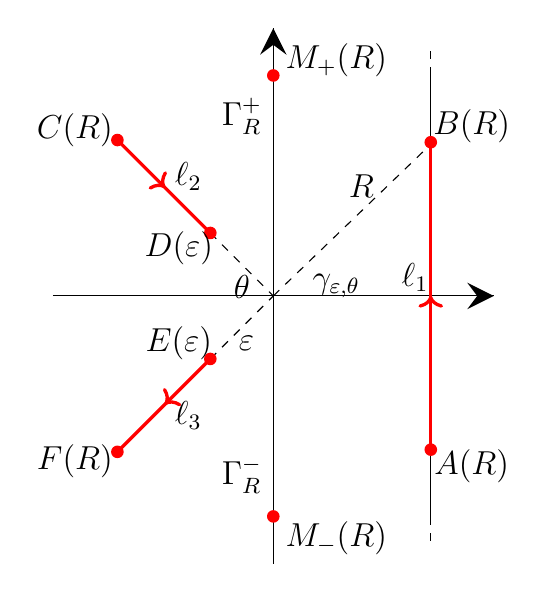
\begin{tikzpicture}[scale=0.4]
		\draw [decoration={markings,mark=at position 1 with
			{\arrow[scale=3,>=stealth]{>}}},postaction={decorate}] (0,-8.5) -- (0,8.5);
		\draw [decoration={markings,mark=at position 1 with
			{\arrow[scale=3,>=stealth]{>}}},postaction={decorate}] (-7,0) -- (7,0);
		\draw[black, dashed] (-2,-2)--(0,0);
		\draw[black, dashed] (-2,2)--(0,0);
		\draw[black] (5,-7) -- (5,-4.88);
		\draw[black] (5,4.88) -- (5,7);
		\draw[black, dashed] (5,-7) -- (5,-8);
		\draw[black, dashed] (5,7) -- (5,8);
		\draw[black, dashed] (0,0)--(4.88,4.70);
		\begin{scope}[very thick,decoration={
				markings,
				mark=at position 0.5 with {\arrow{>}}}
			] 
			\centerarc[red,very thick,postaction={decorate}](0,0)(44:90:7);
			\centerarc[red,very thick,postaction={decorate}](0,0)(90:135:7);
			\draw[red,very thick, postaction={decorate}] (5,-4.88) -- (5,4.88);
			\draw[red,very thick,postaction={decorate}] (-4.88,4.88) -- (-2,2);
			\centerarc[red,very thick,postaction={decorate}](0,0)(135:-135:2.828);
			\draw[red,very thick,postaction={decorate}] (-2,-2)--(-4.88,-4.88);
			\centerarc[red,very thick,postaction={decorate}](0,0)(-135:-90:7);
			\centerarc[red,very thick,postaction={decorate}](0,0)(-90:-44:7);
		\end{scope}
		\fill[red] (5,4.88) circle (0.2);
		\fill[red] (-4.95,4.95) circle (0.2);
		\fill[red] (-2,2) circle (0.2);
		\fill[red] (-2,-2) circle (0.2);
		\fill[red] (-4.95,-4.95) circle (0.2);
		\fill[red] (5,-4.88) circle (0.2);
		\node at (6.3,5.40) {\large $B(R)$};
		\node at (6.3,-5.40) {\large $A(R)$};
		\node at (-6.3,-5.25) {\large $F(R)$};
		\node at (-6.3,5.25) {\large $C(R)$};
		\node at (-3,1.5) {\large $D(\varepsilon)$};
		\node at (-3,-1.5) {\large $E(\varepsilon)$};
		\node at (-0.85,-1.5) {\large $\varepsilon$};
		\centerarc[dashed](0,0)(135:225:0.5);
		\node at (-1,0.3) {\large $\theta$};
		\node at (2.8,3.5) {\large $R$};
		%		\node at (5.6,0.3) {\large $x_0$};
		%		\node at (4.5,2) {\large $r$};
		\fill[red] (0,7) circle (0.2);
		\fill[red] (0,-7) circle (0.2);
		%		\fill[black] (5,0) circle (0.1);
		\node at (2,7.5) {\large $M_+(R)$};
		\node at (2,-7.7) {\large $M_-(R)$};
		\node at (-1,-5.7) {\large $\Gamma_R^-$};
		\node at (-1,5.7) {\large $\Gamma_R^+$};
		\node at (-2.7,3.8)  {\large $\ell_2$};
		\node at (-2.7,-3.8)  {\large $\ell_3$};
		\node at (2,0.3)  {\large $\gamma_{\varepsilon,\theta}$};
		\node at (4.5,0.6)  {\large $\ell_1$};
	\end{tikzpicture}
	\captionof{figure}{\label{fig1}Sketch of the keyhole-type contour.}
\end{minipage}
\begin{minipage}{0.5\linewidth}
	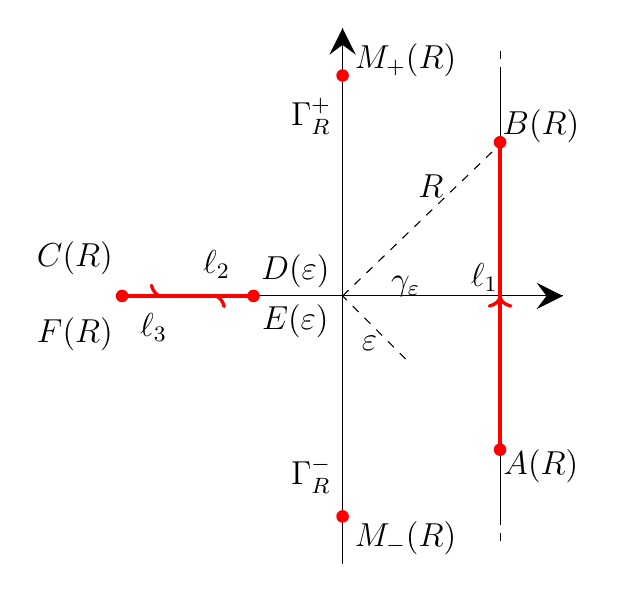
\begin{tikzpicture}[scale=0.4]
		\draw [decoration={markings,mark=at position 1 with
			{\arrow[scale=3,>=stealth]{>}}},postaction={decorate}] (0,-8.5) -- (0,8.5);
		\draw [decoration={markings,mark=at position 1 with
			{\arrow[scale=3,>=stealth]{>}}},postaction={decorate}] (-7,0) -- (7,0);
		\draw[black, dashed] (2,-2)--(0,0);
		%\draw[black, dashed] (-2,2)--(0,0);
		\draw[black] (5,-7) -- (5,-4.88);
		\draw[black] (5,4.88) -- (5,7);
		\draw[black, dashed] (5,-7) -- (5,-8);
		\draw[black, dashed] (5,7) -- (5,8);
		\draw[black, dashed] (0,0)--(4.88,4.70);
		\begin{scope}[very thick,decoration={
				markings,
				mark=at position 0.5 with {\arrow{>}}}
			] 
			\centerarc[red,very thick,postaction={decorate}](0,0)(44:90:7);
			\centerarc[red,very thick,postaction={decorate}](0,0)(90:180:7);
			\centerarc[red,very thick,postaction={decorate}](0,0)(180:90:2.828);
			\centerarc[red,very thick,postaction={decorate}](0,0)(90:0:2.828);
			\centerarc[red,very thick,postaction={decorate}](0,0)(0:-90:2.828);
			\centerarc[red,very thick,postaction={decorate}](0,0)(-90:-180:2.828);
			\draw[red,very thick, postaction={decorate}] (5,-4.88) -- (5,4.88);
			\centerarc[red,very thick,postaction={decorate}](0,0)(-180:-90:7);
			\centerarc[red,very thick,postaction={decorate}](0,0)(-90:-44:7);
		\end{scope}
		\begin{scope}[very thick,decoration={
				markings,
				mark=at position 0.3 with {\arrow{>[left]}}}
			]
			\draw[red,very thick,postaction={decorate}] (-7,0) -- (-2.828,0);
			\draw[red,very thick,postaction={decorate}] (-2.828,0)--(-7,0);
		\end{scope}
		\fill[red] (5,4.88) circle (0.2);
		\fill[red] (-7,0) circle (0.2);
		\fill[red] (-2.828,0) circle (0.2);
		\fill[red] (5,-4.88) circle (0.2);
		\node at (6.3,5.40) {\large $B(R)$};
		\node at (6.3,-5.40) {\large $A(R)$};
		%\node at (-6.3,-5.25) {\large $F(R)$};
		\node at (-8.5,1.2) {\large $C(R)$};
		\node at (-8.5,-1.2) {\large $F(R)$};
		\node at (-1.5,0.8) {\large $D(\varepsilon)$};
		\node at (-1.5,-0.8) {\large $E(\varepsilon)$};
		%\node at (-3,-1.5) {\large $E(\varepsilon)$};
		\node at (0.85,-1.5) {\large $\varepsilon$};
		%\centerarc[dashed](0,0)(135:225:0.5);
		%\node at (-1,0.3) {\large $\theta$};
		\node at (2.8,3.5) {\large $R$};
		%		\node at (5.6,0.3) {\large $x_0$};
		%		\node at (4.5,2) {\large $r$};
		\fill[red] (0,7) circle (0.2);
		\fill[red] (0,-7) circle (0.2);
		%		\fill[black] (5,0) circle (0.1);
		\node at (2,7.5) {\large $M_+(R)$};
		\node at (2,-7.7) {\large $M_-(R)$};
		\node at (-1,-5.7) {\large $\Gamma_R^-$};
		\node at (-1,5.7) {\large $\Gamma_R^+$};
		\node at (-4,1)  {\large $\ell_2$};
		\node at (-6,-1)  {\large $\ell_3$};
		\node at (2,0.3)  {\large $\gamma_{\varepsilon}$};
		\node at (4.5,0.6)  {\large $\ell_1$};
	\end{tikzpicture}
	\captionof{figure}{\label{fig2}Sketch of the keyhole contour.}	
\end{minipage}\\

	Now we deal with various terms separately.
	To deal with the first integral, let $M^+(R)= Ri$ and split the curve $\Gamma_R^+$ into $\Gamma_R^1$ connecting $B(R)$ to $M^+(R)$ and $\Gamma_R^2$ connecting $M^+(R)$ to $C(R)$ so that
	\begin{equation}	\label{29}
		\int_{\Gamma_R^+} F(z; x, t) \, dz  \, = \, \int_{\Gamma_R^1} F(z; x, t) \, dz  + \int_{\Gamma_R^2} F(z; x, t) \, dz.
	\end{equation}
	We begin with $\Gamma_R^1$. Note that, by the Estimation Lemma \cite[Theorem 5.24]{howie}
	\begin{equation}\label{estlemmagen}
		\left| \int_{\Gamma_R^1} F(z x, t) \, dz \right| \, \leq \, \text{length}(\Gamma_R^1) \, \max_{z \in \Gamma_R^1} \left| F(z; x, t) \right|,
	\end{equation}
	where, with an abuse of notation, we denote by $\Gamma_R^1$ also the support of the oriented curve. To evaluate the maximum appearing in \eqref{estlemmagen} we parametrize $\Gamma_R^1$ as follows
	\begin{equation*}
		\Gamma_R^1 \, = \, \ll z \in \mathbb{C}: z = R e^{i\xi}, \xi \in \left[ \xi_{B}(R), \frac{\pi}{2} \right] \rr,
	\end{equation*}
	where $\xi_B(R)= \arctan \lb \frac{r(R)}{a} \rb$.
	Then, for $z = Re^{i\xi} \in \Gamma_R^1$, it holds
	\begin{equation*}
		\left| F(z; x,t) \right| \, =  \frac{\left| \Phi^\dagger(Re^{i\xi}) \right|}{R} e^{Rt\cos \xi -x\Re \Phi (Re^{i\xi})}.
	\end{equation*}
	Without loss of generality we can assume $\xi_B(R)> \frac{\pi}{4}$. First, observe that $\Re \lb Re^{i\xi}\rb= R \cos \xi \geq 0$, for any $\xi \in \left[ \xi_B(R), \frac{\pi}{2} \right]$, and thus, by Item \ref{it:sign} of Lemma \ref{lem:Bern}, we have that $\Re \Phi \lb Re^{i\xi} \rb \geq 0$. Furthermore, it holds that $R \cos \xi \leq R \cos \xi_{B}(R) = a$, for any $\xi \in \left[ \xi_B(R), \frac{\pi}{2} \right]$. Hence, we get
	\begin{equation*}
		\max_{z \in \Gamma_R^1} \left| F(z; x,t) \right| \, \leq \, e^{ta} \max_{\xi \in \left[ \frac{\pi}{4}, \frac{\pi}{2} \right]} \left| \frac{\Phi^{\dagger} \lb Re^{i\xi} \rb}{Re^{i\xi}} \right|
	\end{equation*}
	and thus by Item \ref{it:asymp} of Lemma \ref{lem:Bern} it holds
	\begin{equation}\label{maxtozerogen}
		\lim_{R \to + \infty} \max_{z \in \Gamma_R^1} \left| F(z; x,t) \right| = 0.
	\end{equation}
%	Note now that
%	\begin{equation*}
%		\begin{split}
%			\text{length}(\Gamma_R^1) \, = \,& R \l \frac{\pi}{2} - \xi_B(R) \r = R \l \frac{\pi}{2}-\arctan \frac{r(R)}{a} \r 
%			= \,  \frac{R a}{r(R)} \frac{r(R)}{a} \l \frac{\pi}{2}-\arctan \frac{r(R)}{a} \r.
%		\end{split}	
%	\end{equation*}
%	Since $r(R)= \sqrt{R^2-a^2}$ we obtain
Furthermore, it is not difficult to check that
	\begin{equation}\label{lengthtox0gen}
		\lim_{R \to +\infty}\text{length}(\Gamma_R^1) \, = \, a.
	\end{equation}
	By combining \eqref{maxtozerogen} and \eqref{lengthtox0gen} with \eqref{estlemmagen} we have that
	\begin{equation}\label{firsttozerogen11}
		\lim_{R \to +\infty} \int_{\Gamma_R^1} F(z; x,t) \, dz \, = \, 0.
	\end{equation}	
	Now we deal with the second term in \eqref{29}, i.e. the one on $\Gamma_R^2$.
	%\begin{equation*}
	%	\int_{\Gamma_R^2}F(z; x,t) \, dz \, = \, \int_{\Gamma_R^2} e^{z t} \frac{\Phi^\dagger(z)}{z} e^{-x\Phi(z)} dz.
	%\end{equation*}
	Recalling that $(x,t) \in \mathbb{D}$, let $\delta=t-\mathfrak{b}x>0$ and choose $p > 1$ such that $\frac{t}{p}-\mathfrak{b}x>\frac{\delta}{2}$, that exists since $\lim_{p \to 1}\frac{t}{p}-\mathfrak{b}x=\delta$. Let also $p^\prime >1$ be the conjugate exponent of $p>1$, i.e. $\frac{1}{p}+\frac{1}{p^\prime}=1$. Then we have
%	Let $z = i\zeta$ and set $\widetilde{\Gamma}_R^2:= \ll z \in \mathbb{C}: z=Re^{i\zeta}, \zeta \in \left[ 0, \frac{\pi-\theta}{2} \right] \rr$ to get
%	\begin{equation*}
%		\int_{\Gamma_R^2}F(z; x,t) \, dz \, = \,i \int_{\widetilde{\Gamma}_R^2} e^{i\zeta t} \frac{\Phi^\dagger(i\zeta)}{i\zeta} e^{-x \Phi(i\zeta)} \, d\zeta.
%	\end{equation*} 
%	Let $\delta=t-\mathfrak{b}x>0$ and choose $p > 1$ such that $\frac{t}{p}-\mathfrak{b}x>\frac{\delta}{2}$. This is always possible since we are on $\mathbb{D}$ and since $\frac{t}{p}-\mathfrak{b}x < \delta$ with $\frac{t}{p}-\mathfrak{b}x \to \delta$ as $p\to 1$. Let $q_* \ge 1$ such that $\frac{1}{p}+\frac{1}{q_*}=1$ and $G(\zeta;x,t):= e^{\lambda t/p}(i\zeta)^{-1}\Phi(i\zeta) e^{-x\Phi(i\zeta)}$. We get
	\begin{equation}	\label{220}
	\begin{split}
		\left| \int_{\Gamma_R^2}F(z; x,t) \, dz \right| \,  \leq \, & R \lb \max_{z \in \Gamma_R^2}  \left| \frac{\Phi^\dagger(z)}{z} e^{ \frac{t}{p}z-x\Phi(z)} \right| \rb \lb \int_0^{\frac{\pi-\theta}{2}} e^{-(Rt\sin \xi)/p^\prime} d\xi \rb  \\
		\leq \, & \frac{p^\prime \pi}{t} \lb \max_{z \in \Gamma_R^2}  \left| \frac{\Phi^\dagger(z)}{z} e^{ \frac{t}{p}z-x\Phi(z)} \right| \rb = \, \frac{p^\prime \pi e^{-xq}}{t} \lb \max_{z \in \Gamma_R^2}  \left| \frac{\Phi^\dagger(z)}{z} e^{ \left(\frac{t}{p}-\mathfrak{b}x\right)z-x\Phi^\dagger(z)} \right| \rb, 
	\end{split}	
\end{equation}
%	\begin{equation}	\label{220}
%	\begin{split}
%		\left| \int_{\Gamma_R^2}F(z; x,t) \, dz \right| \, = \, &\left| \int_{\widetilde{\Gamma}_R^2} e^{i\zeta t} \frac{\Phi^\dagger(i\zeta)}{i\zeta} e^{-x \Phi(i\zeta)} \, d\zeta \right|  \\
%		= \, & \left| \int_0^{(\pi-\theta)/2}  e^{iRe^{i\xi}t/q_*} G(Re^{i\xi};x,t) Re^{i\xi} d\xi \right|  \\
%		\leq \, & R \int_0^{(\pi-\theta)/2}  e^{-(Rt \sin \xi )/q_*} \left| G\l Re^{i\xi};x,t \r \right| d\xi  \\
%		\leq \, & R \l \max_{\xi \in \left[ 0, \frac{\pi-\theta}{2} \right]}  \left| G\l Re^{i\xi};x,t \r \right| \r \l \int_0^\pi e^{-(Rt\sin \xi)/q_*} d\xi \r  \\
%		\leq \, & \frac{q_*\pi}{t} \l \max_{z \in \Gamma_R^2}  \left| \frac{\Phi^\dagger(z)}{z} e^{ \frac{t}{p}z-x\Phi(z)} \right| \r \\
%		= \, & \frac{q_*\pi e^{-xq}}{t} \l \max_{z \in \Gamma_R^2}  \left| \frac{\Phi^\dagger(z)}{z} e^{ \left(\frac{t}{p}-\mathfrak{b}x\right)z-x\Phi^\dagger(z)} \right| \r, 
%	\end{split}	
%	\end{equation}
	where in the second inequality we have used Jordan's inequality \cite[eq (2), page 262]{brownchurchill}. Now, consider $g(z)=e^{ \left(\frac{t}{p}-\mathfrak{b}x\right)z-x\Phi^\dagger(z)}$ and observe that, by hypothesis, $g$ is holomorphic on $\C\left(\frac{\pi}{2},\pi-\frac{\theta}{2}\right)$ and continuous on $\overline{\C\left(\frac{\pi}{2},\pi-\frac{\theta}{2}\right)}$. Furthermore, for $z=iR$ we have
	\begin{equation*}
		|g(iR)|=e^{-x\Re \Phi^\dagger(iR)} \le 1,
	\end{equation*}
	since $\Re \Phi^\dagger(iR) \ge 0$ by Item \ref{it:sign} of Lemma \ref{lem:Bern}. For $z=Re^{i\left(\pi-\frac{\theta}{2}\right)}$ we have instead
	\begin{equation*}
		\left|g\left(Re^{i\left(\pi-\frac{\theta}{2}\right)}\right)\right|=e^{-R\left(\frac{t}{p}-\mathfrak{b}x\right)\cos\left(\frac{\theta}{2}\right)-x\Re \Phi^\dagger\left(Re^{i\left(\pi-\frac{\theta}{2}\right)}\right)}.
	\end{equation*}
	Now let us show that for $R$ big enough, $\left|g\left(Re^{i\left(\pi-\frac{\theta}{2}\right)}\right)\right| \le 1$. Indeed,
	\begin{align*}
		\left|g\left(Re^{i\left(\pi-\frac{\theta}{2}\right)}\right)\right|&=\exp\left(-R\cos\left(\frac{\theta}{2}\right)\left(\frac{t}{p}-\mathfrak{b}x+\frac{x}{\cos\left(\frac{\theta}{2}\right)}\frac{\Re \Phi^\dagger\left(Re^{i\left(\pi-\frac{\theta}{2}\right)}\right)}{R}\right)\right).
	\end{align*}
	Once we observe that 
	\begin{equation*}
		\left|\frac{\Re \Phi^\dagger\left(Re^{i\left(\pi-\frac{\theta}{2}\right)}\right)}{R}\right| \le \frac{\left| \Phi^\dagger\left(Re^{i\left(\pi-\frac{\theta}{2}\right)}\right)\right|}{R}
	\end{equation*}
	and we use \eqref{eq:uniformlimcond} to state that $\lim_{R \to +\infty}\frac{\left| \Phi^\dagger\left(Re^{i\left(\pi-\frac{\theta}{2}\right)}\right)\right|}{R}=0$, we know that there exists a constant $C(t,x,p)$ such that for $R>C(t,x,p)$
	\begin{equation*}
		\frac{t}{p}-\mathfrak{b}x+\frac{x}{\cos\left(\frac{\theta}{2}\right)}\frac{\Re \Phi^\dagger\left(Re^{i\left(\pi-\frac{\theta}{2}\right)}\right)}{R} \ge \frac{\delta}{4}.
	\end{equation*}
	Hence, for $R>C(t,x,p)$,
	\begin{align*}
		\left|g\left(Re^{i\left(\pi-\frac{\theta}{2}\right)}\right)\right|&\le \exp\left(-\frac{\delta R\cos\left(\frac{\theta}{2}\right)}{4}\right) \le 1.
	\end{align*}
	On the other hand, $R \in [0,+\infty) \mapsto \left|g\left(Re^{i\left(\pi-\frac{\theta}{2}\right)}\right)\right| \in \R$ is continuous and then the latter inequality implies that there exists $M=M(x,t,p)$ such that $|g(z)| \le M$ for any $z \in \partial \C\left(\frac{\pi}{2},\pi-\frac{\theta}{2}\right)$.
	Furthermore, observe that, for $z=Re^{i\xi}$ with $\xi \in \left(\frac{\pi}{2},\pi-\frac{\theta}{2}\right)$ we have, by \eqref{eq:uniformlimcond}, $|\Re\Phi(z)|\le |\Phi(z)| \le C|z|$, for $|z| \ge 1$. Hence, for $|z| \ge 1$
	\begin{equation*}
		|g(z)|=e^{\frac{t}{p} \Re z+q-x\Re(\Phi(z))} \le e^{q+x|\Re(\Phi(z))|} \le e^{q+xC|z|}.
	\end{equation*}
	The continuity of the function $z \in \overline{\C\left(\frac{\pi}{2},\pi-\frac{\theta}{2}\right)} \mapsto |g(z)|e^{xC|z|} \in \R$ guarantees that there exists a constant $M_1=M_1(x,t,p)>0$ such that 
	\begin{equation*}
		|g(z)| \le M_2e^{xC|z|}, \ \forall z \in \overline{\C\left(\frac{\pi}{2},\pi-\frac{\theta}{2}\right)}.
	\end{equation*}
Since $\pi-\frac{\theta}{2}-\frac{\pi}{2}<\frac{\pi}{2}$, we can use Phragmen-Lindel\"of Theorem (see \cite[Chapter $4$, Exercise $9$, Item (b)]{stein10}) to obtain $|g(z)| \le M$ for any $z \in \overline{\C\left(\frac{\pi}{2},\pi-\frac{\theta}{2}\right)}$.

		
		
%	\begin{equation*}
%		M(x,t,p)=\max\left\{\max_{R \in [0,C(t,x,p)]}\left|g\left(Re^{i\left(\pi-\frac{\theta}{2}\right)}\right)\right|, 1\right\}
%	\end{equation*}
%	so that, for any $z \in \partial \C\left(\frac{\pi}{2},\pi-\frac{\theta}{2}\right)$ it holds $|g(z)| \le M(x,t,p)$. 
%	
%	
%	Thus, define $g_M=\frac{g}{M(x,t,p)}$ so that $g_M$ is holomorphic on $\C\left(\frac{\pi}{2},\pi-\frac{\theta}{2}\right)$, continuous on $\overline{\C\left(\frac{\pi}{2},\pi-\frac{\theta}{2}\right)}$ and $|g_M(z)| \le 1$, for any $z \in \partial \C\left(\frac{\pi}{2},\pi-\frac{\theta}{2}\right)$. Next, observe that, for $z=Re^{i\xi}$ with $\xi \in \left(\frac{\pi}{2},\pi-\frac{\theta}{2}\right)$ we have, by \eqref{eq:uniformlimcond}, $|\Re\Phi(z)|\le |\Phi(z)| \le C|z|$, for $|z| \ge 1$. Hence, for $|z| \ge 1$,
%	\begin{equation*}
%		|g_M(z)|=\frac{|g(z)|}{M(x,t,p)}=\frac{e^{\frac{t}{p}\Re z-x\Re(\Phi(z))}}{M(x,t,p)} \le  \frac{e^{x|\Re\Phi(z)|}}{M(x,t,p)}\le \frac{e^{Cx|z|}}{M(x,t,p)}.
%	\end{equation*}
%Furthermore, define
%\begin{equation*}
%M_1 (x,t,p) = \max_{\substack{z \in \overline{\C\left(\frac{\pi}{2},\pi-\frac{\theta}{2}\right)} \\ |z| \leq 1 }} |g_M(z)| e^{-Cx|z|}
%\end{equation*}	
%and
%\begin{equation*}
%M_2(x,t,p) = \max \l M_1(x,t,p), \frac{1}{M(x,t,p)} \r
%\end{equation*}
%so that $|g_M(z)| \leq M_2(x,t,p) e^{Cx|z|}$, for any $z \in \overline{\C\left(\frac{\pi}{2},\pi-\frac{\theta}{2}\right)}$.
%Finally, observe that
%	\begin{equation*}
%		\pi-\frac{\theta}{2}-\frac{\pi}{2}=\frac{\pi-\theta}{2}=:\frac{\pi}{\beta},
%	\end{equation*}
%	for some $\beta>2$. Hence we can use Phragmen-Lindel\"of Theorem (see \cite[Chapter $4$, Exercise $9$, Item (b)]{stein10}) to obtain $|g_M(z)| \le 1$ for any $z \in \overline{C\left(\frac{\pi}{2},\pi-\frac{\theta}{2}\right)}$, and then $|g(z)| \le M(x,t,p)$.
%	
 Thus, from \eqref{220}, we have
	\begin{equation*}
	\left| \int_{\Gamma_R^2}F(z; x,t) \, dz \right| \le \frac{M(x,t,p)q\pi e^{-xq}}{t} \lb \max_{z \in \Gamma_R^2}  \left| \frac{\Phi^\dagger(z)}{z} \right| \rb.
	\end{equation*}
	Taking the limit as $R \to +\infty$ we finally have
	\begin{equation}\label{230}
		\lim_{R \to +\infty} \int_{\Gamma_R^2} F(z;x,t)\, dz \, = \, 0,
	\end{equation}
	that, combined with \eqref{firsttozerogen11}, leads to
	\begin{equation}	\label{circsopra}
		\lim_{R\to +\infty} \int_{\Gamma_R^+} F(z;x,t) \, dz \, = \,0.
	\end{equation}
	In the same spirit it is possible to see that
	\begin{equation}\label{circsotto}
		\lim_{R \to +\infty} \int_{\Gamma_R^-}F(z;x,t) \, dz \, = \, 0.	
	\end{equation}
	We consider now the integral on $\ell_2$. We have that
	\begin{equation}\label{239}
		\int_{\ell_2} F (z;x,t) dz \,= \, -\int_{\varepsilon}^R \frac{\Phi^\dagger\lb\rho e^{i\lb \pi-\frac{\theta}{2} \rb}\rb}{\rho } e^{-x \Phi \lb \rho e^{i\lb \pi-\frac{\theta}{2} \rb} \rb+t  \rho e^{i \lb \pi-\frac{\theta}{2} \rb}} \, d\rho.
	\end{equation}
	Choose $p,p^\prime > 1$ as above so that, recalling that $\frac{\left|\Phi^\dagger\left(\rho e^{i\left(\pi-\frac{\theta}{2}\right)}\right)\right|}{\rho} \le C$ for $\rho \ge \varepsilon$ by \eqref{eq:uniformlimcond}, we have
	\begin{align}
				&\int_\varepsilon^\infty \left|  \frac{\Phi^\dagger\lb\rho e^{i\lb \pi-\frac{\theta}{2} \rb}\rb}{\rho } e^{-x \Phi \lb \rho e^{i\lb \pi-\frac{\theta}{2} \rb} \rb+t  \rho e^{i \lb \pi-\frac{\theta}{2} \rb}} \right| d\rho \notag \\	= \, & e^{-qx}\int_\varepsilon^\infty \frac{|\Phi^\dagger\lb \rho e^{i \lb \pi-\frac{\theta}{2} \rb} \rb|}{\rho}  \exp \ll {-\rho \cos\left(\frac{\theta}{2}\right) \lb \frac{t}{p}-\mathfrak{b}x +x \frac{\Re \Phi^\dagger \lb \rho e^{i \lb \pi-\frac{\theta}{2} \rb}  \rb}{\rho \cos\left(\frac{\theta}{2}\right)}  \rb } \rr e^{-\rho  \frac{t}{p^\prime} \cos \frac{\theta}{2} }d\rho \notag \\
			\le & CM\int_\varepsilon^\infty e^{-\frac{\rho t}{p^\prime}\cos\left(\frac{\theta}{2}\right)}d\rho <+\infty. \label{richiamatadopo}
	\end{align}
	Hence we can take the limit in \eqref{239} to get
	\begin{equation}	\label{243}
		\lim_{R \to +\infty}\int_{\ell_2} F(z; x,t) \, dz \, = \, -\int_\varepsilon^{+\infty}\frac{\Phi^\dagger\lb\rho e^{i\lb \pi-\frac{\theta}{2} \rb}\rb}{\rho } e^{-x \Phi \lb \rho e^{i\lb \pi-\frac{\theta}{2} \rb} \rb+t  \rho e^{i \lb \pi-\frac{\theta}{2} \rb}} \, d\rho \notag \\ =: \, -I_1(\varepsilon).
	\end{equation}
	Analogously, on $\ell_3$, we have that
	\begin{equation}\label{244}
		\lim_{R \to +\infty}\int_{\ell_3} F(z; x,t) \, dz \, = \, \int_\varepsilon^{+\infty}\frac{\Phi^\dagger\lb\rho e^{i\lb \pi+\frac{\theta}{2} \rb}\rb}{\rho } e^{-x \Phi \lb \rho e^{i\lb \pi+\frac{\theta}{2} \rb} \rb+t  \rho e^{i \lb \pi+\frac{\theta}{2} \rb}} \, d\rho\, =: \, I_2(\varepsilon).
	\end{equation}
	Furthermore, by using the fact that $\overline{\Phi(z)} = \Phi(\overline{z})$ by Schwartz reflection principle (see \cite[Theorem $5.6$]{stein10}), we know that $I_2(\varepsilon) = \overline{I_1(\varepsilon)}$. Hence, taking the limit as $R \to +\infty$ in \eqref{decomp} and using \eqref{circsopra}, \eqref{circsotto}, \eqref{243} and \eqref{244}, we get
	\begin{equation*}
		\begin{split}
				\lim_{b \to +\infty}\int_{a-ib}^{a+ib} e^{z t } 	\,  \frac{\Phi^{\dagger}(z)}{z} e^{-x\Phi(z)} \, dz \, & = \,  I_1(\varepsilon)-\overline{I_1(\varepsilon)} + \, \int_{\gamma_{\varepsilon,\theta}} F(z; x, t) \, dz   =2iI_3(\varepsilon)+\, \int_{\gamma_{\varepsilon,\theta}} F(z; x, t) \, dz,
		\end{split}
	\end{equation*}
	where we denote
	\begin{align}
I_3(\varepsilon):=\int_\varepsilon^{+\infty}\Im\left(\frac{\Phi^\dagger\lb \rho e^{i\left(\pi-\frac{\theta}{2}\right)}\rb}{\rho } e^{-x \Phi \lb \rho e^{i\left(\pi-\frac{\theta}{2}\right)}  \rb+ t \rho e^{i\left(\pi-\frac{\theta}{2}\right)} }\right) \, d\rho.
		\label{beforeepsilon}
	\end{align}
	This proves \eqref{statement1}.
%	Now we would like to take the limit as $\varepsilon \to 0$ to get \eqref{eq:intreptheta}. To do this, let us first handle the integral over $\gamma_{\varepsilon,\theta}$. By the estimation Lemma
%	\begin{equation*}
%		\begin{split}
%			\left| \int_{\gamma_{\varepsilon,\theta}} F(z;x,t) \, dz \right| \, \leq \, & \text{length} (\gamma_{\varepsilon,\theta}) \, \max_{z \in \gamma_{\varepsilon}} \left| F(z; x,t) \right| z
%			= \varepsilon (2\pi - \theta) \max_{z \in \gamma_{\varepsilon}} \left| F(z; x,t) \right|
%		\end{split}
%	\end{equation*}
%	Note now that
%	\begin{equation*}
%		\max_{z \in \gamma_{\varepsilon}} \left| F(z; x,t) \right| \, = \, \frac{1}{\varepsilon}  \max_{z \in \gamma_{\varepsilon}} \left[ \left| \Phi(z) \right| e^{t \Re z -x \Re \Phi (z)} \right]
%	\end{equation*}
%	and thus
%	\begin{align}
%		\left| \int_{\gamma_{\varepsilon,\theta}} F (\lambda; x,t) d\lambda \right| \, \leq \, (2\pi-\theta) \max_{\lambda \in \gamma_{\varepsilon,\theta}} \left[ \left| \Phi^\dagger(\lambda)\right| e^{t\Re \lambda-x\Re \Phi(\lambda)} \right].
%		\label{233}
%	\end{align}
%	By the continuity of $\left| \Phi(z)\right| e^{t\Re z-x\Re \Phi(z)}$ in $\overline{\C\left(\pi-\frac{\theta}{2}\right)}$ (and thus the uniform continuity in $\overline{\C\left(\pi-\frac{\theta}{2}\right)} \cap \{z \in \C: \ |z| \le 1\}$) we clearly have
%	\begin{equation}	\label{cerchietto}
%		\lim_{\varepsilon \to 0} \int_{\gamma_{\varepsilon,\theta}} F(z ;x,t) \, dz\, = \, 0.
%	\end{equation}
%	To take the limit as $\varepsilon \to 0$ in $I_3(\varepsilon)$, just observe that, arguing exactly as in the proof of Proposition \ref{prop:LTthetapi}, we have
%	\begin{align}
%			\int_0^1 \left| \Im  \left(\frac{\Phi^\dagger\l\rho e^{i\l \pi-\frac{\theta}{2} \r}\r}{\rho } e^{-x \Phi \l \rho e^{i\l \pi-\frac{\theta}{2} \r} \r+t  \rho e^{i \l \pi-\frac{\theta}{2} \r}}\right) \right| d\rho \,  \leq \, C  \left(1+\int_0^1  \frac{\left|\Im \Phi\left(\rho e^{i\left(\pi-\frac{\theta}{2}\right)}\right)\right|}{\rho}\right) d\rho<+\infty.
%	\end{align}
%	The statement then follows.
\end{proof}
\begin{rmk}
	Under the hypotheses of Proposition \ref{prop:intreptheta}, if furthermore \begin{equation}\label{eq:intcondtheta}
				\int_0^1\frac{\left|\Im \Phi^\dagger \left(\rho e^{i\left(\pi-\frac{\theta}{2}\right)}\right)\right|}{\rho}d\rho<+\infty
	\end{equation}
	then we can send $\varepsilon \to 0$ in \eqref{statement1}, getting
	\begin{equation*}
		f_\Phi (x,t) \, = \, \frac{1}{\pi} \int_0^{+\infty}\Im\left(\frac{\Phi^\dagger\lb \rho e^{i\left(\pi-\frac{\theta}{2}\right)}\rb}{\rho } e^{-x \Phi \lb \rho e^{i\left(\pi-\frac{\theta}{2}\right)}  \rb+ t \rho e^{i\left(\pi-\frac{\theta}{2}\right)} }\right) \, d\rho.
	\end{equation*}
\end{rmk}
A similar integral representation holds also for $\bar{\mu}_\phi^{\ast n}$. The proof is similar to the one of Proposition \ref{prop:intreptheta}, where we substitute the term $\frac{\phi^\dagger(z)}{z}e^{-x\phi(z)}$ with $\left(\frac{\phi^\dagger(z)}{z}\right)^n$. For such a reason, we only underline the parts of the proof that are actually different.
\begin{prop}
	\label{lem:convtail}
	With the same notation of Proposition \ref{prop:intreptheta}, under \eqref{eq:extensionA3} and \eqref{eq:uniformlimcond}, for $n \ge 0$, it holds that, for any $t>0$,
	\begin{equation}\label{convcode}
		\bar{\mu}_\Phi^{\ast n} (t) = \frac{1}{\pi} \int_{\varepsilon}^{+\infty} \Im \left[ \lb \frac{\Phi^\dagger \lb \rho e^{i \lb \pi-\frac{\theta}{2} \rb} \rb}{\rho e^{i \lb \pi-\frac{\theta}{2} \rb}} \rb^n e^{i \lb \pi-\frac{\theta}{2} \rb}e^{t\rho e^{i \lb \pi-\frac{\theta}{2} \rb}} \right] d\rho +\frac{1}{2\pi i} \int_{\gamma_{\varepsilon,\theta}} e^{tz} \lb \frac{\phi^\dagger (z)}{z} \rb^n dz.
	\end{equation}
%	 Furthermore, it is true that the function $(0, +\infty) \mapsto \bar{\nu}_\phi^{\star n} (t)$, has, for any $n=1,2,\cdots$, derivatives of all order $r \geq 0$, such that
%	\begin{equation}
%		\frac{d^r}{dt^r} \bar{\mu}_\Phi^{n\star} (t) 
%		= \frac{1}{\pi} \int_{\varepsilon}^{+\infty} \Im \left[  \frac{\l\Phi^\dagger \l \rho e^{i \l \pi-\frac{\theta}{2} \r} \r\r^n}{\rho^{n-r}e^{i(n-r-1)\l \pi-\frac{\theta}{2} \r}}  e^{t\rho e^{i \l \pi-\frac{\theta}{2} \r}} \right] d\rho -\frac{1}{2\pi i} \int_{\gamma_{\varepsilon,\theta}} e^{tz}  \frac{\l\phi^\dagger (z)\r^n}{z^{n-r}}  dz.
%		\label{derivatecode}
%	\end{equation}
\end{prop}
\begin{proof}
	Setting $F_n(z;t)=\left(\frac{\phi^\dagger(z)}{z}\right)^ne^{tz}$ the proof follows as the one in Proposition \ref{prop:intreptheta}. The main differences concern integrals over $\Gamma^2_R$ and $\ell_2$. First, by Jordan's inequality \cite[eq. (2), page 262]{brownchurchill},
	\begin{equation*}
		\left|\int_{\Gamma^2_R}F_n(z;t)dz\right| \le \frac{\pi}{t}\left(\max_{z \in \Gamma_R^2}\left|\frac{\Phi^\dagger(z)}{z}\right|^n\right) \to 0, \mbox{as $R\to\infty$},
	\end{equation*}
	where the limit holds by assumption \eqref{eq:uniformlimcond}. Concerning the integral over $\ell_2$, observe that
	\begin{equation*}
		\int_{\varepsilon}^{\infty}|F_n\left(\rho e^{i\left(\pi-\frac{\theta}{2};t\right)};t\right)|dz \le \int_{\varepsilon}^{\infty}e^{-\rho t \cos\left(\frac{\theta}{2}\right)}\left|\frac{\Phi^\dagger\left(\rho e^{i\left(\pi-\frac{\theta}{2}\right)}\right)}{\rho}\right|^nd\rho \le C\int_{\varepsilon}^{\infty}e^{-\rho t \cos\left(\frac{\theta}{2}\right)} d\rho<+\infty,
	\end{equation*}
	where we have used the fact that $\left|\frac{\Phi^\dagger\left(\rho e^{i\left(\pi-\frac{\theta}{2}\right)}\right)}{\rho}\right|^n$ is bounded for $\rho \ge \varepsilon$ by assumption \eqref{eq:uniformlimcond}.
\end{proof}
Now we are ready to prove Theorem \ref{thm:smoothfmu} by using the previously obtained integral representations.
\begin{proof}[Proof of Theorem \ref{thm:smoothfmu}]
	Let us first prove that $\bar{\mu}_\phi^{\ast n} \in C^\infty(0,+\infty)$. To do this, fix $\varepsilon>0$, let $l \ge 1$ and $[t_1,t_2]\subset (0,+\infty)$. Let $F_n(z;t)=\left(\frac{\phi^\dagger(z)}{z}\right)^ne^{tz}$. Then $\frac{\partial^l}{\partial t^l}F_n(z,t)=z^l\left(\frac{\phi^\dagger(z)}{z}\right)^ne^{tz}$ is continuous for $(z,t) \in \gamma_{\varepsilon,\theta} \times [t_1,t_2]$, where, with an abuse of notation, $\gamma_{\varepsilon,\theta}$ is the support of the parametrized curve defined in Proposition \ref{prop:intreptheta}. Then we have
	\begin{equation}\label{eq:upboundovereps}
		\left|\frac{\partial^l}{\partial t^l}F_n(z,t)\right| \le \max_{(z,t) \in \gamma_{\varepsilon,\theta} \times [t_1,t_2]}\left|z^l\left(\frac{\phi^\dagger(z)}{z}\right)^ne^{tz}\right|
	\end{equation}
	where the right-hand side is constant, hence integrable over $\gamma_{\varepsilon,\theta}$. Next, let
	\begin{equation*}
		G_n(\rho,t)=\Im \left[ \lb \frac{\Phi^\dagger \lb \rho e^{i \lb \pi-\frac{\theta}{2} \rb} \rb}{\rho e^{i \lb \pi-\frac{\theta}{2} \rb}} \rb^n e^{i \lb \pi-\frac{\theta}{2} \rb}e^{t\rho e^{i \lb \pi-\frac{\theta}{2} \rb}} \right]
	\end{equation*}
	and observe that
	\begin{equation*}
		\frac{\partial^l}{\partial t^l}G_n(\rho,t)=\Im \left[ \lb \frac{\Phi^\dagger \lb \rho e^{i \lb \pi-\frac{\theta}{2} \rb} \rb}{\rho e^{i \lb \pi-\frac{\theta}{2} \rb}} \rb^n \rho^l e^{i(l+1) \lb \pi-\frac{\theta}{2} \rb}e^{t\rho e^{i \lb \pi-\frac{\theta}{2} \rb}} \right].
	\end{equation*}
	For $\rho \ge \varepsilon$ and $t \in [t_1,t_2]$, we have
	\begin{equation}\label{eq:contrder2}
		\left|\frac{\partial^l}{\partial t^l}G_n(\rho,t)\right| \le C e^{-t_1 \rho \cos \frac{\theta}{2}} \rho^l,
	\end{equation}
	since $\left|\frac{\Phi^\dagger\left(\rho e^{i\left(\pi-\frac{\theta}{2}\right)}\right)}{\rho}\right|^n$ is bounded for $\rho \ge \varepsilon$ by assumption \eqref{eq:uniformlimcond}. Observe that the right-hand side of \eqref{eq:contrder2} is integrable over $(\varepsilon,+\infty)$. Hence, by \eqref{eq:upboundovereps} and \eqref{eq:contrder2} and the fact that $l \ge 1$ is arbitrary, we can differentiate $l$ times inside the integrals in \eqref{convcode}, getting	
	\begin{equation}
		\frac{d^r}{dt^r} \bar{\mu}_\Phi^{\ast n} (t) 
		= \frac{1}{\pi} \int_{\varepsilon}^{+\infty} \Im \left[  \frac{\lb\Phi^\dagger \lb \rho e^{i \lb \pi-\frac{\theta}{2} \rb} \rb\rb^n}{\rho^{n-r}e^{i(n-r-1)\lb \pi-\frac{\theta}{2} \rb}}  e^{t\rho e^{i \lb \pi-\frac{\theta}{2} \rb}} \right] d\rho +\frac{1}{2\pi i} \int_{\gamma_{\varepsilon,\theta}} e^{tz}  \frac{\lb\phi^\dagger (z)\rb^n}{z^{n-r}}  dz.
		\label{derivatecode}
	\end{equation}
	This ends the first part of the proof.
	
	Now let us prove that $f_\Phi \in C^\infty(\mathbb{D})$. To do this, fix any $k,l \ge 0$, $0<t_1<t_2$ and $0<x_1<x_2<t_1/\mathfrak{b}$, recalling that any $(x,t) \in \mathbb{D}$ admits a compact neighbourhood of the form $[x_1,x_2]\times [t_1,t_2]$ specified before. Let $F(z;x,t)=\frac{\phi^\dagger(z)}{z}e^{-x\phi(z)+tz}$ and observe that
	\begin{equation*}
		\frac{\partial^k}{\partial x^k}\frac{\partial^l}{\partial t^l}F(z;x,t)=(-1)^k\frac{z^l\phi^\dagger(z)(\phi(z))^k}{z}e^{-x\phi(z)+tz}.
\end{equation*} 
	The latter is continuous over $\gamma_{\varepsilon,\theta} \times [x_1,x_2]\times [t_1,t_2]$ and then
	\begin{equation}\label{eq:smoothf1}
		\left|\frac{\partial^k}{\partial x^k}\frac{\partial^l}{\partial t^l}F(z;x,t)\right|\le \max_{(z,x,t) \in \gamma_{\varepsilon,\theta} \times [x_1,x_2]\times [t_1,t_2]}\left|\frac{z^l\phi^\dagger(z)(\phi(z))^k}{z}e^{-x\phi(z)+tz}\right|,
	\end{equation}
	where the right-hand side is a constant and then it is integrable over $\gamma_{\varepsilon,\theta}$. Now set
	\begin{equation*}
		G(\rho;x,t)=\Im\left(\frac{\Phi^\dagger\lb \rho e^{i\left(\pi-\frac{\theta}{2}\right)}\rb}{\rho } e^{-x \Phi \lb \rho e^{i\left(\pi-\frac{\theta}{2}\right)}  \rb+ t \rho e^{i\left(\pi-\frac{\theta}{2}\right)} }\right)
\end{equation*}
	and observe that
	\begin{equation*}
		\frac{\partial^k}{\partial x^k}\frac{\partial^l}{\partial t^l}G(\rho;x,t)=(-1)^k\Im\left(\frac{\Phi^\dagger\lb \rho e^{i\left(\pi-\frac{\theta}{2}\right)}\rb\left(\Phi\left(\rho e^{i\left(\pi-\frac{\theta}{2}\right)}\right)\right)^k}{\rho^{k+1}}\rho^{l+k} e^{il\left(\pi-\frac{\theta}{2}\right)}e^{-x \Phi \lb \rho e^{i\left(\pi-\frac{\theta}{2}\right)}  \rb+ t \rho e^{i\left(\pi-\frac{\theta}{2}\right)} }\right).
	\end{equation*}
	Recalling that $\left|\frac{\Phi^\dagger\lb \rho e^{i\left(\pi-\frac{\theta}{2}\right)}\rb\left(\Phi\left(\rho e^{i\left(\pi-\frac{\theta}{2}\right)}\right)\right)^k}{\rho^{k+1}}\right|$ is bounded as $\rho \ge \varepsilon$ and setting $p,p^\prime >1$ and $M>0$ as in the proof of Proposition \ref{prop:intreptheta} with respect to $t_2$ and $x_1$, we have
	\begin{equation}\label{smoothfphi2}
		\left|\frac{\partial^k}{\partial x^k}\frac{\partial^l}{\partial t^l}G(\rho;x,t)\right|\le CM e^{-\frac{\rho t_1}{p^\prime}\cos \frac{\theta}{2}},
	\end{equation}
	 where the right-hand side is integrable on $(\varepsilon,+\infty)$. Hence, since $k,l \ge 0$ are arbitrary, we can differentiate $k$ times in $x$ and $l$ times with respect to $t$ in \eqref{statement1}, to get that $f_\Phi \in C^\infty(\mathbb{D})$ and
	 \begin{align}\label{derivatefphi}
	 	\begin{split}
	 	\frac{\partial^k}{\partial x^k}\frac{\partial^l}{\partial t^l}f_\phi(x,t)&= \frac{(-1)^k}{\pi} \int_\varepsilon^{+\infty}\Im\left(\frac{\Phi^\dagger\lb \rho e^{i\left(\pi-\frac{\theta}{2}\right)}\rb\lb\Phi\lb \rho e^{i\left(\pi-\frac{\theta}{2}\right)}\rb\rb^{k}}{\rho^{1-l} e^{-i l \left(\pi-\frac{\theta}{2}\right)}}e^{-x \Phi \lb \rho e^{i\left(\pi-\frac{\theta}{2}\right)}  \rb+ t \rho e^{i\left(\pi-\frac{\theta}{2}\right)} }\right) \, d\rho \\
	 	&+\frac{(-1)^k}{2\pi i}\int_{\gamma_{\varepsilon,\theta}} \frac{\Phi^\dagger(z)(\Phi(z))^{k}}{z^{1-l}}e^{-x\Phi(z)+tz}dz.
		\end{split} 
	 \end{align}
\end{proof}
A slight modification of the previous arguments lead to the proof of Proposition \ref{prop:extcont}.
\begin{proof}[Proof of Proposition \ref{prop:extcont}]
	Since $\phi$ is a complete Bernstein function that can be extended by continuity over $\overline{\C(0,\pi)}$ with extension $\phi_+$, then, by using the relation $\overline{\phi(z)}=\phi(\overline{z})$, it is clear that it can be also extended by continuity over $\overline{\C(-\pi,0)}$. If we denote such an extension $\phi_-$, for any $z \in \overline{\C(0,\pi)}$ we get
	\begin{equation*}
		\overline{\phi_+(z)}=\phi_-(\overline{z}).
	\end{equation*}
	The proof is then carried on exactly as in Propositions \ref{prop:intreptheta} and \ref{lem:convtail}, by setting $\theta=0$ (see Figure \ref{fig2}), where we use $\phi^\dagger$ when we integrate over $\ell_1$, $\Gamma_R^+$, $\Gamma_R^-$ and $-\gamma_\varepsilon$, $\phi^\dagger_+$ over $\ell_2$ and $\phi^\dagger_-$ over $\ell_1$.
\end{proof}
Let us give, for completeness, the integral representations for $G_\Phi$ and $g_\Phi$, whose proof is identical to the one of Proposition \ref{prop:intreptheta}.
\begin{prop}
	Let $\Phi$ be the Laplace exponent of a potentially killed subordinator satisfying assumptions \ref{eq:extensionA3} and \eqref{eq:uniformlimcond} for some $\theta \in (0,\pi)$. Fix any $\varepsilon>0$ and let $\gamma_{\varepsilon,\theta}$ be defined as in Proposition \ref{prop:intreptheta}. Then, on $\mathbb{D}$,
	\begin{equation}\label{statementG}
		\begin{split}
			G_\Phi (x,t) \, = \,& \frac{1}{\pi} \int_\varepsilon^{+\infty}\Im\left(\frac{e^{-x \Phi \lb \rho e^{i\left(\pi-\frac{\theta}{2}\right)}  \rb+ t \rho e^{i\left(\pi-\frac{\theta}{2}\right)} }}{\rho} \right) \, d\rho  +\frac{1}{2\pi i}\int_{\gamma_{\varepsilon,\theta}} \frac{e^{-x\Phi(z)+tz}}{z}dz.
		\end{split}
	\end{equation}
	In particular, $G_\Phi \in C^\infty(\mathbb{D})$, $g_\Phi \in C^\infty(\mathbb{D})$ is well defined and for any $k,l \ge 0$ we have
	\begin{equation}\label{statementG2}
		\begin{split}
			\frac{\partial^k}{\partial x^k}\frac{\partial^l}{\partial t^l}g_\Phi (x,t) \, = \,& \frac{1}{\pi} \int_\varepsilon^{+\infty}\Im\left(\left(\Phi\left(\rho e^{i\left(\pi-\frac{\theta}{2}\right)}\right)\right)^k\rho^le^{il\left(\pi-\frac{\theta}{2}\right)}e^{-x \Phi \lb \rho e^{i\left(\pi-\frac{\theta}{2}\right)}  \rb+ t \rho e^{i\left(\pi-\frac{\theta}{2}\right)} } \right) \, d\rho  \\
			&+\frac{1}{2\pi i}\int_{\gamma_{\varepsilon,\theta}} (\Phi(z))^kz^le^{-x\Phi(z)+tz}dz.
		\end{split}
	\end{equation}
\end{prop}

%The following statement, which is of independent interest, plays a central role in the proof of Theorem \ref{thm:seriespi}, as it guarantees the smoothness of the $n$-fold convolution appearing in \eqref{coeff}.
%\begin{lem}
%	\label{lem:convtail}
%	Suppose that \eqref{eq:extensionA3} and \eqref{eq:uniformlimcond} are verified. Define, for a fixed $\varepsilon >0$, the set $\gamma_{\varepsilon,\theta} = \ll z \in \mathbb{C}: z=\varepsilon e^{i\xi}, \xi \in \left[ \frac{\theta}{2}-\pi, \pi- \frac{\theta}{2} \right] \rr$. Then we have, for any $n =1,2 \cdots$,  that
%	\begin{equation}\label{convcode}
%		\bar{\mu}_\Phi^{n\star} (t) = \frac{1}{\pi} \int_{\varepsilon}^{+\infty} \Im \left[ \l \frac{\Phi^\dagger \l \rho e^{i \l \pi-\frac{\theta}{2} \r} \r}{\rho e^{i \l \pi-\frac{\theta}{2} \r}} \r^n e^{i \l \pi-\frac{\theta}{2} \r}e^{t\rho e^{i \l \pi-\frac{\theta}{2} \r}} \right] d\rho -\frac{1}{2\pi i} \int_{\gamma_{\varepsilon,\theta}} e^{tz} \l \frac{\phi^\dagger (z)}{z} \r^n dz,
%	\end{equation}
%	for any $t>0$. Furthermore, it is true that the function $(0, +\infty) \mapsto \bar{\nu}_\phi^{\star n} (t)$, has, for any $n=1,2,\cdots$, derivatives of all order $r \geq 0$, such that
%	\begin{equation}
%		\frac{d^r}{dt^r} \bar{\mu}_\Phi^{n\star} (t) 
%		= \frac{1}{\pi} \int_{\varepsilon}^{+\infty} \Im \left[  \frac{\l\Phi^\dagger \l \rho e^{i \l \pi-\frac{\theta}{2} \r} \r\r^n}{\rho^{n-r}e^{i(n-r-1)\l \pi-\frac{\theta}{2} \r}}  e^{t\rho e^{i \l \pi-\frac{\theta}{2} \r}} \right] d\rho -\frac{1}{2\pi i} \int_{\gamma_{\varepsilon,\theta}} e^{tz}  \frac{\l\phi^\dagger (z)\r^n}{z^{n-r}}  dz.
%		\label{derivatecode}
%	\end{equation}
%\end{lem}

	
	\section{Proofs}\label{sec:proofs}
	%\subsection{Proofs for large asymptotic behaviour}
\subsection{Proofs for Subsection \ref{subsec:L}}
\label{subsec:asymp}
In this part we provide proofs for for subsection \ref{subsec:L}. We start with some preliminary results.
\begin{prop}\label{prop:D}
	Let $\Phi$ be the Laplace exponent of a potentially killed subordinator  and  \eqref{def:condiA} holds for some $L>0$. Let $t=t(x)$ be such that $t/x \downarrow \mathfrak{b}$ and $a_*=a_*(x)$ be the unique solution of $\Phi'(a_*)=\frac{t}{x}\in\lbrb{\mathfrak{b},\Phi'(0)}$. Then $\lim_{x \to \infty}a_*=\infty$ and, for $x$ large enough, 
	\begin{equation}\label{eq:ineq}
		\begin{split}
			&a_*>\frac{Me^{-1}}{\frac{t}{x}-\mathfrak{b}}.
		\end{split}
	\end{equation}
\end{prop}
\begin{proof}
	First of all, observe that, since $t/x \downarrow \mathfrak{b}$ and $\Phi'$ is decreasing with $\lim_{z \to \infty}\Phi'(z)=\mathfrak{b}$, we have $\lim_{x \to \infty}a_*=\infty$. Furthermore, for any $M<L$, using the second inequality of \eqref{eq:P}, we get
	\[Me^{-1}<\limi{x}\frac{a_*\lbrb{\Phi'(a_*)-\mathfrak{b}}}{\ln(a_*)}=\limi{x}\frac{a_*\lbrb{\frac{t}{x}-\mathfrak{b}}}{\ln(a_*)}.\]
	This shows that for all $x$ and therefore $a_*$ large enough
	\[\frac{a_*}{\ln(a_*)}>\frac{Me^{-1}}{\frac{t}{x}-\mathfrak{b}}.\]
	This concludes the proof.
\end{proof}
Now we are ready to prove the main theorem concerning the asymptotic behaviour.
\begin{proof}[Proof of Theorem \ref{thm:mainL}]
Fix $k,l\geq 0$ and assume that $x>x_{0}(k+l,L)$, see Theorem \ref{thm:regularityfphi1}. Then, for any $a>0$, by \eqref{intreprder1} it holds
	\begin{equation}\label{def:derf}
		\frac{\partial^k\partial ^l }{\partial x^k\partial t^l}\fP{x,t}=\frac{(-1)^k}{2\pi}\int_{-\infty}^\infty \frac{\Phi^{\dagger}(\ab)\Phi^{k}(\ab)}{\lbrb{\ab}^{1-l}}e^{-x\Phi(\ab)+t\lbrb{\ab}}db=:I(x,t).
	\end{equation}
	%where we have simply differentiated the inversion of the Laplace transform in \eqref{eq:LT1} which is possible thanks to the absolute integrability of the expression in \eqref{intreprder1}.
	Let $t=t(x)$ be as in the statement of the theorem and $a_*:=a(x)$ be the solution to the equation
	\begin{equation*}
		\Phi'(a_*)=\frac{t}{x}\in\lbrb{\mathfrak{b},\Phi'(0^+)},
	\end{equation*}
	which exists and is unique thanks to the fact $\Phi'(x)$ is decreasing with $\limi{x}\Phi'(x)=\mathfrak{b}$, see Item \eqref{it:phi'} of Lemma \ref{lem:Bern}.
	Choosing this $a_*$ for the line of inversion we get
	\begin{equation}\label{eq:f1}
		I(x,t)=\frac{(-1)^k}{2\pi}e^{a_*t-x\Phi(a_*)}\IntII\frac{\Phi^{\dagger}(a_*+ib)\Phi^{k}(a_*+ib)}{\lbrb{a_*+ib}^{1-l}}e^{ibt -x\lbrb{\Phi(a_*+ib)-\Phi(a_*)}}db,
	\end{equation}
	where the choice of $a_*$ minimizes the function  $a \in (0,+\infty)\mapsto (at-x\Phi(a)) \in \R$. Recalling that $t(x)/x\downarrow\mathfrak{b}$, we get that $\limi{x}a_*\to\infty$ by Proposition \ref{prop:D}. From now on, each time we write $\so{\cdot}$ or $\bo{\cdot}$, we imply that $x \to \infty$.
	We  split the region of integration. For any $\varepsilon>0$, which  will subsequently be chosen to depend on $a_*$, we set  $\Ic_{\varepsilon}:=[-a_*\varepsilon,a_*\varepsilon], \Jc_\varepsilon:=\Ic^c_\varepsilon$. Put 
		\begin{equation}\label{def:Ie}
		I_\varepsilon(x,t):=\frac{(-1)^k}{2\pi}e^{a_*t-x\Phi(a_*)}\int_{\Ic_{\varepsilon}}\frac{\Phi^{\dagger}(a_*+ib)\Phi^{k}(a_*+ib)}{\lbrb{a_*+ib}^{1-l}}e^{ibt -x\lbrb{\Phi(a_*+ib)-\Phi(a_*)}}db
	\end{equation}
and
\begin{equation}\label{def:Je1}
	\begin{split}
		J(a_*,b)&:=\frac{\Phi^{\dagger}(a_*+ib)\Phi^{k}(a_*+ib)}{\lbrb{a_*+ib}^{1-l}}.
	\end{split}
\end{equation}
	Using Taylor's formula we get
\begin{equation}\label{def:Tay}
	\begin{split}
		&\Phi(a_*+ib)-\Phi(a_*)=ib\frac{t}{x}-\frac{b^2}{2}\Phi''(a_*)-i\frac{b^3}{3!}\Phi'''(a_*+ib\theta(a_*,b)),
	\end{split}
\end{equation}
where we have used the definition of $a_*$ in \eqref{eq:a*} and note that $0\leq\theta(a_*,b)\leq 1$. Hence, with
\begin{equation*}
	\begin{split}
		U(a_*,b):=&ibt -x\lbrb{\Phi(a_*+ib)-\Phi(a_*)}-x\frac{b^2}{2}\Phi''(a_*)=-ix\frac{b^3}{3!}\Phi'''(a_*+ib\theta(a_*,b)),
	\end{split}
\end{equation*}
we have  for the integral in \eqref{def:Ie}
\begin{equation}\label{def:I'}
	\begin{split}
		&\int_{\Ic_{\varepsilon}}J(a_*,b)e^{ibt -x\lbrb{\Phi(a_*+ib)-\Phi(a_*)}}db=\int_{\Ic_{\varepsilon}}J(a_*,b)e^{\frac{b^2}{2}x\Phi''(a_*)\lbrb{1+2\frac{U(a_*,b)}{xb^2\Phi''(a_*)}}}db\\&=\!\frac{1}{\sqrt{-\Phi''(a_*)x}}\int_{-\varepsilon a_*\sqrt{-\Phi''(a_*)x}}^{\varepsilon a_*\sqrt{-\Phi''(a_*)x}}J\lbrb{a_*,\frac{u}{\sqrt{-\Phi''(a_*)x}}}\!e^{-\frac{u^2}{2}\lbrb{1-2\frac{U\lbrb{a_*,u/\sqrt{-\Phi''(a_*)x}}}{u^2}}}\!\!du,
	\end{split}	
\end{equation}
where we have used that $\Phi''(y)<0$, for $y>0$, see Item \eqref{it:phi'} of Lemma \ref{lem:Bern}. 	Here, we need \eqref{def:condiB}, that is $\limsupi{y}y\Phi'''(y)/(-\Phi''(y))=K<\infty$.  Indeed, due to this and since $\abs{\Phi'''(z)}\leq \Phi'''(\Re(z))$, for $\Re(z)>0$, see Item \ref{it:real} in Lemma \ref{lem:Bern}, we have thanks to the definition of $U(a_*,b)$ that for all $x$ and henceforth for all $a_*$ large enough the inequality 
\begin{equation*}
	\begin{split}
		&\sup_{ |u|\leq \varepsilon a_*\sqrt{-\Phi''(a_*)x}}\frac{2}{u^2}\abs{U\lbrb{a_*,\frac{u}{\sqrt{-\Phi''(a_*)x}}}}\leq  \sup_{ |u|\leq\varepsilon a_*\sqrt{-\Phi''(a_*)x}}\frac{x|u|}{3x^{\frac32}\lbrb{-\Phi''(a_*)}^{\frac32}}\Phi'''(a_*)\leq  \frac{2K}{3}\varepsilon
	\end{split}
\end{equation*}
holds true.	Next, we choose
\begin{equation}\label{eq:varesp}
	\begin{split}
		&\varepsilon(a_*):=\varepsilon(a_*,x)=\frac{g(a_*,x)}{ a_*\sqrt{-\Phi''(a_*)x}}
	\end{split}
\end{equation}
for some $g(y,x)$ going as slowly to infinity, as $x,y\to\infty$, as we wish. Then, we get
\begin{equation*}
	\begin{split}
		\sup_{ |u|\leq g(a_*)}\frac{2}{u^2}\abs{U\lbrb{a_*,\frac{u}{\sqrt{-\Phi''(a_*)x}}}}\leq  \frac{2K}{3}\frac{g(a_*) }{a_*\sqrt{-\Phi''(a_*)x}}.
	\end{split}
\end{equation*}
	Since from Proposition \ref{prop:D0} $\limi{y}-y^2\Phi''(y)=\infty$ then, for any $g(a_*,x)=\so{a_*\sqrt{-\Phi''(a_*)x}}$, we have
\begin{equation}\label{eq:estU}
	\begin{split}
		\sup_{ |u|\leq g(a_*,x)}\frac{2}{u^2}\abs{U\lbrb{a_*,\frac{u}{\sqrt{-\Phi''(a_*)x}}}}=\bo{\frac{g(a_*,x) }{a_*\sqrt{-\Phi''(a_*)x}}}.
	\end{split}
\end{equation}
Next, setting 
\begin{equation}\label{def:tJ}
	\begin{split}
		&\tilde{J}(a_*,u)=J(a_*,u)-J(a_*,0),
	\end{split}
\end{equation}
we get that from \eqref{def:I'}
\begin{equation}\label{def:I'1}
	\begin{split}
	&\int_{\Ic_{\varepsilon}}J(a_*,b)e^{ibt -x\lbrb{\Phi(a_*+ib)-\Phi(a_*)}}db	=\frac{J(a_*,0)}{\sqrt{-\Phi''(a_*)x}}\int_{-g(a_*,x)}^{g(a_*,x)}e^{-\frac{u^2}{2}\lbrb{1+\bo{\frac{g(a_*,x) }{a_*\sqrt{-\Phi''(a_*)x}}}}}du\\
		&+\frac{1}{\sqrt{-\Phi''(a_*)x}}\int_{-g(a_*,x)}^{g(a_*,x)}\tilde{J}\lbrb{a_*,\frac{u}{\sqrt{-\Phi''(a_*)x}}}e^{-\frac{u^2}{2}\lbrb{1+\bo{\frac{g(a_*,x) }{a_*\sqrt{-\Phi''(a_*)x}}}}}du\\
		&=:H_1(a_*,x)+H_2(a_*,x).
	\end{split}
\end{equation}
Clearly,
\begin{equation*}
	\begin{split}
		H_1(a_*,x)&=\frac{1}{\sqrt{-\Phi''(a_*)}x}\frac{\Phi^\dagger(a_*)\Phi^{k}(a_*)}{a^{1-l}_*}\int_{-g(a_*,x)}^{g(a_*,x)}e^{-\frac{u^2}{2}\lbrb{1+\bo{\frac{g(a_*,x) }{a_*\sqrt{-\Phi''(a_*)x}}}}}du\\
		&=\frac{\lbrb{1+\bo{\frac{g(a_*,x) }{a_*\sqrt{-\Phi''(a_*)x}}}}}{\sqrt{-\Phi''(a_*)x}}\frac{\Phi^\dagger(a_*)\Phi^{k}(a_*)}{a^{1-l}_*}\int_{-g(a_*,x)}^{g(a_*,x)}e^{-\frac{u^2}{2}}du.
	\end{split}
\end{equation*}
	Since $\limi{y,x}g(y,x)=\infty$ we  get further that 
\begin{equation}\label{eq:H1}
	\begin{split}
		&	H_1(a_*,x)=\frac{\sqrt{2\pi}}{\sqrt{-\Phi''(a_*)x}}\frac{\Phi^\dagger(a_*)\Phi^{k}(a_*)}{a^{1-l}_*}\lbrb{1+\bo{\frac{g(a_*,x) }{a_*\sqrt{-\Phi''(a_*)x}}}+\bo{\frac{e^{-\frac{g^2(a_*,x)}{2}}}{g(a_*,x)}}},
	\end{split}
\end{equation}
	where we have used the well-known
\[\int_{u>y}e^{-\frac{u^2}{2}}du\simi C \frac{1}{y}e^{-\frac{y^2}{2}}.\]
 From the definition of $J$, see \eqref{def:Je1}, used in \eqref{def:tJ} we easily get that
\begin{equation}\label{def:tJ1}
	\begin{split}
	\tilde{J}\lbrb{a_*,b}	&=\frac{\Phi^{\dagger}(a_*+ib)\Phi^{k}(a_*+ib)-\Phi^{\dagger}(a_*)\Phi^{k}(a_*)}{\lbrb{a_*+ib}^{1-l}}+\Phi^{\dagger}(a_*)\Phi^{k}(a_*)\lbrb{\frac{1}{\lbrb{a_*+ib}^{1-l}}-\frac{1}{a^{1-l}_*}}\\
	&=	\tilde{J}_1\lbrb{a_*,b}+\tilde{J}_2\lbrb{a_*,b}.
	\end{split}
\end{equation}
We shall use this to estimate for $|u|\leq g(a_*,x)$ the right-hand side of the inequality
\begin{equation}\label{aim}
	\begin{split}
		&\abs{\tilde{J}\lbrb{a_*,\frac{u}{\sqrt{-\Phi''(a_*)x}}}}\leq \abs{\tilde{J}_1\lbrb{a_*,\frac{u}{\sqrt{-\Phi''(a_*)x}}}}+\abs{\tilde{J}_2\lbrb{a_*,\frac{u}{\sqrt{-\Phi''(a_*)x}}}}.
	\end{split}
\end{equation}
Note that since $a_*=a_*(x)$, we choose $g(a_*,x)=\sqrt{2\ln\lbrb{a_*\sqrt{-\Phi''(a_*)x}}}$, but keep $g$ wherever it is more convenient, we have that 
\begin{equation}\label{estimateU}
	\begin{split}
		&\sup_{|u|\leq g(a_*,x)}\abs{\frac{u}{\sqrt{-\Phi''(a_*)x}}}=\frac{g(a_*,x)}{\sqrt{-\Phi''(a_*)x}}.
	\end{split}
\end{equation}
	Therefore, by Taylor's formula
	\begin{equation*}
		\begin{split}
			&\sup_{|u|\leq g(a_*,x)}\abs{\Phi\lbrb{a_*+i\frac{u}{\sqrt{-\Phi''(a_*)x}}}-\Phi\lbrb{a_*}}\leq \frac{g(a_*,x)}{\sqrt{-\Phi''(a_*)x}}\Phi'(a_*)\\&=\frac{g(a_*,x)}{a_*\sqrt{-\Phi''(a_*)x}}a_*\Phi'(a_*)
			=\so{\frac{\Phi(a_*)\ln(x)}{\sqrt{x}}}\\
			&
			\sup_{|u|\leq g(a_*,x)}\abs{\Phi^{\dagger}\lbrb{a_*+i\frac{u}{\sqrt{-\Phi''(a_*)x}}}-\Phi^\dagger\lbrb{a_*}}= \so{\frac{\Phi^\dagger(a_*)\ln(x)}{\sqrt{x}}},
		\end{split}
	\end{equation*}
	where we have used that $\abs{\Phi'(z)}\leq \Phi'(\Re(z))$, provided $\Re(z)>0$, see Item \ref{it:real} of Lemma \ref{lem:Bern},  $x\Phi'(x)\leq \Phi(x)$, see Item \ref{it:ineq} of Lemma \ref{lem:Bern}, $\limi{x}a_*\sqrt{-\Phi''(a_*)}=\infty$, see \eqref{eq:P}, and \eqref{estimateU}. From hence and \eqref{estimateU}, we get that as $x$ and therefore $a_*$ converge to infinity
	\begin{equation*}
		\begin{split}
			&	\sup_{|u|\leq g(a_*,x)}\abs{\tilde{J}_1\lbrb{a_*,\frac{u}{\sqrt{-\Phi''(a_*)x}}}}\leq \frac{2^k\lbrb{\phi^\dagger(a_*)\phi^{k-1}(a_*)\so{\frac{\Phi(a_*)\ln(x)}{\sqrt{x}}}+\phi^{k}(a_*)\so{\frac{\Phi^\dagger(a_*)\ln(x)}{\sqrt{x}}}}}{\lbrb{a_*+\so{\frac{a_*\ln(x)}{\sqrt{x}}}}^{1-l}}\\
			&\stackrel{\infty}{=}\frac{\phi^\dagger(a_*)\phi^{k}(a_*)}{a^{1-l}_*}\so{\frac{\ln(x)}{\sqrt{x}}}.
		\end{split}
	\end{equation*}
Similarly using \eqref{estimateU} and \eqref{def:tJ1} we get that
	\begin{equation*}
			\sup_{|u|\leq g(a_*,x)}\abs{\tilde{J}_2\lbrb{a_*,\frac{u}{\sqrt{-\Phi''(a_*)x}}}}\stackrel{\infty}{=}\frac{\phi^\dagger(a_*)\phi^{k}(a_*)}{a^{1-l}_*}\abs{\frac{1}{1+i\so{\frac{\ln(x)}{\sqrt{x}}}}-1}\stackrel{\infty}{=}\frac{\phi^\dagger(a_*)\phi^{k}(a_*)}{a^{1-l}_*}\so{\frac{\ln(x)}{\sqrt{x}}}.
\end{equation*}
	Therefore, from \eqref{def:tJ1} and \eqref{aim} we get that
	\begin{equation*}
		\begin{split}
			&	\sup_{|u|\leq g(a_*,x)}\abs{\tilde{J}\lbrb{a_*,\frac{u}{\sqrt{-\Phi''(a_*)x}}}}\stackrel{\infty}{=}\frac{\phi^\dagger(a_*)\phi^{k}(a_*)}{a^{1-l}_*}\so{\frac{\ln(x)}{\sqrt{x}}}.
		\end{split}
	\end{equation*}
	Using this in \eqref{def:I'1} we arrive from \eqref{eq:H1} at
	\begin{equation}\label{H2}
		\begin{split}
			&H_2(a_*,x)=H_1(a_*,x)\so{\frac{\ln(x)}{\sqrt{x}}}.
		\end{split}
	\end{equation}
	Combining \eqref{eq:H1} and \eqref{H2} in \eqref{def:I'1} we deduct 
	\begin{equation}\label{I'2}
		\begin{split}
			&\int_{\Ic_{\varepsilon}}J(a_*,b)e^{ibt -x\lbrb{\Phi(a_*+ib)-\Phi(a_*)}}db\\
			&=\frac{\sqrt{2\pi}}{\sqrt{-\Phi''(a_*)x}}\frac{\Phi^\dagger(a_*)\Phi^{k}(a_*)}{a^{1-l}_*}\lbrb{1+\bo{\frac{g(a_*,x) }{a_*\sqrt{-\Phi''(a_*)x}}}+\bo{\frac{e^{-\frac{g^2(a_*,x)}{2}}}{g(a_*,x)}}}.
		\end{split}
	\end{equation}
	Plugging this in \eqref{def:Ie} we get
	\begin{equation}\label{def:asympIe1}
	\begin{split}		
		&I_\varepsilon(x,t)=\frac{(-1)^k\Phi^\dagger(a_*)\Phi^{k}(a_*)}{\sqrt{2\pi}a^{1-l}_*}\frac{e^{a_*t-x\Phi(a_*)}}{\sqrt{-\Phi''(a_*)x}} \lbrb{1+\bo{\frac{g(a_*,x) }{a_*\sqrt{-\Phi''(a_*)x}}+\frac{e^{-\frac{g^2(a_*,x)}{2}}}{g(a_*,x)}}}.
	\end{split}
\end{equation}
	We proceed to investigate
	\begin{equation}\label{def:Je}
		\begin{split}
			J_\varepsilon(x,t)&:=\frac{(-1)^k}{2\pi}e^{a_*t-x\Phi(a_*)}\int_{\Jc_{\varepsilon}}\frac{\Phi^\dagger(a_*+ib)\Phi^{k}(a_*+ib)}{\lbrb{a_*+ib}^{1-l}}e^{ibt -x\lbrb{\Phi(a_*+ib)-\Phi(a_*)}}db\\
			&=\frac{(-1)^k}{2\pi}e^{a_*t-x\Phi(a_*)}\int_{\varepsilon(a_*)a_*\leq |b|\leq ca_*}\!\!\!\!\!\!\!\!\frac{\Phi^\dagger(a_*+ib)\Phi^{k}(a_*+ib)}{\lbrb{a_*+ib}^{1-l}}e^{ibt -x\lbrb{\Phi(a_*+ib)-\Phi(a_*)}}db\\
			&+\frac{(-1)^k}{2\pi}e^{a_*t-x\Phi(a_*)}\int_{|b|\geq ca_*}\frac{\Phi^\dagger(a_*+ib)\Phi^{k}(a_*+ib)}{\lbrb{a_*+ib}^{1-l}}e^{ibt -x\lbrb{\Phi(a_*+ib)-\Phi(a_*)}}db\\
			&=:\frac{(-1)^k}{2\pi}e^{a_*t-x\Phi(a_*)}\lbrb{J_1(a_*,x)+J_2(a_*,x)},
		\end{split}
	\end{equation}
	where $c>0$ will be chosen just beneath. First we estimate  $J_1(a_*,x)$. We use the Taylor expansion \eqref{def:Tay} to the exponent in  $J_1(a_*,x)$, $\abs{\Im\Phi'''(z)}\leq \abs{\Phi'''(z)}\leq \Phi'''\lbrb{\Re(z)}$, $\limsupi{y}y\Phi'''(y)/(-\Phi''(y))=K<\infty$ and the choice  $c=\frac{1}{K}$ to get after change of variables $b\to a_*b$, for all $x$ and therefore $a_*$ large enough
	\begin{equation*}
		\begin{split}
			\abs{J_1(a_*,x)}&\leq 2a^l_*\int_{\varepsilon(a_*)}^c\frac{\abs{\Phi^\dagger(a_*(1+ib))\Phi^{k}\lbrb{a_*(1+ib)}}}{\abs{1+ib}^{1-l}}e^{\frac{xb^2a^2_*}{2}\Phi''(a_*)+\frac{xb^3a^3_*}{6}\Phi'''(a_*)}db\\
			&\leq 2a^l_*\int_{\varepsilon(a_*)}^c\frac{\abs{\Phi^\dagger(a_*(1+ib))\Phi^{k}\lbrb{a_*(1+ib)}}}{\abs{1+ib}^{1-l}}e^{\frac{xb^2a^2_*}{2}\Phi''(a_*)\lbrb{1-\frac{2Kc}{3}}}db\\
			&= 2a^l_*\int_{\varepsilon(a_*)}^c\frac{\abs{\Phi^\dagger(a_*(1+ib))\Phi^{k}\lbrb{a_*(1+ib)}}}{\abs{1+ib}^{1-l}}e^{\frac{xb^2a^2_*}{6}\Phi''(a_*)}db.
		\end{split}
	\end{equation*}
	To carry on further we note from \eqref{eq:DeltaR} that 
	\begin{equation*}
		\begin{split}
			&\abs{\frac{\Phi\lbrb{a_*\lbrb{1+ib}}}{\Phi(a_*)}}\leq 3\max\curly{1,b^2}.
		\end{split}
	\end{equation*}
	Then, we have with the form of $\varepsilon(a_*)$, see \eqref{eq:varesp}, that 
	\begin{equation}\label{eq:J1}
		\begin{split}
			&\abs{\frac{a^{1-l}_*\sqrt{-\Phi''(a_*)x}}{\Phi^\dagger(a_*)\Phi^{k}(a_*)}J_1(a_*)}\leq 3^{k+2}a_*\sqrt{-\Phi''(a_*)x}\int_{\varepsilon(a_*)}^c \max\curly{1,b^{2k+2+l}}e^{\frac{xb^2a^2_*}{6}\Phi''(a_*)}db\\
			&\leq 3^{k+2}a_*\sqrt{-\Phi''(a_*)x}\max\curly{1,c^{2k+2+l}}\int_{\varepsilon(a_*)}^ce^{\frac{xb^2a^2_*}{6}\Phi''(a_*)}db\\
			&\leq 3^{k+\frac52}\max\curly{1,c^{2k+2+l}}\int_{3^{-\frac12}g(a_*,x)}^\infty e^{-\frac{u^2}{2}}du=\bo{\frac{e^{-\frac{g^2(a_*,x)}{2}}}{g(a_*,x)}}.
		\end{split}
	\end{equation}
	For $J_2(a_*,x)$ we again change variables $b\to a_*b$, use \eqref{eq:DeltaR} and without application of the Taylor expansion for the exponent to get
	\begin{equation*}
		\begin{split}
			&\abs{\frac{a^{1-l}_*\sqrt{-\Phi''(a_*)x}}{\Phi^\dagger(a_*)\Phi^{k}(a_*)}J_2(a_*,x)}\\
			&\leq 3^{k+1}a_*\sqrt{-\Phi''(a_*)x}\int_{|b|\geq c}^\infty \frac{\max\curly{1,b^{2k+2}}}{\abs{1+ib}^{-l+1}}e^{ -x\lbrb{\Re\lbrb{\Phi(a_*\lbrb{1+ib})}-\Phi(a_*)}}db\\
			&\leq C'a_*\sqrt{-\Phi''(a_*)x}\int_{c}^\infty b^{2k+1+l}e^{ -x\lbrb{\Re\lbrb{\Phi(a_*\lbrb{1+ib})}-\Phi(a_*)}}db\\
			&=C'c^{2k+2+l}a_*\sqrt{-\Phi''(a_*)x}\int_{1}^\infty b^{2k+1+l}e^{ -x\lbrb{\Re\lbrb{\Phi(a_*\lbrb{1+ibc})}-\Phi(a_*)}}db,
		\end{split}
	\end{equation*}
	where $C'>0$ is some constant.   
	Then, with some absolute $c_0>0$, we have that 
	\begin{equation}\label{eq:Delta}
		\begin{split}
			& \Re\lbrb{\Phi(a_*\lbrb{1+ibc})}-\Phi(a_*)=\IntOI \lbrb{1-\cos\lbrb{bca_*y}}e^{-a_*y}\mu(dy)\\
			&\geq c_0^2b^2c^2a^2_*e^{-\frac{1}{bc}}\int_{0}^{\frac{1}{bca_*}}y^{2}\mu(dy)=c_0^2b^2c^2a^2_*e^{-\frac{1}{bc}}\Delta(bca_*).
		\end{split}
	\end{equation}
	Since $\liminfi{y}y^2\Delta(y)/\ln(y)= L>0$ we choose $M<L$. Set $M'=Mc^2_0e^{-\frac{1}{c}}$. On $b\geq 1$ we get that for $x$ and $a_*$ large enough such that $M'x>2k+2+l$
	\begin{equation}\label{eq:J_2}
		\begin{split}
			&\abs{\frac{a^{1-l}_*\sqrt{-\Phi''(a_*)x}}{\Phi^\dagger(a_*)\Phi^{k}(a_*)}J_2(a_*,x)}\leq C'c^{2k+2+l}a_*\sqrt{-\Phi''(a_*)x}\int_{1}^\infty b^{2k+1+l}e^{ -M'x \ln\lbrb{bca_*}}db\\
			&=\frac{C'c^{2k+2+l}}{M'x-2k-2-l}\frac{a_*\sqrt{-\Phi''(a_*)x}}{(a_*c)^{M'x}}\\
			&\leq \frac{C''}{(M'x-2k-2-l)K^{2k+2+l}}\sqrt{x}  K^{M'x}a^{\frac12-M'x}_*=\bo{\frac{K^{M'x}a^{\frac12-M'x}_*}{\sqrt{x}}},
		\end{split}
	\end{equation}
	where $C'>0$ is some constant, we have fixed $c=K^{-1}$ and we have used $-y^{2}\Phi''(y)\leq 2\Phi(y)=\bo{y}$, see Item \eqref{it:ineq} of Lemma \ref{lem:Bern}. Collecting \eqref{def:asympIe1} and employing \eqref{eq:J1} and \eqref{eq:J_2} in \eqref{def:Je}, we get that \eqref{eq:f1} has the following asymptotic form
	\begin{equation*}
		\begin{split}
			&	I(x,t)=\frac{(-1)^k}{\sqrt{2\pi}}e^{a_*t-x\Phi(a_*)}\frac{\Phi^\dagger(a_*)\Phi^{k}(a_*)}{a^{1-l}_*\sqrt{-\Phi''(a_*)x}}\lbrb{1+\bo{\frac{g(a_*,x) }{a_*\sqrt{-\Phi''(a_*)x}}+\frac{e^{-\frac{g^2(a_*,x)}{2}}}{g(a_*,x)}+\frac{K^{M'x}a^{\frac12-M'x}_*}{\sqrt{x}}}}\!.
		\end{split}
	\end{equation*}
	Next, recall that $g(a_*,x)=\sqrt{2\ln\lbrb{a_*\sqrt{-\Phi''(a_*)x}}}$ which converges to infinity thanks to Proposition \ref{prop:D} and we yield asymptotically
	\begin{equation*}
		\begin{split}
			&	I(x,t)=\frac{(-1)^k}{\sqrt{2\pi}}e^{a_*t-x\Phi(a_*)}\frac{\Phi^\dagger(a_*)\Phi^{k}(a_*)}{a^{1-l}_*\sqrt{-\Phi''(a_*)x}}\lbrb{1+\bo{\frac{\sqrt{\ln\lbrb{a_*\sqrt{-\Phi''(a_*)x}}} }{a_*\sqrt{-\Phi''(a_*)x}}+\frac{K^{M'x}a^{\frac12-M'x}_*}{\sqrt{x}}}}.
		\end{split}
	\end{equation*}
	However, since $-y^2\Phi''(y)\leq 2\Phi(y)=\bo{y},$ see Item \eqref{it:ineq} of Lemma \ref{lem:Bern}, we check  that the first expression in the speed of convergence cannot be faster than $(xa)^{-\frac12}_*$. The second expression though is of much faster decay and we conclude that
	\begin{equation*}
		\begin{split}
				I(x,t)&=\frac{(-1)^k}{\sqrt{2\pi}}e^{a_*t-x\Phi(a_*)}\frac{\Phi^\dagger(a_*)\Phi^{k}(a_*)}{a^{1-l}_*\sqrt{-\Phi''(a_*)x}}\lbrb{1+\bo{\frac{\sqrt{\ln\lbrb{a_*\sqrt{-\Phi''(a_*)x}}} }{a_*\sqrt{-\Phi''(a_*)x}}}},
		\end{split}
	\end{equation*}
	which establishes \eqref{asymp}.
	The claim that $a_*\geq Me^{-1}(t/x-\mathfrak{b})^{-1}$ for any $M<L$ and for all $x$ large enough follows immediately from \eqref{eq:ineq} of Proposition \ref{prop:D}. This concludes the proof of the main theorem.
\end{proof}
We proceed with the proof of the next main theorem.
\begin{proof}[Proof of Theorem \ref{thm:main1}]
	Since by assumption $\limi{x}t(x)/x=\bar{x}\in\lbrb{\mathfrak{b},\Phi'(0)}$ then from $\Phi'(a_*)=t(x)/x$ we derive that $\limi{x}a_*=\bar{a}\in\lbrb{0,\infty}$. From Theorem \ref{thm:regularityfphi1} we can write for all $x$ large enough 
	\begin{equation*}
		\begin{split}
			&\frac{\partial^k\partial ^l }{\partial x^k\partial t^l}\fP{x,t}=\frac{(-1)^k}{2\pi}\int_{-\infty}^\infty \frac{\Phi^{\dagger}(\bar{a}+ib)\Phi^{k}(\bar{a}+ib)}{\lbrb{\bar{a}+ib}^{1-l}}e^{-x\Phi(\bar{a}+ib)+t\lbrb{\bar{a}+ib}}db=:I(x,t).
		\end{split}
	\end{equation*}
	Changing variables we easily get
	\begin{equation*}
		\begin{split}
			&I(x,t)=\frac{(-1)^k}{\sqrt{2\pi}}\bar{a}e^{\bar{a}t-x\Phi(\bar{a})}\int_{-\infty}^\infty \frac{\Phi^{\dagger}(\bar{a}(1+ib))\Phi^{k}(\bar{a}(1+ib))}{\lbrb{\bar{a}(1+ib)}^{1-l}}e^{-x\lbrb{\Phi(\bar{a}(1+ib))-\Phi(\bar{a})}+itb\bar{a}}db.
		\end{split}
	\end{equation*}
	Next, we deal with the integral term. Taylor's formula of the exponent yields
	\begin{equation}\label{def:Tay1}
		\begin{split}
			&\Phi(\bar{a}(1+ib))-\Phi(\bar{a})=ib\bar{a}\frac{t}{x}-\frac{b^2\bar{a}^2}{2}\Phi''(\bar{a})-i\frac{b^3\bar{a}^3}{3!}\Phi'''(\bar{a}(1+ib\theta(\bar{a},b))).
		\end{split}
	\end{equation}
	We set $\mathfrak{a}:=\bar{a}\sqrt{-\Phi''(\bar{a})}$ and choose $\varepsilon(x)=x^{-1/2}\sqrt{C\ln(x)},x>1,C>1,$ with $\limi{x}\varepsilon(x)=0$ and $\limi{x}\sqrt{x}\varepsilon(x)=\infty$. Then we split the range of integration on $[-\mathfrak{a}^{-1}\varepsilon(x),\mathfrak{a}^{-1}\varepsilon(x)]$ and its complement and apply \eqref{def:Tay1} in the first case. Thus 
	\begin{equation*}
		\begin{split}
			I_1(x,t)&:=\int_{-\mathfrak{a}^{-1}\varepsilon(x)}^{\mathfrak{a}^{-1}\varepsilon(x)} \frac{\Phi^{\dagger}(\bar{a}(1+ib))\Phi^{k}(\bar{a}(1+ib))}{\lbrb{\bar{a}(1+ib)}^{1-l}}e^{-x\frac{b^2}{2}\mathfrak{a}^2\lbrb{1+i\frac{b\bar{a}^3}{3\mathfrak{a}}\Phi'''(\bar{a}(1+ib\theta(\bar{a},b)))}}db\\
			&=\frac{1}{\mathfrak{a}\sqrt{x}}\int_{-\varepsilon(x)\sqrt{x}}^{\varepsilon(x)\sqrt{x}}\frac{\Phi^{\dagger}(\bar{a}(1+i\frac{u}{\sqrt{\mathfrak{a}x}}))\Phi^{k}(\bar{a}(1+i\frac{u}{\sqrt{\mathfrak{a}x}}))}{\lbrb{\bar{a}(1+i\frac{u}{\sqrt{\mathfrak{a}x}})}^{1-l}} e^{-\frac{u^2}{2}\lbrb{1-i\frac{u\bar{a}^3}{\sqrt{x}\mathfrak{a}^{3}}\Phi'''(\bar{a}(1+i\frac{u}{\mathfrak{a}\sqrt{x}}\theta(\bar{a},\frac{u}{\mathfrak{a}\sqrt{x}})))}}du.
		\end{split}
	\end{equation*}
	Clearly, 
	\[\sup_{|u|\leq \varepsilon(x)\sqrt{x}}\abs{\frac{u\bar{a}^3}{\mathfrak{a}^{3}\sqrt{x}}\Phi'''(\bar{a}(1+i\frac{u}{\mathfrak{a}\sqrt{x}}\theta(\bar{a},\frac{u}{\mathfrak{a}\sqrt{x}})))}=\bo{\varepsilon(x)},\]
	where we have used again that for $\Re(z)>0$, $\abs{\Phi'''(z)}\leq \Phi'''(\Re(z))$, see (3.11) of Item \ref{it:real} of Lemma \ref{lem:Bern}. Note that by Taylor's formula also
	\begin{equation*}
		\begin{split}
			\sup_{|u|\leq \varepsilon(x)\sqrt{x}}\abs{\Phi\lbrb{\bar{a}\lbrb{1+i\frac{u}{\mathfrak{a}\sqrt{x}}}}-\Phi\lbrb{\bar{a}}}\leq \bar{a}\varepsilon(x)\Phi'(\bar{a})\leq \varepsilon(x)\Phi(\bar{a})=\bo{\varepsilon(x)},\\
			\sup_{|u|\leq \varepsilon(x)\sqrt{x}}\abs{\Phi^{\dagger}\lbrb{\bar{a}\lbrb{1+i\frac{u}{\mathfrak{a}\sqrt{x}}}}-\Phi^\dagger\lbrb{\bar{a}}}\leq \bar{a}\varepsilon(x)(\Phi^\dagger)'(\bar{a})\leq \varepsilon(x)\Phi(\bar{a})=\bo{\varepsilon(x)},
		\end{split}
	\end{equation*}
	where we have used that $\abs{\Phi'(z)}\leq \Phi'(\Re(z))$, provided $\Re(z)>0$, see Item \ref{it:real} of Lemma \ref{lem:Bern}, $x\Phi'(x)\leq \Phi(x)$, see Item \ref{it:ineq} of Lemma \ref{lem:Bern}, and $\Phi^\dagger(\bar{a})\leq \Phi(\bar{a})$. Therefore, with an easier computation but similar to the one leading to \eqref{def:asympIe1}, we get that
	\begin{equation}\label{def:asympIe2}
		\begin{split}		
			&I_1(x,t)=\frac{\Phi^\dagger(\bar{a})\Phi^{k}(\bar{a})}{\bar{a}^{1-l}}\frac{1}{\sqrt{-\Phi''(\bar{a})x}} \lbrb{1+\bo{\varepsilon(x)}}.
		\end{split}
	\end{equation}
	From \eqref{def:asympIe2} it remains to show that remaining part of the integral, namely
	\begin{equation*}
		\begin{split}
			\sqrt{x}I_2(x,t)&:=\sqrt{x}\int_{|b|\geq \mathfrak{a}^{-1}\varepsilon(x)} \frac{\Phi^{\dagger}(\bar{a}(1+ib))\Phi^{k}(\bar{a}(1+ib))}{\lbrb{\bar{a}(1+ib)}^{1-l}}e^{-x\lbrb{\Phi(\bar{a}(1+ib))-\Phi(\bar{a})}+itb\bar{a}}db
		\end{split}
	\end{equation*}
	converges to zero and evaluate its speed of convergence. Since $\bar{a}$ is a fixed number then as in \eqref{eq:J1} it suffices to prove that 
	\begin{equation*}
		\begin{split}
			\sqrt{x}\abs{I_2(x,t)}&\leq J(t,x)=\sqrt{x}\int_{|b|\geq \mathfrak{a}^{-1}\varepsilon(x)} \max\curly{1,|b|^{2k+2+l}}e^{-x\lbrb{\Re\lbrb{\Phi(\bar{a}(1+ib))}-\Phi(\bar{a})}}db
		\end{split}
	\end{equation*}
	goes to zero and evaluate its speed of convergence. We simplify to
	\begin{equation*}
		\begin{split}
			J(t,x)&\leq \sqrt{x}\int_{1\geq |b|\geq \mathfrak{a}^{-1}\varepsilon(x)} e^{-x\lbrb{\Re\lbrb{\Phi(\bar{a}(1+ib))}-\Phi(\bar{a})}}db\\
			&+\sqrt{x}\int_{|b|>1}|b|^{2k+2+l}e^{-x\lbrb{\Re\lbrb{\Phi(\bar{a}(1+ib))}-\Phi(\bar{a})}}db=:J_1(t,x)+J_2(t,x).
		\end{split}
	\end{equation*}
Choosing some $C'>0$ large enough we can repeat the estimate in \eqref{eq:Delta} to get, for $b\leq 1$,
\begin{equation*}
	\begin{split}
		&\Re\lbrb{\Phi(\bar{a}(1+ib))}-\Phi(\bar{a})\geq e^{-\frac{1}{C'}}b^2\int_{0}^{\frac{1}{\bar{a}C'}}y^2\mu(dy)=C''b^2
	\end{split}
\end{equation*}
where $C''$ is a constant. Thus with $C>3\mathfrak{a}^{2}/C''$ in the definition of $\varepsilon(x)$
\begin{equation}\label{eq:JJ1}
	\begin{split}
		J_1(t,x)&\leq \sqrt{x}e^{-\frac{C''}{\mathfrak{a}^{2}}x\varepsilon^2(x)}\leq \sqrt{x}e^{-3\ln(x)}=\frac{1}{x}.
	\end{split}
\end{equation}
For the other case, when $|b|>1$ we directly apply \eqref{eq:Delta} to get  
\begin{equation*}
	\begin{split}
		&\Re\lbrb{\Phi(\bar{a}(1+ib))}-\Phi(\bar{a})\geq c_0^2b^2\bar{a}^2e^{-1}\Delta(b\bar{a}).
	\end{split}
\end{equation*}
Hence
\begin{equation*}
	\begin{split}
		J_2(t,x)&\leq \sqrt{x}\int_{|b|>1}|b|^{2k+2+l}e^{-xc_0^2b^2\bar{a}^2e^{-1}\Delta(b\bar{a})}db\\
		&\leq \sqrt{x}A^{2k+3+l}e^{-xc_0^2e^{-1}\min_{b\in\lbbrbb{1,A}}\curly{b^2\bar{a}^2\Delta(b\bar{a})}}+\sqrt{x}\int_{|b|>A}|b|^{2k+2+l}e^{-xMc_0^2\ln\lbrb{b\bar{a}}}db,
	\end{split}
\end{equation*}
where $A$ is chosen such that $(b\bar{a})^2\Delta(b\bar{a})/\ln(b\bar{a})> M$ on $|b|>A$, for some $M<L$, which is possible due to condition \eqref{def:condiA}, and $A\bar{a}>1$. Clearly, for large $x$, we get that
\begin{equation*}
	\begin{split}
		J_2(t,x)&\leq \frac1x.
	\end{split}
\end{equation*}
	This and \eqref{eq:JJ1} yield immediately with $\varepsilon(x)=\sqrt{C\ln(x)}x^{-\frac12}$
	\ that
	\begin{equation*}
		\begin{split}
			I(x,t)&=\frac{(-1)^k\Phi^\dagger(\bar{a})\Phi^{k}(\bar{a})}{\sqrt{2\pi}\bar{a}^{1-l}}\frac{e^{\bar{a}t-x\Phi(\bar{a})}}{\sqrt{x}\sqrt{-\Phi''(\bar{a})}} \lbrb{1+\bo{\sqrt{\ln(x)}x^{-\frac12}}}.
		\end{split}
	\end{equation*}
	This concludes the proof of the theorem.
\end{proof}
We will be economical with the next proof as it follows the main steps of the proof of Theorem \ref{thm:mainL}.
\begin{proof}[Proof of Theorem \ref{thm:main2}] Since $t/x\to \phi'(0^+)$ then from \eqref{eq:a*} we have that $\limi{x}a_*=0$.
	Then, using \eqref{intreprder1} for $x>x_0(k+l,L)$ we write
	\begin{equation}\label{def:derf1}
		\begin{split}
				\frac{\partial^k\partial ^l }{\partial x^k\partial t^l}\fP{x,t}&=\frac{(-1)^k}{2\pi}e^{a_*t-x\Phi(a_*)}\lbrb{\int_{\Ic_{\varepsilon}}+\int_{\Ic^c_{\varepsilon}}}J(a_*,b)e^{ibt -x\lbrb{\Phi(a_*+ib)-\Phi(a_*)}}db,
		\end{split}
	\end{equation}
where $\Ic_{\varepsilon}=\lbbrbb{-\varepsilon(a_*)a_*,\varepsilon(a_*)a_*}$, $J$ defined as in \eqref{def:Je1} and $\varepsilon(a_*)$ as in \eqref{eq:varesp}. The latter makes sense due to the first assumption in \eqref{eq:addCondi}. Absolutely the same estimates hinging on \eqref{def:condiA}, \eqref{def:condiB'} and \eqref{eq:varesp}  and employing  $g(a_*,x)=\sqrt{2\ln\lbrb{a_*\sqrt{-\Phi''(a_*)x}}}$ lead to
	\begin{equation}\label{I'2'}
	\begin{split}
		&\int_{\Ic_{\varepsilon}}J(a_*,b)e^{ibt -x\lbrb{\Phi(a_*+ib)-\Phi(a_*)}}db\\
		&=\frac{\sqrt{2\pi}}{\sqrt{-\Phi''(a_*)x}}\frac{\Phi^\dagger(a_*)\Phi^{k}(a_*)}{a^{1-l}_*}\lbrb{1+\bo{\frac{g(a_*,x) }{a_*\sqrt{-\Phi''(a_*)x}}}+\bo{\frac{e^{-\frac{g^2(a_*,x)}{2}}}{g(a_*,x)}}}.
	\end{split}
\end{equation}
We note that since $\limi{x}a_*(x)=0$ and \eqref{eq:addCondi} hold then \eqref{H2} is true with speed $\so{(-a^2_*\phi''(a_*)x)^{-\frac12+\epsilon}}$ for any $\epsilon>0$ small enough. Next, we again decompose the remaining term to
	\begin{equation}\label{def:Je2}
	\begin{split}
		J_\varepsilon(x,t)&:=\frac{(-1)^k}{2\pi}e^{a_*t-x\Phi(a_*)}\int_{\varepsilon(a_*)a_*\leq |b|\leq ca_*}\!\!\!\!\!\!\!\!\!\!\!\!\!\!\!\!\frac{\Phi^\dagger(a_*+ib)\Phi^{k}(a_*+ib)}{\lbrb{a_*+ib}^{1-l}}e^{ibt -x\lbrb{\Phi(a_*+ib)-\Phi(a_*)}}db\\
		&+\frac{(-1)^k}{2\pi}e^{a_*t-x\Phi(a_*)}\int_{|b|\geq ca_*}\frac{\Phi^\dagger(a_*+ib)\Phi^{k}(a_*+ib)}{\lbrb{a_*+ib}^{1-l}}e^{ibt -x\lbrb{\Phi(a_*+ib)-\Phi(a_*)}}db\\
		&=:\frac{(-1)^k}{2\pi}e^{a_*t-x\Phi(a_*)}\lbrb{J_1(a_*,x)+J_2(a_*,x)},
	\end{split}
\end{equation}
and get the same way $J_1(a_*,x)$ estimated as in \eqref{eq:J1}. Also, in the same fashion
\begin{equation*}
	\begin{split}
		&\abs{\frac{a^{1-l}_*\sqrt{-\Phi''(a_*)x}}{\Phi^\dagger(a_*)\Phi^{k}(a_*)}J_2(a_*,x)}=C'c^{2k+2+l}a_*\sqrt{-\Phi''(a_*)x}\int_{1}^\infty b^{2k+1+l}e^{ -x\lbrb{\Re\lbrb{\Phi(a_*\lbrb{1+ibc})}-\Phi(a_*)}}db,
	\end{split}
\end{equation*}
where $C'>0$ is a constant. Here, however, there is a difference in that $a_*\to 0$ and we  estimate the exponent in two different ways. Pick $A>1$. Then on $b\leq A/(ca_*)$ the difference in the exponent is estimated by a constant as in the bound for $J_2(t,x)$ in the proof of Theorem \ref{thm:main1}. Thus, for some $a>0$,
\[\int_{1}^{\frac{A}{ca_*}} b^{2k+1+l}e^{ -x\lbrb{\Re\lbrb{\Phi(a_*\lbrb{1+ibc})}-\Phi(a_*)}}db\leq Ce^{-ax}.\]
Then, for any $M<L$, see \eqref{def:condiA}, choose $A$ such that, for $b>A/(ca_*)$, as in \eqref{eq:Delta},
\begin{equation*}
	\begin{split}
		& \Re\lbrb{\Phi(a_*\lbrb{1+ibc})}-\Phi(a_*)\geq c_0^2b^2c^2a^2_*e^{-\frac{1}{bc}}\Delta(bca_*)\geq Mc^2_0e^{-\frac{a_*}{A}}\ln\lbrb{bca_*}.
	\end{split}
\end{equation*}
Therefore, for all $x$ large enough and hence $a_*$ small enough we get with some $M'$ as large as we wish
\begin{equation*}
	\begin{split}
		&\int_{\frac{A}{ca_*}}^\infty b^{2k+1+l}e^{ -x\lbrb{\Re\lbrb{\Phi(a_*\lbrb{1+ibc})}-\Phi(a_*)}}db\leq \int_{\frac{A}{ca_*}}^\infty b^{2k+1+l}\lbrb{bca_*}^{-M'x}db\\
		&=a^{-2k-l-2}_{*}c^{-M'x}\int_{\frac{A}{c}}^\infty u^{2k+1+l}u^{-M'x}du=a^{-2k-l-2}_{*}c^{-2k-2-l}A^{-M'x}\frac{1}{M'x-2k-l-2}.
	\end{split}
\end{equation*}
Plugging this and the estimate above we arrive thanks to the second and third requirement of  \eqref{eq:addCondi}, with some $C_0>0$ and $a'>0$, at the bound which settles the claim
\begin{equation*}
	\begin{split}
		\abs{\frac{a^{1-l}_*\sqrt{-\Phi''(a_*)x}}{\Phi^\dagger(a_*)\Phi^{k}(a_*)}J_2(a_*)}&\leq C_0 a_*\sqrt{-\Phi''(a_*)x}\lbrb{e^{-ax}+\frac{2}{M' x}e^{-M'x\ln(A)+(2k+l+2)\ln\lbrb{\frac{1}{a_*}}}}\\
		&\leq \abs{\frac{a^{1-l}_*\sqrt{-\Phi''(a_*)x}}{\Phi^\dagger(a_*)\Phi^{k}(a_*)}J_2(a_*,x)}\leq 2C_0 a_*\sqrt{-\Phi''(a_*)x}e^{-a'x}\leq 2C_0 e^{-a''x}.
	\end{split}
\end{equation*} 
\end{proof}
	
	\subsection{Proofs of the power series representation and the behaviour at zero}\label{subsec:power}

%\begin{proof}[Proof of Lemma \ref{lem:convtail}]
%Since $\bar{\nu}_\Phi(t)$ are in $L^1_{\text{loc}} \l \mathbb{R}^+ \r$ the $n$-fold convolution is well defines and using \eqref{def:Phi} together with \cite[Proposition 1.6.4]{abhn} then yields, for $\rho >0$,
%\begin{equation*}
%\int_0^{+\infty} e^{-\rho t} \bar{\nu}_\Phi^{n\star} (t) \, dt \, = \, \l \frac{\Phi^\dagger(\rho)}{\rho} \r^n.
%\end{equation*}
%By arguing as in \eqref{cesequalpointdag} we have that, for fixed $a>0$,
%\begin{equation*}
%\bar{\nu}_\Phi^{n\star}(t) \, = \,  \lim_{R \to +\infty} \int_{a-iR}^{a+iR} e^{zt} \l \frac{\Phi^\dagger(z)}{z} \r^n \, dz
%\end{equation*}
%for any $t>0$ such that the limit exists. Hence we can apply Cauchy's theorem over the same contour (see fig. \ref{fig1} and the corresponding explanation) to get
%\begin{equation}\label{531}
%	\begin{split}
%		0 \, = \, \int_{\partial D} F(z;t)  dz	= \,  \l \int_{\ell_1} + \int_{\Gamma_R^+} + \int_{\ell_2} + \int_{\gamma_\varepsilon} + \int_{\ell_3} + \int_{\Gamma_R^-} \r F(z;t) \, dz
%	\end{split}
%\end{equation}
%where
%\begin{equation*}
%F(z;t) \, := \,\l  \frac{\Phi^\dagger(z)}{z} \r^{n} \, e^{zt}.
%\end{equation*}
%In order to deal with the integral over $\Gamma_R^+$, let $M^+(R)= Ri$ and split the curve $\Gamma_R^+$ into $\Gamma_R^1$ connecting $B(R)$ to $M^+(R)$ and $\Gamma_R^2$ connecting $M^+(R)$ to $C(R)$ so that
%	\begin{equation}
%		\int_{\Gamma_R^+} F(z; x, t) \, dz \, = \, \int_{\Gamma_R^1} F(z; x, t) \, dz  + \int_{\Gamma_R^2} F(z; x, t) \, dz.
%			\end{equation}
%Note now that 
%\begin{equation*}
%\left| \int_{\Gamma_R^{1}} F(z;t) \, dz \right| \, \leq \, \text{length}(\Gamma_R^+) \max_{z \in \Gamma_R^1} \left| F(z,t) \right| \notag \\
%\leq \,  \text{length} \l \Gamma_R^1 \r \, e^{ta} \, \max_{z \in \Gamma_R^1} \left| \frac{\Phi^\dagger (z)}{z} \right|^n
%\end{equation*}
%where we used have that $\Re z \leq a$, for any $z \in \Gamma_R^1$.
%Furthermore, we know by Lemma \ref{lem:Bern}, Item \ref{it:asymp}, that
%\begin{equation*}
%\max_{z \in \Gamma_R^1} \left| \frac{\Phi^\dagger (z)}{z} \right|^n \to 0
%\end{equation*}
%and since $\text{length}(\Gamma_R^1) \to a$ we can conclude
%\begin{equation}\label{536}
%\lim_{R\to +\infty} \int_{\Gamma_R^1} F(z;t) \, dx \, = \, 0.
%\end{equation}
%On $\Gamma_R^2$ note instead that
%\begin{equation*}
%\int_{\Gamma_R^2} F(z;t) \, dz \, = \,i \int_{\widetilde{\Gamma}_R^2} F(iz;t) \, dz,
%\end{equation*}
%where $\widetilde{\Gamma}_R^2 = \ll z \in \mathbb{C}: z=Re^{i \xi}, \xi \in \left[0, \frac{\pi-\theta}{2} \right] \rr$. It follows that
%\begin{align}
%		\left|\int_{\Gamma_R^2} F(z;t) \, dz  \right|  &=   \left| \int_0^{\frac{\pi-\theta}{2}} e^{itRe^{i\xi}} \l \frac{\Phi^\dagger \l iRe^{i\xi} \r}{iRe^{i\xi}} \r^n Re^{i\xi} \, d\xi \right| \\
%		\leq \, & R \int_0^{\frac{\pi-\theta}{2}} e^{-Rt\sin \xi} \left| \frac{\Phi^\dagger \l iRe^{i\xi} \r}{iRe^{i\xi}} \right|^n \, d\xi  \\
%		\leq \, & R \l \max_{\xi \in \left[0, \frac{\pi-\theta}{2}\right]} \left| \frac{\Phi^\dagger \l iRe^{i\xi} \r}{iRe^{i\xi}} \right|^n \r \int_0^\pi e^{-Rt \sin \xi} \, d\xi  \\
%		= \, &\frac{1}{2t}  \l \max_{\xi \in \left[0, \frac{\pi-\theta}{2}\right]} \left| \frac{\Phi^\dagger \l iRe^{i\xi} \r}{iRe^{i\xi}} \right|^n \r  
%		\to \,  0,
%\end{align}
%as $R\to\infty$, where in the last step we used \eqref{eq:uniformlimcond}. Therefore 
%$
%\lim_{R \to +\infty} \int_{\Gamma_R^2} F(z;t) dz \, = \, 0
%$
%so that, using this with \eqref{536}, we conclude that
%\begin{equation*}
%\lim_{R \to +\infty} \int_{\Gamma_R^+} F(z;t) dz \, = \, 0.
%\end{equation*}
%The integral on $\Gamma_R^-$ can be dealt with analogously, to get
%\begin{equation*}
%\lim_{R \to +\infty} \int_{\Gamma_R^-} F(z;t) \, dz \, = \, 0.
%\end{equation*}
%Now we deal with the integral on $\ell_2$. We have that
%\begin{equation*}
%\int_{\ell_2} F(z;t) \, dz \, = \, -\int_{\varepsilon}^R e^{t \rho e^{i \l \pi-\frac{\theta}{2} \r}} \l \frac{\Phi^\dagger \l \rho e^{i \l \pi-\frac{\theta}{2} \r} \r}{\rho e^{i \l \pi-\frac{\theta}{2} \r}} \r^n \, e^{i \l \pi-\frac{\theta}{2} \r} \, d\rho.
%\end{equation*}
%We can take limit as $R \to +\infty$ as it can be ascertained by observing that
%\begin{equation}\label{544}
%	\begin{split}
%		\int_{\varepsilon}^{+\infty} \left| e^{t \rho e^{i \l \pi-\frac{\theta}{2} \r}} \l \frac{\Phi^\dagger \l \rho e^{i \l \pi-\frac{\theta}{2} \r} \r}{\rho} \r^n \right| \, d\rho \, = \, &\int_{\varepsilon}^{+\infty}  e^{-t \rho \cos \frac{\theta}{2}} \left| \frac{\Phi^\dagger \l \rho e^{i \l \pi-\frac{\theta}{2} \r} \r}{\rho} \right|^n \, d\rho \\
%		\leq \, & C \int_{\varepsilon}^{+\infty} e^{-t\rho \cos \frac{\theta}{2}} d\rho < +\infty,
%	\end{split}
%\end{equation}
%where we used \eqref{eq:uniformlimcond}. Hence, we get that
%\begin{equation*}
%	\begin{split}
%		\lim_{R \to +\infty} \int_{\ell_2} F(z;t) \, dz =- \!\!\int_{\varepsilon}^{+\infty} \!\!e^{t \rho e^{i \l \pi-\frac{\theta}{2} \r}} \!\!\l \frac{\Phi^\dagger \l \rho e^{i \l \pi-\frac{\theta}{2} \r} \r}{\rho e^{i \l \pi-\frac{\theta}{2} \r}} \r^n \!\!e^{i \l \pi-\frac{\theta}{2} \r}\,  d\rho=:\!\!- I_1 (\varepsilon)
%	\end{split}
%\end{equation*}
%and analogously
%\begin{equation*}
%	\begin{split}
%		\lim_{R \to +\infty} \int_{\ell_3} F(z;t) \, dz =- \!\!\int_{\varepsilon}^{+\infty} \!\!e^{t \rho e^{i \l \pi-\frac{\theta}{2} \r}} \!\!\l \frac{\Phi^\dagger \l \rho e^{i \l \pi-\frac{\theta}{2} \r} \r}{\rho e^{i \l \pi-\frac{\theta}{2} \r}} \r^n \!\!e^{i \l \pi-\frac{\theta}{2} \r}\,  d\rho=:\!\!- I_2 (\varepsilon)
%	\end{split}
%\end{equation*}
%By the Hermite property of the involved functions we obtain that
%$
%I_1(\varepsilon) \, = \, \overline{I_2(\varepsilon)}$.
%Collecting all pieces together we can let $R \to +\infty$ in \eqref{531} to get
%\begin{equation}\label{549}
%	\begin{split}
%		&\lim_{R \to +\infty} \int_{\ell_1} F(z;t) dz 
%		=  2i \Im I_1(\varepsilon) - \int_{\gamma_{\varepsilon}} F(z;t) dz \\
%		 & =2i \int_{\varepsilon}^{+\infty} \Im \left[ \l \frac{\Phi^\dagger\l \rho \l e^{i \l \pi-\frac{\theta}{2} \r} \r \r}{\rho e^{i \l \pi-\frac{\theta}{2} \r}} \r^n e^{i \l \pi-\frac{\theta}{2} \r} e^{t \rho e^{i \l \pi-\frac{\theta}{2} \r}} \right] d\rho - \int_{\gamma_\varepsilon} F(z;t) \, dz,
%	\end{split}
%\end{equation}
%where in the last step, where we moved the imaginary part inside the integral, is justified by \eqref{544}.
%Clearly, the integral on $\gamma_\varepsilon$ is finite. Indeed
%\begin{equation*}
%		\left| \int_{\gamma_\varepsilon} F (z; t) dz\right| \, \leq \, \text{length}(\gamma_{\varepsilon}) \max_{\xi \in \left[ - \l \pi-\frac{\theta}{2} \r, \pi-\frac{\theta}{2}  \right]} \left| F(\varepsilon e^{i\xi}; t) \right| <+\infty
%	\end{equation*}
%since $\Phi^\dagger$ is continuous on $\overline{\mathbb{C}\l \pi-\frac{\theta}{2} \r}$ by \eqref{eq:extensionA3}.
%	This proves \eqref{convcode}.
%	Now we show that we can differentiate inside the integrals in \eqref{convcode} to get \eqref{derivatecode} and that, in the first integral, we can interchange the derivative and the imaginary part.
%		Observe that
%	\begin{equation*}
%\frac{\partial^r}{\partial t^r}\Im \left[ \l \frac{\Phi^\dagger \l \rho e^{i \l \pi-\frac{\theta}{2} \r} \r}{\rho e^{i \l \pi-\frac{\theta}{2} \r}} \r^n e^{i \l \pi-\frac{\theta}{2} \r}e^{t\rho e^{i \l \pi-\frac{\theta}{2} \r}} \right] \, = \, \Im \left[  \frac{\l\Phi^\dagger \l \rho e^{i \l \pi-\frac{\theta}{2} \r} \r\r^n}{\rho^{n-r}e^{i(n-r-1)\l \pi-\frac{\theta}{2} \r}}  e^{t\rho e^{i \l \pi-\frac{\theta}{2} \r}} \right].
%	\end{equation*}
%%\begin{align}
%%&\Im \left[ \l \frac{\Phi^\dagger \l \rho e^{i \l \pi-\frac{\theta}{2} \r} \r}{\rho e^{i \l \pi-\frac{\theta}{2} \r}} \r^n e^{i \l \pi-\frac{\theta}{2} \r}e^{t\rho e^{i \l \pi-\frac{\theta}{2} \r}} \right] \notag \\
%% = \,& \Im \l  \l \frac{\Phi^\dagger \l \rho e^{i \l \pi-\frac{\theta}{2} \r} \r}{\rho e^{i \l \pi-\frac{\theta}{2} \r}} \r^n e^{i \l \pi-\frac{\theta}{2} \r} \r  e^{-t\rho \cos \frac{\theta}{2}} \cos \l t\rho \sin \frac{\theta}{2} \r \notag \\& + \Re \l  \l \frac{\Phi^\dagger \l \rho e^{i \l \pi-\frac{\theta}{2} \r} \r}{\rho e^{i \l \pi-\frac{\theta}{2} \r}} \r^n e^{i \l \pi-\frac{\theta}{2} \r} \r e^{-t\rho \cos \frac{\theta}{2}} \sin \l t\rho \sin \frac{\theta}{2} \r
%%\end{align}
%%and then taking the derivatives explicitly.
%Once we have this, using \eqref{eq:uniformlimcond}, for $\rho \geq \varepsilon$, we can write for the first integral, taking $[t_1, t_2] \subset (0, +\infty)$
%	\begin{equation*}
%		\begin{split}
%				\left| \Im \left[  \frac{\l\Phi^\dagger \l \rho e^{i \l \pi-\frac{\theta}{2} \r} \r\r^n}{\rho^{n-r}e^{i(n-r-1)\l \pi-\frac{\theta}{2} \r}}  e^{t\rho e^{i \l \pi-\frac{\theta}{2} \r}} \right] \right| \,
%			\leq \,&  e^{-t\rho \cos \frac{\theta}{2}} \rho^{r}\left| \frac{ \Phi^\dagger \l \rho e^{i \l \pi-\frac{\theta}{2} \r} \r}{\rho} \right|^n 
%			\leq \,  C  \rho^{r}e^{-t_1 \rho\cos \frac{\theta}{2}}, 
%		\end{split}
%	\end{equation*}
%	which is integrable. It follows that the first integral in \eqref{derivatecode} is finite, i.e. we can differentiate inside the first integral in \eqref{convcode}. The same is true for the second integral in \eqref{convcode}, indeed
%	\begin{equation*}
%	\left| \int_{\gamma_\varepsilon} z^r F(z,t) dz \right| \, \leq \, \varepsilon(2\pi-\theta)  \max_{z \in \gamma_\varepsilon} |z^r F(z;t)| < +\infty
%	\end{equation*}
%	since $z^rF(z;t)$ is continuous on $\mathbb{C}\l \pi-\frac{\theta}{2} \r$ by \eqref{eq:extensionA3}.
%\end{proof}
\begin{proof}[Proof of Theorem \ref{thm:seriespi}]
As in the \eqref{derivatefphi}, we have
\begin{align}	
		\begin{split}
				\frac{\partial^k}{\partial x^k}\frac{\partial^l}{\partial t^l}f_\phi(x,t)&= \frac{(-1)^k}{\pi} \int_\varepsilon^{+\infty}\Im\left(\frac{\Phi^\dagger\lb \rho e^{i\left(\pi-\frac{\theta}{2}\right)}\rb\lb\Phi\lb \rho e^{i\left(\pi-\frac{\theta}{2}\right)}\rb\rb^{k}}{\rho^{1-l} e^{-i l \left(\pi-\frac{\theta}{2}\right)}}e^{-x \Phi \lb \rho e^{i\left(\pi-\frac{\theta}{2}\right)}  \rb+ t \rho e^{i\left(\pi-\frac{\theta}{2}\right)} }\right) \, d\rho \\
				&+\frac{(-1)^k}{2\pi i}\int_{\gamma_{\varepsilon,\theta}} \frac{\Phi^\dagger(z)(\Phi(z))^{k}}{z^{1-l}}e^{-x\Phi(z)+tz}dz.
				\end{split}
\end{align}
Writing $e^{-x\Phi(z)}$ as a power series and assuming we can exchange the series with the integral, we have
\begin{align}	
	\begin{split}
		&\frac{\partial^k}{\partial x^k}\frac{\partial^l}{\partial t^l}f_\phi(x,t)= \sum_{j=0}^{+\infty}(-1)^{k+j}\frac{x^j}{j!}\\
		&\times \left[\frac{1}{\pi} \int_\varepsilon^{+\infty}\Im\left(\frac{\Phi^\dagger\lb \rho e^{i\left(\pi-\frac{\theta}{2}\right)}\rb\lb\Phi\lb \rho e^{i\left(\pi-\frac{\theta}{2}\right)}\rb\rb^{k+j}}{\rho^{1-l} e^{-i l \left(\pi-\frac{\theta}{2}\right)}}e^{t \rho e^{i\left(\pi-\frac{\theta}{2}\right)} }\right) \, d\rho+\frac{1}{2\pi i}\int_{\gamma_{\varepsilon,\theta}} \frac{\Phi^\dagger(z)(\Phi(z))^{k+j}}{z^{1-l}}e^{tz}dz\right]\\
		&=\sum_{j=0}^{+\infty}\sum_{k_1+k_2+k_3=k+j} \frac{(k+j)!}{k_1!k_2!k_3!}(-1)^{k+j}\frac{x^j}{j!}q^{k_1}\mathfrak{b}^{k_2}\\
		&\times \left[\frac{1}{\pi} \int_\varepsilon^{+\infty}\Im\left(\frac{\left(\Phi^\dagger\lb \rho e^{i\left(\pi-\frac{\theta}{2}\right)}\rb\right)^{k_3+1}}{\rho^{1-l-k_2} e^{-i (l+k_2) \left(\pi-\frac{\theta}{2}\right)}}e^{t \rho e^{i\left(\pi-\frac{\theta}{2}\right)} }\right) \, d\rho+\frac{1}{2\pi i}\int_{\gamma_{\varepsilon,\theta}} \frac{(\Phi^\dagger(z))^{k_3+1}}{z^{1-l-k_2}}e^{tz}dz\right]\\
		&=\sum_{j=0}^{+\infty}\sum_{k_1+k_2+k_3=k+j} \frac{(k+j)!}{k_1!k_2!k_3!}(-1)^{k+j}\frac{x^j}{j!}q^{k_1}\mathfrak{b}^{k_2}\\
		&\times \left[\frac{1}{\pi} \int_\varepsilon^{+\infty}\Im\left(\frac{\left(\Phi^\dagger\lb \rho e^{i\left(\pi-\frac{\theta}{2}\right)}\rb\right)^{k_3+1}}{\rho^{k_3+1-(k_2+k_3+l)} e^{i (k_3-(l+k_2+k_3)) \left(\pi-\frac{\theta}{2}\right)}}e^{t \rho e^{i\left(\pi-\frac{\theta}{2}\right)} }\right) \, d\rho+\frac{1}{2\pi i}\int_{\gamma_{\varepsilon,\theta}} \frac{(\Phi^\dagger(z))^{k_3+1}}{z^{k_3+1-(k_2+k_3+l)}}e^{tz}dz\right]\\
		&=\sum_{j=0}^{+\infty}\sum_{k_1+k_2+k_3=k+j} \frac{(k+j)!}{k_1!k_2!k_3!}(-1)^{k+j}\frac{x^j}{j!}q^{k_1}\mathfrak{b}^{k_2}\frac{d^{k_2+k_3+l}}{d t^{k_2+k_3+l}}\mu^{\ast (k_3+1)}(t),
	\end{split}
\end{align} 
where we used \eqref{derivatecode} in the last equality. Now we only have to prove that we can exchange the series with the integrals. This is clear for the integral over $\gamma_{\varepsilon, \theta}$, thus let us only consider the one over $(\varepsilon,+\infty)$.
%
%We use \eqref{diffint} to compute the series representation, as follows (any step is justified at the end of computation)
%\begin{align}
%&\frac{\partial^l}{\partial t^l}\frac{\partial^k}{\partial x^k}  f_\Phi(x,t) \notag \\
% = \, &  \frac{\partial^l}{\partial t^l} \frac{\partial^k}{\partial x^k} \left[\frac{1}{\pi} \Im \l \int_\varepsilon^{+\infty}    \frac{\Phi^\dagger \l \rho e^{i\l \pi-\frac{\theta}{2} \r} \r}{\rho}   e^{-x\Phi \l \rho e^{i \l \pi-\frac{\theta}{2} \r}  \r+t\rho e^{i \l \pi-\frac{\theta}{2} \r}} d\rho \r - \frac{1}{2\pi i} \int_{\gamma_\varepsilon} \frac{\Phi^\dagger (z)}{z}  e^{-x\Phi(z)+tz} dz \right] \label{impartandintegral} \\
%   = \, & \frac{\partial^l}{\partial t^l} \frac{\partial^k}{\partial x^k}  \sum_{j=0}^{+\infty} (-1)^j\frac{x^j}{j!} \left[ \frac{1}{\pi}\Im \l \int_\varepsilon^{+\infty}    \frac{\Phi^\dagger \l \rho e^{i\l \pi-\frac{\theta}{2} \r} \r}{\rho} \Phi^{j}\l \rho e^{i \l \pi-\frac{\theta}{2} \r} \r   e^{t\rho e^{i \l \pi-\frac{\theta}{2} \r}}  d\rho \r \right. \notag \\
%   & \left. - \frac{1}{2\pi i} \int_{\gamma_\varepsilon} \frac{\Phi^\dagger (z)}{z} \Phi^j (z)  e^{tz} dz \right] \label{serieswithintandim} \\
%   = \, & \frac{\partial^l}{\partial t^l} \sum_{j=0}^{+\infty} \frac{x^j}{j!}(-1)^{j+k} \left[ \frac{1}{\pi}\Im \l\int_\varepsilon^{+\infty}  \Phi^\dagger \l \rho e^{i \l \pi-\frac{\theta}{2} \r} \r \rho^{-1} \phi^{j+k} \l \rho e^{i \l \pi-\frac{\theta}{2} \r} \r e^{t\rho e^{i \l \pi-\frac{\theta}{2} \r}}  d\rho \r \right. \notag \\
%    & \left. - \frac{1}{2\pi i} \int_{\gamma_\varepsilon} \Phi^\dagger (z) \Phi^{j+k} (z) z^{-1} e^{tz} dz \right]\label{derpowseries} \\
%   = \, & \frac{\partial^l}{\partial t^l} \sum_{j=0}^{+\infty} \frac{x^j}{j!}(-1)^{j+k} \left[ \frac{1}{\pi}\int_\varepsilon^{+\infty} \Im \l \Phi^\dagger \l \rho e^{i \l \pi-\frac{\theta}{2} \r} \r \rho^{-1} \phi^{j+k} \l \rho e^{i \l \pi-\frac{\theta}{2} \r} \r e^{t\rho e^{i \l \pi-\frac{\theta}{2} \r}} \r d\rho \right. \notag \\
%    & \left. - \frac{1}{2\pi i} \int_{\gamma_\varepsilon} \Phi^\dagger (z) \Phi^{j+k} (z) z^{-1} e^{tz} dz \right] \label{imint2} \\
%       = \, &   \sum_{j=0}^{+\infty} \frac{x^j}{j!}(-1)^{j+k} \left[\frac{1}{\pi} \int_\varepsilon^{+\infty} \Im \l \Phi^\dagger \l \rho e^{i \l \pi-\frac{\theta}{2} \r} \r \rho^{l-1} e^{il\l \pi-\frac{\theta}{2} \r} \phi^{j+k} \l \rho e^{i \l \pi-\frac{\theta}{2} \r} \r e^{t\rho e^{i \l \pi-\frac{\theta}{2} \r}} \r d\rho \right. \notag \\
%    & \left. - \frac{1}{2\pi i} \int_{\gamma_\varepsilon} \Phi^\dagger (z) \Phi^{j+k} (z) z^{l-1} e^{tz} dz \right] \label{dertdentro}\notag \\
%    = \, &  \sum_{j=0}^{+\infty} \frac{x^j}{j!}(-1)^{j+k}\sum_{k_1+k_2+k_3=k+j} q^{k_1} \mathfrak{b}^{k_2} \left[ \frac{1}{\pi} \int_{\varepsilon}^{+\infty} \Im  \l    \l \Phi^\dagger \l \rho e^{i \l \pi-\frac{\theta}{2} \r} \r \r^{k_3+1}\rho^{k_2+l-1} \right. \right.  \\ & \times \left. \left.  e^{i(k_2+l) \l \pi-\frac{\theta}{2} \r} e^{t\rho e^{i \l \pi-\frac{\theta}{2} \r}}  \r d\rho  -\frac{1}{2\pi i} \int_{\gamma_{\varepsilon}}   \l \Phi^\dagger(z) \r^{k_3+1} z^{k_2+l-1} e^{tz} dz \right] \label{multin}\\
% = \, &   \sum_{j=0}^{+\infty}  \frac{x^j}{j!} (-1)^{j+k} \sum_{k_1+k_2+k_3=k+j} q^{k_1}\mathfrak{b}^{k_2} \frac{d^{l+k_2+k_3}}{dt^{l+k_2+k_3}} \bar{\nu}_\Phi^{\star(k_3+1)}(t).
%\end{align}
%Now we justify, step by step, the previous computation.
%In the first step (eq \eqref{impartandintegral}), we interchanged the integral and the imaginary part. This is justified since
%\begin{align*}
%		&\left|  \frac{\Phi^\dagger \l \rho e^{i\l \pi-\frac{\theta}{2} \r} \r}{\rho}    e^{-x\Phi \l \rho e^{i \l \pi-\frac{\theta}{2} \r}  \r+t\rho e^{i \l \pi-\frac{\theta}{2} \r}}  \right| \notag \\
%		\leq \, &  e^{-qx} \left| \rho^{-1} \Phi^\dagger \l \rho e^{i \l \pi-\frac{\theta}{2} \r} \r \right| \exp \l - \rho \cos \frac{\theta}{2} \l t-\mathfrak{b}x+x\frac{\Re \Phi^\dagger \l \rho e^{i \l \pi-\frac{\theta}{2} \r} \r}{\rho \cos \frac{\theta}{2}} \r\r, 
%\end{align*}
%which is integrable at infinity as seen in the proof of Proposition \ref{prop:intreptheta} (see eq. \eqref{richiamatadopo}). In the second (eq. \eqref{serieswithintandim}) step we expanded the exponential into series and then we interchanged the series with both the integral and the imaginary part. Then the series of the integrals can be written as the series of the sum of the integrals by absolute convergence.
Indeed, we have
\begin{align}
	& \int_\varepsilon^{+\infty} \sum_{j=0}^{+\infty}\left|   (-1)^{k+j} \frac{ \Phi^\dagger\lb \rho e^{i\lb \pi-\frac{\theta}{2} \rb} \rb \lb \Phi\lb \rho e^{i\lb \pi-\frac{\theta}{2} \rb} \rb \rb^{{k+j}}}{j! \; \rho^{1-l}e^{-il\left(\pi-\frac{\theta}{2}\right)}} \; x^j \; e^{t  \rho e^{i \lb \pi-\frac{\theta}{2} \rb}} \right| d\rho  \notag \\
	= \,& \int_\varepsilon^\infty \frac{\left| \Phi^\dagger\lb \rho e^{i\lb \pi-\frac{\theta}{2} \rb} \rb \right|\left|\Phi\left(\rho e^{i\lb \pi-\frac{\theta}{2} \rb}\right)\right|^k}{\rho^{k+1}}\rho^{l+k} e^{x \left| \Phi \lb \rho e^{i \lb \pi-\frac{\theta}{2} \rb} \rb \right|-t\rho \cos \frac{\theta}{2}} d\rho \notag \\
	\leq \, & e^{xq}\int_\varepsilon^{+\infty} \frac{\left| \Phi^\dagger\lb \rho e^{i\lb \pi-\frac{\theta}{2} \rb} \rb \right|\left|\Phi\left(\rho e^{i\lb \pi-\frac{\theta}{2} \rb}\right)\right|^k}{\rho^{k+1}}\rho^{l+k} e^{x\mathfrak{b}\rho\cos\left(\frac{\theta}{2}\right)-t\rho \cos \frac{\theta}{2}+\Phi^\dagger\lb \rho e^{i \lb \pi-\frac{\theta}{2} \rb} \rb} d\rho.	\label{248}
\end{align}
It is clear that we have to check integrability in the right-hand side of \eqref{248} only in a neighbourhood of infinity. To do this, set $\delta=t-\mathfrak{b}x$ and $p,p^\prime>1$ as in the proof of Proposition \ref{prop:intreptheta}. By \eqref{eq:uniformlimcond} we know that there exists $K$ big enough such that $\frac{|\phi^\dagger\lb \rho e^{i \lb \pi-\frac{\theta}{2} \rb} \rb ||\phi\lb \rho e^{i \lb \pi-\frac{\theta}{2} \rb} \rb |^k}{\rho^{k+1}}$ is bounded and $\frac{|\phi^\dagger\lb \rho e^{i \lb \pi-\frac{\theta}{2} \rb} \rb |}{\rho \cos(\theta/2)}<\frac{\delta}{4}$, whenever $\rho >K$. Hence we get
%
%Let $\delta=t-\mathfrak{b}x>0$ and consider $p > 1$ such that $\frac{t}{p}-\mathfrak{b}x>\frac{\delta}{2}$. Let $q_* \ge 1$ such that $\frac{1}{p}+\frac{1}{q_*}=1$ and rewrite the integral in \eqref{248} as
%\begin{equation}	\label{nomodcont}
%	\int_\varepsilon^{+\infty} \frac{\Phi^\dagger \l \rho e^{i \l \pi-\frac{\theta}{2} \r} \r}{\rho} e^{-\frac{t}{q_*}\rho \cos\left(\frac{\theta}{2}\right)}\exp\left(-\rho \cos\left(\frac{\theta}{2}\right)\left(\frac{t}{p}-x\mathfrak{b}-\frac{\left|\Phi^\dagger\l \rho e^{i \l \pi-\frac{\theta}{2} \r} \r \right|}{\rho \cos\left(\frac{\theta}{2}\right)}\right)\right) d\rho.
%\end{equation}
%
%
% Hence, we can split the integral in \eqref{nomodcont} as follows
%\begin{align}
%&\int_\varepsilon^{\infty} \frac{\Phi^\dagger \l \rho e^{i \l \pi-\frac{\theta}{2} \r} \r}{\rho} e^{-\frac{t}{q_*}\rho \cos\left(\frac{\theta}{2}\right)}\exp\!\!\left(-\rho \cos\left(\frac{\theta}{2}\right)\left(\frac{t}{p}-x\mathfrak{b}-\frac{\left|\Phi^\dagger\l \rho e^{i \l \pi-\frac{\theta}{2} \r} \r \right|}{\rho \cos\left(\frac{\theta}{2}\right)}\right)\right)\!\! d\rho \notag  \\
%	&=\!\!\int_{\varepsilon}^K \frac{\Phi^\dagger \l \rho e^{i \l \pi-\frac{\theta}{2} \r} \r}{\rho} e^{-\frac{t}{q_*}\rho \cos\left(\frac{\theta}{2}\right)}\exp\!\!\left(-\rho \cos\left(\frac{\theta}{2}\right)\left(\frac{t}{p}-x\mathfrak{b}-\frac{\left|\Phi^\dagger\l \rho e^{i \l \pi-\frac{\theta}{2} \r} \r \right|}{\rho \cos\left(\frac{\theta}{2}\right)}\right)\right)\!\!d\rho \notag  \\
%		&+\!\!\int_{K}^{\infty}\!\! \frac{\Phi^\dagger \l \rho e^{i \l \pi-\frac{\theta}{2} \r} \r}{\rho} e^{-\frac{t}{q_*}\rho \cos\left(\frac{\theta}{2}\right)}\exp\!\!\left(-\rho \cos\left(\frac{\theta}{2}\right)\left(\frac{t}{p}-x\mathfrak{b}-\frac{\left|\Phi^\dagger\l \rho e^{i \l \pi-\frac{\theta}{2} \r} \r \right|}{\rho \cos\left(\frac{\theta}{2}\right)}\right)\right)\!\!d\rho.		
%		\label{splitted}
%\end{align}
%The first integral in \eqref{splitted} is clearly convergent. For the second, by \eqref{eq:uniformlimcond} and since
%\begin{equation*}
%\left| \Phi^\dagger \l \rho e^{i \l \pi-\frac{\theta}{2} \r} \r \right| / \rho < \delta/ 4
%\end{equation*}
%we have that
\begin{align}
	\begin{split}
		&\int_{K}^{+\infty}\frac{|\phi^\dagger\lb \rho e^{i \lb \pi-\frac{\theta}{2} \rb} \rb ||\phi\lb \rho e^{i \lb \pi-\frac{\theta}{2} \rb} \rb |^k}{\rho^{k+1}} e^{-\frac{t}{p^\prime}\rho \cos\left(\frac{\theta}{2}\right)}\exp\left(-\rho \cos\left(\frac{\theta}{2}\right)\left(\frac{t}{p}-x\mathfrak{b}-\frac{\left|\Phi^\dagger\lb \rho e^{i \lb \pi-\frac{\theta}{2} \rb} \rb \right|}{\rho \cos\left(\frac{\theta}{2}\right)}\right)\right) d\rho \notag \\
		\leq \,& C \int_K^{+\infty} \rho^{k+l}e^{-\frac{t}{p^\prime}\rho \cos \lb \frac{\theta}{2} \rb} < +\infty.
	\end{split}
\end{align}
This concludes the proof.
%Since $\lim_{\rho \to +\infty}\frac{\Phi^\dagger(\rho)}{\rho}=0$, we know that
%\begin{align}
%	&\int_\varepsilon^{+\infty} \frac{\Phi^\dagger(\rho)}{\rho} e^{-\frac{t}{q}\rho \cos\left(\frac{\theta}{2}\right)}\exp\left(-\rho \cos\left(\frac{\theta}{2}\right)\left(\frac{t}{p}-x\mathfrak{b}+C\frac{\Phi^\dagger(\rho)}{\rho \cos\left(\frac{\theta}{2}\right)}\right)\right) d\rho \notag \\
%	\le & C\int_\varepsilon^{+\infty} e^{-\frac{t}{q}\rho \cos\left(\frac{\theta}{2}\right)} d\rho<+\infty.
%\end{align}
%The absolute convergence of the series of integrals over $\gamma_\varepsilon$ can be dealt equivalently. Indeed
%\begin{equation}\label{568}
%\int_{\gamma_{\varepsilon}} \sum_{j=0}^{+\infty}  \left|(-1)^j \frac{\Phi^\dagger(z)}{z} \frac{\Phi^j(z)}{j!} x^j e^{tz} \right| \, dz\, = \, \int_{\gamma_{\varepsilon}} \frac{\phi^\dagger (z)}{z} e^{zt+x\Phi(z)} dz < +\infty
%\end{equation}
%since $z^{-1}\Phi^\dagger(z) \exp (zt+\Phi(z)x)$ is continuous on $\overline{\mathbb{C}\l \pi-(\theta/2) \r}$.
%In (eq. \eqref{derpowseries}) we derived $k$-times with respect to $x$ using the well-known formula for the derivatives of analytic functions (see, e.g., \cite[Proposition 15.2.6]{tao2015}).
%In the next step, \eqref{imint2} we moved the imaginary part inside the integral. This is justified since, for $\rho > \varepsilon$, using \eqref{eq:uniformlimcond},
%\begin{align*}
%			\left| \Im \l  \Phi^\dagger \l \rho e^{i \l \pi-\frac{\theta}{2} \r} \r \rho^{-1} \phi^{j+k} \l \rho e^{i \l \pi-\frac{\theta}{2} \r} \r e^{t\rho e^{i \l \pi-\frac{\theta}{2} \r}} \r \right| \,
%		\leq \, & \left|  \Phi^\dagger \l \rho e^{i \l \pi-\frac{\theta}{2} \r} \r \rho^{-1} \phi^{j+k} \l \rho e^{i \l \pi-\frac{\theta}{2} \r} \r e^{t\rho e^{i \l \pi-\frac{\theta}{2} \r}} \right| \notag \\
%		\leq \, & C \left| \Phi^{j+k} \l \rho \l e^{i \l \pi-\frac{\theta}{2} \r} \r \r \right| e^{-\rho t \cos\frac{\theta}{2}} < +\infty.
%	\end{align*}
%In \eqref{dertdentro} we moved the derivatives with respect to $t$ inside the series, the integrals and the imaginary part. In particular since, 
%\begin{equation}\label{derdentroim}
%	\begin{split}
%		&\frac{\partial^l}{\partial t^l}\Im \l \Phi^\dagger \l \rho e^{i \l \pi-\frac{\theta}{2} \r} \r \rho^{-1} \phi^{j+k} \l \rho e^{i \l \pi-\frac{\theta}{2} \r} \r e^{t\rho e^{i \l \pi-\frac{\theta}{2} \r}} \r \notag \\= \,& \Im \l \frac{\partial^l}{\partial t^l} \Phi^\dagger \l \rho e^{i \l \pi-\frac{\theta}{2} \r} \r \rho^{-1} \phi^{j+k} \l \rho e^{i \l \pi-\frac{\theta}{2} \r} \r e^{t\rho e^{i \l \pi-\frac{\theta}{2} \r}} \r.
%	\end{split}
%\end{equation}
%it is sufficient to check that 
%\begin{equation}\label{perdert}
%\sum_{j=0}^{+\infty } \left| \frac{x^j}{j!} \int_{\varepsilon}^{+\infty}  \Im \l \frac{\partial^l}{\partial t^l} \Phi^\dagger \l \rho e^{i \l \pi-\frac{\theta}{2} \r} \r \rho^{-1} \phi^{j+k} \l \rho e^{i \l \pi-\frac{\theta}{2} \r} \r e^{t\rho e^{i \l \pi-\frac{\theta}{2} \r}} \r \, d\rho \right| < +\infty
%\end{equation}
%and that 
%\begin{equation}\label{this}
%\sum_{j=0}^{+\infty} \left| \frac{x^j}{j!} \int_{\gamma_{\varepsilon}} \frac{\partial^l}{\partial t^l}  \frac{\phi^\dagger(z)}{z} \Phi(z)^{j+k}e^{tz} dz \right| < +\infty.
%\end{equation}
%Eq \eqref{this} follows as in \eqref{568}. We check \eqref{perdert}.
%Let $l \ge 1$, $t \in [t_1,t_2]$, $x \in [x_1,x_2]$ where $t_1,x_1>0$ and $x_2<t_1/\mathfrak{b}$. Observe that
% \begin{align}
% 			&\left|\frac{x^j}{j!} \frac{\Phi^\dagger \l \rho e^{i\l \pi -\frac{\theta}{2}\r} \r \Phi^{k+j}\l \rho e^{i\l \pi -\frac{\theta}{2}\r} \r}{\rho^{1-l}} e^{il \l \pi-\frac{\theta}{2} \r}e^{t\rho e^{i\l \pi - \frac{\theta}{2} \r}}  \right| \notag  \\
% 		\le \, & \frac{x_2^j}{j!}\left|\Phi^\dagger \l \rho e^{i\l \pi -\frac{\theta}{2}\r} \r\right| \left| \Phi\l \rho e^{i\l \pi -\frac{\theta}{2}\r} \r\right|^{j+k}\rho^{l-1} e^{-t_1\rho\cos\left(\frac{\theta}{2}\right)} \notag \\
% 		= \, & \frac{x_2^j}{j!}\frac{\left|\Phi^\dagger \l \rho e^{i\l \pi -\frac{\theta}{2}\r} \r\right|}{\rho} \frac{\left| \Phi\l \rho e^{i\l \pi -\frac{\theta}{2}\r} \r\right|^{k}}{\rho^k} \left| \Phi\l \rho e^{i\l \pi -\frac{\theta}{2}\r} \r\right|^{j}\rho^{l+k} e^{-t_1\rho\cos\left(\frac{\theta}{2}\right)} \notag \\
% 		\leq \, &  \frac{x_2^j}{j!}\frac{\left|\Phi^\dagger \l \rho e^{i\l \pi -\frac{\theta}{2}\r} \r\right|}{\rho} \frac{\left| \Phi^\dagger \l \rho e^{i\l \pi -\frac{\theta}{2}\r} \r\right|^{k} + \mathfrak{b}^k\rho^k + q^k }{\rho^k}  \left| \Phi\l \rho e^{i\l \pi -\frac{\theta}{2}\r} \r\right|^{j}\rho^{l+1} e^{-t_1\rho\cos\left(\frac{\theta}{2}\right)}. \label{eq:changeder}
% \end{align}
%Now we prove that 
%\begin{align}\label{eq:I3}
%	I_1 \,	= \, &\sum_{j=0}^{+\infty}\int_\varepsilon^{+\infty} \frac{x_2^j}{j!}\frac{\left|\Phi^\dagger \l \rho e^{i\l \pi -\frac{\theta}{2}\r} \r\right|}{\rho}\frac{\left| \Phi^\dagger \l \rho e^{i\l \pi -\frac{\theta}{2}\r} \r\right|^{k} + \mathfrak{b}^k\rho^k + q^k }{\rho^k}  \left| \Phi\l \rho e^{i\l \pi -\frac{\theta}{2}\r} \r\right|^{j}\rho^{l+1} e^{-t_1\rho\cos\left(\frac{\theta}{2}\right)}d\rho \notag \\
%	< \, & +\infty.
%\end{align}
%To do this, let $\delta=t-\mathfrak{b}x>0$ and consider $p>1$ such that $\frac{t}{p}-\mathfrak{b}x>\frac{\delta}{2}$. Let also $q \ge 1$ such that $\frac{1}{p}+\frac{1}{q_*}=1$ and note that, using \eqref{eq:uniformlimcond} 
%\begin{align*}
%			I_1\leq \, & C \sum_{j=0}^{+\infty}\int_\varepsilon^{+\infty} \frac{x_2^j}{j!} \frac{\left| \Phi^\dagger \l \rho e^{i\l \pi -\frac{\theta}{2}\r} \r\right|^{k} + \mathfrak{b}^k\rho^k + q^k }{\rho^k}   \left| \Phi\l \rho e^{i\l \pi -\frac{\theta}{2}\r} \r\right|^{j}\rho^{l+k} e^{-t_1\rho\cos\left(\frac{\theta}{2}\right)}d\rho\\
%		= \, &C \int_\varepsilon^{+\infty}\frac{\left| \Phi^\dagger \l \rho e^{i\l \pi -\frac{\theta}{2}\r} \r\right|^{k} + \mathfrak{b}^k\rho^k + q^k }{\rho^k} e^{-\frac{t_1}{q_*}\rho \cos\left(\frac{\theta}{2}\right)}\\
%		& \times  \rho^{l+k} \exp\left(x_2\left| \Phi\l \rho e^{i\l \pi -\frac{\theta}{2}\r} \r\right|-\frac{t_1}{p}\rho\cos\left(\frac{\theta}{2}\right)\right)d\rho\\
%		\le \, & C e^{x_2q}\int_\varepsilon^{+\infty}\frac{\left| \Phi^\dagger \l \rho e^{i\l \pi -\frac{\theta}{2}\r} \r\right|^{k} + \mathfrak{b}^k\rho^k + q^k }{\rho^k} e^{-\frac{t_1}{q_*}\rho \cos\left(\frac{\theta}{2}\right)}\\
%		& \times \rho^{l+k} \exp\left(\mathfrak{b}x_2+x_2\left|\Phi^\dagger\l \rho e^{i \l \pi-\frac{\theta}{2} \r}\r \right|-\frac{t_1}{p}\rho\cos\left(\frac{\theta}{2}\right)\right)d\rho\\
%		 \leq \, & C e^{x_2q}\int_\varepsilon^{+\infty}e^{-\frac{t_1}{q_*}\rho \cos\left(\frac{\theta}{2}\right)} \rho^{l+k} \exp\left(\mathfrak{b}x_2+x_2\left|\Phi^\dagger\l \rho e^{i \l \pi-\frac{\theta}{2} \r}\r \right|-\frac{t_1}{p}\rho\cos\left(\frac{\theta}{2}\right)\right)d\rho\\
%		& + C \mathfrak{b}^ke^{x_2q}\int_\varepsilon^{+\infty}e^{-\frac{t_1}{q_*}\rho \cos\left(\frac{\theta}{2}\right)} \rho^{l+k} \exp\left(\mathfrak{b}x_2+x_2\left|\Phi^\dagger\l \rho e^{i \l \pi-\frac{\theta}{2} \r}\r \right|-\frac{t_1}{p}\rho\cos\left(\frac{\theta}{2}\right)\right)d\rho \notag \\
%		 \leq \, &C \int_\varepsilon^{+\infty}e^{-\frac{t_1}{q_*}\rho \cos\left(\frac{\theta}{2}\right)} \rho^{l+k}  \exp\left(-\rho \cos\left(\frac{\theta}{2}\right)\left(\frac{\delta}{2}+x_2\frac{\left|\Phi^\dagger\l \rho e^{i \l \pi-\frac{\theta}{2} \r }\r \right|}{\rho \cos\left(\frac{\theta}{2}\right)}\right)\right)d\rho\\
%		& + C \int_\varepsilon^{+\infty}e^{-\frac{t_1}{q_*}\rho \cos\left(\frac{\theta}{2}\right)} \rho^{l+k}  \exp\left(-\rho \cos\left(\frac{\theta}{2}\right)\left(\frac{\delta}{2}+x_2\frac{\left|\Phi^\dagger\l \rho e^{i \l \pi-\frac{\theta}{2} \r }\r \right|}{\rho \cos\left(\frac{\theta}{2}\right)}\right)\right)d\rho
%\end{align*}
%Now observe that $\rho^{l}e^{-\frac{t_1}{q}\rho \cos\left(\frac{\theta}{2}\right)}$ is bounded as $\rho \ge 1$. Furthermore, by \eqref{eq:uniformlimcond} $\abs{\Phi^\dagger\l \rho e^{i \l \pi-\frac{\theta}{2} \r} \r}\rho^{-1}$ is bounded and also $\exp\left(-\rho \cos\left(\frac{\theta}{2}\right)\left(\frac{\delta}{2}+Cx_2\frac{\Phi^\dagger\l \rho\r}{\rho \cos\left(\frac{\theta}{2}\right)}\right)\right)$, for $\rho > K$ big enough is bounded. Hence, arguing as in \eqref{splitted}, we get 
%\begin{align*}
%			I_1 \le  & \l \int_{\varepsilon}^K+ \int_K^{+\infty} \r \bigg[ C e^{-\frac{t_1}{q_*}\rho \cos\left(\frac{\theta}{2}\right)} \rho^{l+k}  \notag \\
%			&\times  \exp\left(-\rho \cos\left(\frac{\theta}{2}\right)\left(\frac{\delta}{2}+x_2\frac{\left|\Phi^\dagger\l \rho e^{i \l \pi-\frac{\theta}{2} \r }\r \right|}{\rho \cos\left(\frac{\theta}{2}\right)}\right)\right) + C e^{-\frac{t_1}{q_*}\rho \cos\left(\frac{\theta}{2}\right)} \rho^{l+k} \notag \\
%			& \times \exp\left(-\rho \cos\left(\frac{\theta}{2}\right)\left(\frac{\delta}{2}+x_2\frac{\left|\Phi^\dagger\l \rho e^{i \l \pi-\frac{\theta}{2} \r }\r \right|}{\rho \cos\left(\frac{\theta}{2}\right)}\right)\right) \bigg]d\rho \, < \, +\infty.
%\end{align*}
%In the second last step, i.e., eq. \eqref{multin}, we used the multinomial theorem. In the very last step we used \eqref{derivatecode}.
%We stress, in particular, that we actually proved, by Weierstrass $M$-test, that \eqref{eq:series} and \eqref{eq:seriesder} are uniformly convergent with respect to $x \in [x_1,x_2]$ and $t \in [t_1,t_2]$ such that $t_1,x_1>0$ and $x_2<\frac{t_1}{\mathfrak{b}}$. This guarantees the continuity of the involved series.
%%
%%*************
%%
%%We use \eqref{diffint}, we differentiate term by term and we expand into power series to get the results, as follows (all the steps will be justified at the end of the computation.
%%\begin{align}
%%&\frac{\partial^l}{\partial t^l} \frac{\partial^k}{\partial x^k} f_\Phi (x, t) \notag \\ = \,& \frac{1}{\pi} \int_\varepsilon^{+\infty}  \Im \l (-1)^k \l \Phi \l \rho e^{i \l \pi-\frac{\theta}{2} \r} \r \r^k \rho^l e^{il\l \pi-\frac{\theta}{2} \r} \frac{\Phi^\dagger \l \rho e^{i \l \pi-\frac{\theta}{2} \r} \r}{\rho} e^{-x\Phi \l \rho e^{i \l \pi-\frac{\theta}{2} \r} \r+t\rho e^{i \l \pi-\frac{\theta}{2} \r}} \r  d\rho  \\
%%& - \frac{1}{2\pi i} \int_{\gamma_\varepsilon} (-1)^k \l \Phi(\rho) \r^k \rho^{l-1} \Phi^\dagger (\rho) e^{-x\Phi(\rho)+t\rho}d\rho  \\
%%= \, & \sum_{j=0}^{+\infty} (-1)^j \frac{x^j}{j!} (-1)^k\left[ \frac{1}{\pi} \int_{\varepsilon}^{+\infty} \Im \l \l \Phi \l \rho e^{i \l \pi-\frac{\theta}{2} \r} \r \r^{k+j}  \rho^{l-1} e^{il \l \pi-\frac{\theta}{2} \r} \Phi^\dagger \l \rho e^{i \l \pi-\frac{\theta}{2} \r} \r e^{t\rho e^{i \l \pi-\frac{\theta}{2} \r}}  \r d\rho \right.  \\
%%& \left.-\frac{1}{2\pi i} \int_{\gamma_{\varepsilon}}  \l \Phi(\rho) \r^{k+j} \rho^{l-1} \Phi^\dagger (\rho)e^{t\rho} d\rho \right]  \\
%%= \, & \sum_{j=0}^{+\infty} (-1)^j \frac{x^j}{j!} (-1)^k \sum_{k_1+k_2+k_3=k+j} \left[ \frac{1}{\pi} \int_{\varepsilon}^{+\infty} \Im  \l q^{k_1} \mathfrak{b}^{k_2} \rho^{k_2} e^{i k_2 \l \pi-\frac{\theta}{2} \r}  \l \Phi^\dagger \l \rho e^{i \l \pi-\frac{\theta}{2} \r} \r \r^{k_3+1} \right. \right.  \\ & \times \left. \left. \rho^{l-1} e^{il \l \pi-\frac{\theta}{2} \r} e^{t\rho e^{i \l \pi-\frac{\theta}{2} \r}}  \r d\rho  -\frac{1}{2\pi i} \int_{\gamma_{\varepsilon}} q^{k_1} \mathfrak{b}^{k_2}  \l \Phi^\dagger(\rho) \r^{k_3+1} \rho^{l-1} e^{t\rho} d\rho \right]  \\
%%= \, & \sum_{j=0}^{+\infty} (-1)^j \frac{x^j}{j!} (-1)^k \sum_{k_1+k_2+k_3=k+j} q^{k_1} \mathfrak{b}^{k_2} \left[ \frac{1}{\pi} \int_{\varepsilon}^{+\infty} \Im  \l    \l \Phi^\dagger \l \rho e^{i \l \pi-\frac{\theta}{2} \r} \r \r^{k_3+1}\rho^{k_2+l-1} \right. \right.  \\ & \times \left. \left.  e^{i(k_2+l) \l \pi-\frac{\theta}{2} \r} e^{t\rho e^{i \l \pi-\frac{\theta}{2} \r}}  \r d\rho  -\frac{1}{2\pi i} \int_{\gamma_{\varepsilon}}   \l \Phi^\dagger(\rho) \r^{k_3+1} \rho^{k_2+l-1} e^{t\rho} d\rho \right] \notag \\
%%= \, & \sum_{j=0}^{+\infty} (-1)^j \frac{x^j}{j!} (-1)^k \sum_{k_1+k_2+k_3=k+j} q^{k_1}\mathfrak{b}^{k_2} \frac{d^{l+k_2+k_3}}{dt^{l+k_2+k_3}} \bar{\nu}_\Phi^{\star(k_3+1)}(t)
%%\end{align}
%%Now we justify the above computation step by step 
%%
%%********************
%%
%%
%%
%%*********** HERE IS OLD COMPUTATION TO BE USED  ***********
%%
%%Let us first observe that, since both Assumptions \eqref{eq:modcont} and \eqref{eq:integrlog} hold, by Proposition \ref{prop:integr0} we know that
%%\begin{equation}\label{eq:finiteint}
%%	\int_0^1 \frac{\left|\Phi^\dagger\left(\rho e^{i\left(\pi-\frac{\theta}{2}\right)}\right)\right|}{\rho}d\rho \le C\int_0^1 \frac{\Phi(\rho)}{\rho}d\rho<+\infty,
%%\end{equation}
%%hence, \eqref{eq:intcondtheta} holds. Thus, we can apply Proposition \ref{prop:intreptheta} to get \eqref{eq:intreptheta}. Now observe that
%%\begin{align*}
%%	&\int_0^{+\infty}\left|\frac{\Phi^\dagger\left(\rho e^{i\left(\pi-\frac{\theta}{2}\right)}\right)}{\rho} e^{t\rho e^{i \l \pi-\frac{\theta}{2} \r}-x\Phi\l \rho e^{i \l \pi-\frac{\theta}{2} \r} \r}\right|d\rho\\
%%	&=e^{-qx}\int_0^{+\infty}\frac{\left|\Phi^\dagger\left(\rho e^{i\left(\pi-\frac{\theta}{2}\right)}\right)\right|}{\rho} \exp\left(-\rho\cos\left(\frac{\theta}{2}\right)\left(t-\mathfrak{b}x+x\frac{\Re\Phi^\dagger\l \rho e^{i \l \pi-\frac{\theta}{2} \r}\r}{\rho \cos\left(\frac{\theta}{2}\right)} \right)\right)d\rho.
%%\end{align*}
%%We already know, from the proof of Proposition \ref{prop:intreptheta}, that
%%\begin{equation*}
%%	\int_1^{+\infty}\frac{\left|\Phi^\dagger\left(\rho e^{i\left(\pi-\frac{\theta}{2}\right)}\right)\right|}{\rho} \exp\left(-\rho\cos\left(\frac{\theta}{2}\right)\left(t-\mathfrak{b}x+x\frac{\Re\Phi^\dagger\l \rho e^{i \l \pi-\frac{\theta}{2} \r}\r}{\rho \cos\left(\frac{\theta}{2}\right)} \right)\right)d\rho<+\infty.
%%\end{equation*}
%%On the other hand, it clearly holds, by \eqref{eq:finiteint},
%%\begin{align*}
%%	&\int_0^1\frac{\left|\Phi^\dagger\left(\rho e^{i\left(\pi-\frac{\theta}{2}\right)}\right)\right|}{\rho} \exp\left(-\rho\cos\left(\frac{\theta}{2}\right)\left(t-\mathfrak{b}x+x\frac{\Re\Phi^\dagger\l \rho e^{i \l \pi-\frac{\theta}{2} \r}\r}{\rho \cos\left(\frac{\theta}{2}\right)} \right)\right)d\rho \\
%%	&\le C \int_0^1 \frac{\Phi^\dagger(\rho)}{\rho}d\rho<+\infty.
%%\end{align*}
%%Hence, we can change the order of the integral and the imaginary part in \eqref{eq:intreptheta} to get
%%\begin{align}\label{eq:intrepthetachange}
%%	f_\Phi(x,t) \, &= \, 	\frac{1}{\pi}\Im \l\int_0^{+\infty} \frac{\Phi^\dagger\left(\rho e^{i\left(\pi-\frac{\theta}{2}\right)}\right)}{\rho} e^{t\rho e^{i \l \pi-\frac{\theta}{2} \r}-x\Phi\l \rho e^{i \l \pi-\frac{\theta}{2} \r} \r}  \, d\rho\r\\
%%	&=\frac{1}{\pi}\Im \l\int_0^{+\infty} \sum_{k=0}^{+\infty}(-1)^k\frac{x^k}{k!}\frac{\Phi^\dagger\left(\rho e^{i\left(\pi-\frac{\theta}{2}\right)}\right)\left(\Phi\left(\rho e^{i\left(\pi-\frac{\theta}{2}\right)}\right) \right)^k}{\rho} e^{t\rho e^{i \l \pi-\frac{\theta}{2} \r}}   \, d\rho\r.
%%\end{align}
%%Now we prove that we can move the sum outside both the integral and the imaginary part. Indeed, we have that
%%\begin{align}
%%	& \int_0^{+\infty} \sum_{k=0}^{+\infty}\left|   (-1)^k \frac{ \Phi^\dagger\l \rho e^{i\l \pi-\frac{\theta}{2} \r} \r \l \Phi\l \rho e^{i\l \pi-\frac{\theta}{2} \r} \r \r^{k}}{k! \; \rho} \; x^k \; e^{t  \rho e^{i \l \pi-\frac{\theta}{2} \r}} \right| d\rho  \notag \\
%%	= \, &\int_0^{+\infty} \sum_{k=0}^{+\infty}  \frac{\left|\Phi^\dagger\l \rho e^{i\l \pi-\frac{\theta}{2} \r} \r\right|\left| \Phi\l \rho e^{i\l \pi-\frac{\theta}{2} \r} \r \right|^{k}}{k! \; \rho} \; x^k \; e^{-t  \rho \cos \frac{\theta}{2}} d\rho \notag \\ = \,& \int_0^\infty \frac{\left| \Phi^\dagger\l \rho e^{i\l \pi-\frac{\theta}{2} \r} \r \right|}{ \rho} e^{x \left| \Phi \l \rho e^{i \l \pi-\frac{\theta}{2} \r} \r \right|-t\rho \cos \frac{\theta}{2}} d\rho \notag \\
%%	\leq \, & Ce^{xq}\int_0^{+\infty} \frac{\Phi^\dagger(\rho)}{\rho} e^{x\mathfrak{b}\rho\cos\left(\frac{\theta}{2}\right)-t\rho \cos \frac{\theta}{2}+C\Phi^\dagger(\rho)} d\rho\\
%%	= \, &Ce^{xq}\left(\int_0^{1} \frac{\Phi^\dagger(\rho)}{\rho} e^{x\mathfrak{b}\rho\cos\left(\frac{\theta}{2}\right)-t\rho \cos \frac{\theta}{2}+C\Phi^\dagger(\rho)} d\rho+\int_1^{+\infty} \frac{\Phi^\dagger(\rho)}{\rho} e^{x\mathfrak{b}\rho\cos\left(\frac{\theta}{2}\right)-t\rho \cos \frac{\theta}{2}+C\Phi^\dagger(\rho)} d\rho\right)\\
%%	=: \, &Ce^{xq}(I_1+I_2).
%%	\label{248}
%%\end{align}
%%To handle $I_1$, just observe that
%%\begin{equation*}
%%	I_1 \le C \int_0^1 \frac{\Phi^\dagger(\rho)}{\rho}d\rho<+\infty.
%%\end{equation*}
%%On the other hand, concerning $I_2$, let $\delta=t-\mathfrak{b}x>0$ and consider $p > 1$ such that $\frac{t}{p}-\mathfrak{b}x>\frac{\delta}{2}$. Let $q \ge 1$ such that $\frac{1}{p}+\frac{1}{q}=1$ and rewrite $I_2$ as
%%\begin{equation*}
%%	I_2=\int_1^{+\infty} \frac{\Phi^\dagger(\rho)}{\rho} e^{-\frac{t}{q}\rho \cos\left(\frac{\theta}{2}\right)}\exp\left(-\rho \cos\left(\frac{\theta}{2}\right)\left(\frac{t}{p}-x\mathfrak{b}+C\frac{\Phi^\dagger(\rho)}{\rho \cos\left(\frac{\theta}{2}\right)}\right)\right) d\rho.
%%\end{equation*}
%%Recalling that $\lim_{\rho \to +\infty}\frac{\Phi^\dagger(\rho)}{\rho}=0$, we know that
%%\begin{equation*}
%%	I_2 \le C\int_1^{+\infty} e^{-\frac{t}{q}\rho \cos\left(\frac{\theta}{2}\right)} d\rho<+\infty.
%%\end{equation*}
%% This ends the proof of \eqref{eq:series}.\\
%% To show that \eqref{eq:seriesder} holds, we only need to prove the relation for $k=0$, since once we have \eqref{eq:seriesder} for any value of $l \ge 0$, we can derive \eqref{eq:seriesder} for $k>0$ by diffentiating term by term. Let us prove that $\frac{\partial^l}{\partial t^l}f_\Phi(x,t)$ is well-defined and \eqref{eq:seriesder}. To do this, let $l \ge 1$, $t \in [t_1,t_2]$, $x \in [x_1,x_2]$ where $t_1,x_1>0$ and $x_2<t_1/\mathfrak{b}$. Observe that
%% \begin{align}\label{eq:changeder}
%% 	&\left|\frac{(-1)^jx^j}{j!} \frac{\Phi^\dagger \l \rho e^{i\l \pi -\frac{\theta}{2}\r} \r\l \Phi\l \rho e^{i\l \pi -\frac{\theta}{2}\r} \r\r^{j}}{\rho^{1-l}} e^{t\rho e^{i\l \pi - \frac{\theta}{2} \r}}  \right| \\
%% 	&\qquad \le \frac{x_2^j}{j!}\left|\Phi^\dagger \l \rho e^{i\l \pi -\frac{\theta}{2}\r} \r\right| \left| \Phi\l \rho e^{i\l \pi -\frac{\theta}{2}\r} \r\right|^{j}\rho^{l-1} e^{-t_1\rho\cos\left(\frac{\theta}{2}\right)}.
%% \end{align}
%%Now we prove that
%%\begin{equation}\label{eq:I3}
%%	I_3=\sum_{j=0}^{+\infty}\int_0^{+\infty}\frac{x_2^j}{j!}\left|\Phi^\dagger \l \rho e^{i\l \pi -\frac{\theta}{2}\r} \r\right| \left| \Phi\l \rho e^{i\l \pi -\frac{\theta}{2}\r} \r\right|^{j}\rho^{l-1} e^{-t_1\rho\cos\left(\frac{\theta}{2}\right)}d\rho <+\infty.
%%\end{equation}
%%To do this, rewrite $I_3$ as
%%\begin{align*}
%%	I_3&=\int_0^{+\infty}\left|\Phi^\dagger \l \rho e^{i\l \pi -\frac{\theta}{2}\r} \r\right| \rho^{l-1} e^{x_2\left| \Phi\l \rho e^{i\l \pi -\frac{\theta}{2}\r} \r\right|-t_1\rho\cos\left(\frac{\theta}{2}\right)}d\rho\\
%%	&=\int_0^{1}\left|\Phi^\dagger \l \rho e^{i\l \pi -\frac{\theta}{2}\r} \r\right| \rho^{l-1} e^{x_2\left| \Phi\l \rho e^{i\l \pi -\frac{\theta}{2}\r} \r\right|-t_1\rho\cos\left(\frac{\theta}{2}\right)}d\rho\\
%%	&+\int_1^{+\infty}\left|\Phi^\dagger \l \rho e^{i\l \pi -\frac{\theta}{2}\r} \r\right| \rho^{l-1} e^{x_2\left| \Phi\l \rho e^{i\l \pi -\frac{\theta}{2}\r} \r\right|-t_1\rho\cos\left(\frac{\theta}{2}\right)}d\rho\\
%%	&=:I_4+I_5.
%%\end{align*}
%%In order to handle $I_4$, just observe that all the involved functions are continuous in $[0,1]$, since $l \ge 1$, hence $I_4<+\infty$. Concerning $I_5$, let $\delta=t-\mathfrak{b}x>0$ and consider $p>1$ such that $\frac{t}{p}-\mathfrak{b}x>\frac{\delta}{2}$. Let also $q \ge 1$ such that $\frac{1}{p}+\frac{1}{q}=1$ and rewrite $I_5$ as
%%\begin{align*}
%%	I_5&=\int_1^{+\infty}\frac{\left|\Phi^\dagger \l \rho e^{i\l \pi -\frac{\theta}{2}\r} \r\right| }{\rho}e^{-\frac{2t_1}{q}\rho \cos\left(\frac{\theta}{2}\right)}\\
%%	&\qquad \times \rho^{l}e^{-\frac{2t_2}{q}\rho \cos\left(\frac{\theta}{2}\right)} \exp\left(x_2\left| \Phi\l \rho e^{i\l \pi -\frac{\theta}{2}\r} \r\right|-\frac{t_1}{p}\rho\cos\left(\frac{\theta}{2}\right)\right)d\rho\\
%%	&\le e^{x_2q}\int_1^{+\infty}\frac{\left|\Phi^\dagger \l \rho e^{i\l \pi -\frac{\theta}{2}\r} \r\right|}{\rho}e^{-\frac{2t_1}{q}\rho \cos\left(\frac{\theta}{2}\right)}\\
%%	&\qquad \times \rho^{l}e^{-\frac{2t_1}{q}\rho \cos\left(\frac{\theta}{2}\right)} \exp\left(\mathfrak{b}x_2+Cx_2\Phi^\dagger\l \rho\r-\frac{t_1}{p}\rho\cos\left(\frac{\theta}{2}\right)\right)d\rho\\
%%	&\le Ce^{x_2q}\int_1^{+\infty}\frac{\Phi^\dagger \l \rho\r}{\rho}e^{-\frac{2t_1}{q}\rho \cos\left(\frac{\theta}{2}\right)}\\
%%	&\qquad \times \rho^{l}e^{-\frac{2t_1}{q}\rho \cos\left(\frac{\theta}{2}\right)} \exp\left(-\rho \cos\left(\frac{\theta}{2}\right)\left(\frac{\delta}{2}+Cx_2\frac{\Phi^\dagger\l \rho\r}{\rho \cos\left(\frac{\theta}{2}\right)}\right)\right)d\rho.
%%\end{align*}
%%Now observe that $\rho^{l}e^{-\frac{2t_1}{q}\rho \cos\left(\frac{\theta}{2}\right)}$ is bounded as $\rho \ge 1$. Furthermore, since $\lim_{\rho \to 0}\frac{\Phi^\dagger\l \rho\r}{\rho}=0$, also $\exp\left(-\rho \cos\left(\frac{\theta}{2}\right)\left(\frac{\delta}{2}+Cx_2\frac{\Phi^\dagger\l \rho\r}{\rho \cos\left(\frac{\theta}{2}\right)}\right)\right)$ and $\frac{\Phi^\dagger(\rho)}{\rho}$ are bounded as $\rho \ge 1$. Hence we get
%%\begin{equation*}
%%	I_5 \le C \int_1^{+\infty}e^{-\frac{2t_1}{q}\rho \cos\left(\frac{\theta}{2}\right)}d\rho <+\infty.
%%\end{equation*} 
%%This proves \eqref{eq:I3}. Hence we can take the derivative inside the summation sign and the integral in \eqref{eq:series} to get \eqref{eq:seriesder}.
%%Let us stress, in particular, that we actually proved, by Weierstrass $M$-test, that \eqref{eq:series} and \eqref{eq:seriesder} are uniformly convergent with respect to $x \in [x_1,x_2]$ and $t \in [t_1,t_2]$ such that $t_1,x_1>0$ and $x_2<\frac{t_1}{\mathfrak{b}}$. This guarantees the continuity of the involved series.
%%%
%%%Now we prove continuity in two variables. Fix $\theta \in (0,\pi)$, use again the series representation to say that, for $x,t>0$,
%%%	\begin{align}\label{eq:immpartder}
%%%		&\frac{\partial^l}{\partial t^l}\frac{\partial^k}{\partial x^k}f_\Phi(x,t)\\
%%%		&=\Im\left(\int_0^{\infty}\sum_{k=0}^{\infty}\frac{(-1)^{j}}{\pi}\frac{x^j}{j!}\frac{\phi^\dagger\l \rho e^{i \l \pi-\frac{\theta}{2} \r}  \r\left(\Phi\left(\rho e^{i\left(\pi-\frac{\theta}{2}\right)}\right)\right)^{k+j}}{\rho^{1-l}}e^{t\rho e^{i\left(\pi-\frac{\theta}{2}\right)}}d\rho\right).
%%%		\label{gcont}
%%%	\end{align}
%%%		Hence we prove that the argument of the imaginary part above is continuous in any $x,t>0$. Fix $x,t>0$ and consider $h_1,h_2 \in \R$ such that $|h_1|<\frac{x}{2}$ and $|h_2|<\frac{t}{2}$. Denote
%%%		\begin{align}
%%%		g_{j,\phi}(x,t) \, = \, \frac{(-1)^{j}}{\pi}\frac{x^j}{j!}\frac{\phi^\dagger\l \rho e^{i \l \pi-\frac{\theta}{2} \r}  \r\left(\Phi\left(\rho e^{i\left(\pi-\frac{\theta}{2}\right)}\right)\right)^{k+j}}{\rho^{1-l}}e^{t\rho e^{i\left(\pi-\frac{\theta}{2}\right)}}
%%%		\label{gjphi}
%%%		\end{align}
%%%		and	consider $g_{j,\Phi}(x+h_1,t+h_2)$ and note that
%%%	\begin{align}
%%%		&\left|\frac{(-1)^{j}}{\pi}\frac{(x+h_1)^j}{j!}\frac{\phi^\dagger\l \rho e^{i \l \pi-\frac{\theta}{2} \r}  \r\left(\Phi\left(\rho e^{i\left(\pi-\frac{\theta}{2}\right)}\right)\right)^{k+j}}{\rho^{1-l}}e^{(t+h_2)\rho e^{i\left(\pi-\frac{\theta}{2}\right)}}\right| \notag\\
%%%		& \qquad =\frac{1}{\pi}\frac{|x+h_1|^j}{j!}\frac{\left| \Phi^\dagger \l \rho e^{i \l \pi-\frac{\theta}{2} \r} \r \right|\left|\Phi\left(\rho e^{i\left(\pi-\frac{\theta}{2}\right)}\right)\right|^{k+j}}{\rho^{1-l}}e^{-(t+h_2)\rho \cos\frac{\theta}{2}} \notag\\
%%%		&\qquad \le \frac{1}{\pi}\frac{(2x)^j}{j!}\frac{\left| \Phi^\dagger \l \rho e^{i \l \pi-\frac{\theta}{2} \r} \r \right|\left|\Phi\left(\rho e^{i\left(\pi-\frac{\theta}{2}\right)}\right)\right|^{k+j}}{\rho^{1-l}}e^{-\frac{t}{2}\rho \cos\frac{\theta}{2}}.\label{eq:upbound}
%%%	\end{align}
%%%	We now check that
%%%	\begin{align}\label{eq:precheck}
%%%		\int_0^{\infty}\sum_{k=0}^{\infty}\frac{1}{\pi}\frac{(2x)^j}{j!}\frac{\left| \Phi^\dagger \l \rho e^{i \l \pi-\frac{\theta}{2} \r} \r \right|\left|\Phi\left(\rho e^{i\left(\pi-\frac{\theta}{2}\right)}\right)\right|^{k+j}}{\rho^{1-l}}e^{-\frac{t}{2}\rho \cos\frac{\theta}{2}}d\rho< \infty,
%%%\end{align}
%%%so that, by applying the dominated convergence theorem to \eqref{gcont}, we have
%%%\begin{equation*}
%%%	\lim_{(h_1,h_2) \to (0,0)}g_{j,\Phi}(x+h_1,t+h_2)=g_{j,\Phi}(x,t),
%%%\end{equation*}
%%%which ends the proof.
%%%Indeed we have, using \ref{eq:modcont}
%%%\begin{align}\label{eq:convergent}
%%%	\begin{split}
%%%	&\int_0^{\infty}\sum_{j=0}^{\infty}\frac{1}{\pi}\frac{(2x)^j}{j!}\frac{\left| \Phi^\dagger \l \rho e^{i \l \pi-\frac{\theta}{2} \r} \r \right|\left|\Phi\left(\rho e^{i\left(\pi-\frac{\theta}{2}\right)}\right)\right|^{k+j}}{\rho^{1-l}}e^{-\frac{t}{2}\rho \cos\frac{\theta}{2}}d\rho\\
%%%	&\qquad =\frac{1}{\pi}\int_0^{\infty}\frac{\left| \Phi^\dagger\l \rho \l e^{i \l \pi-\frac{\theta}{2} \r} \r \r \right|\left|\Phi\left(\rho e^{i\left(\pi-\frac{\theta}{2}\right)}\right)\right|^{k}}{\rho^{1-l}}e^{-\frac{t}{2}\rho \cos\frac{\theta}{2}}\sum_{j=0}^{\infty}\frac{(2x)^j}{j!}\left|\Phi\left(\rho e^{i\left(\pi-\frac{\theta}{2}\right)}\right)\right|^{j}d\rho\\
%%%	&\qquad =\frac{1}{\pi}\int_0^{\infty}\frac{\left| \phi^\dagger \l e^{i \l \pi-\frac{\theta}{2} \r} \r \right|\left|\Phi\left(\rho e^{i\left(\pi-\frac{\theta}{2}\right)}\right)\right|^{k}}{\rho^{1-l}}e^{2x\left|\Phi\left(\rho e^{i\left(\pi-\frac{\theta}{2}\right)}\right)\right|-\frac{t}{qs}\rho \cos\frac{\theta}{2}}d\rho \\
%%%	& \qquad \leq \frac{1}{\pi} C \int_0^\infty \frac{\Phi^\dagger (\rho)}{\rho^{1-l}} \l q+\mathfrak{b}\rho+C \Phi^\dagger (\rho) \r e^{2x\l q+\mathfrak{b}\rho  + C\Phi^\dagger (\rho)\r-\frac{t}{2}\rho \cos \frac{\theta}{2}}d\rho .
%%%	\end{split}
%%%	\end{align}
%%%	The integral above is convergent near zero by \ref{eq:integrlog} and Proposition \ref{prop:integr0}.
%%%At infinity, observe that
%%%
%%%************ FINISH **********
%%%
\end{proof}
With the series representation, we can provide some results concerning the behaviour at $0$.
\begin{proof}[Proof of Theorem \ref{behavatzero}]
%It is sufficient to show that the function \eqref{gjphi} is continuous as a function on $(x,t) \in [0, \infty) \times (0, \infty)$. Once we have this, we can extend the series representation for $f_\Phi(x,t)$ by continuity and the result follows.
%Note that
Let $[t_1,t_2] \subset (0,+\infty)$ and observe that for $t \in [t_1,t_2]$ we have by \eqref{derivatecode}
\begin{equation}\label{eq:estIjkl}
	\begin{split}
			|\mathcal{I}_{j,k,l}(t)| &\le \frac{1}{\pi}\int_\varepsilon^{+\infty}\frac{\left|\Phi^{\dagger}\left(\rho e^{i\left(\pi-\frac{\theta}{2}\right)}\right)\right|\left|\Phi\left(\rho e^{i\left(\pi-\frac{\theta}{2}\right)}\right)\right|^{j+k}}{\rho^{1-l}}e^{-t_1\rho \cos\left(\frac{\theta}{2}\right)}d\rho  \\
		&+ \frac{1}{2\pi} \int_{\gamma_\varepsilon} \frac{|\Phi^\dagger (\rho)|}{\rho^{1-l}} |\phi(\rho)|^{j+k} e^{-t_1\rho\cos \frac{\theta}{2}}d\rho.
	\end{split}
\end{equation}
Hence, for $0<x<\frac{t_1}{\mathfrak{b}}$ and $t \in [t_1,t_2]$ we have 
\begin{align}
	\left|\frac{\partial^k \partial^l}{\partial x^k \partial t^l}f_\Phi(x,t)-\mathcal{I}_{0,k,l}\right|  \le & \sum_{j=1}^{+\infty}\frac{x^j}{j!}|\mathcal{I}_{j,k,l}(t)| \notag \\
	\leq \, & \sum_{j=1}^{+\infty} \frac{x^j}{j!} \left[ \frac{1}{\pi}\int_\varepsilon^{+\infty}\frac{\left|\Phi^{\dagger}\left(\rho e^{i\left(\pi-\frac{\theta}{2}\right)}\right)\right|\left|\Phi\left(\rho e^{i\left(\pi-\frac{\theta}{2}\right)}\right)\right|^{j+k}}{\rho^{1-l}}e^{-t_1\rho \cos\left(\frac{\theta}{2}\right)}d\rho \right.\notag \\
	&+ \left.\frac{1}{2\pi} \int_{\gamma_\varepsilon} \frac{|\Phi^\dagger (\rho)|}{\rho^{1-l}} |\phi(\rho)|^{j+k} e^{-t_1\rho\cos \frac{\theta}{2}}d\rho \right].
	\label{laststep}
\end{align}
where, in the last step, we used \eqref{eq:estIjkl}. The convergence of the series in \eqref{laststep} can be ascertained as in \eqref{248}. The result then follows by letting $x \to 0$ in \eqref{laststep}.
\end{proof}
Finally, let us prove Theorem \ref{thm:seriessub}.
\begin{proof}[Proof of Theorem \ref{thm:seriessub}]
	Let us first consider $G_\Phi$. Starting from \eqref{statementG}, we have, assuming that we can exchange the order of the series and the integral,
	\begin{align*}
		G_\Phi(x,t)&=\sum_{j=0}^{+\infty}(-1)^j\frac{x^j}{j!}\left[\frac{1}{\pi}\int_{\varepsilon}^{+\infty}\Im\left(\frac{\left(\Phi\left(\rho e^{i\left(\pi-\frac{\theta}{2}\right)}\right)\right)^j}{\rho}e^{t \rho e^{i\left(\pi-\frac{\theta}{2}\right)}}\right)d\rho+\frac{1}{2\pi i}\int_{\gamma_{\varepsilon,\theta}} \frac{(\Phi(z))^j}{z}e^{tz}dz\right]\\
		&=\frac{1}{\pi}\int_{\varepsilon}^{+\infty}\Im\left(\frac{1}{\rho}\right)d\rho+\frac{1}{2\pi i}\int_{\gamma_{\varepsilon,\theta}} \frac{1}{z}dz\\
		&+\sum_{j=1}^{+\infty}(-1)^j\frac{x^j}{j!}\left[\frac{1}{\pi}\int_{\varepsilon}^{+\infty}\Im\left(\frac{\left(\Phi\left(\rho e^{i\left(\pi-\frac{\theta}{2}\right)}\right)\right)^j}{\rho}e^{t \rho e^{i\left(\pi-\frac{\theta}{2}\right)}}\right)d\rho+\frac{1}{2\pi i}\int_{\gamma_{\varepsilon,\theta}} \frac{(\Phi(z))^j}{z}e^{tz}dz\right]\\
		&=\sum_{j=0}^{+\infty}(-1)^j\frac{x^j}{j!}\left[\frac{1}{\pi}\int_{\varepsilon}^{+\infty}\Im\left(\frac{\left(q+b\rho e^{i\left(\pi-\frac{\theta}{2}\right)}\right)^j}{\rho}e^{t \rho e^{i\left(\pi-\frac{\theta}{2}\right)}}\right)d\rho+\frac{1}{2\pi i}\int_{\gamma_{\varepsilon,\theta}} \frac{(q+bz)^j}{z}e^{tz}dz\right]\\
		&+\sum_{j=1}^{+\infty}\sum_{k_1+k_2+k_3=j-1}(-1)^j\frac{x^j}{k_1!k_2!(k_3+1)!}q^{k_1}\mathfrak{b}^{k_2}\\
		&\times \left[\frac{1}{\pi}\int_{\varepsilon}^{+\infty}\Im\left(\frac{\left(\Phi^\dagger\left(\rho e^{i\left(\pi-\frac{\theta}{2}\right)}\right)\right)^{k_3+1}}{\rho^{k_3+1-(k_2+k_3)}e^{i(k_3-(k_2+k_3))}}e^{t \rho e^{i\left(\pi-\frac{\theta}{2}\right)}}\right)d\rho+\frac{1}{2\pi i}\int_{\gamma_{\varepsilon,\theta}} \frac{(\Phi^\dagger(z))^{k_3+1}}{z^{k_3+1-(k_2+k_3)}}e^{tz}dz\right]\\
		&=\sum_{j=0}^{+\infty}(-1)^j\frac{x^j}{j!}\left[\frac{1}{\pi}\int_{\varepsilon}^{+\infty}\Im\left(\frac{\left(q+b\rho e^{i\left(\pi-\frac{\theta}{2}\right)}\right)^j}{\rho}e^{t \rho e^{i\left(\pi-\frac{\theta}{2}\right)}}\right)d\rho+\frac{1}{2\pi i}\int_{\gamma_{\varepsilon,\theta}} \frac{(q+bz)^j}{z}e^{tz}dz\right]\\
		&+\sum_{j=1}^{+\infty}\sum_{k_1+k_2+k_3=j-1}(-1)^j\frac{x^j}{k_1!k_2!(k_3+1)!}q^{k_1}\mathfrak{b}^{k_2}\frac{d^{k_2+k_3}}{dt}\mu^{\ast(k_3+1)}(t).
	\end{align*}
Concerning the first series, it is not difficult to show that, by a simple application of Cauchy's theorem,
\begin{equation*}
	\frac{1}{\pi}\int_{\varepsilon}^{+\infty}\Im\left(\frac{\left(q+b\rho e^{i\left(\pi-\frac{\theta}{2}\right)}\right)^j}{\rho}e^{t \rho e^{i\left(\pi-\frac{\theta}{2}\right)}}\right)d\rho+\frac{1}{2\pi i}\int_{\gamma_{\varepsilon,\theta}} \frac{(q+bz)^j}{z}e^{tz}dz=\frac{1}{2\pi i}\int_{\gamma_\varepsilon}\frac{(q+bz)^j}{z}e^{tz}dz=q^j,
\end{equation*}
where in the last integral we used the fact that $\frac{(q+bz)^j}{z}e^{tz}$ admits a simple pole in $0$ with residue $1$. The latter equality implies \eqref{eq:seriesdistr}. The other two series \eqref{eq:seriessub1} and \eqref{eq:seriessub2} are obtained analogously, once one notices that for any $j \ge 0$
\begin{equation*}
	\frac{1}{\pi}\int_{\varepsilon}^{+\infty}\Im\left(\left(q+b\rho e^{i\left(\pi-\frac{\theta}{2}\right)}\right)^je^{t \rho e^{i\left(\pi-\frac{\theta}{2}\right)}}\right)d\rho+\frac{1}{2\pi i}\int_{\gamma_{\varepsilon,\theta}} (q+bz)^je^{tz}dz=\frac{1}{2\pi i}\int_{\gamma_\varepsilon}(q+bz)^je^{tz}dz=0,
\end{equation*}
since $(q+bz)^je^{tz}$ is holomorphic in the disc $\{z \in \C: \ |z|<\varepsilon\}$. Finally, the fact that one can actually exchange the series with the integral is proven exactly as in the proof of Theorem \ref{thm:seriespi}.
\end{proof}
%\begin{proof}[Proof of Proposition \ref{calcoloI}]
%Arguing as in the proof of Theorem \ref{prop:intreptheta} we get, for $a>0$,
%\begin{align}
%&\frac{1}{2\pi i}\lim_{b \to +\infty} \int_{a-ib}^{a+ib} \frac{\phi^\dagger (\rho)\l \phi (\rho) \r^{j+k}}{\rho} e^{t \rho} \, d\rho \notag \\ = \,& \frac{1}{\pi} \Im \l \int_0^\infty \frac{\phi^\dagger \l \rho e^{i \l \pi-\frac{\theta}{2} \r} \r\l \Phi \l \rho \l e^{i \l \pi-\frac{\theta}{2} \r} \r \r \r^{j+k}}{\rho} e^{t\rho e^{\l i \l \pi-\frac{\theta}{2} \r \r}}  d\rho \r \notag \\
%= \, & \mathcal{I}_{j,k,0}(t).
%\end{align}
%Since
%\begin{align}
%\int_0^{+\infty} e^{-\rho t}\frac{d^{j+k}}{dt^{j+k}} \l q +\bar{\nu} (t) \r^{j+k} (t) \star \bar{\nu}(t) \, dt \, = \, \rho^{j+k} \frac{\phi^{j+k}(\rho)}{\rho^{\star(j+k)}} \frac{\phi^\dagger (\rho)}{\rho}
%\label{lapltransfcomp}
%\end{align}
%the proof is complete.
%In \eqref{lapltransfcomp} we used \eqref{def:Phi}, \cite[Proposition 1.6.4 and Corollary 1.6.6]{abhn} which hold since $\bar{\nu}(t)$ is $L^1_{\text{loc}} \l [0, +\infty) \r$ and absolutely continuous on $(0, +\infty)$.
%
%**** CHECK THE CONVOLUTION OF TAILS IS AC ****
%
%\end{proof}





%\begin{minipage}{0.5\linewidth}
%	\centering
%	\begin{tikzpicture}[scale=0.4]
%		\draw [decoration={markings,mark=at position 1 with
%			{\arrow[scale=3,>=stealth]{>}}},postaction={decorate}] (0,-8.5) -- (0,8.5);
%		\draw [decoration={markings,mark=at position 1 with
%			{\arrow[scale=3,>=stealth]{>}}},postaction={decorate}] (-7,0) -- (7,0);
%		\draw[black, dashed] (-2,-2)--(0,0);
%		\draw[black, dashed] (-2,2)--(0,0);
%		\draw[black] (5,-7) -- (5,-4.88);
%		\draw[black] (5,4.88) -- (5,7);
%		\draw[black, dashed] (5,-7) -- (5,-8);
%		\draw[black, dashed] (5,7) -- (5,8);
%		\draw[black, dashed] (0,0)--(4.88,4.70);
%		\begin{scope}[very thick,decoration={
%				markings,
%				mark=at position 0.5 with {\arrow{>}}}
%			] 
%			\centerarc[red,very thick,postaction={decorate}](0,0)(44:90:7);
%			\centerarc[red,very thick,postaction={decorate}](0,0)(90:135:7);
%			\draw[red,very thick, postaction={decorate}] (5,-4.88) -- (5,4.88);
%			\draw[red,very thick,postaction={decorate}] (-4.88,4.88) -- (-2,2);
%			\centerarc[red,very thick,postaction={decorate}](0,0)(135:-135:2.828);
%			\draw[red,very thick,postaction={decorate}] (-2,-2)--(-4.88,-4.88);
%			\centerarc[red,very thick,postaction={decorate}](0,0)(-135:-90:7);
%			\centerarc[red,very thick,postaction={decorate}](0,0)(-90:-44:7);
%		\end{scope}
%		\fill[red] (5,4.88) circle (0.2);
%		\fill[red] (-4.95,4.95) circle (0.2);
%		\fill[red] (-2,2) circle (0.2);
%		\fill[red] (-2,-2) circle (0.2);
%		\fill[red] (-4.95,-4.95) circle (0.2);
%		\fill[red] (5,-4.88) circle (0.2);
%		\node at (6.3,5.40) {\large $B(R)$};
%		\node at (6.3,-5.40) {\large $A(R)$};
%		\node at (-6.3,-5.25) {\large $F(R)$};
%		\node at (-6.3,5.25) {\large $C(R)$};
%		\node at (-3,1.5) {\large $D(\varepsilon)$};
%		\node at (-3,-1.5) {\large $E(\varepsilon)$};
%		\node at (-0.85,-1.5) {\large $\varepsilon$};
%		\centerarc[dashed](0,0)(135:225:0.5);
%		\node at (-1,0.3) {\large $\theta$};
%		\node at (2.8,3.5) {\large $R$};
%		\node at (5.6,0.3) {\large $x_0$};
%		\node at (4.5,2) {\large $r$};
%		\fill[red] (0,7) circle (0.2);
%		\fill[red] (0,-7) circle (0.2);
%		\fill[black] (5,0) circle (0.1);
%		\node at (2,7.5) {\large $M_+(R)$};
%		\node at (2,-7.7) {\large $M_-(R)$};
%	\end{tikzpicture}
%	\captionof{figure}{Sketch of the keyhole-type contour for $\theta \in (0,\pi)$.}\label{fig2}
%\end{minipage}
%\begin{minipage}{0.5\linewidth}
%	\centering
%	\begin{tikzpicture}[scale=0.4]
%		\draw [decoration={markings,mark=at position 1 with
%			{\arrow[scale=3,>=stealth]{>}}},postaction={decorate}] (0,-8.5) -- (0,8.5);
%		\draw [decoration={markings,mark=at position 1 with
%			{\arrow[scale=3,>=stealth]{>}}},postaction={decorate}] (-7,0) -- (7,0);
%		\draw[black, dashed] (-2,-2)--(0,0);
%		\draw[black, dashed] (-2,2)--(0,0);
%		\draw[black] (5,-7) -- (5,-4.88);
%		\draw[black] (5,4.88) -- (5,7);
%		\draw[black, dashed] (5,-7) -- (5,-8);
%		\draw[black, dashed] (5,7) -- (5,8);
%		\draw[black, dashed] (0,0)--(4.88,4.70);
%		\begin{scope}[very thick,decoration={
%				markings,
%				mark=at position 0.5 with {\arrow{>}}}
%			] 
%			\centerarc[red,very thick,postaction={decorate}](0,0)(44:90:7);
%			\centerarc[red,very thick,postaction={decorate}](0,0)(90:135:7);
%			\draw[red,very thick, postaction={decorate}] (5,-4.88) -- (5,4.88);
%			\draw[red,very thick,postaction={decorate}] (-4.88,4.88) -- (-2,2);
%			\centerarc[red,very thick,postaction={decorate}](0,0)(135:-135:2.828);
%			\draw[red,very thick,postaction={decorate}] (-2,-2)--(-4.88,-4.88);
%			\centerarc[red,very thick,postaction={decorate}](0,0)(-135:-90:7);
%			\centerarc[red,very thick,postaction={decorate}](0,0)(-90:-44:7);
%		\end{scope}
%		\fill[red] (5,4.88) circle (0.2);
%		\fill[red] (-4.95,4.95) circle (0.2);
%		\fill[red] (-2,2) circle (0.2);
%		\fill[red] (-2,-2) circle (0.2);
%		\fill[red] (-4.95,-4.95) circle (0.2);
%		\fill[red] (5,-4.88) circle (0.2);
%		\node at (6.3,5.40) {\large $B(R)$};
%		\node at (6.3,-5.40) {\large $A(R)$};
%		\node at (-6.3,-5.25) {\large $F(R)$};
%		\node at (-6.3,5.25) {\large $C(R)$};
%		\node at (-3,1.5) {\large $D(\varepsilon)$};
%		\node at (-3,-1.5) {\large $E(\varepsilon)$};
%		\node at (-0.85,-1.5) {\large $\varepsilon$};
%		\centerarc[dashed](0,0)(135:225:0.5);
%		\node at (-1,0.3) {\large $\theta$};
%		\node at (2.8,3.5) {\large $R$};
%		\node at (5.6,0.3) {\large $x_0$};
%		\node at (4.5,2) {\large $r$};
%		\fill[red] (0,7) circle (0.2);
%		\fill[red] (0,-7) circle (0.2);
%		\fill[black] (5,0) circle (0.1);
%		\node at (2,7.5) {\large $M_+(R)$};
%		\node at (2,-7.7) {\large $M_-(R)$};
%	\end{tikzpicture}
%	\captionof{figure}{Sketch of the keyhole-type contour for $\theta \in (0,\pi)$.}\label{fig3}
%\end{minipage}
	
	\section*{Acknowledgements}
	Mladen Savov acknowledges - "This study is financed by the European Union-NextGenerationEU, through the National Recovery and Resilience Plan of the Republic of Bulgaria, project No BG-RRP-2.004-0008".
	The authors Giacomo Ascione and Bruno Toaldo are partially supported by Gruppo Nazionale per l’Analisi Matematica, la Probabilit\`{a} e le loro Applicazioni (GNAMPA-INdAM).
	
	%%%%%%%%%%%%%%%%%%%%%%%%%%%%%%%%%%%%%%%%%%%%%%%%%%%%%%%%%%%%%%%%%%%%%%%%%%
%%%%%%%%%%%%%%%%%%%%%%%%%%%%%%%%%%%%%%%%%%%%%%%%%%%%%%%%%%%%%%%%%%%%%%%%%%
%%%%%%%%%%%%%%%%%%%%%%%%%%%%%%%%%%%%%%%%%%%%%%%%%%%%%%%%%%%%%%%%%%%%%%%%%%
%%% Bibliography file for FoIKS 2008 paper
%%% Paper 09 by Hegner
%%% Stephen J. Hegner
%%% 16 November 2007
%%%%%%%%%%%%%%%%%%%%%%%%%%%%%%%%%%%%%%%%%%%%%%%%%%%%%%%%%%%%%%%%%%%%%%%%%%
%%%%%%%%%%%%%%%%%%%%%%%%%%%%%%%%%%%%%%%%%%%%%%%%%%%%%%%%%%%%%%%%%%%%%%%%%%


\bibliography{jabbrev,logic,logicdb,dbtheory,math,theorcs,compling,logicpr,knowlrep,expercs,oodb,ai,workflow,gran,aggr,misccs,local}
%\bibliographystyle{myalpha_new}
\bibliographystyle{alpha}

%%%%%%%%%%%%%%%%%%%%%%%%%%%%%%%%%%%%%%%%%%%%%%%%%%%%%%%%%%%%%%%%%%%%%%%%%%
%%%%%%%%%%%%%%%%%%%%%%%%%%%%%%%%%%%%%%%%%%%%%%%%%%%%%%%%%%%%%%%%%%%%%%%%%%

	
\end{document}